\documentclass[a4paper, twoside, 11pt, openright, draft]{book}

% ============
% = PACKAGES =
% ============
\usepackage[utf8]{inputenc}
\def\labelitemi{--} % dash in itemize
\usepackage{booktabs} % in table, use of toprule, midrule and bottomrule
\usepackage{rotating} % allow to rotate a table
\usepackage[Lenny]{fncychap} % chapter customized typo
\usepackage{graphicx} % graphics
\usepackage[fleqn]{amsmath} % maths, position equations at a fixed indent from the left margin
\usepackage{amssymb} % maths
\usepackage{wasysym} % permil sign
\usepackage{algorithm, algorithmic} %algorithms
\usepackage[tight]{subfigure} % subfigures
\usepackage{xspace} % space at end of macros
\usepackage{fancyhdr} % head of chapters (using lhead)
\usepackage{tabularx, caption}
\usepackage[section]{placeins} % float to be processed on each section
\usepackage[square, sort&compress, numbers]{natbib}
\usepackage{pdfpages} % to insert first pdf page
\makeatletter
% \def\NAT@spacechar{\ }% OLD
\def\NAT@spacechar{~}% NEW
\makeatother
\usepackage{pdfpages} % to insert a pdf right into the thesis
\newcommand{\chabstract}[1]{
\section*{Abstract}
#1} % for chapter abstracts
\usepackage{mathtools} % dcases environment: displaystyle automatically
\usepackage{cancel} % barrer symbole mathematic
\usepackage{icomma} % inteligent comma for comma to not put space in numbers
\providecommand{\e}[1]{\ensuremath{\times 10^{#1}}} % easy scientific notation
\usepackage{placeins} % for using floatbarrier

\usepackage[pagebackref=true, final, colorlinks=true]{hyperref} % hyperlinks
\hypersetup{colorlinks=false} % for reading and printing
\usepackage{epigraph} % for quote environment

% Specifies the directory where pictures are stored
\graphicspath{{./PARTS/REVIEW/CROR/FIGS/}
              {./PARTS/REVIEW/AEL/FIGS/}
              {./PARTS/REVIEW/HB/FIGS/}
              {./PARTS/ADV_LIM/VALIDATION_HB/FIGS/}
              {./PARTS/ADV_LIM/LIM_CONDITION_NUMBER/FIGS/}
              {./PARTS/ADV_LIM/LIM_CONVERGENCE/FIGS/}
              {./PARTS/ADV_LIM/LIM_CONVERGENCE/BOUVY/}
              {./PARTS/APPLI/STCF11/FIGS/}
              {./PARTS/APPLI/DREAM_ISOLATED_LS/FIGS/}
              {./PARTS/APPLI/DREAM_ISOLATED_HS/FIGS/}
              {./PARTS/OTHER/FIGS/}
              {./APPENDICES/FIGS/}} 

% ================
% = STYLING PART =
% ================
\usepackage[vscale=0.75,
            hscale=0.75, 
            hmarginratio=5:4, 
            vmarginratio=1:1, 
            marginparsep=5pt, 
            marginparwidth=2cm, 
            headheight=15pt]{geometry} % layout
\usepackage{lastpage}
\fancyhf{} %reset
\renewcommand{\headrulewidth}{0pt}
% footer
\fancyfoot[C]{Page \thepage\ of \pageref{LastPage}}
\renewcommand{\footrule}{\hfill\hrulefill\hspace*{\fill}\vss}
\renewcommand{\footrulewidth}{0.4pt}
% redefine plain style for chapter page
\fancypagestyle{plain}{%
\fancyhf{}
\fancyfoot[C]{Page \thepage\ of \pageref{LastPage}}
\renewcommand{\headrulewidth}{0pt}
\renewcommand{\footrulewidth}{0.4pt}} 
\pagestyle{fancy}
\usepackage{emptypage} % page with no text have to header/footer
\usepackage{titlesec}
\titleformat{\chapter}[display]{\normalfont}{\hrulefill\ \chaptername\
\thechapter\ \hrulefill\mbox{}}{.3em}{\bf\centering\Large}[\rule{\textwidth}{2pt}]

% ================
% = NEW COMMANDS =
% ================
\newcommand{\ra}[1]{\renewcommand{\arraystretch}{#1}}
\DeclareMathOperator\erf{erf}
\DeclareMathOperator\erfc{erfc}
\DeclareMathOperator\ierfc{ierfc}
\DeclareMathOperator\sign{sign}
\DeclareMathOperator\mdet{det}
\newcommand*\diff{\mathop{}\!\mathrm{d}}
\newcommand{\norm}[1]{\left\lVert #1 \right\rVert} % for advection problem
\newcommand\aipx{AI\xspace} % for convergence part
\newcommand\mockup{MU\xspace} % for convergence part
% for even new page (4th of cover)
\usepackage{ifthen}
 
\newcommand{\newevenside}{
  \ifthenelse{\isodd{\thepage}}{\newpage}{
  \newpage
        \phantom{placeholder} % doesn't appear on page
  \thispagestyle{empty} % if want no header/footer
  \newpage
  }
}

\begin{document}

\frontmatter

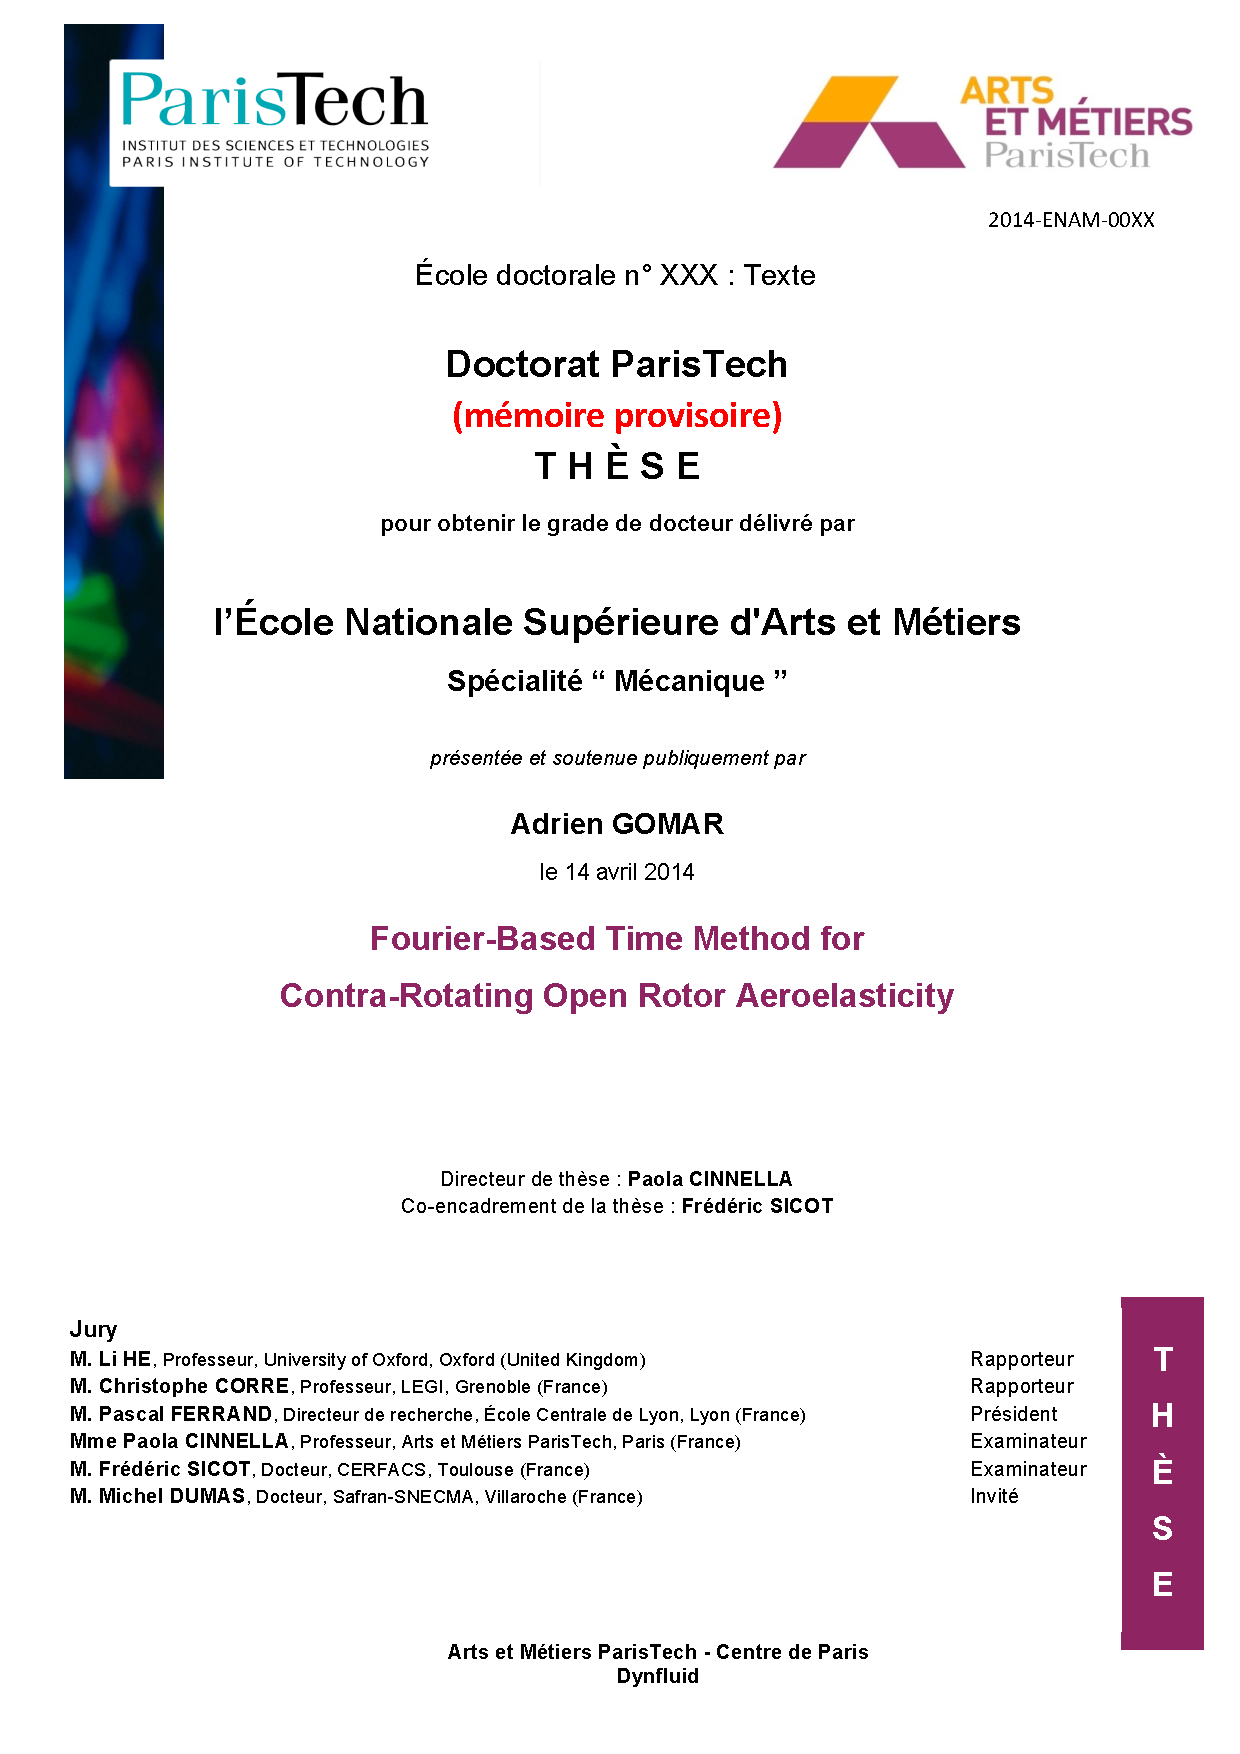
\includepdf{PARTS/OTHER/couv-ProvisoireTheseAMP.pdf} 

\cleardoublepage
%!TEX root = ../../adrien_gomar_phd.tex

\setlength\epigraphrule{1.5pt}
\setlength{\epigraphwidth}{0.55\textwidth}
\thispagestyle{empty}
\vspace*{100pt}

\epigraph{\textit{\Large It's better to regret something you did than something you didn't do}}%
{Deep Kick -- One Hot Minute\\ \textsc{Red Hot Chili Peppers}}


% %!TEX root = ../../adrien_gomar_phd.tex

\chapter*{Acknowledgments}
\thispagestyle{empty}

What a pleasure to finally write those lines !! This means that
the end is close ;)
I will try to make this quick, even though everyone knows that this
will be the most read part in this manuscript, starting by you ;)
I am not fooling myself.

First, I want to thank the members of the jury. I have been
delighted by the meticulous review made by Professor Li He and Professor 
Christophe Corre on this manuscript. Your remarks, observations
and questions
have participated to make this manuscript more complete and accurate, and
for that I thank you.
Then I want to thank the other members of the Jury: Pascal Ferrand, 
Jean-Camille Chassaing and Clément Dejeu for being here on D-Day,
for the chats that we had
and for the feedback that you gave me. This PhD defense day will remain as one of the
best days of my life, yet stressful.
As for the PhD defense, I will now switch in French as it will
be easier for me to make proper acknowledgments.

Je te tiens à remercier chaleureusement Paola Cinnella, ma
directrice de thèse. Pendant ces trois années, tu as été un pilier
de cette thèse et ce malgré la distance. 
Je te remercie d'avoir pris le temps à chaque fois
de m'aiguiller dans les choix "stratégiques", de remettre en cause
certaines de mes certitudes, et surtout pour ton regard neuf sur les méthodes
spectrales. J'ai beaucoup apprécié travailler avec toi.
Je tiens aussi à remercier Fredéric Sicot, mon encadrant au CERFACS.
Merci pour le temps que tu as pris pour m'expliquer les fondements de 
la TSM (même s'il faudrait mieux que je l'appelle HB, right ;)
et aussi pour le temps que tu as passé avec moi sur elsA. 
Merci surtout de m'avoir laissé la liberté et le temps
d'explorer des pistes parfois farfelues, j'ai beaucoup appris 
des réussites, mais surtout des échecs. Enfin, merci à Jean-françois Boussuge
de m'avoir accepté dans l'équipe AAM.
Je me rappellerais du son
de tes pas se dirigeant vers mon bureau ;) avec
en prime une remise en cause "douce" de certains de mes choix.
Cela m'a permis de m'affirmer là où j'étais encore trop
peu sur de moi, donc merci ! A contrario, je me rappellerais aussi 
de cette boite de chocolat pour nous remercier pour Antares :P
Un peu de douceur dans ce monde de brute right ?

Je souhaiterais remercier chaleureusement
l'ensemble de l'équipe AAM. Cela va être long et je vais
essayer d'oublier personne: je me lance. 
Merci Nico d'avoir cru en moi sur un simple coup
de téléphone. Merci pour ta bonne humeur quelque soit les
circonstances et ta gentillesse lorsque je suis venu te solliciter
pour la relecture de mon mémoire. Au passage désolé de ne pas
t'avoir payé cette dernière bière. Je n'ai pas trouvé le temps de t'inviter
en tête à tête au pub ... Merci Guillaume pour m'avoir encadré
sur mon stage. J'aurais aimé que cette thèse se passe avec toi comme
encadrant car j'ai toujours aimé la pédagogie que
tu prends pour expliquer les choses. 
Néanmoins, merci d'être resté dans les parages et d'avoir
continué à bosser avec nous !
Merci Marco, Lokmann
et JC, mes acolytes de stage. Je me suis marré pendant 6 mois.
Je me rappellerais de cette clim improvisée et des craquages de Marco !!
JC, encore toi, bah oui car comme moi tu es resté en thèse ;)
Merci pour ta gentillesse à toute épreuve ! Merci Sophie de
la team acoustique. Je suis désolé, tu as été ma target préférée
de fin de thèse, mais bon je t'ai toujours charriée en toute amitié,
j'espère que tu ne m'en voudras pas ;) 
Merci à l'autre belge de notre équipe, hein Nadège!! 
Sacré maman, un vrai petit caractère comme il faut !! Merci Benjamin
pour tous nos échanges sur le CROR. Avant nos discussions, je n'y
comprenais rien ;) merci pour ta vision physique et tous les échanges
que l'on a pu avoir sur nos thèses respectives. Cela fait du bien
d'échanger right ? Et merci d'avoir créé le terme "script jetable",
cela restera dans mon vocable. Merci à Thomas. J'ai adoré bosser avec
toi !! Je pense que dans un autre contexte, j'aurais cherché à
monter une boite avec toi !! Merci aussi pour cette visite personnalisée
de Bordeaux avec son fameux plan d'eau ... No comment. Pour moi tu es
devenu un véritable ami. Merci Gaëlle
pour ta fraicheur et pour m'avoir pris un nombre de jetons incalculables.
Je ne doute pas que ta thèse va bien se passer.
Merci à Remy, le plus AAM des combus, pour ton opiniâtreté sur Paraview.
Je te l'accorde, Paraview sait faire des smileys, 
mais non je ne l'utiliserais pas ;)
Merci à Bill bocquet et Flore. L'ex bureau improbable mais pourtant
bien là. Vous m'avez bien fait marrer. Je n'oublie pas Majd, Carlos et Julien.
La relève. Bon courage pour la thèse et faites ça dans la bonne humeur, vous
verrez la fin est vraiment agréable !
Merci à Marc, marcounet pour les intimes, merci d'avoir accepté de me prêter à taux
zéro des
jetons lorsque je n'en avais plus. Quand tu veux en Angleterre pour un
potage tomate !! Merci à Vieux gui pour les midi baby foot. J'aurais aimé
te battre un peu plus, car ton jeux m'a toujours déconcerté !! 
Merci à Guillaume pour ces bons chocolats et NON, Antares n'est pas buggé !!
C'est juste le mec qui est entre la chaise et le clavier ... 
énigme quand tu nous tiens ;) 
Merci Pierre d'avoir repris mon appart ! J'espère que tu t'y plairas
(même si je n'en doute pas un instants !).
Last but not least, merci à François pour ces
trois années de travail / déconnade / craquage le vendredi soir / 
petits gateaux / python / et de Pink Floyd qui claque. J'ai vraiment
eu le bureau qu'il fallait pour bosser et lâcher la pression de temps
en temps (souvent ?). Et non, je ne te remercierais pas
pour tes questions sur Git. J'ai jamais compris comment 
un mec aussi brillant pouvait avoir du mal
avec un soft aussi banal. Faut croire qu'il n'y a pas de règles ;)
Je n'oublie pas les CERFACSiens qui ont quitté le navire entre temps:
Antoine, Grace et Lulu.
Je n'oublie pas non plus l'équipe CSG. Merci Gérard,
tu as supporté mes coups de fil répétés, Fabrice pour ton
support sur les macs, Isabelle pour les problèmes de
compilation. C'est votre équipe qui fait la force du CERFACS.
Enfin, merci à L'administration du CERFACS, Michèle pour tes
conseils éclairés sur les aspects légaux, Marie pour
ton aide au jour le jour et pour faire le relais des 
congés !! Nicole, notamment pour ta relecture et les
corrections que tu as apportées sur notre premier
article. Lydia et Brigitte, pour votre accueil
et votre aide au quotidien.
Enfin merci à Chantal pour ta bonne humeur, pour 
cette bonne galette et pour t'être occupé de
Nahel pendant la soutenance, même si je ne pense
pas que c'était un calvaire pour toi !

Je souhaiterais aussi remercier Nicolas Binder et
Xavier Carbonneau. 
Merci de m'avoir initié au monde des turbomachines ;) Pour moi,
le débit c'est dieux et personne ne croit en l'expérience
sauf celui qu'il l'a faite et tout le monde croit en la
simulation sauf celui qu'il l'a fait. 
C'est ça que je devais retenir, right ?
Merci d'avoir pris le temps de 
discuter avec moi de mes travaux de thèse même si
vous n'étiez pas directement impliqués.
Merci à Yann Colin pour les échanges que l'on a pu avoir
sur les CRORs, mais surtout sur mon avenir. Aujourd'hui,
je suis convaincu que j'ai fait le bon choix et je te remercie
de m'avoir aiguillé !
Merci à Thieu pour m'avoir mis sur la voie de la CFD ;)
Aujourd'hui, on peut le dire, je ne porte plus de moufles, enfin
j'espère ...

\newpage

\`A la fin, il reste les amis et la famille ...
Merci à mon poto Remy pour les afterworks nécessaires
à la réussite de cette thèse. Merci aussi pour avoir été
là quand ça n'allait vraiment pas et aussi quand ça
allait pour fêter ça. Merci d'être venu à la soutenance.
Merci aussi à May d'avoir fait le déplacement, même
si le sujet, well, n'était pas trop ta tasse de thé.
Merci à mes frères Aurélien et Victor, à Salomé et à mes
Parents (I mean lolosse of course, l'autre ne t'arrive pas
à la cheville) pour votre soutien au cours de ces trois années.
On se rend pas compte à quel point votre présence m'a permis de
me dépasser. Merci aussi à JC, Cécile et la famille Hugon, passez 
nous voir en Angleterre quand vous voulez. Merci enfin à Géraldine, celle qui 
m'accompagne depuis tant d'années. Merci pour les coups
de pieds que tu m'as mis quand il fallait et pour ton
amour au quotidien. Cette thèse a été réussie grace à ton aide,
ton soutien et ta compréhension lors de ces longues nuits 
de travail et ces moments de doutes. Merci m’avoir soutenu. Je t'aime.
Merci enfin au petit nouveau de ma famille, mon fils Nahel.
Même si tu m'as donné du fil à retordre avant ma soutenance,
cela se voit déjà que tu es un gentil. Je t'aime.

\flushright{\emph{\`A Paris, le 6 mai 2014}}


\tableofcontents

% \cleardoublepage
% \addcontentsline{toc}{chapter}{\listfigurename}
% \listoffigures

% \cleardoublepage
% \addcontentsline{toc}{chapter}{\listtablename}
% \listoftables

% %!TEX root = ../../adrien_gomar_phd.tex

\chapter{Nomenclature}




%!TEX root = ../../adrien_gomar_phd.tex

\chapter{Introduction}

Global warming may be one of the biggest challenge that human kind
will have to face in the forthcoming decades if not years.
According to the last scientific
report of the Intergovernmental Panel on Climate Change 
(IPCC)~\cite{IPCC2013}
"The largest contribution to total radiative 
forcing\footnote{namely global warming} 
is caused by the increase in the atmospheric 
concentration of $CO_2$ since 1750".

A part of these $CO_2$ emissions and in general pollutants stems from the
transport industry and in particular the
aeronautical industry. 
Hopefully for the earth,
the rarefaction of crude oil accelerates the decision making.
In particular, in the seventies, the two oil crisis showed the aeronautical 
industries its dependence toward energy resources. 
To face this issue, the U.S. Senate directed NASA in 1975
to look for every potential fuel-saving concept for aircraft
engines. The Advanced Turboprop
project was born~\cite{Hager1988} and led to the
concept of contra-rotating open rotor. This new
engine concept showed large fuel savings
along with higher noise emissions due to the absence of
a duct. Combined with the decrease of the price of the
barrel in the late eighties, the contra-rotating open rotor 
never reached the commercial aviation.

Today, the cost of the barrel is almost at its maximum as shown
in Fig.~\ref{fig:crude_oil_price}.
\begin{figure}[htp]
  \centering
  \includegraphics*[width=0.40\textwidth]{crude_oil_price.pdf}
  \caption{Evolution of the cost of a barel from $1861$ to $2012$, from BP~\cite{bpreview2013}.}
  \label{fig:crude_oil_price}
\end{figure}
In parallel, Airbus forecasts a doubled number of passengers in
$2031$~\cite{AirbusForecast2013}. For that reason, the European commission has set, through the
Advisory Council for Aeronautics Research in Europe (ACARE),
demanding objectives to reduce these emissions for 2050:
the noise, $CO_2$ and $NO_x$ emissions should be reduced by 
$65\%$, $75\%$ and $80\%$, respectively
(Figure~\ref{fig:flightpath_2050}).
\begin{figure}[htp]
  \centering
  \includegraphics*[width=0.40\textwidth]{flightpath_2050.pdf}
  \caption{European Commission goals for the aeronautical industry.}
  \label{fig:flightpath_2050}
\end{figure}
Therefore, to allow a sustainable air transportation, new
concepts are needed for both the engines and the 
aircraft in general.
Several have emerged, among which lightweight construction
with advanced composite structure, airport collaborative decision
making with continuous climb departure and less waiting in taxi,
aerodynamically optimized wing geometries as laminar wings for instance
and finally fuel efficient engines to name but a few.
For the latter, two main types of engine are currently studied: the
High ByPass Ratio (HBPR) engine that is based on a
large diameter engine improving thus the
propulsive efficiency, and the Contra-Rotating Open Rotor (CROR)
engine that relies on two rows of contra-rotating propellers
that proves its viability during experiments within the framework of
the previously mentioned Advanced Turboprop project of NASA~\cite{Hager1988}.
\newline 

The industrial design of turbomachinery, and by extension contra-rotating
open rotors, is usually based on steady flow analysis, 
for which the reference simulation tool are the three-dimensio\-nal Reynolds-Averaged 
Navier--Stokes (RANS) steady computations. However, this approach finds its limits 
when unsteady phenomena become dominant. This is the case of 
contra-rotating open rotors where the interaction between the
two rotors is of prior importance. 
In such a
context, engineers need now tools to account for these effects as
early as possible in the design cycle. With the growth of
computational power, unsteady computations are entering industrial
practice, but the associated restitution time remains an obstacle for
daily basis applications.  For this reason, efficient
unsteady approaches are receiving a lot of attention. 

At CERFACS, several unsteady approaches have been investigated 
to reduce the computational time associated with the unsteady simulation of 
CROR configurations. 
These are seldom carried on the whole
circumference of the annulus due to the high computational
cost. A first approach is therefore to assume cyclic periodicity,
which allows to solve for only one blade passage and thus drastically
reduce the computational domain. 
In the turbomachinery community, the phase-lag approach has shown to be
a very efficient method to reduce the computational domain while
maintaining a good capture of the unsteady flow physics. 
In this way, \citet{Burnazzi2010} evaluated the phase-lag approach, largely
used in the turbomachinery community, by applying it
to a 3D contra-rotating open rotor configuration. He showed
that the interactions between the two rotors can be retrieve, allowing
thus a large computational time reduction.
A second approach 
is to work on the time-integration algorithm to reduce
the computational cost compared to standard time-marching techniques. To achieve
this, Fourier-based methods for periodic flows have undergone major
developments in the last decade (see \citet{He2010} for a recent
review).  The basic idea is to decompose
time-dependent flow variables into Fourier series, which are then
injected into the equations of the problem. The time-domain problem is
thus made equivalent to a frequency-domain problem, where the complex
Fourier coefficients are the new unknowns. At this point, two
strategies coexist to obtain the solution. The first one is to solve
directly the Fourier coefficients, using a dedicated
frequency-domain solver, as proposed by \citet{He1998}. The second strategy is to cast the
problem back to the time domain using the inverse Fourier transform, as
proposed by \citet{Hall2002} with the Harmonic
Balance (HB) method. The unsteady time-marching problem is thus
transformed into a set of steady equations coupled by a source term
that is a high-order spectral evaluation of the time-derivative of the
initial equations. The main advantage of solving in the time domain is
that it can be implemented in an existing classical RANS solver,
taking advantage of all classical convergence-accelerating techniques
for steady state problems.
\citet{ThesisSicot} implemented
the HB method into the \textit{elsA}~\cite{Cambier2013} CFD code
that is used at CERFACS. Applied to turbomachinery
configurations, this method showed a computational gain
of one to two orders of magnitude 
compared to classical time-marching approaches.
Applied to CROR configurations, \citet{Yabili2010}
showed that the computational time reduction
was not conclusive. In fact, a large number of 
harmonics compared to turbomachinery configurations
was needed to properly capture the unsteadinesses, lowering
the computational gain.
Therefore, \citet{ThesisFrancois} deeply
investigated the different unsteady approaches available 
for turbomachinery computations, among which the HB approach, 
and evaluated it for CROR simulations. 
He confirmed that
the harmonic balance method can retrieve unsteady
flow features for a reduced cost at a gain that
is relatively smaller compared to what was
obtained on former turbomachinery applications.
In parallel, \citet{ThesisGuedeney} extended the harmonic
balance approach to a multi-frequential framework. 
This method allows then to compute unsteadinesses whose frequencies
are not harmonically related, which opens new perspectives.
\newline

Several challenges, such as aerodynamic,
aeroacoustic and aeroelasticity are still open 
for contra-rotating open rotor
to become a viable engine for the next generation aircraft.
In this PhD thesis, we propose to assess the aeroelasticity of 
contra-rotating open rotor by using the multi-frequential
harmonic balance approach developed and implemented 
by \citet{ThesisGuedeney}.
Actually, the main unsteadinesses of the flow field
are known to be correlated with the so-called
blade passing frequency. This frequency depends on the
rotation speed of the current rotor and the opposite rotor
number of blades. In contrast to that, the 
frequency that drives the aeroelasticity of CROR
blades depends on their structural properties.
As such, the frequencies of both the aerodynamic
field and the aeroelasticity are not harmonically
related, which justifies the use of the multi-frequential
formulation of the harmonic balance approach.


The aim of this PhD thesis is to assess the
multi-frequential harmonic balance
to estimate the flutter properties of contra-rotating open rotor
configurations. In this way, the memoir is divided in three parts:
\begin{itemize}
	\item \hyperref[part1]{\emph{Part I}} presents general information on 
	contra-rotating open rotors (\hyperref[cha:cror]{\emph{Chapter~1}}),
	the basic equations that govern the aeroelasticity of
	turbomachinery and CROR are then presented and the approach retained 
	to simulate it is detailed (\hyperref[cha:ael]{\emph{Chapter~2}}).
	Finally the mathematical mechanisms that allow the derivation
	of Fourier-based time methods and their underlying properties
	(\hyperref[cha:spectral_methods]{\emph{Chapter~3}}) are presented and the 
	multi-frequential harmonic balance approach is chosen.
	\item \hyperref[part2]{\emph{Part II}} 
	presents the advantages and limitations
	of Fourier-based time methods. The chosen approach, namely
	the harmonic balance, is validated for linear and non-linear
	equations in \hyperref[cha:validation_hb]{\emph{Chapter~4}}. Both the
	mono-frequential and the multi-frequential formulations
	are shown to give spectral accuracy, which is a convergence
	property specific to Fourier-based time methods.
	It is emphasized
	that a large CPU gain can be expected in the
	case of contra-rotating open rotor aeroelasticity. 
	Sadly, when using the multi-frequential harmonic
	balance, mathematical properties can lead to divergence
	of the computation through a high condition number
	(\hyperref[cha:limitations_condition_number]{\emph{Chapter~5}}). This is 
	first highlighted on two toy problems and then cured using
	an original optimization algorithm.
	Finally, the convergence of the harmonic balance 
	that was shown to be case dependent is
	assessed (\hyperref[cha:limitations_convergence]{\emph{Chapter~6}}). 
	It is demonstrated that the difference in computational
	gain is linked to the thickness of the wakes observed behind
	turbomachinery blades, which extends to CROR blades. Based on this observation,
	a prediction tool is developed to estimate the
	number of harmonics needed to compute a given turbomachinery (and CROR)
	configuration using a mixing plane computation 
	The relative CPU gain to be expected can thus be estimated
	and help the decision making in choosing an unsteady approach
	over another one.
	\item based on the work done in the second part,
	the proposed approach retained in this thesis, 
	namely the multi-frequential harmonic balance method along with a weak 
	aeroelastic coupling approach, is applied on different configurations
	in \hyperref[part3]{\emph{Part III}}. Firstly, it is validated 
	on a reference configuration against experimental 
	results and other numerical approaches found in the literature
	(\hyperref[cha:stcf11]{\emph{Chapter~7}}). This give us confidence
	to apply the approach on an industrial isolated contra-rotating
	open rotor application at low-speed (\hyperref[cha:dream_ls_isolated]{\emph{Chapter~8}})
	and high-speed (\hyperref[cha:dream_hs_isolated]{\emph{Chapter~9}})
	flight conditions. The aeroelastic results are discussed based
	on the computed unsteady flow field.
\end{itemize}


\mainmatter

\part{General information}
\label{part1}
%!TEX root = ../../../adrien_gomar_phd.tex
\chapter{Contra-rotating open rotors}
\label{cha:cror}

\chabstract{In this chapter, we first recall the thrust
and propulsive efficiency equations. Using them,
the propeller engines are shown to be good candidates
for efficient alternative engines, mainly due to a high bypass ratio.
Geometry, general principles, similarity coefficients
and main physical phenomena of such engines are 
described. In addition to that, it is shown that even if efficient,
propeller engines suffer from a residual swirl motion.
To tackle this problem, the contra-rotating open rotor
technology is presented along with its main source of unsteadiness.
The challenges associated to this engine are finally detailed
and we show that aeroelasticity needs to be accounted for.}


\newpage

\section{Generalities of propulsion}
\label{sec:cror_intro}
%!TEX root = ../../../adrien_gomar_phd.tex

For an aircraft in steady flight conditions, 
lift balances weight and 
thrust balances drag. This explains why engineers try
indefinitely to reduce weight while increasing
thrust. A trade-off between those two is to work
on the propulsive efficiency of the engine. In this
section, general information on propulsion
that leads to the concepts of propeller and
contra-rotating open rotor are given.

\subsection{Thrust equation}
\label{sub:cror_thrust}
Consider the conservative equation of momentum
\begin{equation}
	\frac{\partial \rho \vec{V}}{\partial t} 
	+ \nabla \cdot (\rho \vec{V} \otimes \vec{V} + p \mathbb{I} - \vec{\vec{\Sigma}}_v) = 0,
\end{equation}
where $\rho$ is the density, $\vec{V}$ the velocity vector, $p$ the pressure and
$\vec{\vec{\Sigma}}_v$ the viscous stress terms.
Consider two closed domains $\Sigma$ and $\Sigma^\prime$ as
shown in Figure~\ref{fig:cror_control_volume}.
\begin{figure}[htp]
  \centering
  \includegraphics*[width=0.30\textwidth]{control_volume.pdf}
  \caption{Domains used for the application of the momentum equation.}
  \label{fig:cror_control_volume}
\end{figure}
The domain $\Sigma^\prime$ represents a fluid domain outside from the
engine encompassed by the solid domain $\Sigma$.
Taking a steady state hypothesis, one can write
\begin{equation}
	\oint_{\Sigma} \left(\rho \vec{V} \otimes \vec{V} + 
	                       p \mathbb{I} - 
	                       \vec{\vec{\Sigma}}_v \right) \cdot \vec{n} \diff S
    =
   	\oint_{\Sigma^\prime} \left(\rho \vec{V} \otimes \vec{V} + 
	                       p \mathbb{I} - 
	                       \vec{\vec{\Sigma}}_v \right) \cdot \vec{n} \diff S,
\end{equation} 
where $\vec{n}$ is the normal vector.
As $\Sigma^\prime$ is an arbitrary domain, we can take it sufficiently
away from the engine so that $\vec{\vec{\Sigma}}_v$ becomes zero (\emph{i.e.}
viscosity stress terms are null).
Moreover, 
\begin{equation}
	\oint_{\Sigma} \left(\rho \vec{V} \otimes \vec{V} \right) \cdot \vec{n} \diff S = 0,
\end{equation}
since the surface is solid ($\vec{V} = \vec{0}$ on wall). 
If $\vec{F}$ denotes the resultant forces acting on $\Sigma$
\begin{equation}
	\vec{F} = \oint_{\Sigma} \left(p \mathbb{I} - 
	\vec{\vec{\Sigma}}_v \right) \cdot \vec{n} \diff S,
\end{equation}
then
\begin{equation}
	\vec{F} = \oint_{\Sigma^\prime} \left(\rho \vec{V} \otimes \vec{V} +
	p \mathbb{I} \right) \cdot \vec{n} \diff S.
\end{equation}
Assuming that $\Sigma^\prime$ is a stream tube, and projecting the equation
onto the $x$-axis gives the formula for the thrust $F_x$
\begin{equation}
	F_x = \dot{m} V_{out} + p_{out} S_{out}
	- \dot{m} V_{in} - p_{in} S_{in},
\end{equation}
using the notation of Figure~\ref{fig:cror_control_volume}.

Far downstream of the engine $S_{in} = S_{out}$ and
considering that we have an adapted nozzle ($p_{in} = p_{out}$),
the thrust $F_x$ can be written as
\begin{equation}
	\fbox{$
	F_x = \dot{m} (V_{out} - V_{in}) = \dot{m} \Delta V_x
	$}
	\label{eq:cror_thrust}
\end{equation}
where $\dot{m}$ is the mass-flow rate going through the
propeller and $\Delta V_x$ is
the increment of axial velocity. From this simple equation,
one can see that to increase the thrust $F_x$, there are two parameters:
the mass-flow and the axial velocity increment.

\subsection{Global propulsive efficiency}
\label{sub:cror_efficiency}

The global propulsive efficiency $\eta$ measures the 
success in converting a mechanical power into a
propulsive power. It results from the combination
of the kinetic efficiency $\eta_{K}$ and the propulsive efficiency
$\eta_{PR}$
\begin{equation}
	\eta = \eta_{K} \times \eta_{PR}.
\end{equation}
This is schematically represented in Figure~\ref{fig:cror_efficiency}.
\begin{figure}[htp]
  \centering
  \includegraphics*[width=0.40\textwidth]{efficiency.pdf}
  \caption{Efficiency relations from mechanical power to propulsive power.}
  \label{fig:cror_efficiency}
\end{figure}

\paragraph{Kinetic efficiency}
The kinetic efficiency measures the success in converting the mechanical
power $P_m$ into a kinetic power $P_k$
\begin{equation}
	\eta_K = \frac{P_k}{P_m}.
\end{equation}

The mechanical power delivered as input
can be computed through the first thermodynamic principle. In fact, in absence
of heat exchange, the mechanical power $P_m$ can be estimated as
\begin{equation}
	P_m = \dot{m} (h_{i_{out}} - h_{i_{in}}),
\end{equation}
where $h_i$ is the total enthalpy and subscript $in$ and $out$ are
the input and output, respectively, of the propulsion system as represented
in Figure~\ref{fig:cror_control_volume}.
The kinetic power $P_k$ is given by
\begin{equation}
	P_k = \dot{m} \left(\frac{1}{2} V^2_{out} -
	\frac{1}{2} V^2_{in} \right).
\end{equation}
This leads to a kinetic efficiency that can be expressed as
\begin{equation}
	\eta_{K} = \frac{V^2_{out} - V^2_{in}}{2 (h_{i_{out}} - h_{i_{in}})}
\end{equation}

\paragraph{Propulsive efficiency}
The propulsive efficiency $\eta_{PR}$ measures the success
in creating a propulsive power $P_{pr}$ from a
kinetic power $P_k$
\begin{equation}
	\eta_{PR} = \frac{P_{pr}}{P_k}.
\end{equation}
The propulsive power is computed using the thrust $F_x$
\begin{equation}
	P_{pr} = F_x \times V_{\infty},
\end{equation}
where $V_{\infty}$ is the free-stream velocity.
Finally, if the free-stream velocity is the inlet velocity $V_{in}$
and the inlet and outlet velocities are purely axial
\begin{equation}
	\fbox{$
	\eta_{PR} = \displaystyle \frac{1}{1 + \frac{V_{out} - V_{in}}{2 V_{in}}}
	$}
	\label{eq:cror_propulsive_efficiency}
\end{equation}
This formula means that the most efficient engine produces
a very small velocity increment.

\subsection{Toward propeller engines}
\label{sub:cror_toward_propeller}

One way to improve the environmental footprint of
airplanes engines is to increase the propulsive efficiency
by reducing the kinetic power needed to drive the engine.
Doing so while maintaining the thrust can be achieved through
a higher mass-flow rate. Two new concepts are thus derived from
this simple statement: the High ByPass-Ratio (HBPR) which
is basically a turbofan with a larger fan exhaust, and the
propeller whose mass-flow rate is not limited
by the architecture, as the blades are not within a nacelle.
In the following section, the propeller engine will be detailed
and the drawbacks of such an architecture will be highlighted to
motivate the use
of a second propeller row, yielding the contra-rotating open rotor
architecture.




\section{Propellers}
\label{sec:cror_propeller}
%!TEX root = ../../../adrien_gomar_phd.tex

\subsection{Geometry}
\label{sub:cror_propeller_geometry}

A propeller is composed of a hub and a rotating set of 
$B$ blades as schematically represented in
Fig.~\ref{fig:cror_propeller_geometry}. The hub
is the part on which the blades are mounted.
We set the diameter of these blades being $D$
and their rotation speed being $\Omega$. 
In front of the propeller, there is a spinner which is
a conic geometry element that helps
smoothing the inflow for the propeller blades.
The propeller can be seen as
a turbofan whose fan is not within a nacelle.
\begin{figure}[htb]
  \centering
  \includegraphics*[scale=0.30]{propeller_geometry.pdf}
  \caption{Geometry of a propeller.}
  \label{fig:cror_propeller_geometry}
\end{figure}
Its absence implies that theoretically, the mass-flow can be
infinite. To quantify this, it is common for engines to
consider the bypass ratio. It is defined as the ratio between the
cold air (the un-combustioned air)
divided by the hot air (the air that goes through the engine core).
To give an idea, one of the highest bypass ratio engine on today's aircraft is given
by the Pratt~\&~Whitney~PW1000G and is~12, while propellers are estimated
to have a bypass ratio of~50. 
This number is representative of the mass-flow rate generated by the engine.
However, we have seen that mass-flow is a parameter that can be used to increase
the thrust so as the velocity difference. Assuming that in a classical ducted turbofan, 
the bypass ratio is limited to~12, the only
way to increase the thrust is to increase the 
velocity which deteriorates the propulsive efficiency. In absence of a duct,
no limitation is set by the nacelle on the mass-flow rate.
This explains why this architecture has
regained interest. However, propellers
have been limited to low Mach number flight condition
due to the high relative velocity seen at the tip of the blades.

\subsection{Velocity triangle}
\label{sub:cror_propeller_velocity_triangle}
The velocity triangle applied to a propeller configuration
is shown in Fig.~\ref{fig:cror_velocity_triangle_propeller}.
The aim of a propeller is to create thrust through an increase
of the axial velocity noted $\Delta V_x$ in the diagram. To do
so, the relative flow field is straighten up. This gives both
an increase in axial velocity but also in tangential velocity.
In fact, the inflow that was purely axial has a tangential
component at the outlet. This is called the swirl and
is a lost energy as it cannot be used to produce thrust.
\begin{figure}[htbp]
  \centering
  \includegraphics*[scale=0.40]{velocity_triangle_propeller.pdf}
  \caption{Velocity triangle applied to a propeller.}
  \label{fig:cror_velocity_triangle_propeller}
\end{figure}
Moreover, the relative velocity $W$ should be kept subsonic
otherwise the propulsive efficiency is reduced. This limits
the free-stream velocity $V_0$ of the aircraft and the size of 
the propeller as $U = \Omega R$.

\subsection{Similarity coefficients}
\label{sub:similarity_coefficients}
To evaluate the performances of the propeller, four similarity
coefficients are commonly used:
the advance ratio $J$ that represents the operating point of the propeller,
the thrust $C_t$ and power $C_p$ coefficients that estimate its performance and finally
the efficiency $\eta$:
\begin{equation}
    J = \frac{V_0}{n D}, \quad
    C_T = \frac{F_x}{\rho n ^ 2  D ^ 4}, \quad
    C_P = \frac{M_x \Omega}{\rho n ^ 3 D ^ 5}, \quad
    \eta = J \frac{C_T}{C_P},
\end{equation}
where $V_0$ is the free-stream velocity 
as shown in Fig.~\ref{fig:cror_propeller_geometry},
$\rho$ the free-stream density,
$n$ the rotation frequency ($n = \Omega / 2 \pi$) and
$M_x$ the axial torque.
The efficiency defined here is the global propulsive efficiency
as it gives the ratio of the propulsive power over the mechanical power.

An estimation of the variation of the advance ratio $J$ and the 
efficiency $\eta$ depending on the flight conditions can be given as follow
\begin{alignat}{4}
    \text{(cruise)} \quad  0.8 &< \eta &< 0.95, \quad 1 &< J < 3.5 \\
    \text{(take-off)} \quad  0.5 &< \eta &< 0.8, \quad J &< 1.
\end{alignat}

\subsection{Main physical phenomena}
\label{sub:cror_propeller_physics}

\begin{figure}[htb]
  \centering
  \subfigure[Wakes]{
      \label{fig:propeller_wakes}
      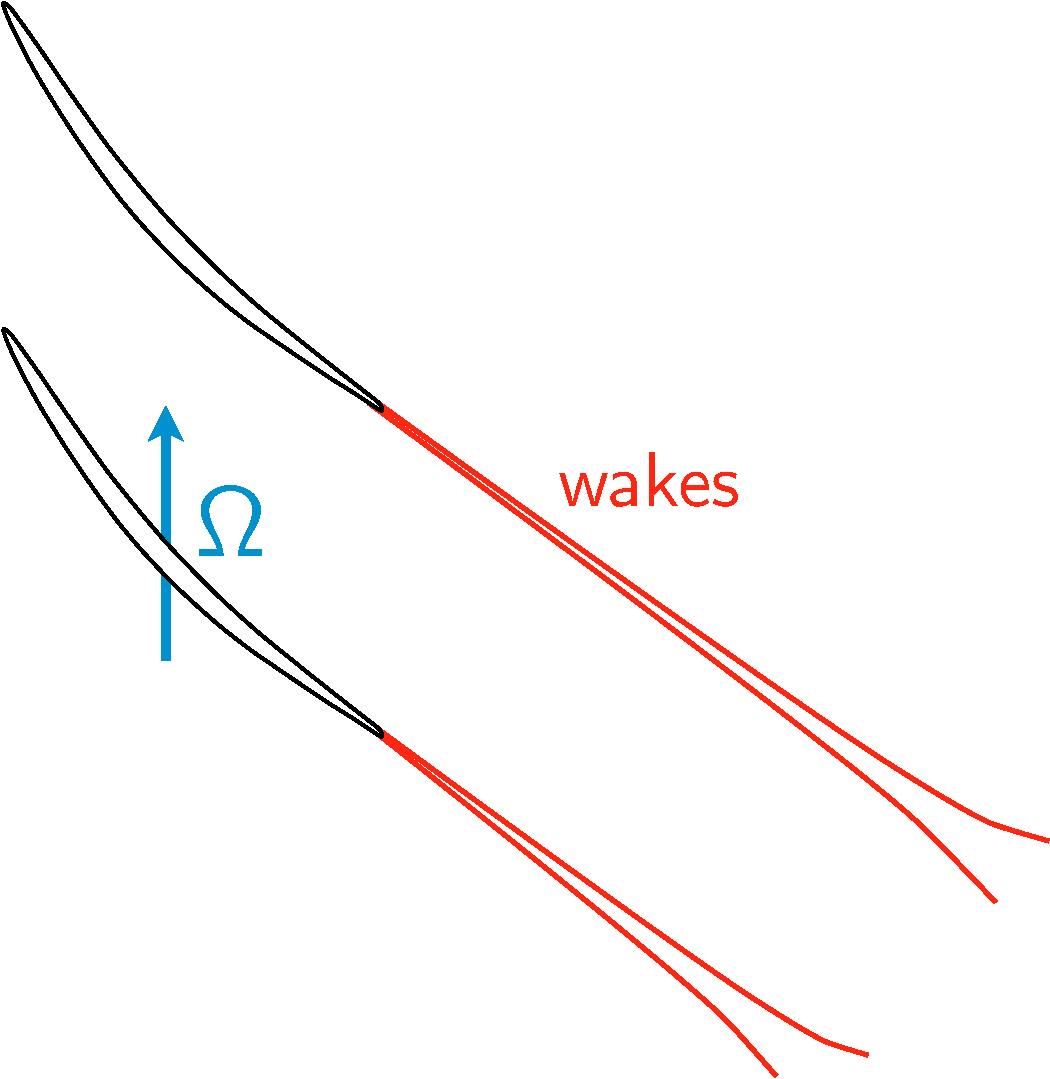
\includegraphics[scale=.2]{propeller_wakes.pdf}}
  \quad\subfigure[Tip vortices]{
      \label{fig:propeller_tip_vortices}
      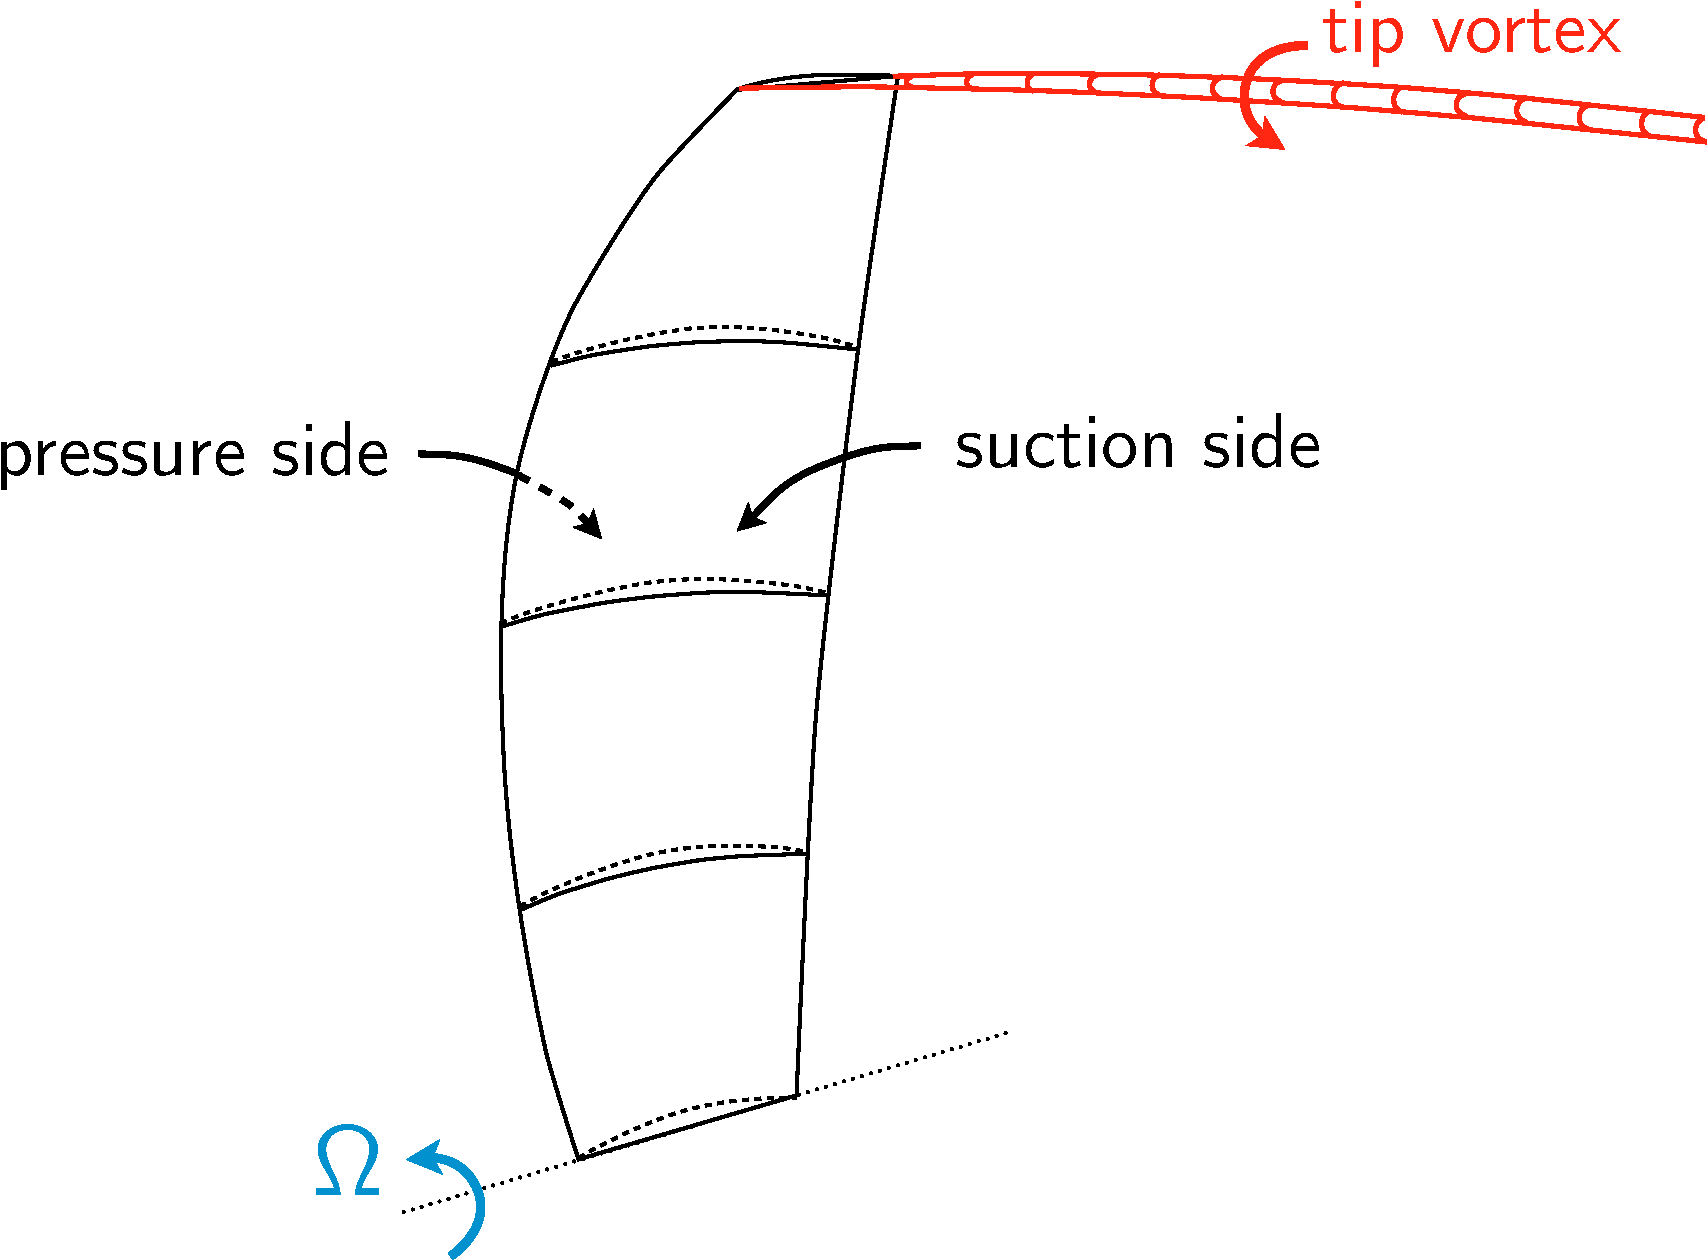
\includegraphics[scale=.2]{propeller_tip_vortices.pdf}}
  \quad\subfigure[Stream tube contraction]{
      \label{fig:propeller_stream_tube}
      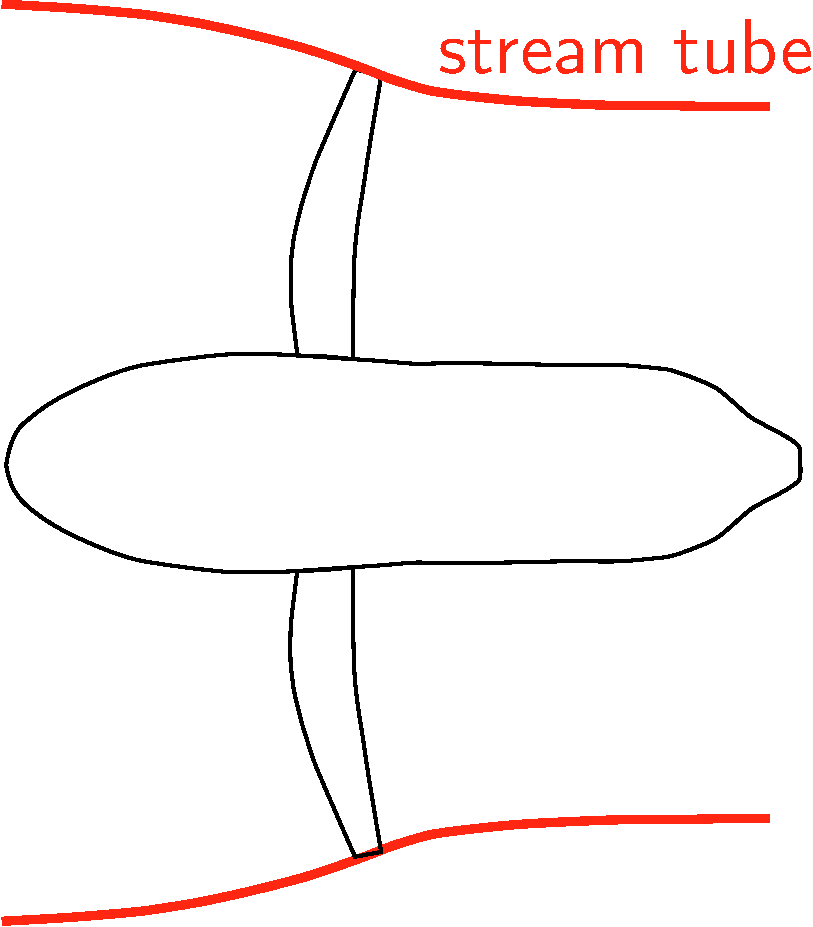
\includegraphics[scale=.2]{propeller_stream_tube.pdf}}
  \caption{Main physical phenomena seen in a propeller.}
  \label{fig:propeller_phys_phenomena}
\end{figure}
The main physical phenomena that can be seen in a propeller are schematically represented
in Fig.~\ref{fig:propeller_phys_phenomena}. Firstly, due to the presence of a boundary
layer on the pressure side and suction side of the blades, a wake is shed behind each blade, which
is represented by a momentum deficit. It is mostly a two-dimensional
phenomenon seen at each radii. Secondly, in the tip region of the blade, the pressure difference between 
the sides of the blade induces a vortex counter-rotating with respect to 
the rotation speed. Their convection is ensured by the local relative velocity giving them
an helical path propagating downstream.
To reduce this phenomenon, one way is to modify the geometry of the tip
of the blades but does not fully annihilate this phenomenon. 
Finally, the propeller generates thrust through an acceleration of the fluid. Thus, the stream
tube is contracted. All of these phenomena are stationary in their relative frame of reference.


\section{Contra-rotating open rotors}
\label{sec:cror_cror}
%!TEX root = ../../../adrien_gomar_phd.tex

As shown above in a single rotor propeller, the outlet velocity is not axial
yielding a residual tangential velocity $\Delta V_{\theta}$,
which forms the swirl. 
This is a lost energy that deteriorates the propulsive efficiency. 
To recover it, a second contra-rotating rotor can be used~\cite{Hager1988}.
We will see in this section through a simple velocity triangle exercise that
the swirl is annulated by the second rotor. This increases the propulsive
efficiency as shown by \citet{Hughes1989} and reported 
in Figure~\ref{fig:hughes_propulsive_efficiency}.
\begin{figure}[htp]
  \centering
  \includegraphics*[width=0.40\textwidth]{hughes_propulsive_efficiency}
  \caption{Benefit of using a contra-rotating open rotor, from \citet{Hughes1989}.}
  \label{fig:hughes_propulsive_efficiency}
\end{figure}

\subsection{Geometry}
\label{sub:cror_geometry}

Figure~\ref{fig:cror_geometry} depicts the main
geometrical parameters of a CROR.
It is composed of two rotors, the first one is called
the front rotor and the second one is called the rear or aft rotor.
Generally, they do not have the same diameter and rotation speed. 
Thus, subscript $f$ and $r$ denotes respectively,
the front and the rear parameters.
The difference of diameter is called the clipping or cropping
of the blades and is evaluated through the non-dimensional parameter
$\kappa$
\begin{equation}
    \kappa = \frac{D_f - D_r}{D_f}.
\end{equation}
By clipping the rear
rotor, tip vortices shed by the front rotor are not likely
to hit the rear rotor blades.
Finally, the spacing between the rotors
is evaluated as the difference between the axial minimum of the
rear blade minus the axial maximum of the front blade. The spacing
is one of the adjustment parameters used to minimize the unsteady
interaction between the rotors to reduce noise. In fact, 
heterogeneities are lessened along with the convection of
the flow field. These heterogeneities are responsible
for the unsteady interactions and, by extrapolating, for noise generation.
\begin{figure}[htp]
  \centering
  \includegraphics*[scale=0.3]{cror_geometry.pdf}
  \caption{Contra-rotating open rotor geometrical parameters.}
  \label{fig:cror_geometry}
\end{figure}

Two types of contra-rotating open rotors have emerged, the
puller CROR whose blades are near the front of the spinner as 
shown in Figure~\ref{fig:cror_configurations}. As the
name indicates, this configuration is mounted in front of the
wing. It is particularly interesting as the blades will see
a uniform flow. However, these all suffer from the same incidence as that
of the wing. This can give large in-plane forces 
(forces normal to the rotation axis~\cite{ThesisFrancois}) compared to pusher
configurations. In opposite, the deflection of the flow due to the wing provides
a smaller incidence.
Moreover, the distortion generated
by the CROR will disturb the flow around the wing. As one way to reduce
consumption of airplanes is to have laminar wings, this configuration
is less studied. The second configuration is the pusher
configuration. It is designed to be mounted on a pylon which will thus
interact with the CROR, but laminar wings might be considered with
this configuration. In this thesis, we will deal with a pusher configuration
in Chapters~\ref{cha:dream_ls_isolated} and
\ref{cha:dream_hs_isolated}.
\begin{figure}[htp]
  \centering
  \subfigure[puller]{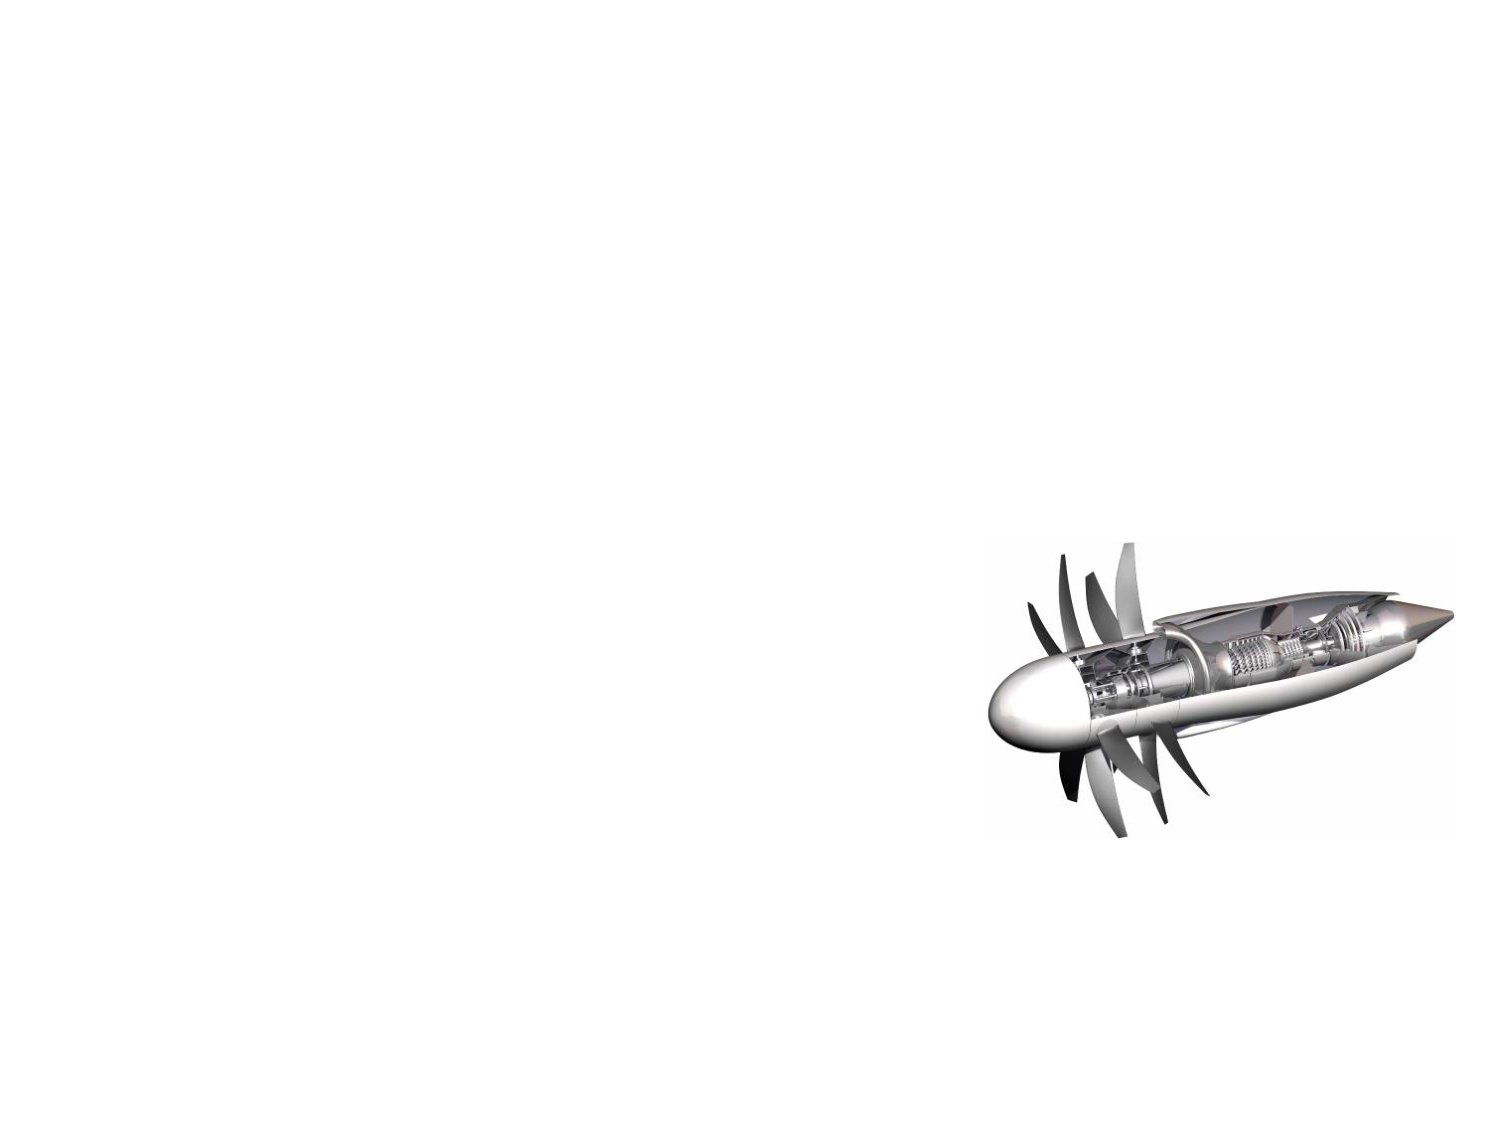
\includegraphics[width=.4\textwidth]{puller.pdf}}
  \subfigure[pusher]{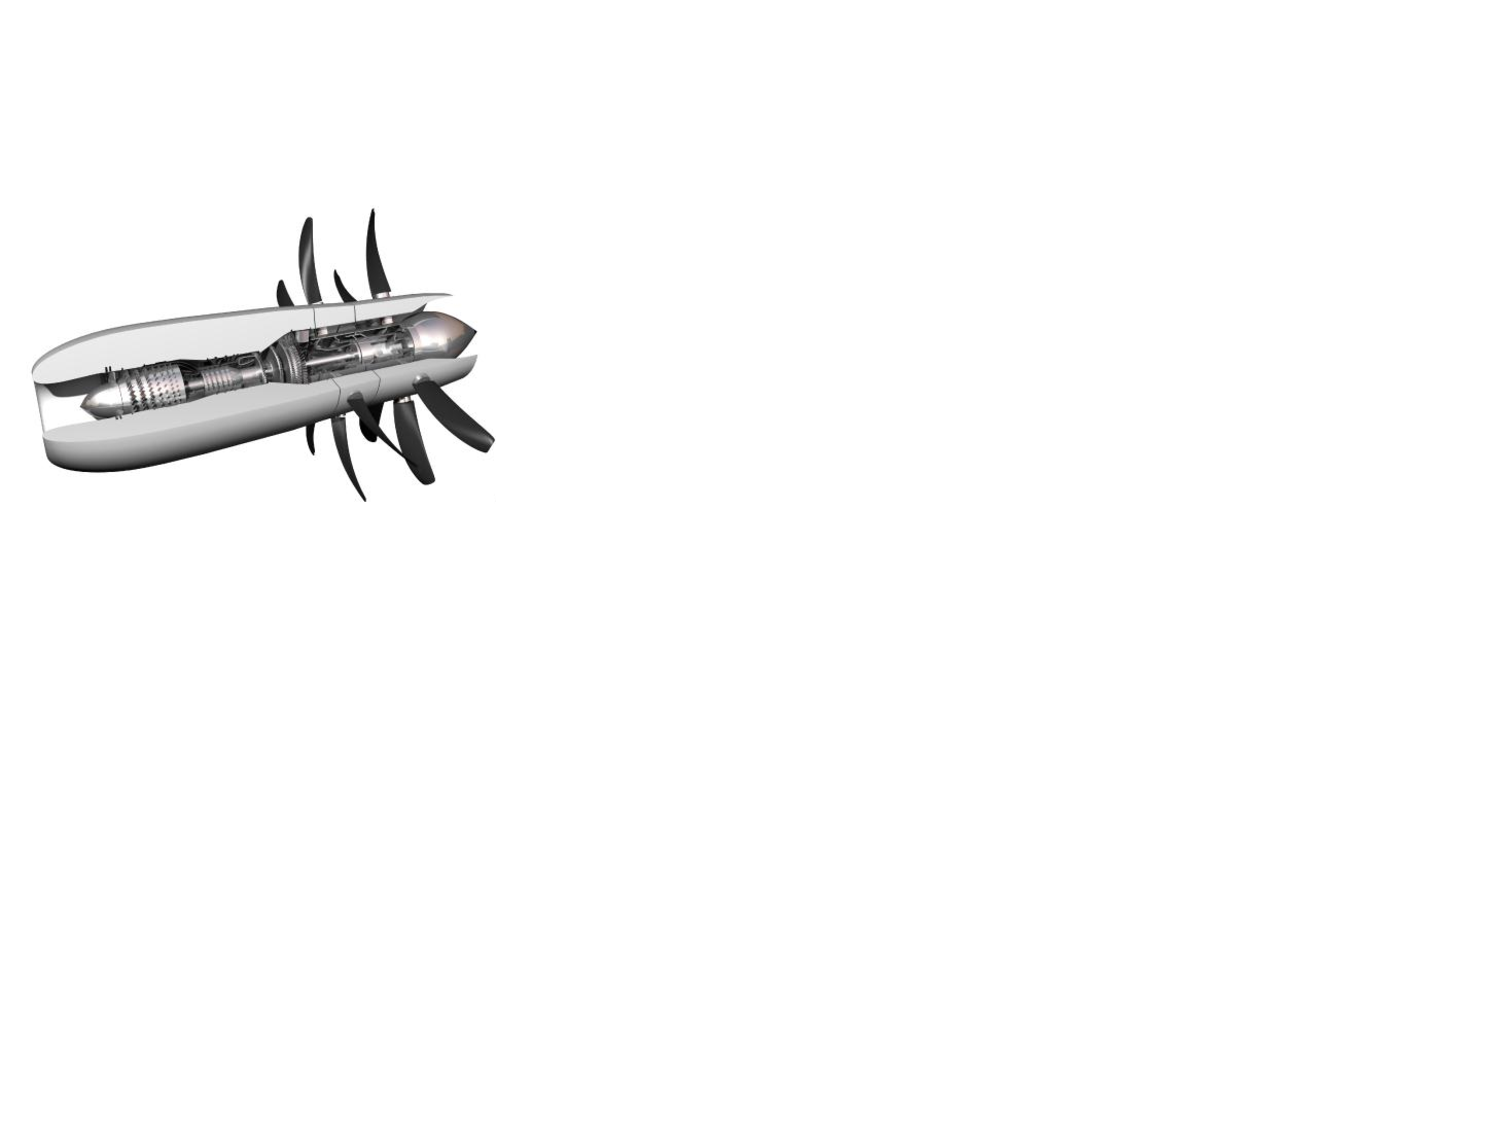
\includegraphics[width=.4\textwidth]{pusher.pdf}}
  \caption{Contra-rotating open rotor configurations, courtesy Rolls-Royce.}
  \label{fig:cror_configurations}
\end{figure}
% For pusher CROR, two types of architectures can be thought:
% one based on a gearbox and the second
% being build around a statorless low-pressure turbine. These
% two 
% \begin{figure}[htp]
%   \centering
%   \subfigure[geared design]{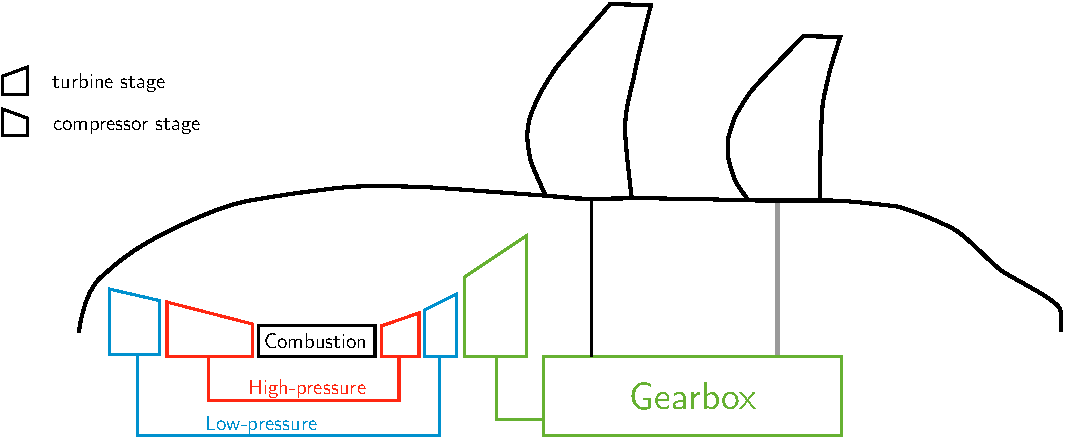
\includegraphics[width=.4\textwidth]{geared_cror.pdf}}
%   \subfigure[statorless low-pressure turbine design]{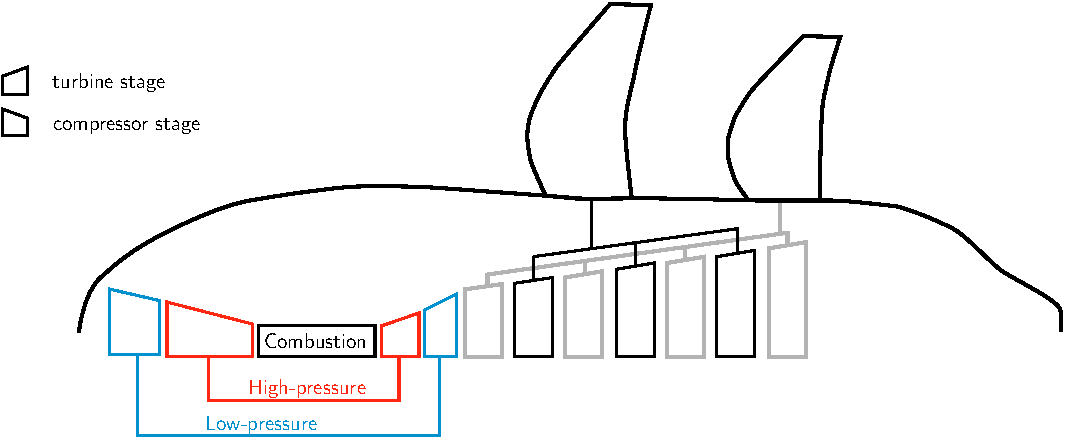
\includegraphics[width=.4\textwidth]{stator_less_cror.pdf}}
%   \caption{Contra-rotating open rotor pusher architectures.}
%   \label{fig:cror_architectures}
% \end{figure}

\subsection{Velocity triangle}
\label{sub:cror_velocity_triangle}
\begin{figure}[htp]
  \centering
  \includegraphics*[scale=0.5]{velocity_triangle_cror.pdf}
  \caption{Velocity triangle applied to a contra-rotating open rotor configuration.}
  \label{fig:velocity_triangle_cror}
\end{figure}
Figure~\ref{fig:velocity_triangle_cror} shows the application
of the velocity triangle to a CROR configuration. The swirl
energy that was lost by the propeller is now used to 
produce more thrust. Therefore, a CROR will finally have a better propulsive
efficiency than a propeller, which explains its study as
a greener engine. In the eighties, 
\citet{Strack1981} and \citet{Hager1988} showed that
using a contra-rotating open rotor technology over
a single propeller gave an increase of $6-8\%$
in propulsive efficiency, explaining its regain of interest.
Today, high-speed propellers blades might lead to higher increase
in efficiency
while keeping a flight Mach number close to $0.8$, enabling its use
for commercial aviation.

\subsection{Similarity coefficients}
\label{sub:cror_similarity_coeff}

In the case of a CROR configuration, the front and the rear rotors 
have to be considered.
Two main ways exist to evaluate the global value of the
similarity coefficients. The first one, chosen by
\citet{Bechet2011} among others, is to consider
that the non-dimensional parameter $D$, $n$ and $J$ are those
of the front rotor for both rotors
\begin{equation}
    J_f = J_r = \frac{V_0}{n_f D_f}, \quad
    C_T = \frac{F_{x_f} + F_{x_r}}{\rho_F n_f ^ 2  D_f ^ 4}, \quad
    C_P = \Omega_f \frac{M_{x_f} + M_{x_r}}{\rho_f n_f ^ 3 D_f ^ 5}, \quad
    \eta = J_f \frac{C_T}{C_P}.
\end{equation} 
The second one uses the non-dimensional parameter of the current rotor,
as done by \citet{Stuermer2008} and \citet{Zachariadis2011}.
The first approach is retained for the current work as it allows
to simplify the comparison of the similarity coefficient with equivalent propellers.


\section{Unsteadinesses}
\label{sec:cror_unsteady}
%!TEX root = ../../../adrien_gomar_phd.tex

\subsection{From steady to unsteady phenomena}
\label{sub:cror_from_steady_to_unsteady_phenomena}

The flow generated behind the front rotor
is steady in its frame of reference. Nevertheless,
due to the relative speed difference between the
front and the rear rotor, these steady flow distortions are
seen as unsteady features by the rear rotor. 
These unsteadiness are correlated to the Blade Passing Frequency (BPF):
\begin{equation}
	f = \frac{\Omega_{rel} B_{opp}}{2 \pi},
\end{equation}
where $\Omega_{rel}$ is the relative speed difference between
the current and the opposite row
and $B_{opp}$ the number of blades in the opposite row.

\subsection{Main unsteadinesses}
\label{sub:cror_main_unsteadinesses}

In sec.~\ref{sub:cror_propeller_physics}, the main physical phenomena
that appears in a propeller have been introduced. As seen above, due to
the relative speed difference between the two rotors, these phenomena
that were steady in their frame of reference are now seen as unsteady features
by the rear rotor. As such, to numerically simulate them, unsteady computations
will be needed. In this aim, the following section will be devoted to the classification
of unsteady phenomena that appears in CROR in 
order to choose an efficient strategy to simulate them.

\paragraph{Tip vortices}

As shown previously in Fig.~\ref{fig:propeller_tip_vortices}, tip vortices are formed
at blade tips due to the pressure difference between each side of the blades.
If nothing particular is done, this low momentum perturbation can
hit the rear rotor and induce large unsteady fluctuations. To avoid this,
the rear rotor blades are clipped as mentioned earlier. 
This unsteadiness is correlated with the BPF.

\paragraph{Wakes and potential effects}

Compared to an isolated rotor, as for the case of a propeller,
the presence of the rear rotor gives rise to an unsteady
interaction by means of potential effects. In addition, wakes generated
behind the front rotor interact with the rear rotor.
This is schematically represented in Fig.~\ref{fig:cror_wakes_potential}.
\begin{figure}[htp]
  \centering
  \includegraphics*[width=0.30\textwidth]{cror_wakes_potential.pdf}
  \caption{Wakes and potential effects in a 
  contra-rotating open rotor configuration.}
  \label{fig:cror_wakes_potential}
\end{figure}
These two phenomena are correlated with the blade passing frequency.
In addition to this, vortex shedding phenomena may occur behind the blades, 
the frequency being not known a priori.
This phenomenon is more likely to appear behind blades with a bluff trailing edge.
This is not a common design in industrial configuration as a bluff trailing edge
gives larger drag. Therefore, we can consider here that 
wake and potential effects are the driving unsteady phenomena.

\paragraph{Non-uniform inflow and installation effects}

In maneuver, the nacelle of the CROR is in incidence with respect to the incoming flow
which results in a non-uniform velocity triangle on the blades.
This leads to in-plane forces. This is an unsteady phenomenon
whose frequency is correlated with the rotation frequency $\Omega / 2 \pi$.
The presence of a pylon (installation effect) give rises to an unsteady frequency
also correlated with the rotation frequency when a pusher CROR is considered.
It is important as it changes the performances and flow behavior around the CROR.


\section{Challenges}
\label{sec:cror_challenges}
%!TEX root = ../../../adrien_gomar_phd.tex

Several challenges are still open for CROR
to become a viable engine for the next generation aircraft.
In this way, we classify and describe each of them in the following sections.

\paragraph{Classification}
Figure~\ref{fig:cror_challenges} depicts current challenges associated
with CROR configurations. Three main fields are involved: aerodynamics,
aeroacoustics and aeroelasticity.
\begin{figure}[htp]
  \centering
  \includegraphics*[scale=0.8]{challenges.pdf}
  \caption{Challenges raised by contra-rotating open rotor configurations.}
  \label{fig:cror_challenges}
\end{figure}

\paragraph{Aerodynamics}
Theoretically, 
the CROR is meant to have a better propulsive efficiency than a turbofan or a
propeller. However, as it is a new architecture, studies need to be conducted
to understand its flow physics. In particular,
aerodynamic interactions between the two rotors need to be better understood.

The research on the aerodynamic of the CRORs is divided in two main
axis: the first axis deals with the design of CRORs while the second
analyzes the unsteady flow physics that develop on given design.

Toward the first axis, 
\citet{Hendricks2011} developed an open-rotor cycle model based
on experimental performance characteristics made at NASA. This is 
an empiric approach that suffers from the impossibility to build new designs.
\citet{Peters2012} developed a similar code to design their CROR. The aeroacoustic
characteristics of the final design is assessed by a 
full annulus unsteady simulation even though the design is 
based on experimental correlations.
To improve the approach to design new CRORs, 
\citet{Bechet2011} used a lifting-line code to
initialize a gradient optimization procedure based on mixing-plane
computations. This led to a gain of almost a half point
in CROR efficiency. This is more general than an empiric strategy
if the mixing-plane computations are reliable to assess the performance
parameters of CROR. 

Toward the second axis, \citet{Zachariadis2011}
compared the performance prediction of mixing plane computations
to experimental data made on an open-rotor test case.
They found a fair agreement for the thrust and power coefficients, however
small discrepancies on the coefficients led to significant errors on their ratio,
\emph{i.e.} the efficiency.
\citet{Vion2011} and \citet{Stuermer2008} used unsteady
CFD computations to assess the unsteady performance and flow features.
\citet{Stuermer2008} and \citet{Francois2013} demonstrated through a code to code comparison
that CFD was mature enough to estimate in-plane forces.

\paragraph{Aeroacoustics}
Lot of research effort is put on the second challenge which
is aeroacoustic since the absence of a duct allows noise generated
by CROR to propagate far away.
In the late eighties, \citet{Hager1988}
conducted at NASA a large project on innovative propulsion systems for the
next generation aircrafts. The potential of the CROR configuration
was identified but the noise emitted was so high that the only way
thought to use such an engine was to put noise liners in the fuselage. This resulted in 
increased weight. Together with the decrease of the price of the
barrel in the late eighties, the CROR never reached the commercial
aviation. This is why, today, a lot of research effort is put on the
understanding and mastering of noise sources in CRORs.
Two main types of noise have been identified: tonal noise which comes from
the interaction of both rotors and is mainly present at low-speed flight conditions 
(namely take-off and landing)
and broadband noise which comes from turbulence and is predominant
at high-speed flight conditions (namely cruise).
Several CFD studies have been performed in the literature.
\citet{Peters2012} showed that unsteady CFD simulation is able
to reproduce the aeroacoustic footprint of a CROR. They then optimized
their CROR and showed that this optimized CROR design may be mature enough
for noise certification. \citet{Hoffer2012} and \citet{Ferrante2013}
developed an efficient CFD approach to simulate the aeroacoustics of CRORs.
It is based on a Fourier-based time method. The approach is able to
account for incidence effects which is particularly interesting
considering that the noise of installed configuration is drastically
different from the isolated one (see \citet{Hager1988}).

\paragraph{Aeroelasticity}
The third challenge is the less studied in the numerical literature.
This why in this thesis, the aeroelasticity of CROR will be assessed.
Two main aeroelastic phenomena have been identified during preliminary studies
during the eighties by \citet{Hager1988}: whirl flutter, \emph{i.e.} the self-excited
movement of the whole nacelle, and blade flutter, \emph{i.e.} the vibration
of the blades.
For a turbofan engine to achieve certification, it must be 
demonstrated that one released fan blade can be safely contained 
within the engine’s fan case as written in the 
Certification Specifications for Engines (CSE) of the EASA:
\begin{quote}
	"It must be demonstrated that any single compressor or turbine blade will be contained after Failure and 
that no Hazardous Engine Effect can arise as a result of other Engine damage likely to occur before 
Engine shut down following a blade Failure"
\end{quote}
In the case of propellers and contra-rotating open rotors, due to the absence of a nacelle,
this can not be done. To achieve certification, it must be demonstrated that the probability of a blade
failure (or any failure) should not exceed $1e^{-8}$ per propeller flight hour as written in 
the Certification Specifications for Propellers (CSP) of the EASA:
\begin{quote}
	"It must be shown that Hazardous Propeller Effects will not occur at a rate in excess of that defined 
as Extremely Remote. The estimated probability for individual failures may be insufficiently precise 
to enable the total rate for Hazardous Propeller Effects to be assessed. For Propeller certification, it 
is acceptable to consider that the intent of this paragraph is achieved if the probability of a 
Hazardous Propeller Effect arising from an individual failure can be predicted to be not greater than 
$1e^{-8}$ per Propeller flight hour. It will also be accepted that, in dealing with probabilities of this low 
order of magnitude, absolute proof is not possible and reliance must be placed on engineering 
judgment and previous experience combined with sound design and test philosophies" 
\end{quote}
This explains why aeroelasticity of contra-rotating open rotors should be assessed.
However, this challenge is less studied in the literature compared to 
aerodynamic or aeroacoustic issues.
To the author knowledge, only whirl flutter has been investigated
in the CROR literature by \citet{CISicot2011a} and 
\citet{Verley2013} and these studies mainly
discuss the simulation tools needed to compute such a phenomenon as
no experimental data are available.



\chconclu{The concept of contra-rotating open rotor has
been presented along with the basic flow phenomena that develop within it.
These unsteady phenomena are mostly 
correlated with the blade passing frequency, except for
the installation effects and the non-uniform inflow. The challenges
associated with this type of engine are recalled and it is highlighted 
that aeroelasticity of such systems remain to be accounted for. This is
why the present work will focus on aeroelasticity, which is
introduced in the following chapter.}

%!TEX root = ../../../adrien_gomar_phd.tex
\chapter{Notions of aeroelasticity}
\label{cha:ael}

\chabstract{}

\minitoc
\newpage

\section{What is aeroelasticity}
\label{sec:what_is_ael}
%!TEX root = ../../../adrien_gomar_phd.tex

The study of aeroelasticity in turbomachineries takes its origin
in the first engines failure during the sixties~\cite{Dugundji2003}.
Also called dynamic aeroelasticity,
it is the interaction between three forces:
the aerodynamic ($\mathcal{A}$), the elastic ($\mathcal{E}$) and
the inertial forces ($\mathcal{I}$) as 
shown by the \citet{Collar1946} triangle represented in 
Fig.~\ref{fig:ael_collar_triangle}. 
\begin{figure}[htp]
  \centering
  \includegraphics*[width=0.40\textwidth]{collar_triangle.pdf}
  \caption{Collar triangle.}
  \label{fig:ael_collar_triangle}
\end{figure}

From a structural point of view, 
the dynamic aeroelasticity is governed by:
\begin{equation}
	M \ddot{x}(t) + D \dot{x}(t) + K x(t) = f(t)
	\label{eq:ael_motion_eq}
\end{equation}
where $M$, $D$ and $K$ are the structural mass, damping 
and stiffness matrices, respectively.
$x(t)$ and $f(t)$ denote the displacement 
and aerodynamic force vectors, respectively. The displacement
vector is defined relatively to the 
steady state position of the system. In turbomachinery
and by extension in CRORs, it is the steady state position
in rotation.


\section{Equation of motion}
\label{sec:ael_equation}
%!TEX root = ../../../adrien_gomar_phd.tex

The governing equation of the dynamic aeroelasticity is
the combination of the fluid dynamics and the solid mechanics
equations:
\begin{equation}
	m \ddot{x} + c \dot{x} + k x = F(t)
	\label{eq:ael_motion_eq}
\end{equation}
where $m$ is the mass, $c$ the damping, $k$ the stiffness, $x$ the deformation
coordinate and $F(t)$ the aerodynamic force, which is governed
by the Navier--Stokes equations. In this equation, $m$
and $k$ are characteristics of the material. 

\section{Main aeroelastic phenomena}
\label{sec:ael_phenomena}
%!TEX root = ../../../adrien_gomar_phd.tex

\subsection{Forced response}
\label{sub:forced_response}

As shown previously in Sec.~\ref{sec:cror_unsteady}, wakes and
potentials effects give rise to unsteady fluctuations in 
CROR configurations. These fluctuations 
can generate large vibration levels on the blades.
When the assembly modes are excited by the rotation speed
or its multiples, resonance can occur,
hence the term forced response. 
The frequency associated to the rotation speed or its multiples
is called Engine Order (EO).
At design, one step to minimize forced response is
to use the Campbell diagram show in Fig.~\ref{fig:campbell}
which schematically represents such resonance.
Blue points shows the crossing of engine order and 
the blade eigenfrequencies within the operating range. 
The Campbell diagram does not give any information of
the absolution level of vibration. Therefore, it is mostly
used to rank potential designs~\cite{Marshall1996}. This phenomena
will not be studied in this thesis.
\begin{figure}[htp]
  \centering
  \includegraphics*[width=0.40\textwidth]{campbell.pdf}
  \caption{Campbell diagram with forced response (blue circles)
  and flutter behavior (red stars).}
  \label{fig:campbell}
\end{figure}


\subsection{Flutter}
\label{sub:flutter}

Flutter is defined as a self-excited, unstable 
self-sustained vibration. In turbomachinery, this is
more likely to appear on blades.
One of the most impressive
manifestation of flutter occurred November 7\textsuperscript{th}, 1940.
Four month after being build, the bridge experienced 
torsional flutter excited by a $64$ \mbox{km/h} wind.
The first and second torsional modes were observed.
A few hours latter, the bridge felt down as seen in 
Fig.~\ref{fig:tacoma_bridge}. Hopefully, no human
was injured, but this event showed the importance
of taking into account the flutter phenomenon as
it is a very energetic event and can lead to the destruction of the system.
\begin{figure}[htp]
  \centering
  \subfigure[Torsion mode]{
      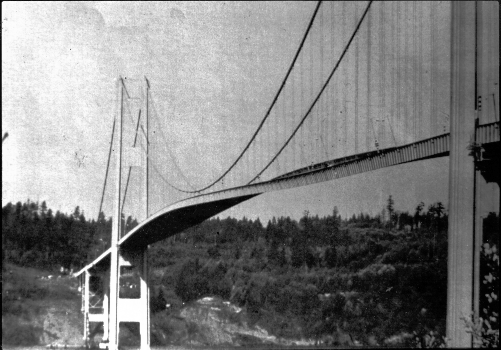
\includegraphics[height=.3\textwidth]{tac06.png}}
  \subfigure[Failure of the bridge]{
      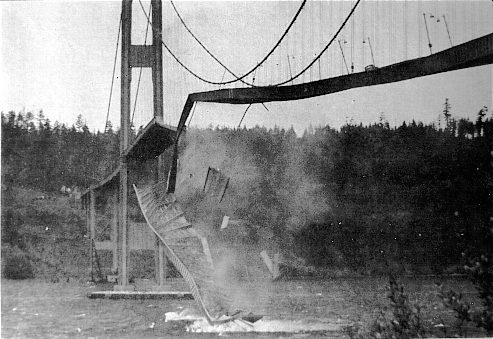
\includegraphics[height=.3\textwidth]{tac09.png}}
  \caption{Tacoma Narrows bridge flutter, from \citet{Smith1974}.}
  \label{fig:tacoma_bridge}
\end{figure}

Three vibration scenarios can appear, one leading to flutter.
The first scenario is the damped (or positively damped) 
vibration meaning
that the amplitude of the vibration decreases with respect to time, 
as shown in Fig.~\ref{fig:flutter_damped}.
This is the most wanted behavior as the system tends to
a stable point. In this case, the blade is said to
be flutter-free for the studied mode.
The second scenario is the amplified (or negatively damped)
vibration, namely flutter, shown in Fig.~\ref{fig:flutter_amplified}. 
This was the scenario that occurred on the Tacoma bridge. 
This scenario ultimately
leads to failure which is not acceptable. This is particularly true
on CROR configuration, as a blade failure might lead to 
the crash of the airplane as detailed in Sec.~\ref{sec:cror_challenges}.
The last scenario is the Limit Cycle Oscillation (LCO) vibration.
In this scenario, the deformation increases until a certain 
amplitude and then stays constant. This scenario is not
destructive by essence compared to the amplified scenario. However,
if the blade is repetitively excited by LCO, the blade
can fail as a consequence of structure fatigue.
\begin{figure}[htp]
  \centering
  \subfigure[damped (stable)]{
      \label{fig:flutter_damped}
      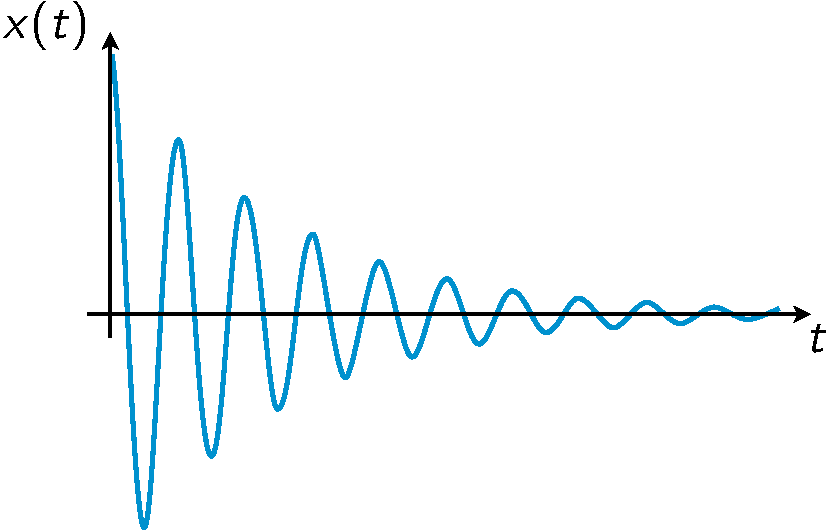
\includegraphics[width=.3\textwidth]{flutter_damped.pdf}}
  \subfigure[amplified (flutter)]{
      \label{fig:flutter_amplified}
      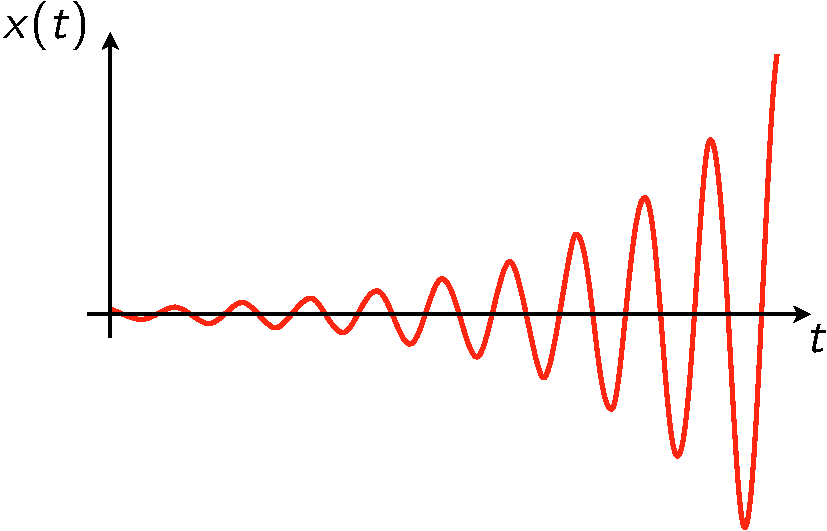
\includegraphics[width=.3\textwidth]{flutter_amplified.pdf}}
  \subfigure[Limit cycle oscillation]{
      \label{fig:LCO}
      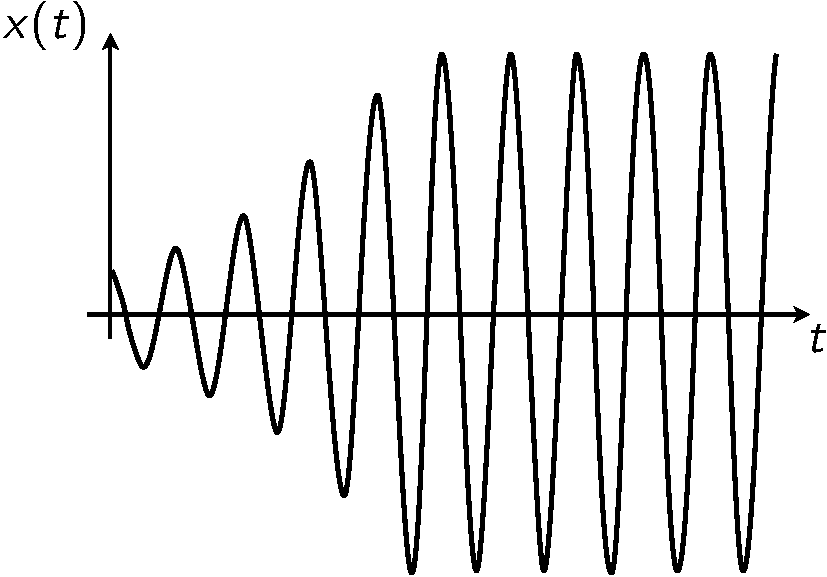
\includegraphics[width=.3\textwidth]{LCO.pdf}}
  \caption{Different vibration scenario for the flutter phenomenon.}
\end{figure}

The development of one scenario over another one is linked to
the fluid response to the vibration of the blade. In fact,
if the aerodynamic loads projected on the direction of the vibration
is positive, this means that the displacement will be amplified. 
In opposite, if the force is in opposed direction, the vibration will be damped.
The out-of-phase component of the aerodynamic force compared to
the displacement vector will give finally the sign of the aerodynamic damping.
The amplitude will give its strength. 

In this thesis, only the flutter boundary is assessed. In fact,
LCO can only be computed using a strong coupled fluid-structure 
approach and a weak coupling approach is chosen in this thesis
as detailed in the following Section.


\section{Computational AeroElasticity (CAE)}
\label{sec:ael_cae}
%!TEX root = ../../../adrien_gomar_phd.tex

Solving this equation analytically is generally 
not feasible. In fact, in turbomachinery, 
the flow exhibits non-linear features such as turbulence, shock and
boundary-layer interaction, to name but a few, that are out of reach for
analytical methods.

Two main strategies exist then for solving equation~\ref{eq:ael_motion_eq}:
the strong-coupling and the weak-coupling. The strong-coupling 
approach solves either the equation directly or two solvers are coupled and 
compute the aerodynamic and structural response of the system, respectively.
The strong coupling remains computationally expensive~\cite{Bartels2007}
and numerically stiff~\cite{Datta2008}.
It is therefore not used in this thesis.

In opposite, the weak-coupling approach has been widely used
in the turbomachinery aeroelasticity community~\cite{Marshall1996}.
This method uses a modal approach to identify the structural modes.
This modes are then prescribed with an harmonic motion in the aerodynamic
flow solver and the damping is computed.

To do so the aerodynamic force $F(t)$ and
the structural damping matrix $D$ are considered to be zero
and Eq.~\eqref{eq:ael_motion_eq} becomes:
\begin{equation}
	M \ddot{x}(t) + K x(t) = 0.
	\label{eq:ael_motion_eq_free_response}
\end{equation}
Considering now that the displacement vector $x(t)$ is harmonic
yields the eigen-value problem:
\begin{equation}
	\mdet \left(K - \omega^2 M  \right) = 0.
	\label{eq:ael_motion_eq_eigen_value}
\end{equation}
The solution of this equation are the modes $\psi_r$
and their frequency $\omega_r$, verifying:
\begin{equation}
	\left(K - \omega_r^2 M  \right) \psi_r = 0.
\end{equation}
The modes define a modal basis 
$\Psi = [\psi_0, \psi_1, \dots \psi_n]$.
Once the modal basis
is identified, either by mean of a Finite
Element model or an experimental identification, 
equation~\ref{eq:ael_motion_eq} becomes:
\begin{equation}
  \label{eq:2}
  M_m \ddot{q}(t) + D_m \dot{q}(t) + K_m q (t) - \Psi^\top F(t)=0, \quad x(t) = \Psi q(t).
\end{equation}
$M_m$, $D_m$ and $K_m$ are the modal mass, 
damping and stiffness, respectively.
The weak coupling approach assumes the linearity of the response of
the fluid with respect to the displacement of the structure. Therefore
small displacements are assumed and the so-called Generalized
Aerodynamic Forces (GAF) are linearized, which adds aerodynamic
stiffness~$K_A$ and damping~$D_A$:
\begin{equation}
  \label{eq:4}
  \Psi^\top F(t) = D_A\dot{q}(t) + K_A q(t).
\end{equation}
In order to estimate the unsteady aerodynamic forces $F(t)$, 
a fluid simulation is run with a prescribed harmonic motion of the
structure:
\begin{equation}
  \label{eq:6}
  q(t)=\cos(\omega t).
\end{equation}
A stability analysis is then performed in the frequency domain:
\begin{equation}
  \label{eq:5}
  q=\hat{q}e^{p t}\Rightarrow\left(
    p^2M + p(D-D_A) + (K-K_A)
  \right)\hat{q}=0,
\end{equation}
where the Laplace variable $p$ is of the form
$p=i\omega(1+i\alpha)$. Finally, considering only weakly damped or
amplified modes (i.e. $|\alpha| \ll 1$), the damping of the
fluid/structure coupled system reads $\alpha=-\Re e(p)/\Im m(p)$.

\subsection{Structural dynamics of turbomachinery blade}
\label{sub:structural_dynamics_of_turbomachinery_blade}

The modes are classified by their global shape: 
bending/flexion (noted F) and torsion (noted T) 
modes are the main ones. Then they are classified
depending on the number of deflection lines that they
have. If one deflection line is present in a flexion 
mode, it is called 1F and 2F if two deflection lines are
seen, as shown in Fig.~\ref{fig:blade_mode_shape}.
\begin{figure}[htp]
  \centering
  \includegraphics*[width=0.40\textwidth]{blade_mode_shape.pdf}
  \caption{Blade mode shape nomenclature.}
  \label{fig:blade_mode_shape}
\end{figure}




\chconclu{}

%!TEX root = ../../../adrien_gomar_phd.tex
\chapter{Fourier-based time methods}
\label{cha:spectral_methods}

\chabstract{The four main
Fourier-based time methods are presented in this chapter: the Linearized 
Unsteady Reynolds-averaged Navier--Stokes (LUR), 
the Non-Linear Harmonic (NLH), 
the Non-Linear Frequency Domain (NLFD) 
and the Harmonic Balance (HB) methods. The LUR
method comes from a linearization of the governing equations
while the three others are built to take into account for the 
non-linearities. The NLH, NLFD and HB methods
rely on a decomposition of the variable of interest
in Fourier series. By truncating these at order $N$,
$2N+1$ steady equations coupled by
a source term are obtained. 
Emphasis is put on the development
of the multi-frequential formulation and its
mathematical background to allow multi-frequential applications.
This is the case, for instance, of a pylon-rotor-rotor configuration
(namely an installed CROR) or a CROR with a moving blade, which is
the purpose of the current thesis.
The applicability of 
these methods is demonstrated in the literature
through analytical test cases, $2$D/$3$D academic 
turbomachine configurations,
industrial subsonic/transonic multi-stage applications, 
aeroelastic configurations and even unsteady
optimization problems proving their maturity. The cost of the methods
is almost $2N+1$ times the cost of a steady
computation with $N$ being the number of computed harmonics.
This thesis rely on the former work of \citet{ThesisSicot} who initially
implemented the harmonic balance method in the \textit{elsA}
code at CERFACS. Recently \citet{ThesisGuedeney} extended it to the
multi-frequential framework}

\minitoc
\newpage

% ================
% = INTRODUCTION =
% ================
\section{Introduction}
\label{sec:sm_intro}
%!TEX root = ../../adrien_gomar_phd.tex

The computational power available today in
the research centers and in the industry
is so big that large eddy simulation
becomes possible for some industrial configurations.
This is actually needed as high-fidelity
simulations help the turbomachinery community understand
the complex nature of flows that develop 
within these components,
allowing breakthrough ideas.
However, even if high fidelity approaches
are today within reach, it is still a challenge for
multi-row configurations.
Moreover, they will always be room for fast reliable
computations. 
As a matter of fact, on a daily basis, engineers need
to run lots of simulations to test new designs.
In this framework, large eddy simulation is
too demanding to be used for design purposes.

Today, in most companies, steady Reynolds-Averaged
Navier-Stokes (RANS) based solver are used on a daily basis.
For instance, this tool 
helped building the new $3$D-shape
of the forthcoming CFM-LEAP engine
depicted in Fig.~\ref{fig:sm_leap}.
\begin{figure}[htbp]
  \centering
  \includegraphics*[width=0.40\textwidth]{leap.jpg}
  \caption{$3$D-shape fan blades of the forthcoming CFM-LEAP engine.}
  \label{fig:sm_leap}
\end{figure}
Some further improvements are made possible by the use
of the unsteady RANS computations.
However, in the industry, unsteady computations
are still too expensive to be used on a daily basis.
Based on a simple idea, spectral methods are 
able to reproduce the unsteady field to engineering
accuracy, for a cost proportional to the cost of a
steady computation.

In turbomachines, the relative speed motion between the blades
give rise to inherent time-periodic phenomena.
In fact, consider a stage of a turbomachine, as for instance
a turbine stator-rotor configuration as shown 
in Fig.~\ref{fig:sm_unsteady_turbomachine}. 
\begin{figure}[htbp]
  \centering
  \includegraphics*[width=0.4\textwidth]{unsteady_turbomachine.pdf}
  \caption{Main unsteady effects present in a turbomachinery stage. Here, a turbine stator-rotor
  configuration is shown.}
  \label{fig:sm_unsteady_turbomachine}
\end{figure}
Due to the
viscosity effects acting on the stator blades, 
a wake is generated behind it and 
impinges the rotor row. In opposite, the flow field
generated around the rotor can literally go back up
to the stator row. In fact
the acoustic fluctuations can go backwards yielding
the potential effects. Moreover as, the rows have a 
rotation speed difference,
the field that is created in one row is perceived as unsteady in the opposite 
row frame of reference. This unsteadiness can be
correlated with the so-called Blade Passing Frequency (BPF) defined as:
\begin{equation}
	f = \frac{\Omega_{rel} B_{opp}}{2 \pi},
\end{equation}
where $f$ is the BPF, $\Omega_{rel}$ the relative speed difference 
and $B_{opp}$ the number of blades in the opposite row.
At first order, the unsteady effects presented here drive
most of the time-dependent field in a turbomachine. This 
is of course an approximation, but we will see at the end
of this chapter that the range of unsteady periodic
flow phenomenon in a CROR is large.

The problem with classical time-marching scheme is 
that it has no knowledge
of the periodic nature of the field yielding a time-consuming
transient. Thus, one idea is to build efficient algorithm
by taking advantage of this periodicity. 
Hence the spectral methods that are
presented above.



\section{The \texorpdfstring{\underline{L}}{L}inearized 
\texorpdfstring{\underline{U}}{U}nsteady 
\texorpdfstring{\underline{R}}{R}eynolds-averaged Navier--Stokes method (LUR)}
\label{sub:sm_lur}
%!TEX root = ../../../adrien_gomar_phd.tex

\citet{Verdon1984} originally developed the unsteady linearized 
method in the framework of potential flows. Later on, \citet{Hall1989}
extended it to the Euler equations and
\citet{Clark2000} applied it to the Reynolds-Averaged Navier--Stokes equations,
yielding the LUR method.
This method relies on a decomposition of the variables
into a base part (generally the steady-state) 
and a small-disturbance unsteady component
\begin{equation}
	u = \overline{u} + u^\prime,
	\label{eq:sm_lur_decomposition}
\end{equation}
where $u^\prime$ is considered to be a small unsteady perturbation.
In his PhD thesis,
\citet{Hall1987} defines small to be less than $10\%$ of the
steady flow.
Injecting Eq.~\eqref{eq:sm_lur_decomposition} into 
Eq.~\eqref{eq:sm_nonlinear_convection_conservative} yields
\begin{equation}
	\frac{\partial u^\prime}{\partial t} + 
	\frac{1}{2}\frac{\partial}{\partial x} \left[
	\overline{u}^2 + 2 \overline{u} u^\prime + u^\prime u^\prime \right] = 
	0.
	\label{eq:sm_lur_step_1}
\end{equation}
By means of linearization, \emph{i.e.} collecting terms
of equal order (equivalently $\overline{u^\prime} = 0$) 
and neglecting terms of order greater than one, 
Eq.~\eqref{eq:sm_lur_step_1} can be split
into a steady equation
\begin{equation}
	\frac{1}{2} \frac{\partial \overline{u}^2}{\partial x} = 0,
	\label{eq:sm_lur_step_2}
\end{equation}
and an unsteady first-order perturbation equation
\begin{equation}
	\frac{\partial u^\prime}{\partial t} +
	\frac{\partial}{\partial x} \left[
	\overline{u} u^\prime \right] = 
	0.
	\label{eq:sm_lur_step_3}
\end{equation}
There is a one-way coupling between the two equations:
the steady field
is first computed using Eq.~\eqref{eq:sm_lur_step_2}
and is secondly given as an input to the
perturbation equation to compute
the corresponding unsteady disturbance (Eq.~\eqref{eq:sm_lur_step_3}). 
However, the computed
perturbation is not used to update the steady solution.
Hence the one-way coupling.

\subsection{Mono-frequential formulation}
As mentioned before, Fourier-based time methods have been developed to efficiently
capture periodic phenomena.
Hence, assuming that the velocity perturbation is harmonic with 
angular frequency $\omega$, one can write
\begin{equation}
	u^\prime = \widehat{u}_1 e^{i \omega t} + \widehat{u}_{-1} e^{-i \omega t},
\end{equation}
with $\widehat{u}_1$ and $\widehat{u}_{-1}$ being complex conjugates giving a
real value for the perturbation.
Injecting this definition into Eq.~\eqref{eq:sm_lur_step_3} and using
the orthogonality property of the complex exponentials leads
to
\begin{equation}
	\begin{dcases}
		i \omega \widehat{u}_1 +
		\frac{\partial}{\partial x} \left[
		\overline{u} \widehat{u}_1 \right] &= 
		0, \\
		-i \omega \widehat{u}_{-1} +
		\frac{\partial}{\partial x} \left[
		\overline{u} \widehat{u}_{-1} \right] &= 
		0.
	\end{dcases}
	\label{eq:sm_lur_step_4}
\end{equation}
Finally a pseudo-time $\tau$ is added to time-march 
Eq.~\eqref{eq:sm_lur_step_2} and Eq.~\eqref{eq:sm_lur_step_4}
to the steady-state, giving three equations in total
\begin{alignat}{2}
	\fbox{$
	\begin{dcases}
		\frac{\partial \overline{u}}{\partial \tau} +
		\frac{\partial 
			\overline{u}^2}{\partial x} &= 0, \\
		\frac{\partial \widehat{u}_1}{\partial \tau} +
		i \omega \widehat{u}_1 +
			\frac{\partial}{\partial x} \left[
			\overline{u} \widehat{u}_1 \right] &= 
			0, \\
		\frac{\partial \widehat{u}_{-1}}{\partial \tau}
		-i \omega \widehat{u}_{-1} +
			\frac{\partial}{\partial x} \left[
			\overline{u} \widehat{u}_{-1} \right] &= 
			0
	\end{dcases}
	$}
\end{alignat}

\subsection{Extension to the Navier--Stokes equations}
To extend the LUR method to the Reynolds-Averaged
Navier--Stokes equations, one has to consider
their linearized counterpart.
The reader is referred to the paper of \citet{Clark2000} for
a detailed development of the LUR method for the Navier--Stokes
equations.

\subsection{Numerical cost}
As the method is based on three equations in total, one steady equation 
(namely a classical RANS equation) and two perturbation equations, 
if $\mathdollar_{\text{RANS}}$ 
denotes the CPU and memory cost of
one steady computation, then the cost of the LUR
method can be estimated as
\begin{equation}
	\mathdollar_{\text{LUR}} = 3 \times \mathdollar_{\text{RANS}}.
\end{equation}
In practice, only two computations are performed since the steady computation
is usually available beforehand.


\section{The \texorpdfstring{\underline{N}}{N}on-\texorpdfstring{\underline{L}}{L}inear 
\texorpdfstring{\underline{H}}{H}armonic method (NLH)}
\label{sub:sm_nlh}
%!TEX root = ../../../adrien_gomar_phd.tex

Originally developed by \citet{He1998} and \citet{Ning1998},
the NLH method
relies on a decomposition of the conservative variables into a
time-averaged part plus an unsteady perturbation
\begin{equation}
	u = \overline{u} + u^\prime,
	\label{eq:sm_nlh_decomposition}
\end{equation}
where $\overline{\vphantom{u}.}$ denotes the time-averaging operator and
$.^\prime$ its unsteady perturbation counterpart.
By injecting Eq.~\eqref{eq:sm_nlh_decomposition} into
Eq.~\eqref{eq:sm_nonlinear_convection_conservative}, one gets
\begin{equation}
	\frac{\partial u^\prime}{\partial t} + 
	\frac{1}{2}\frac{\partial}{\partial x} \left[
	\overline{u}^2 + 2 \overline{u} u^\prime + u^\prime u^\prime \right] = 
	0.
	\label{eq:sm_nlh_step_1}
\end{equation}
The equation for the time-averaged part can be obtained by time-averaging
equation~\eqref{eq:sm_nlh_step_1}
\begin{equation}
	\frac{\partial}{\partial x}
	\left[\overline{u}^2 + 
	\overline{u^\prime u^\prime}\right] =
	0,
	\label{eq:sm_nlh_step_2}
\end{equation}
The term $\overline{u^\prime u^\prime}$
accounts for the non-linearities of the considered equations. 
This term reflects the influence of the unsteady contribution to
the time-average, which was neglected in the LUR approach. It
is called the non-linear 
(or the deterministic) stress terms, by analogy with
the Reynolds stress terms. 
The equation for the unsteady perturbation is then obtained by keeping
the first-order terms of the unsteady equation~\eqref{eq:sm_nlh_step_1}.
This means that the term $u^\prime u^\prime$ is neglected, yields
\begin{equation}
	\frac{\partial u^\prime}{\partial t} + 
	\frac{\partial}{\partial x} \left[\overline{u} u^\prime \right] = 
	0.
	\label{eq:sm_nlh_step_3}
\end{equation}
Note that neglecting the high-order terms 
(namely $u^\prime u^\prime$ for the Burger's equation) 
is almost similar to
linearizing the equation. However, in the NLH approach,
the time-averaged $\overline{u^\prime u^\prime}$ 
of $u^\prime u^\prime$ is kept in
equation~\eqref{eq:sm_nlh_step_2} which accounts for a part of the
non-linearities. Thus, the method is not linear. Equations~\eqref{eq:sm_nlh_step_2} 
and~\eqref{eq:sm_nlh_step_3} 
are simultaneously solved, leading to a two-way coupling.

\subsection{Mono-frequential formulation}
Up to now, no assumption has been made neither on the velocity $u$,
nor on its time-averaged part or unsteady perturbation part.
Assuming now that the velocity perturbation 
is periodic in time with period
$T=2 \pi / \omega$,
the unsteady perturbation can be decomposed into 
a Fourier series
\begin{equation}
	u^\prime = \sum_{\genfrac{}{}{0pt}{}{k=-\infty}{k \neq 0}}^{\infty} 
	\widehat{u}_k e^{i \omega k t},
	\label{eq:sm_nlh_decomposition_pert}
\end{equation}
where the $k=0$ term is omitted as it is accounted for in
the $\overline{u}$ part.
The complex exponentials family forming
an orthogonal basis, we retrieve for all harmonics 
$-\infty \leq k \leq \infty, \; k \neq 0$
\begin{equation}
	i \omega k \widehat{u}_k + 
	\frac{\partial}{\partial x} \left[ \overline{u} \widehat{u}_k\right] =
	0,~\forall k.
	\label{eq:sm_nlh_decomposition_pert_part1}
\end{equation}
Each one of harmonic equation~\eqref{eq:sm_nlh_decomposition_pert_part1}
represents now a steady-flow-like equation as no temporal
derivative is present anymore.

The term $\overline{u^\prime u^\prime}$ remains in the time-averaged
equation~\eqref{eq:sm_nlh_step_2}
and needs to be computed. It can be 
directly worked out when the harmonics are known 
from Eq.~\eqref{eq:sm_nlh_decomposition_pert_part1}
\begin{equation}
	\begin{split}
		u^\prime u^\prime &= 
		\left[
			\sum_{\genfrac{}{}{0pt}{}{k=-\infty}{k \neq 0}}^{\infty} \widehat{u}_k e^{i \omega k t} 
		\right]
		\left[
			\sum_{\genfrac{}{}{0pt}{}{k=-\infty}{k \neq 0}}^{\infty} \widehat{u}_k e^{i \omega k t} 
		\right] \\
		&= \sum_{\genfrac{}{}{0pt}{}{k=-\infty}{k \neq 0}}^{\infty} (\widehat{u}_k)^2
		   e^{i 2 \omega k t} +
		   2 \sum_{\genfrac{}{}{0pt}{}{k,j=-\infty}{k \neq j \neq 0}}^{\infty} 
		   \widehat{u}_k \widehat{u}_j e^{i \omega (k + j) t}.
	\end{split}
\end{equation}
Thus, the time-average becomes
\begin{equation}
	\begin{split}
		\overline{u^\prime u^\prime} &= 
		\frac{1}{T} \int_{t=0}^{T} \left[ 
			\sum_{\genfrac{}{}{0pt}{}{k=-\infty}{k \neq 0}}^{\infty} (\widehat{u}_k)^2
		   	e^{i 2 \omega k t} +
		   	2 \sum_{\genfrac{}{}{0pt}{}{k,j=-\infty}{k \neq j \neq 0}}^{\infty} 
		   	\widehat{u}_k \widehat{u}_j e^{i \omega (k + j) t} 
		\right] \diff t\\
		&= \frac{2}{T} \int_{t=0}^{T} \sum_{\genfrac{}{}{0pt}{}{k,j=-\infty}{k \neq j \neq 0}}^{\infty} 
		   	\widehat{u}_k \widehat{u}_j 
		   	e^{i \omega (k + j) t} \diff t \\
		&= \frac{2}{T} \int_{t=0}^{T} 
			\sum_{\genfrac{}{}{0pt}{}{k=-\infty}{k \neq 0}}^{\infty} 
			\widehat{u}_k \widehat{u}_{-k}  \diff t.
	\end{split}
\end{equation}
As $\widehat{u}_k$ and $\widehat{u}_{-k}$ are complex conjugates,
$\overline{u^\prime u^\prime}$ is finally equal to
\begin{equation}
	\overline{u^\prime u^\prime} = 
	2 \sum_{\genfrac{}{}{0pt}{}{k=-\infty}{k \neq 0}}^{\infty} |\widehat{u}_k|^2.
	\label{eq:sm_nlh_deterministic_stress_terms}
\end{equation}
This last equation depends only on the computed harmonics, meaning
that no term is modeled. Moreover, this term couples the
time-average solution with the unsteady perturbation
and takes into account for a part of the 
non-linearities of the considered equation, which makes a
great difference with the approach of Sec.~\ref{sub:sm_lur}.

Finally, as computing an infinite number of harmonics is 
numerically not feasible,
it is truncated at order $N$. 
This is a fair assumption as most
of the physical flows have a finite unsteady spectrum.
Moreover, the goal of Fourier-based time
methods is to have a compact representation of the unsteady time
signals.
As for a mesh grid convergence, the number of harmonics $N$
will directly impact the accuracy of the unsteady representation
of the signal.
The discussion on the
convergence of Fourier-based time methods will be introduced mathematically
in Sec.~\ref{sec:spectral_accuracy} and discussed later on in this 
thesis in Chap.~\ref{cha:limitations_convergence}.

To summarize, the NLH
method applied to Eq.~\eqref{eq:sm_nonlinear_convection_conservative}
gives $2N$ perturbation equations and one time
averaged equation making $2N+1$ equations in total. 
A pseudo-time ($\tau$) derivative is
added to march the equations in pseudo-time to the steady-state 
solution of all the harmonics
\begin{equation}
	\fbox{$
	\begin{dcases}
		\frac{\partial \overline{u}}{\partial \tau} + 
		\frac{\partial}{\partial x}
			\left[\overline{u}^2 + 
			\overline{u^\prime u^\prime}\right] &=
			0, \\
		\frac{\partial \widehat{u}_k}{\partial \tau} + 
		i \omega k \widehat{u}_k + 
			\frac{\partial}{\partial x} 
			\left[ \overline{u} \widehat{u}_k\right] &= 
			0, \: k \in [-N, N], \: k \neq 0
	\end{dcases}
	$}
	\label{eq:sm_nlh_subset_eq}
\end{equation}
The equations are coupled by the deterministic 
stress term $\overline{u^\prime u^\prime}$
defined in Eq.~\eqref{eq:sm_nlh_deterministic_stress_terms}.
The term $u^\prime u^\prime$ is neglected in this formulation.

\subsection{Multi-frequential formulation}

\citet{He2002} extended the method to a multi-frequential
formulation. Instead of writing the perturbation
using a Fourier series as defined in Eq.~\eqref{eq:sm_nlh_decomposition_pert},
it is written using a sum of harmonics each of which
having an angular frequency $\omega_k$
\begin{equation}
	u^\prime = \sum_{\genfrac{}{}{0pt}{}{k=-N}{k \neq 0}}^{N} 
	\widehat{u}_k e^{i \omega_k t}.
	\label{eq:sm_nlh_decomposition_pert_multi}
\end{equation}
Note that the term $k \omega$ in Eq.~\eqref{eq:sm_nlh_decomposition_pert}
is now replaced by $\omega_k$ meaning that the frequencies can be chosen
arbitrarily.
The derivation of the equations is kept the same and the following
$2N+1$ subset of equations is finally obtained
\begin{equation}
	\fbox{$
	\begin{dcases}
		\frac{\partial \overline{u}}{\partial \tau} +
		\frac{\partial}{\partial x}
			\left[\overline{u}^2 + 
			\overline{u^\prime u^\prime}\right] &=
			0, \\
		\frac{\partial \widehat{u}_k}{\partial \tau} + 
		i \omega_k \widehat{u}_k + 
			\frac{\partial}{\partial x} 
			\left[ \overline{u} \widehat{u}_k\right] &= 
			0, \: k \in [-N, N], \: k \neq 0
	\end{dcases}
	$}
	\label{eq:sm_nlh_subset_eq_multi}
\end{equation}
However, as the complex exponentials 
($e^{i \omega_k t}$) do not form
an orthogonal basis, writing Eq.~\eqref{eq:sm_nlh_subset_eq_multi}
for each harmonic $k \in [-N, N], \: k \neq 0$ is mathematically
not true. \citet{He2002} argued that the terms
are collected for each harmonic. 
The same development is made by \citet{Vilmin2006}.

The coupling deterministic stress term is evaluated using the
same equation as for the mono-frequential formulation
\begin{equation}
	\overline{u^\prime u^\prime} = 
	2 \sum_{\genfrac{}{}{0pt}{}{k=-\infty}{k \neq 0}}^{\infty} |\widehat{u}_k|^2.
	\label{eq:sm_nlh_deterministic_stress_terms2}
\end{equation}
To give a mathematical framework to prove this assertion, 
let us consider the specific example of $u^\prime$ taken as
\begin{equation}
	u^\prime = (\widehat{u}_{-1} e^{-i t} + \widehat{u}_{1} e^{i t}) +
		(\widehat{u}_{-2} e^{-i \pi t} + \widehat{u}_{2} e^{i \pi t}),
\end{equation}
namely, we consider equation~\eqref{eq:sm_nlh_decomposition_pert_multi}
with the specific angular frequencies: $\omega_1 = 1$ and $\omega_2 = \pi$.
The cross-term $u^\prime u^\prime$ is then equal to
\begin{equation}
	\begin{split}
		u^\prime u^\prime = 
			&(\widehat{u}_{-1})^2 e^{-i 2 t}
			+ (\widehat{u}_{1})^2 e^{i 2 t}
			+ (\widehat{u}_{-2})^2 e^{- i 2 \pi t}
			+ (\widehat{u}_{2})^2 e^{i 2 \pi t} \\
		&+ 2 \left[
				\widehat{u}_{-1} \widehat{u}_{-2} e^{i (-1 -\pi) t} 
				+ \widehat{u}_{-1} \widehat{u}_{2} e^{i (-1 + \pi) t}
				+ \widehat{u}_{1} \widehat{u}_{-2} e^{i (1 - \pi) t} 
				+ \widehat{u}_{1} \widehat{u}_{2} e^{i (1 + \pi) t} 
			 \right] \\
		&+ 2 \widehat{u}_{-1}\widehat{u}_{1}
			 	+ 2 \widehat{u}_{-2}\widehat{u}_{2}.
	\end{split}
\end{equation}
In the mono-frequential framework, the frequencies are harmonically related
and a common period $T$ exists. This logically leads to the definition
of the mean value $\overline{f}$ of such a time-varying function $f(t)$ as
\begin{equation}
	\overline{f} = \frac{1}{T} \int_0^T f(t) \diff t.
\end{equation}
In the current multi-frequential example, 
$\pi$ and $1$ are not integer multiples of a common fundamental
frequency. Therefore, a common period $T$ does
not necessarily exist. \citet{Besicovitch1932}
defines a mathematical framework for such functions. In this framework
the temporal mean value exists and is defined as
\begin{equation}
	\overline{f} = \lim_{X \to \infty} \frac{1}{X} \int_0^X f(t) \diff t.
\end{equation}
The mean value of the cross-term $u^\prime u^\prime$ is thus equal to
\begin{equation}
	\overline{u^\prime u^\prime} = 2 (\widehat{u}_{-1}\widehat{u}_{1} + 
		\widehat{u}_{-2}\widehat{u}_{2}) = 2 (|\widehat{u}_1|^2 + |\widehat{u}_2|^2),
\end{equation}
as the mean value of purely harmonic functions is zero.
Extending this demonstration to the arbitrary case of a
multi-frequential perturbation 
(Eq.~\eqref{eq:sm_nlh_decomposition_pert_multi}) leads to
the general expression given in equation~\eqref{eq:sm_nlh_deterministic_stress_terms2}.


\subsection{Extensions}

\paragraph{Navier--Stokes equations}
As shown above, since the development of the NLH
method is made in the frequency domain, applying the method to
complex equations can be difficult. For the Navier--Stokes equations,
this step is tedious due to the number of equations to treat. Nevertheless, 
\citet{He1998, Chen2001, He2002} and \citet{Vilmin2006} have
done this and the reader is referred to these papers
for a detailed description.
Note that in all those publications, turbulence is modeled
using only the time-averaged quantities.
This is another assumption as the turbulent field, in a wake
for instance, is seen unsteady in the opposite row frame
of reference~\cite{Lakshminarayana1980}. Thus, this
unsteadiness is not taken into account by the NLH method.

\paragraph{Turbomachinery computations}
Originally, the NLH method has been developed for 
turbomachinery applications. \citet{He1998} and
\citet{Ning1998} computed isolated turbomachinery
configurations. To reduce the domain to a single 
blade-to-blade passage, they consider a periodic
boundary condition for the time-averaged part and a
phase-lagged boundary condition for the perturbation part on the
azimuthal boundaries
\begin{equation}
    \begin{split}
    	\overline{u}_U &= \overline{u}_L, \\
    	u^\prime_U &= u^\prime_L e^{i \sigma},
    \end{split}
\end{equation}
where subscripts $U$ and $L$ denote 
the upper and the lower boundaries, respectively, and $\sigma$ is the
inter-blade phase angle. This allows to compute
isolated vibrating configurations thanks to 
the phase theorem of \citet{Lane1956} (see Sec.~\ref{sub:lane_theorem}).

\citet{Chen2001} added a rotor-stator treatment
to allow the computation of stage configurations. 
To do so, the perturbation 
$u^\prime$ is exchanged at the interface using
an azimuthal Fourier transform, whereas
the time-average field $\overline{u}$ 
and the deterministic stresses 
$\overline{u^\prime u^\prime}$
are azimuthally flux-averaged.
To this aim, the azimuthal variations of 
the perturbation $\widehat{u} (\theta_i)$
are spatially Fourier transformed ($\widetilde{u}_i$)
and exchanged at the interface 
($\widetilde{u}_i = \widetilde{u}_j$). Subscript $i$ and $j$ denotes,
respectively, the upstream and the downstream rows.
This is schematically represented in 
Fig.~\ref{fig:bnd_sliding_chen2001}.
\begin{figure}[htp]
  \centering
  \includegraphics*[scale=0.25]{bnd_sliding_chen2001.pdf}
  \caption{Exchange of the variables at rows interface as described by \citet{Chen2001}.}
  \label{fig:bnd_sliding_chen2001}
\end{figure}

Still the method is restricted to mono-frequential problems, since only
one stage is considered, each row seeing the
opposite blade passing frequency. Considering
the time-averaged field to be constant in the azimuthal 
direction at the interface seems fair (in case 
without clocking effects), 
but there is
no reason for $\overline{u^\prime u^\prime}$ to be so.
\citet{He2002} extended the method to take into
account multi-stage configurations through the
development of a multi-frequential formulation.
In fact, in such an application, 
a sandwiched row will see unsteadinesses coming
from the upstream row (mainly wake effects) and
potential effects from the downstream rows. In the
general case where the surrounding rows do not have the
same blade passing frequencies, multiple frequencies
can be present in the current row.
The same treatment is used at the rows interfaces meaning
that the time-averaged quantities are flux-averaged and the
fluctuations are exchanged through their azimuthal
Fourier transform.
\citet{Vilmin2006} extended the rotor-stator
interface to a non-matching join sliding mesh interface which
leads to the continuity of the unsteady flow field at the interface.
The main difference with the previous treatment is that
$\overline{u}$ and $\overline{u^\prime u^\prime}$ 
are not flux-averaged but rather spatially Fourier transformed,
which leads to the continuity of $u$ at the interface, when
the number of harmonics is sufficient.

\paragraph{Clocking effect}
\citet{He2002} extended the NLH method to
the computation of all clocking positions in one computation.
\begin{figure}[htp]
  \centering 
  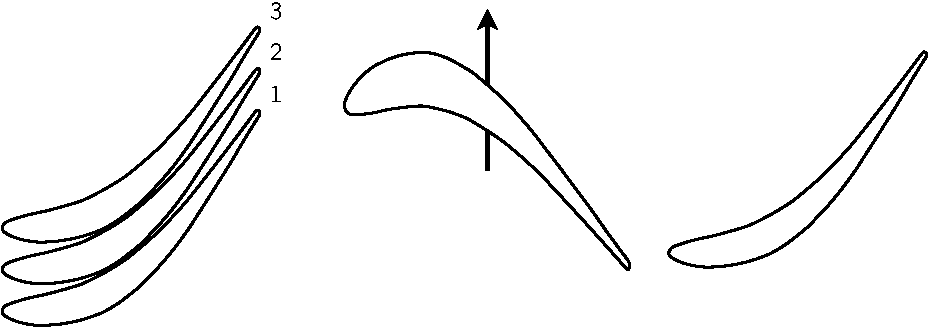
\includegraphics[width=.5\textwidth]{clocking_effect.pdf}
  \caption{Different clocking positions for a stator/rotor/stator
  configuration.}
  \label{fig:sm_nlh_clocking_effect}
\end{figure}
Fig.~\ref{fig:sm_nlh_clocking_effect} shows three
different clocking positions (sometimes also referred 
to as the indexing positions)
of the first stator
in a stator/rotor/stator configuration. In this figure,
the first clocking position is aligned with the second stator.
The second and the third clocking positions are not aligned with
the second stator, which may give different level of perceived
unsteadiness by the second stator. At a design phase, the engineer can choose any
relative position of the rows and thus any clocking position.
The relative position of both stator is of
prior interest to choose the best clocking position. 
In fact, the wakes that are shed behind the first stator
are cut by the rotor blades and transmitted to 
the second stator row. The stators being fixed, the wake of
the first stator is seen as a stationary wave in the second stator.
Hence, the importance of their relative position. For instance,
\citet{Huber1996} showed that
on their 1.5 stage turbine, the variation of efficiency due to clocking
position was equal to $0.8\%$ of efficiency points, showing the
importance of the clocking effect.

The brute force approach to compute the clocking effect on a
configuration is to consider all the relative positions. This means
that the geometry of the stator should be rotated for each new 
clocking position and hence a new unsteady computation should be 
run. The innovative procedure proposed by 
\citet{He2002} is to consider the clocking effect as a steady wave.
In fact, as both stator are fixed, a steady perturbation
shed behind the first stator is still steady in the second stator.
In terms of frequencies, a steady perturbation
can be assimilated to a zero frequency mode. 
In \citet{He2002} and \citet{Vilmin2009}, 
a perturbation with a zero frequency
is thus additionally computed. The clocking effect can then be evaluated by
post-processing the Fourier coefficient of the zeroth frequency mode.
Recently, the computation of clocking effects on
arbitrary configurations has been made possible
by \citet{Vilmin2013a}. This allows its use for 
pylon-rotor-rotor applications for instance, which
is the configuration encountered in an installed CROR.

\subsection{Numerical cost}
Compared to the LUR method, the number of equations to solve is 
not constant here. In fact, if $N$ denotes the number of harmonics
computed in total (sum of each harmonic of each perturbation)
and if $\mathdollar_{\text{RANS}}$ 
denotes the CPU and memory cost of
one steady computation, $2N$ harmonic equations and 
one time-average equation
are solved, thus
\begin{equation}
	\mathdollar_{\text{NLH}} = (2N+1) \times \mathdollar_{\text{RANS}}.
\end{equation}
However, \citet{Vilmin2006} do not apply the NLH formulation
to the turbulent equation (in their case, 
the one equation of \citet{Spalart1992}). Therefore,
as only five equations are solved using the NLH approach, the 
turbulent equation being solved as a steady one,
the cost becomes
\begin{equation}
	\mathdollar_{\text{NLH}} = \frac{5 \times (2N+1) + 1}{6} \times \mathdollar_{\text{RANS}}.
\end{equation}



\section{The \texorpdfstring{\underline{N}}{N}on-\texorpdfstring{\underline{L}}{L}inear 
\texorpdfstring{\underline{F}}{F}requency \texorpdfstring{\underline{D}}{D}omain method (NLFD)}
\label{sub:sm_nlfd}
%!TEX root = ../../../adrien_gomar_phd.tex

\subsection{Mono-frequential formulation}

Originally proposed by \citet{McMullen2001}, the NLFD
method relies on a simple observation: to develop Fourier-based methods, and in
particular the NLH method, one has made use of the Fourier
series to efficiently represent an unsteady signal.
This representation has then be used to develop the unsteady
equation into $2N+1$ steady equations: one time-averaged equation
and $2N$ perturbation equations, 
where $N$ denotes the number
of harmonic kept to compute the solution.
The problem is that the equations need to be 
resolved in the frequency domain meaning
that all the numerical techniques should be adapted: the numerical schemes,
the turbulent models and so on. The (smart) idea 
proposed by \citet{McMullen2001} is to
make use of the fast Fourier Transform and its inverse to
allow an easy implementation of the method into a classical time-domain code.
To explain the development of this method, let us first 
write Eq.~\eqref{eq:sm_nonlinear_convection_conservative} 
in a more general form:
\begin{equation}
	(\ref{eq:sm_nonlinear_convection_conservative})
	\Leftrightarrow
	\frac{\partial u}{\partial t} + R = 0,
	\label{eq:sm_nonlinear_convection_residual}
\end{equation}
with
\begin{equation}
	R = \frac{\partial}{\partial x} \left( 
	\frac{u^2}{2} \right).
\end{equation}
Let us now consider that both $u$ and $R$ are periodic
in time with respect to period $T = 2 \pi / \omega$
and can be written using a Fourier series:
\begin{equation}
	\begin{split}
		u(t) &= \sum_{k=-\infty}^{\infty} \widehat{u}_k e^{i k \omega t}, \\
		R(t) &= \sum_{k=-\infty}^{\infty} \widehat{R}_k e^{i k \omega t}.
	\end{split}
\end{equation}
Note that decomposing $R(t)$ into a Fourier series is equivalent
to use the Fourier decomposition of $u(t)$ and express
$R(t)$ using the Fourier coefficients $\widehat{u}_k$ of $u$
since the cross-terms that may arise are also expressed 
using the same complex exponentials. This comes from the fact
that multiplying a complex exponential with a complex exponential
just forms a new complex exponential at the power of the sum of the
two.
Injecting these decompositions into 
Eq.~\eqref{eq:sm_nonlinear_convection_residual} and taking into account
for the orthogonality of the complex exponentials:
\begin{equation}
	i k \omega \widehat{u}_k + \widehat{R}_k = 0, \: k \in [-\infty, \infty].
\end{equation}
As previously, only a small number of harmonics $N$ is kept and 
a pseudo-time ($\tau$) derivative is added to march the equations
in pseudo-time to the steady-state solutions of all the harmonics:
\begin{equation}
	\fbox{$
	\displaystyle \frac{\partial \widehat{u}_k}{\partial \tau} + 
	i k \omega \widehat{u}_k + \widehat{R}_k = 0, \: k \in [-N, N].
	$}
	\label{eq:sm_nlfd_subset_eq}
\end{equation}
The fact that $R(t)$ is expressed using its own Fourier series 
makes it simpler to implement 
as it avoids developing its expression using 
the complex coefficients $\widehat{u}_k$. 
However, $\widehat{R}_k$ must be evaluated. To do so, as depicted
in Fig.~\ref{fig:nlfd_principle}, \citet{McMullen2001}
propose to use an Inverse Fast-Fourier Transform (IFFT) to get
$u(t)$ from $\widehat{u}_k$. Then the considered governing equations
are used to evaluate $R(t)$ which leads to $\widehat{R}_k$
through a Fast-Fourier Transform (FFT). Finally, the next iteration value 
$\widehat{u}_k$
is evaluated by adding $\widehat{R}_k$ and 
the corresponding temporal derivative $i k \omega \widehat{u}_k$. All
harmonics are coupled through the IFFT and FFT operations
that needs all of the former to compute the counterpart temporal signal,
hence the coupling. Moreover, 
in the non-viscous Burger's equation framework, 
the term $u^\prime u^\prime$ is not neglected anymore compared to the
NLH approach and the computation of the deterministic stress is encompassed
by the FFT and IFFT operations.
\begin{figure}[htbp]
  \centering
  \includegraphics*[width=0.50\textwidth]{nlfd_principle.pdf}
  \caption{Simplified diagram of the computation of $\widehat{R}_k$ from $\widehat{u}_k$
  for the non-linear frequency domain method.}
  \label{fig:nlfd_principle}
\end{figure}

\subsection{Extensions}

\paragraph{Navier--Stokes equations}
The Navier--Stokes equations can be written in finite-volume,
semi-discrete form as:
\begin{equation}
	V \frac{\partial W}{\partial t} + R(W) = 0,
	\label{eq:navier_stokes_fv_sd}
\end{equation}
where $V$ is the volume of the cell and $W$
the vector of conservative variables.
This formulation is similar to
Eq.~\eqref{eq:sm_nonlinear_convection_residual} meaning that
nothing particular has to be made to derive this approach for
the Navier--Stokes equations. This is indeed attractive as the
method can be applied almost directly, except for the FFT and IFFT
step that should be added into the pseudo time loop.

\paragraph{Aeroelastic computations}
Since both the structural and the aerodynamic equations
are prone to time-periodic unsteadinesses,
\citet{Kachra2008} extended the NLFD approach to the strong coupling of
aeroelasticity within the two-dimensional Euler equations framework.
Both the fluid dynamics and the structural equations
are solved using the NLFD approach. They are coupled together 
every $15$ multigrid cycles.
A $2$D plunging and pitching airfoil is considered.
They demonstrate that with a one-harmonic NLFD computation the
flutter boundary of a NACA$64A010$ airfoil is correctly predicted.
This leads to a gain of one order of magnitude compared to a classical
time-marching procedure. 

\paragraph{Gradient-based method to determine the frequency}
\citet{McMullen2001} applied the NLFD to a cylinder
vortex shedding. This could be done as the frequency of the
vortex shedding was known \emph{a priori} from experimental
and numerical data. Note that this supposes that the
numerical and the experimental vortex shedding frequencies
are equal, which is generally not true~\cite{Kato1991}.
However, for a given cylinder, it is generally not
possible to know this frequency \emph{a priori}. This is why
\citet{McMullen2002, McMullen2006a}
proposed a gradient based method for determining the frequency
of a periodic phenomena where the frequency is unknown
\emph{a priori}. They argue that the frequency domain formulation
helps forming a gradient operator to find the period $T$ based
on the minimization of the residual of the unsteady equations.
They applied their algorithm to find the frequency of the vortex
shedding around a cylinder, and found it with a $3.5\%$ accuracy
compared to experimental data. Nevertheless, as a gradient method is 
used, a good initial guess is needed for the algorithm to
converge. This limits the methods to well-known unsteady
problems. Moreover, the prior interest of the NLFD method is
to reduce the cost compared to a classical time-marching scheme
to solve the unsteady periodic problem. One may ask
if applying the NLFD with an gradient based method is not finally
more costly than a classical time-marching scheme.

\paragraph{Optimum shape design}
\citet{Nadarajah2003} compared an optimum shape design 
strategy for pitching airfoils 
using both a classical time-marching scheme
and the NLFD scheme within the Euler equations
framework. It is shown that the NLFD method
gives the same accuracy for the gradient and the optimum with only 
three time-instants (namely $N=1$)
compared to $23$ time-instants needed for 
the time-marching approach.
\citet{Nadarajah2007} extended it
to the three-dimensional Navier--Stokes equations.
A wing undergoing a change 
in angle of attack as a function of time is computed and
it is demonstrated that
five instants (namely $N=2$) is sufficient to provide
accurate results.
\citet{Tatossian2011} applied it
to the aerodynamic shape optimization of hovering rotor blades
in the Euler framework.
The capability of 
their shape optimization process
to redesign the Caradonna–Tung experimental 
blade is assessed and gives a proof
of concept.

\paragraph{Adaptive method}
The problem of Fourier-based methods is that the higher
the number of harmonics computed, the higher the corresponding
CPU and memory cost. There is thus a need to optimize
the chosen number of harmonics.
\citet{Mosahebi2013} implemented an adaptive NLFD approach named
the p-NLFD. Based on the energy of the last mode compared
to the whole spectrum, the number of harmonics
is increased if a fixed threshold is not reached.
A speed-up of $2$ in terms of CPU cost and
memory reduction is observed for the case of a
vortex-shedding behind a cylinder.

\subsection{Cost of the method}
The NLFD method is close to the NLH approach in terms of number
of equations solved. However, at each time-step a fast Fourier transform
is performed to cast back the harmonics into the time-domain in order
to compute the residual $R(t)$. \citet{McMullen2006} argue
that the cost of the fast Fourier transform is less than the cost of 
the spatial derivatives. 
\citet{Kachra2008} quantitatively estimate it to be
approximately $2\%$ of the cost of one iteration, which is negligible.
Based on this affirmation, one can say that 
if $\mathdollar_{\text{RANS}}$ 
denotes the CPU and memory cost of
one steady computation, the cost of the NLFD method can be 
approximated by:
\begin{equation}
	\mathdollar_{\text{NLFD}} = (2N+1) \times \mathdollar_{\text{RANS}}.
\end{equation}
This evaluation of the cost is confirmed by numerical
simulations by \citet{McMullen2002}.

% ====================
% = HARMONIC BALANCE =
% ====================
\section{The \texorpdfstring{\underline{H}}{H}armonic \texorpdfstring{\underline{B}}{B}alance method (HB)}
\label{sec:sm_hb}
%!TEX root = ../../../adrien_gomar_phd.tex

The HB method has been originally
proposed by \citet{Hall2002}, at that time named
Harmonic Balance Technique (HBT).
It can be considered as an improvement of the NLFD
approach. In fact, instead
of using the fast Fourier transform to cast back the equations
to the time domain at each pseudo-iteration step, 
the equations are mathematically derived to be directly
computed into the time-domain.
To explain the method, we will again use the general form of 
the non-viscous Burger's equation as defined in
Eq.~\eqref{eq:sm_nonlinear_convection_residual}.
This thesis rely on the former work of \citet{ThesisSicot} who
implemented the harmonic balance method into the 
\textit{elsA}~\cite{Cambier2013} CFD code at CERFACS. 
Recently \citet{ThesisGuedeney} extended it to the
multi-frequential formulation, allowing contra-rotating
open rotor aeroelastic computations. This is why this
approach will be used in the current PhD work.

\subsection{Mono-frequential formulation}

Following the same approach as the non-linear frequency domain one,
it is considered that both $u$ and $R$ are periodic
in time with respect to period $T = 2 \pi / \omega$
and can be written using Fourier series:
\begin{equation}
	\begin{split}
		u(t) &= \sum_{k=-\infty}^{\infty} \widehat{u}_k e^{i k \omega t}, \\
		R(t) &= \sum_{k=-\infty}^{\infty} \widehat{R}_k e^{i k \omega t}.
		\label{eq:sm_hall_dft}
	\end{split}
\end{equation}
Injecting Eq.~\eqref{eq:sm_hall_dft} in 
Eq.~\eqref{eq:sm_nonlinear_convection_residual}, and considering
the orthogonality of the complex exponentials:
\begin{equation}
	i k \omega \widehat{u}_k + \widehat{R}_k = 0, \: k \in [-N, N].
	\label{eq:sm_hall_frequential_eq}
\end{equation}

In the same way as one uses Fourier coefficients to
evaluate the temporal signal,
one can reconstruct the Fourier coefficients using
temporal evaluations. These are taken at evenly spaced time instances
sampling the period $T = 2 \pi / \omega$. Moreover, 
according to the Nyquist-Shannon~\cite{Shannon1949} sampling theorem, 
at least $2N$ time instances are needed to capture $N$ frequencies. Actually
$2N+1$ time instances are used to prevent odd-even decoupling as
demonstrated by \citet{Weide2005}. $\widehat{u}_k$ can thus
be expressed in function of $u(t)$ using the inverse
Fourier transform:
\begin{equation}
	\widehat{u}_k = \frac{1}{2N+1} 
	\sum_{n=0}^{2N} u(t_n) e^{-i k \omega t_n}.
\end{equation}
If $E$ denotes the matrix composed of the elements 
$(E)_{k,n} = e^{-i (k - N) \omega t_n} / 2N+1$, one can write $\widehat{u}_k$
and $\widehat{R}_k$ as:
\begin{equation}
	\begin{split}
		\widehat{u}_k &= E u^\star, \\
		\widehat{R}_k &= E R^\star,
	\end{split}
	\label{eq:sm_matrix_fourier_operator}
\end{equation}
where $u^\star$ and $R^\star$ 
denote the vectors formed of all the evaluations of $u$
and $R$, respectively,
made at $2N+1$ time instances uniformly sampling the period of interest:
\begin{equation}
	\begin{split}
		u^\star &= [u(t_0) \cdots u(t_{2N})], \\
		R^\star &= [R(t_0) \cdots R(t_{2N})].
	\end{split}
\end{equation}
$E$ can thus be named the Fourier matrix.
Note that conversely, using the inverse Fourier matrix $E^{-1}$:
\begin{equation}
	\begin{split}
		u^\star &= E^{-1} \widehat{u}_k \\
		R^\star &= E^{-1} \widehat{R}_k.
	\end{split}
	\label{eq:sm_sampling_hb_var}
\end{equation}
Injecting the matrix formulation of 
Eq.~\eqref{eq:sm_matrix_fourier_operator} in 
Eq.~\eqref{eq:sm_hall_frequential_eq}
gives:
\begin{equation}
	i \omega K E u^\star + E R^\star = 0,
\end{equation}
where $K$ is a diagonal matrix formed of all the $k \in [-N, N]$.
Note that first, the matrix formulation encompass all harmonics
$k \in [-N, N]$ and second, it does not require the
orthogonality of the complex exponentials.
Now multiplying the equation by the inverse Fourier matrix $E^{-1}$:
\begin{equation}
	i \omega E^{-1} K E u^\star + R^\star = 0,
	\label{eq:sm_hb_matrix_form_mono}
\end{equation}
where $R^\star$ can now be substituted:
\begin{equation}
		i \omega E^{-1} K E u^\star + 
		\displaystyle \frac{\partial}{\partial x}
		\frac{(u^\star)^2}{2} = 0.
\end{equation}
What happened here is that instead of developing $R(t)$
in the frequency domain as made with the NLH approach,
which is tedious, this term is kept
in this form through all the development process. 
Since $R(t)$ only includes spatial derivatives, no temporal non-linear
terms
arise by using the Fourier decomposition. Thus, multiplying it
by the inverse Fourier matrix leads to the unity matrix. 
$R(t)$ is then simply evaluated at $2N+1$ time instances.

This approach is really close to the NLFD method.
The higher order perturbation terms are taken into account
in the equations.
% The reader might observe that we are introducing the discrete Fourier
% transform and its inverse. This is close to the fast Fourier transform
% and its inverse, as proposed by \citet{McMullen2001}. 
However,
as the development is on the equations and not during the time loop,
we get $2N+1$ steady equations, by definition in the time
domain, that are coupled by a source term.
The source term appears as a spectral operator defined as:
\begin{equation}
	D_t = i \omega E^{-1} K E.
	\label{eq:sm_hb_mono_source_term_matrix}
\end{equation}

To compute $D_t$, \citet{Hall2002}
inverse the Fourier matrix $E$.
In an easier way, \citet{Gopinath2005} provided 
an analytical formulation of the source term defined 
in Eq.~\eqref{eq:sm_hb_mono_source_term_matrix} and 
named the HB approach the Time Spectral Method (TSM).
It is a matrix operator whose elements are defined as:
\begin{equation}
  (D_t)_{k, n} =
  \begin{cases}
    \frac{\pi}{T}(-1)^{k-n}\csc\left(\frac{\pi
        (k-n)}{2N+1}\right) &, \, k\neq n,\\
    0 &, \, k=n.
  \end{cases}
  \label{eq:sm_hb_mono_source_term_analytic}
\end{equation}
The main difference with the NLFD approach
is that the source term matrix $D_t$ is known at the first iteration and does
not change, meaning that we do not spend time computing a
fast Fourier transform and its inverse at each time-step.
Finally, adding a pseudo-time ($\tau$) derivative to 
time march the equations to the steady state, 
the mono-frequential formulation of 
Eq.~\eqref{eq:sm_nonlinear_convection_conservative} in the harmonic
balance framework is given by:
\begin{equation}
	\fbox{$
	\displaystyle \frac{\partial u^\star}{\partial \tau} + 
	D_t (u^\star) + 
	\displaystyle \frac{\partial}{\partial x}
		\frac{(u^\star)^2}{2} = 0
	$}
\end{equation}
with $D_t$ defined using Eq.~\eqref{eq:sm_hb_mono_source_term_analytic}.
As for the NLFD method, the term $u^\prime u^\prime$
is not neglected in the current approach.

\subsection{Multi-frequential formulation}
\label{sec:sm_hb_multi}
In the
framework of almost-periodic functions~\cite{Besicovitch1932},
such a function $f(t)$ (which is composed of multiple
frequencies non necessarily harmonically related) can be approximated
by an almost-periodic
discrete Fourier transform:
\begin{equation}
	f(t) \approx \sum_{k=-N}^{N} \widehat{f}_k 
	e^{i \omega_k t}.
\end{equation}
In this framework, \citet{Gopinath2007} and \citet{Ekici2007} 
extended the harmonic balance approach to
a multi-frequential formulation. To do so, they considered
a Fourier matrix defined as:
\begin{equation}
	(E)_{k,n} = \frac{1}{2N+1} e^{-i \omega_{k-N} t_n},
\end{equation}
where $N$ is the chosen number of frequencies.
Note that replacing $\omega_{k-N}$ by $(k - N) \omega$ gives
the mono-frequential inverse Fourier matrix back. 
However, in the multi-frequential case, the inverse Fourier matrix
$E^{-1}$ has to be numerically computed from $E$. Actually, as demonstrated by 
\citet{Gopinath2007}, it is easier to express $E^{-1}$ analytically,
compute its temporal derivative (that is hence analytical too) 
and inverse it numerically to obtain $E$. In fact, the source term
can be written as $D_t = \frac{\partial E^{-1}}{\partial t} E$
which ease its computation.

Using the same process as for the mono-frequential formulation,
Eq.~\eqref{eq:sm_nonlinear_convection_residual} becomes:
\begin{equation}
	i E^{-1} P E u^\star + R^\star = 0,
\end{equation}
where $P$ is a diagonal matrix formed of all the angular frequencies $\omega_k$.
Note that the exponentials do not need to form an
orthogonal family here. The only need is to have the multi-frequential
Fourier matrix $E$ to be invertible which is the case~\cite{Ekici2007}.
This is really close to the mono-frequential formulation given
in Eq.~\eqref{eq:sm_hb_matrix_form_mono}.
Finally, adding a pseudo-time ($\tau$) derivative 
to time-march the equations to the steady state,
the multi-frequential formulation of 
Eq.~\eqref{eq:sm_nonlinear_convection_conservative} in the harmonic
balance framework reads:
\begin{equation}
	\fbox{$
	\displaystyle \frac{\partial u^\star}{\partial \tau} +
	D_t (u^\star) + 
	\displaystyle \frac{\partial}{\partial x}
		\frac{(u^\star)^2}{2} = 0
	$}
\end{equation}
with $D_t$ defined as:
\begin{equation}
	D_t = i E^{-1} P E,
	\label{eq:sm_multi_spectral_operator}
\end{equation}
and again $u^\star = [u(t_0) \cdots u(t_{2N})]$ 
and $R^\star = [R(t_0) \cdots R(t_{2N})]$.

\subsection{Extensions}

\paragraph{Navier--Stokes equations}
As for the NLFD approach, since the 
Navier--Stokes equations can be written in finite-volume,
semi-discrete form as:
\begin{equation}
	V \frac{\partial W}{\partial t} + R(W) = 0,
\end{equation}
nothing particular has to be made to derive this approach for
the Navier--Stokes equations, except adding the source term computation
in the time-loop.
This shows its advantage over the NLFD and particularly over the NLH method.

\paragraph{Turbomachinery computations}
Originally, the HB method has been developed for 
turbomachinery applications.
\citet{Hall2002} applied the method to the computation
of the flutter boundary of the front stage rotor 
of a modern high-pressure transonic compressor. To reduce the
computational domain to a single blade passage, 
a phase-lagged boundary condition is used at the azimuthal
interfaces:
\begin{equation}
	\widehat{u}_{k, U} = \widehat{u}_{k, L} e^{i \sigma k},
\end{equation}
for $k \in [-N, N]$, where subscript $U$ and $L$ denote
respectively the upper and lower azimuthal boundaries, and
$\sigma$ denotes the inter-blade phase angle. This boundary
condition allows to compute isolated aeroelastic configurations
using only one blade-passage.
\Citet{Weide2005} extended the approach to take into account
for the periodic boundary conditions when the equations are solved in the
cartesian coordinate system. The efficiency of the
method was demonstrated with the NASA-Stage~$35$ compressor. In that case,
engineering accuracy is obtained with only $N=5$ harmonics.
Nothing is said on the strategy used at the rows interface.

\citet{Ekici2007} and \citet{Gopinath2007}
extended the method to a multi-frequential formulation. 
As such, it can then be applied to multi-stage
configurations. Both of them demonstrated the application of
the method on
a two-dimensional multi-stage compressor called
configuration~D. 
The strategy used by \citet{Ekici2007} 
to exchange the variables at
the rows interface is schematically represented 
in Fig.~\ref{fig:bnd_sliding_ekici2007}.
\begin{figure}[htp]
  \centering
  \includegraphics*[scale=0.25]{bnd_sliding_ekici2007.pdf}
  \caption{Exchange of the variable at rows interface as described by \citet{Ekici2007}.}
  \label{fig:bnd_sliding_ekici2007}
\end{figure}
The temporal and azimuthal variations 
of the field (here represented as $u (\theta_i, t_i)$)
in row $i$ are Fourier transformed first with
respect to time, and then
to space to obtain the spatio-temporal modes $\widetilde{u}_i$.
At the interface, these modes are transmitted using a non-reflecting
boundary condition filtering the spurious modes. In fact, as only some
temporal modes are computed using the HB approach, only
those will be kept when transmitted to the opposite row.
Finally, the inverse operations are carried out in
the opposite row: first an inverse
azimuthal Fourier transform is performed and second an inverse
temporal Fourier transform is done which gives $u (\theta_j, t_j)$
in row $j$.
\citet{Gopinath2007} used a different approach to transfer
the information at the interface as shown
in Fig.~\ref{fig:bnd_sliding_gopinath2007}. 
\begin{figure}[htp]
  \centering
  \includegraphics*[scale=0.25]{bnd_sliding_gopinath2007.pdf}
  \caption{Exchange of the variable at rows interface as described by \citet{Gopinath2007}.}
  \label{fig:bnd_sliding_gopinath2007}
\end{figure}
In most time-domain solver,
a sliding mesh treatment exists to interpolate azimuthal variations
between consecutive rows. Therefore, \citet{Gopinath2007}
interpolates temporally the field on the time instances used for
the HB computation in
the opposite row. To do so, they used a temporal Fourier
transform combined with an inversed one using the time samples
of the opposite row.
Then, they applied the sliding mesh treatment
to spatially transfer the information. Again, as spurious effects
can appear, the time interpolation is done, not on the $2N+1$ samples
of the opposite row, but rather on $2 \times (2N+1)$ samples. This over-sampling
helps isolating the spurious effects on the higher harmonics to suppress them.


\citet{Ekici2008a} applied the multi-frequential method
to the effect of wake passing on the vibration of
a turbine blade. Note that the stator is modeled
by an unsteady wake injection but not computed.
Two frequencies are involved: the blade passing
frequency of the opposite row, here the
stator row that is modeled through an unsteady wake injection,
and the aeroelastic frequency, justifying the use
of the multi-frequential formulation.


At CERFACS, \citet{JSicot2012} implemented the harmonic balance 
into the \textit{elsA}~\cite{Cambier2013} CFD code
and analyzed the rotor-stator interaction in a subsonic
compressor. To reduce the computational domain, 
phase-lag boundary conditions are implemented
using the general expression of the phase-lag due to
different number of blades in the different rows 
provided by \citet{Gerolymos1991}:
\begin{equation}
 	\sigma = - 2 \pi \sign \left(\Omega_{cur} - \Omega_{opp} \right) 
 	\left(1 - \frac{B_{opp}}{B_{cur}}\right),
\end{equation} 
where $\Omega$ denotes the rotation speed, $B$ the number
of blade and subscript $opp$ and $cur$, respectively, the
opposite and the current row. The same treatment as \citet{Gopinath2007}
is used at the interface.
\citet{ThesisGuedeney} extended this to the multi-frequential framework.
He showed that unsteadinesses coming from upstream and downstream
rows can be retrieve with a good accuracy using only a limited 
number of harmonics.

\paragraph{Choice of the frequencies for the multi-frequential formulation}
\label{par:choice_of_frequencies}

Due to the non-linearity of the considered
equations, the presence 
of two or more base frequencies can lead to
the emergence of combinations of them.
This leads to a set of possible frequencies that 
is two-dimensional or more. As an infinite number of frequencies
can not be computed, this set 
has to be truncated. In the electronic literature,
\citet{Kundert1988} propose two types of truncation:
the "square grid" and the "diamond grid" truncations.
These are schematically represented in Fig.~\ref{fig:dream_hb_truncation}.
Dots represent frequencies that are computed by the multi-frequential
harmonic balance approach.
\begin{figure}[htp]
  \centering
  \subfigure[square grid]{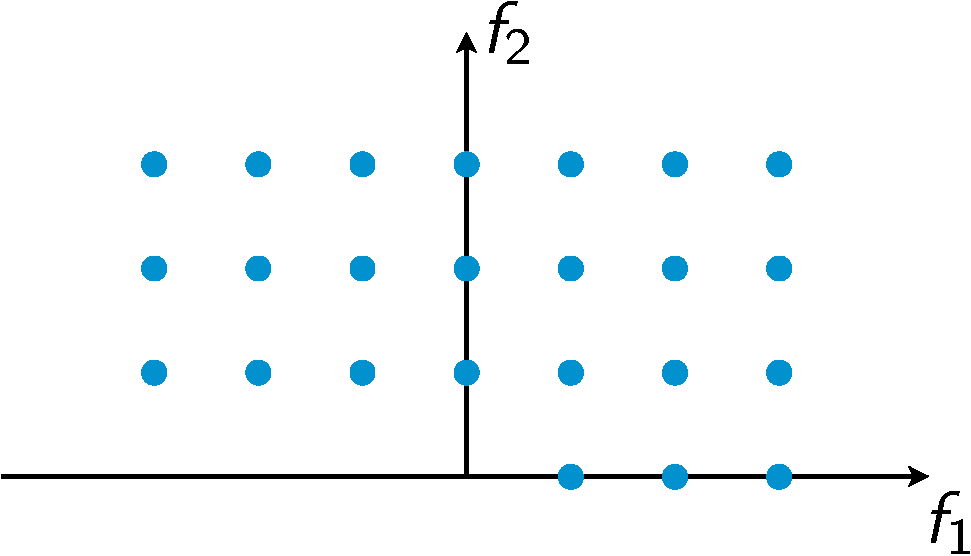
\includegraphics[width=.25\textwidth]{truncation_square.pdf}}
  \subfigure[diamond grid]{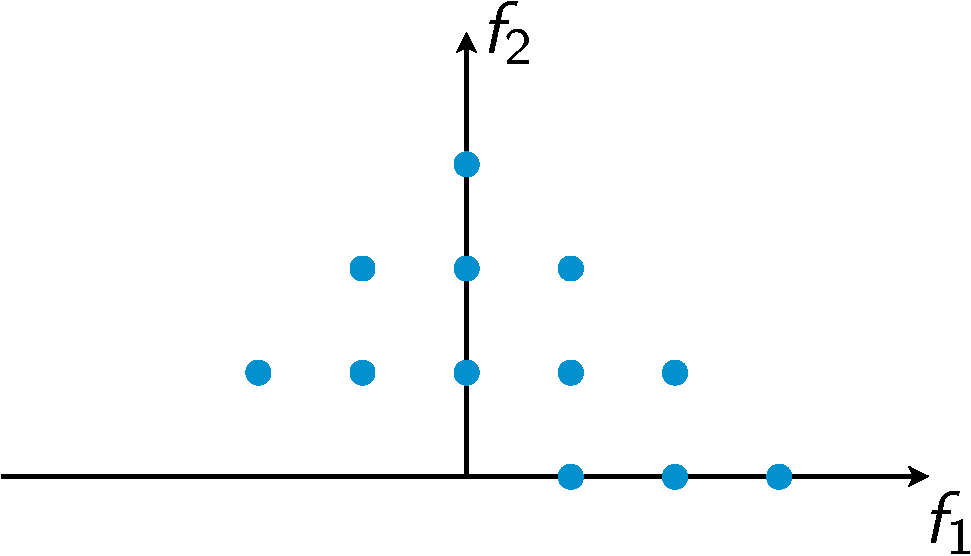
\includegraphics[width=.25\textwidth]{truncation_diamond.pdf}}
  \subfigure[cross grid]{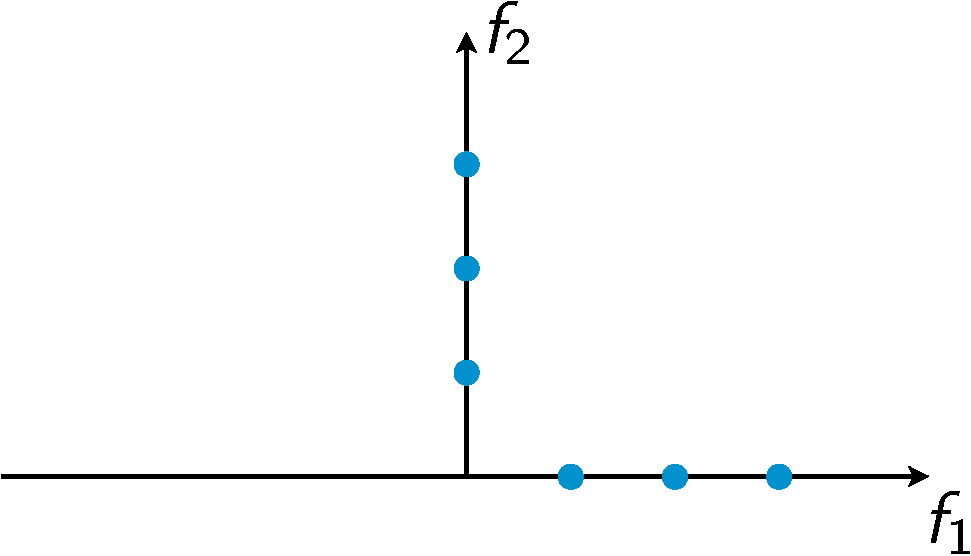
\includegraphics[width=.25\textwidth]{truncation_cross.pdf}}
  \caption{Truncation grids for reducing the set of frequencies of multi-frequential
  harmonic balance computations.}
  \label{fig:dream_hb_truncation}
\end{figure}
In the turbomachinery literature, \citet{Gopinath2007} follows the
diamond grid pattern while \citet{Ekici2007} seems to choose a
square grid pattern. In his PhD thesis, \citet{ThesisGuedeney}
first choose the frequencies by knowing which one emerge based on
a reference classical time-marching computation. Of course,
this approach can only be done \emph{a posteriori} which limits
the predictability of the method. He
also made computations with a "cross grid" truncation 
(shown in Fig.~\ref{fig:dream_hb_truncation}), this new type 
of truncation scheme only considers the harmonics of the
base frequencies. \citet{ThesisGuedeney} showed that this
truncation pattern gives
similar if not better results that the
"diamond grid" truncation pattern.  This "cross grid"
truncation pattern will be used in the current PhD work
when using the multi-frequential approach.

\paragraph{Aeroelastic simulations}

\citet{Thomas2002a} used the method to
determine the Limit-Cycle Oscillation (LCO) solution
of a transonic airfoil configuration using the
Euler equations and \citet{Thomas2004b} extended
it to the viscous Navier-Stokes equations.
For external-flow aeroelasticity, the HB approach has 
been thoroughly 
validated by \citet{Gopinath2005, JSicot2008, Woodgate2009, JDufour2009}, 
mostly for the AGARD test cases of \citet{Davis1982}. 
\citet{JDufour2009} highlight the benefits of using a 
non-linear approach for oscillating-flap simulations
compared to linearized approaches. A one-harmonic HB simulation
gives results comparable to an expensive time-marching simulation.
\citet{Huang2013} applied the mono-frequential
HB method to the flutter prediction of the 
$11\textsuperscript{th}$ 
standard configuration for aeroelasticity~\cite{Fransson1999}.
They show that with only one harmonic, the local
harmonic response of the fluid is superimposed
with the results of a time-marching simulation.
The same study has been performed in this PhD work
as detailed in Chap.~\ref{cha:stcf11}
and the same conclusions are drawn. These results have been
published as \citet{JSicot2012}.
In the context of the current thesis,
\citet{JSicot2013} applied the multi-frequential method to the
aeroelasticity of a contra-rotating fan, proving
the maturity of the method.


\paragraph{Transient problems}
\citet{Mavriplis2012} extended the method to 
an hybrid polynomial-harmonic balance approaches. 
It allows to use the method for maneuver simulations, 
where a part of the simulation exhibits a physical transient.
The method is also extended to overlapping mesh grids.

% \paragraph{Time sampling in the case of multi-frequential formulation}
% \citet{Gopinath2007} and \citet{Ekici2007}
% applied the multi-frequential method to
% a two-dimensional multistage compressor called
% configuration D. \citet{Ekici2007} use
% $3N+1$ evenly spaced 
% time instances to improve the condition number
% of the source term while \citet{Gopinath2007}
% stays with $2N+1$ evenly spaced time instances.
% \citet{Ekici2008a} applied the multi-frequential method
% to the effect of wake passing on the vibration of
% a turbine blade and uses $2N+1$ evenly spaced
% time instances are considered.
% \citet{JGuedeney2013} introduce non-uniform 
% time instances to minimize the condition number of multi-frequential
% computations. 
% The effect of the condition number on the stability
% of the computations is assessed along with algorithms
% to optimize the choice of the time instances.
% This allows to drastically reduce the condition number for
% any combination of frequencies, 
% while keeping only $2N+1$ samples.
% The method is then applied
% to a $1.5$ stage subsonic compressor.
% Note that a part of this work has been done in this
% thesis and will be detailed latter on.

\paragraph{Gradient-based method to determine the frequency}
With the same approach as \citet{McMullen2002}, \citet{Gopinath2006}
developed a gradient-based method to estimate the frequency of a 
vortex shedding behind a cylinder and a NACA0012 airfoil 
at high angle of attack using the harmonic balance approach.
The results are superimposed with a classical time-marching approach ones.

\paragraph{Optimum shape design}
\citet{Thomas2005b} used an automatic 
differentiation compiler to derive an adjoint code
from their harmonic balance code. This adjoint code is then
evaluated on the NLR~7301 supercritical airfoil section.
The computation of the sensibilities is finally
classically compared to a finite-difference and shows
to be in good agreement with these, validating
the given approach.

\paragraph{Adaptive method}
\citet{Maple2004} presented an adaptive harmonic
balance approach. The number of harmonics is increased
if the energy of the last harmonic divided by the cumulative
sum of the energy of each harmonic is larger than a 
given threshold. During the first iterations, only
a low number of harmonic is kept. Then, when the flow
is almost converged, the adaptive harmonic balance
approach is used. This ensures that higher order harmonics
are not injected at the first iterations, when the
flow is not physical. A $86\%$ reduction in time (and
in memory footprint) is seen compared to a resolved (converged in
terms of harmonics $N$) harmonic
balance computation. This has to be compared to
the $2$ factor speed-up observed by \citet{Mosahebi2013}
with an adaptive NLFD approach.

\subsection{Cost of the method}
\label{sec:sm_hb_cost}
As mentioned before, the cost of the method is linked to
the number of simulated time instances.
In fact, each new time instance corresponds to an additional steady computation.
Thus, if \mbox{$2N+1$} time instances are considered and if $\mathdollar_{\text{RANS}}$ 
denotes the CPU and memory cost of
one steady computation, the cost of the HB method can be 
approximated by:
\begin{equation}
	\mathdollar_{\text{HB}} = (2N+1) \times \mathdollar_{\text{RANS}}.
\end{equation}
Note that \citet{Ekici2007,Ekici2008a} use $3N+1$
time instances or more to solve the bad conditioning of the
source term when using the multi-frequential formulation. 
'This will be detailed latter on this thesis in 
Chapter~\ref{cha:limitations_condition_number} and an innovative solution
will be proposed. In that
case, the cost is bigger and scales with the chosen number
of time instances.


\section{Convergence of the spectral operator}
\label{sec:spectral_accuracy}
%!TEX root = ../../../adrien_gomar_phd.tex

In Chapter~\ref{cha:limitations_convergence}, we will
see that using Fourier-based time methods to compute
CROR configurations can show a very slow convergence. Here,
we recall the mathematical framework to understand the convergence
of Fourier-based time methods. A thorough study applied on CROR
simulations is provided in Chap.~\ref{cha:limitations_convergence}.

The convergence of the spectral operator depends on
the regularity of the approximated function. Consider a function
$u(t)$ that is continuous, periodic and bounded in $[0,T]$
and let $P_N \left(u(t)\right)$ denote its truncated Fourier series:
\begin{equation}
    P_N \left(u(t)\right) = \sum_{k=-N}^{N} \widehat{u}_k e^{i k\omega t}.
\end{equation}
The $\mathcal{L}2$-norm of the error writes:
\begin{equation}
   \| u \|_2 = \left(\int_0^T |u(t) - P_N \left(u(t)\right)|^2 \diff t \right)^{1/2}.
\end{equation}
If $u(t)$ is m-times continuously differentiable in $[0,T]$ ($m \geq 1$) 
and its $j$-th derivative is periodic on $[0,T]$ for all $j \leq m - 2$
then, it exists  $k_0 \in [1, N]$ such that for $k > k_0$:
\begin{equation}
    \widehat{u}_k = \mathcal{O} (k^{-m}),
\end{equation}
where $\widehat{u}_k$ is the k-th Fourier coefficient of $u(t)$.
This equation means that, the more regular the function is,
the faster the convergence rate of the Fourier
coefficients.
The property of the error to decay exponentially as soon as 
the function is approximated by a number of harmonics greater than $k_0$ 
is called spectral accuracy~\cite{Canuto2006}. Note that
$k_0$ is not known but is rather essential for the analysis.
For $k$ below $k_0$, approximating the function $u(t)$ with its Fourier
series yields unacceptably high errors.

% ===================================
% = Periodic flows in turbomachines =
% ===================================
\section{Periodic flows in turbomachines}
\label{sec:sm_hudson}
%!TEX root = ../../../adrien_gomar_phd.tex

In this thesis, the final application is contra-rotating open rotor
configurations. To bound Fourier-based time methods for such
applications, we propose a classification of the
unsteady phenomena that can be computed using such approaches.

Inspired by \citet{Hodson1998},
a diagram presenting the unsteadinesses seen in 
a CROR is shown in Figure~\ref{fig:hudson}. A distinction
is made between unsteadinesses whose frequencies are
known or not.
\begin{figure}[htp]
  \centering
  \includegraphics*[scale=0.8]{hudson.pdf}
  \caption{Main unsteady phenomenon seen by contra-rotating
  open rotors. Bold blue text highlights applications that can
  be treated with the harmonic balance implementation available for the
  current thesis and underlined red text shows additional applications
  made possible by extensions available in the literature.}
  \label{fig:hudson}
\end{figure}
From the bibliography presented previously, almost all
unsteady flows can be computed using Fourier-based time methods.
The current implementation of the HB method available for
this thesis is able to compute all the unsteadinesses highlighted
by a bold text. In the literature, the presented work of 
\citet{Mavriplis2012} allows to compute transient unsteady flow
resulting from a change of operating point and/or a maneuver and
the work of \citet{McMullen2002} and \citet{Gopinath2006} allows
to capture periodic flows whose frequency is unknown. These two
kinds of unsteadiness are added
to the current panel of applications that can
be treated by Fourier-based time methods. Let us note
that the gradient algorithm presented by \citet{McMullen2002}
and \citet{Gopinath2006} is only able to converge when a 
good approximate of the solution is given, meaning
that this strategy fails when one has no estimate
of the value of the frequency for the considered phenomenon.
It can also be inferred that using such an optimization algorithm
coupled with a Fourier-based time method
might require more computational time than a classical time-marching scheme,
which limits its applicability to academical configurations.



\chconclu{Four Fourier-based methods have been presented in this chapter.
The main mathematical developments have been demonstrated and 
the hypothesis/weakness of each method has been highlighted.
In particular, the presented harmonic balance method can
treat both mono- and multi-frequential applications. One
unsteady equation is transformed into a subset of $2N+1$
steady-state equations coupled by a source term which
is analytical in the mono-frequential formulation and
of matrix form in the multi-frequential framework.
The large literature available on these methods shows that
they are ready for industrial, numerically demanding
unsteady applications. Moreover, the method is able to
efficiently compute aeroelastic phenomenon on 
contra-rotating configurations motivating its
use in the present thesis.}


\part{Advantages and limitations of Fourier-based methods}
\label{part2}
%!TEX root = ../../../adrien_gomar_phd.tex
\chapter{Validation of the harmonic balance approach}
\label{cha:validation_hb}

\chabstract{In this chapter the mono- and
multi-frequential harmonic balance approaches
are validated. In this aim, two toy problems are used.
Firstly, the HB method is applied to the linear advection equation 
supplemented with unsteady boundary conditions 
of different frequency content. Mono- and multi-frequential
unsteady signals are injected and compared to the
analytical results. The property of spectral accuracy is retrieve.
Moreover, the ability of the multi-frequential
approach to capture signal composed of segregated frequencies
is underlined. Based on these results, the aeroelasticity
of contra-rotating open rotors is put into perspectives.
Secondly, the multi-frequential approach is assessed on
a channel flow problem solved using the \emph{elsA}~\cite{Cambier2013}
CFD code within the Navier--Stokes equations framework. The results
are shown to be superimposed with a classical time-marching solution.}

\newpage

\section{Within a linear framework}
\label{sec:linear}
%!TEX root = ../../../adrien_gomar_phd.tex

\subsection{Presentation of the test case}
\label{sec:presentation_advection}

To validate the harmonic balance approach within a 
linear framework, the resolution of the
advection equation is considered. It is defined as
\begin{equation}
  \label{eq:convection}
  \frac{\partial u}{\partial t} + c \frac{\partial u}{\partial x} = 0,
\end{equation}
with the constant advection speed $c$ assumed as positive. 
The equation is solved in the domain $x \in [0, L_x]$. 
Periodic perturbations of different shapes are imposed at the left boundary
\begin{equation}
   u(0, t) = u_l (t),
\end{equation}
where $u_l$ is a periodic function of period $T=L_x/c$.
These perturbations are advected across the computational 
domain and leave from the right boundary. After a transient of time length $T_{trans}=L_x/c$, 
the solution at any point $x$ in the space domain achieves a periodic state. 
The exact solution for this periodic state is a periodic function of the form
\begin{equation}
    u_{ex}(x,t)=u_l(x/c+t).
\end{equation}
For simplicity, $L_x$ and $c$ are taken as unity.

\subsection{Numerical setup}

The space derivative is discretized by means of a centered 
fourth-order finite-difference scheme on a uniform Cartesian mesh
\begin{equation}
    \frac{\partial u}{\partial x} (x = x^i, \replaced{\tau=\tau_q}{t=t_q}) =
    \frac{-u^{i+2}_{q} + 8 u^{i+1}_{q} - 8 u^{i-1}_{q} + u^{i-2}_{q}}{12\Delta x}
    + \mathcal{O} (\Delta x^4),
    \label{eq:convection_center4}
\end{equation}
A very fine space step is used ($\Delta x=5\e{-4}$) in order to rule 
out spatial approximation errors. This corresponds to $2,000$ grid points
in the domain. 
The solution at the last mesh 
point on the right of the domain is extrapolated 
from the inside. To this aim, a standard second-order 
and a first-order upwind discretization schemes
are used to approximate the space derivative at 
the last two mesh points on the right, respectively
\begin{equation}
    \begin{split}
        &\frac{\partial u}{\partial x} (x = x^{m-1}, \replaced{\tau=\tau_q}{t=t_q}) =
            \frac{3 u^{m-1}_{q} - 4 u^{m-2}_{q} + u^{m-3}_{q}}{2\Delta x} + \mathcal{O} (\Delta x^2), \\
        &\frac{\partial u}{\partial x} (x = x^m, \replaced{\tau=\tau_q}{t=t_q}) = 
            \frac{u^{m}_{q} - u^{m-1}_{q}}{\Delta x} + \mathcal{O} (\Delta x),
    \end{split}
\label{eq:upwind_scheme}
\end{equation}
where $m$ is the total number of grid points.

Time-discretization is achieved 
through the HB method (described in Sec.~\ref{sec:sm_hb})
with a standard four-step Runge-Kutta method~\cite{Jameson1981}
used to pseudo-time 
march the HB equations to the steady-state.
The $k\textsuperscript{th}$ step is evaluated by
\begin{equation}
    u_k = u_q - \alpha_k \replaced{\Delta \tau}{\Delta t} \left [ 
          c \frac{\partial u_{k-1}}{\partial x} 
          (\replaced{\tau=\tau_q}{t=t_q} + \alpha_{k-1} \replaced{\Delta \tau}{\Delta t})
          + D_t(u_k)
          \right],
    \label{eq:convection_rk4}
\end{equation}
where $\alpha_0 = 0$, $\alpha_1 = 1/4$, 
$\alpha_2 = 1/3$, $\alpha_3 = 1/2$, $\alpha_4 = 1$. 
The HB source term $D_t(u_k)$ is computed 
using Eq.~\eqref{eq:sm_multi_spectral_operator}.

\replaced{The CFL number in pseudo-time is set to 1 
to ensure the stability of the explicit time-marching scheme
which sets the time step.
For stability reasons, this time step
is modified~\cite{Weide2005} to take into account
the additional source term
\begin{equation}
  \label{eq:stabdeltat}
  \Delta\tau = \text{CFL} \frac{\Delta x}{c + \omega N \Delta x}.
\end{equation}
The extra term $\omega N \Delta x$ is added 
to the advection velocity $c$ to
restrict the time step.  Equation~\eqref{eq:stabdeltat} implies that a
high frequency and/or a high number of harmonics~$N$ can considerably
restrict the time step, especially for explicit Runge Kutta time
integration scheme, as mentioned in~\cite{Hall2002}. Moreover, for 
the multi-frequential
computations, the extra term $\omega N \Delta x$ is
replaced by $\omega_N \Delta x$, where $\omega_N$ denotes
the largest angular frequency.}{
The CFL number in pseudo-time is set to 1 
to ensure stability of the explicit time-marching scheme.}

\subsection{Validation of the mono-frequential approach}
\label{sec:sum_sine}

A perturbation 
in the form of a finite sum of sine functions, similar to the one used
in Sec.~\ref{sec:hb_operator},
is applied at the left boundary
\begin{equation}
    u_l(t) = \cos(\omega t) + \sin(2 \omega t) +
    \cos(3 \omega t) + \sin(4 \omega t) + \cos(5 \omega t).
    \label{eq:sum_injected_fct}
\end{equation}
Harmonic balance computations are run with 1 to 10~harmonics.
For each computation, we show spatial distributions of the solution
at three time instants, namely $t=0$, $t=T/3$ and $t=2T/3$.
Since these instants are not necessarily used in the HB discretization,
a temporal interpolation is performed.
To do so, the frequency content of the HB solution is used
together with an inverse Fourier transform on the time-vector
$[0, T/3, 2T/3]$.
Figure~\ref{fig:inj_sine_results} depicts the results of HB computations
using 1 to 5~harmonics. The analytical solution is also reported for comparison.
\begin{figure}[htp]
  \centering
  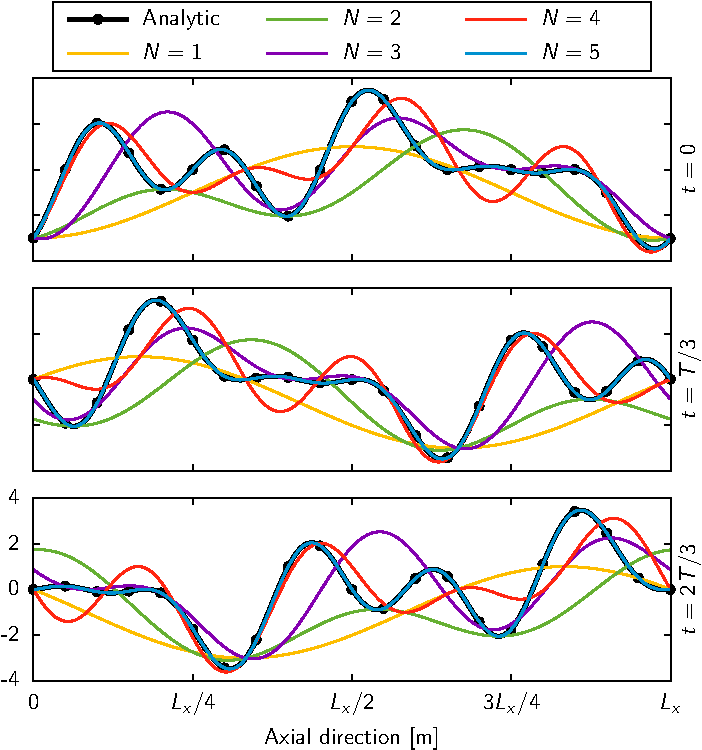
\includegraphics[width=.5\textwidth]{convection_sin.pdf}
  \caption{Linear advection of a sum of sine functions: 
  numerical solutions at different time instants for different numbers of harmonics.}
  \label{fig:inj_sine_results}
\end{figure}


The accuracy of the solution 
improves with the number of harmonics,
until it reaches the frequency content
of the injected signal, \emph{i.e.} 5~harmonics.
For higher sampling levels, the results of HB computations are
superimposed with the analytical solution, validating the current approach.

The $\mathcal{L}_2$-norm of the error 
in time is computed over all the time instants
at each grid point over the domain.
Then, the average in space is computed.
The error is shown as a function of the number of harmonics
in Figure~\ref{fig:conv_sum_sine}. Two results are displayed:
one for the reference mesh (2,000 grid points) and one for
a refined mesh (4,000 grid points).
\begin{figure}[htp]
  \centering
  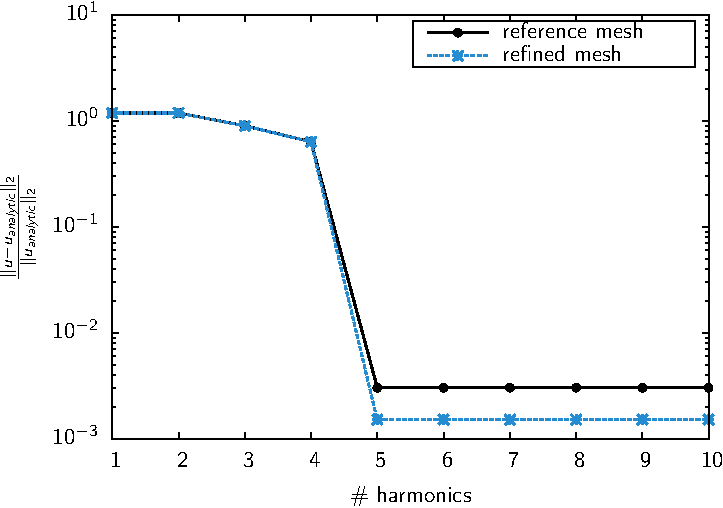
\includegraphics[width=.5\textwidth]{convection_sin_error.pdf}
  \caption{Linear advection of a sum of sine functions: convergence of the HB method error.}
  \label{fig:conv_sum_sine}
\end{figure}
The convergence of the HB computations is slow  for
$N \leq 4$. However, when the number of harmonics composing
the injected function is reached ($N=5$), the error is minimum and computing
more harmonics does not change the error. As introduced in 
Sec.~\ref{sec:spectral_accuracy},
the convergence rate 
of Fourier-based time methods is inherently linked to the spectrum of the
temporal phenomenon that one wants to capture. This property is still
seen when solving the linear advection equation.
Here a finite discrete spectrum composed of only five harmonics
is imposed.
The value of the plateau obtained 
after $N=5$ is representative of the error introduced by the different
discretizations. In fact, refining the mesh changes this value
without modifying the error levels of the lower harmonics points
as indicated by Figure~\ref{fig:conv_sum_sine}.

The temporal discrete Fourier transform
of the computational results is compared to the
analytical results in Figure~\ref{fig:dft_sin}.
\begin{figure}[htp]
  \centering
  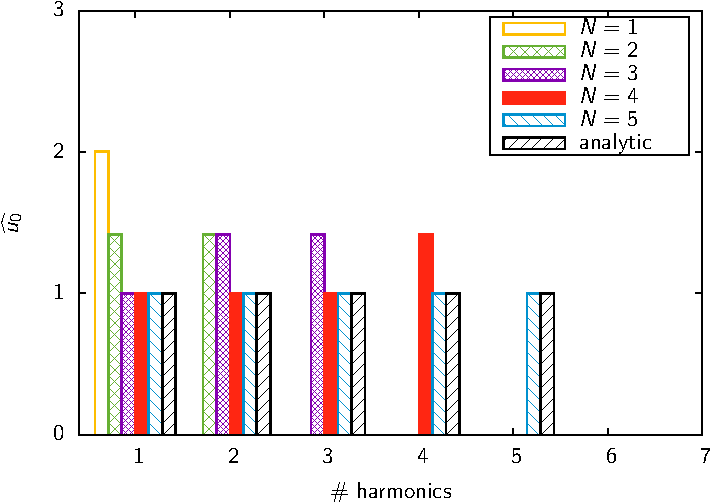
\includegraphics[width=.5\textwidth]{convection_sin_dft.pdf}
  \caption{Linear advection of a sum of sine functions: 
  discrete Fourier transform.}
  \label{fig:dft_sin}
\end{figure}
When the number of harmonics grows in the spectral computations,
the Fourier transform gets closer to the analytical solution.
When the whole frequency content of the injected 
function is contained in the HB solution, 
the numerical results are superimposed with the analytical ones.
For intermediate sampling frequencies, as for 
instance the three-harmonics HB computation, 
the resolved harmonics have higher amplitudes 
than the exact one, since they compensate for harmonics that are not resolved.

When the number of harmonics composing the spectrum of the
computed signal is reached, the computational results are superposed
with the analytical ones, namely we obtain spectral accuracy.
This is the main advantage of Fourier-based time methods: when the
signal has a narrow spectrum, as it is the case for the sum
of sine function used here, the
convergence can be very fast compared to a classical time-marching scheme
as only a few number of time instants is necessary to retrieve the
unsteadiness.


\subsection{Validation of the multi-frequential approach}

In Section~\ref{sec:sm_hb_multi}, the multi-frequential harmonic
balance approach has been presented. In this method,
the frequencies can be chosen arbitrarily. This becomes particularly
interesting when dealing with signal/flow field composed of segregated
frequencies. To emphasize that, let us consider the linear advection problem
with a perturbation 
in the form of a sum of two sine functions,
applied at the left boundary
\begin{equation}
    u_l(t) = \sin(\omega t) + \sin(22 \omega t).
    \label{eq:multifreq_inj_func}
\end{equation}

\subsubsection{Using a mono-frequential approach}

Obviously, computing the advection of such a perturbation using
a classical time-marching scheme would require to discretize the
smaller period. The largest frequency
(here $f_2 = 22$~Hz) acts as a bottleneck as the time-step will be chosen
according to this frequency. The cost scales thus with the ratio of $f_2 / f_1$.

This holds true when computing the solution using the mono-frequential
harmonic balance approach. In fact, the frequencies can not be chosen arbitrarily.
Therefore, to compute such a configuration, a $N=22$ harmonic computation
will be needed to be spectral accurate. To emphasize that, mono-frequential
HB computations are run with 1 to 25~harmonics.
As made previously, 
for 6 chosen computations of the~25 computations, 
we show spatial distributions of the solution
at three time instants, namely, $t=0$, $t=T/3$ and $t=2T/3$.
It is shown in Figure~\ref{fig:inj_multifreq_tsm}.
\begin{figure}[htp]
  \centering
  \subfigure[$N=1$]{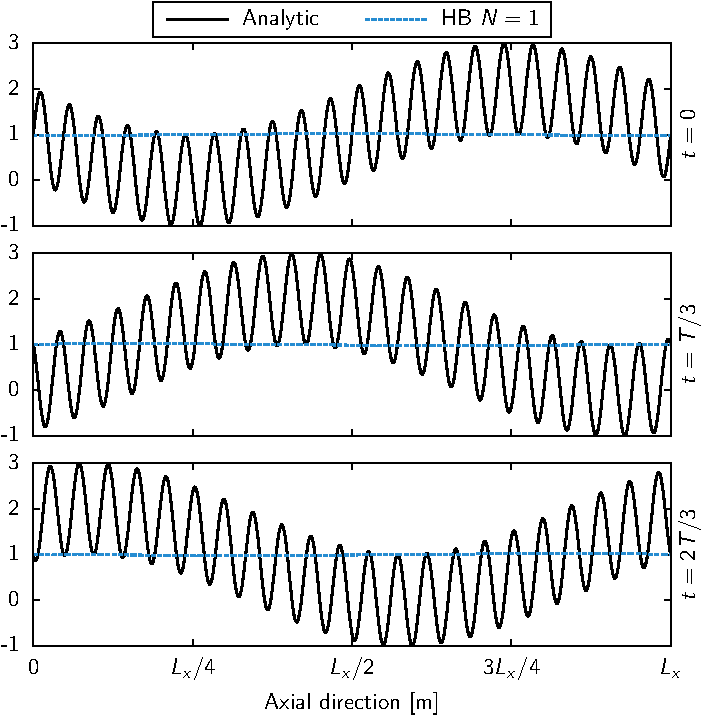
\includegraphics[width=.35\textwidth]{convection_multifreq_tsm_N1.pdf}}
  \subfigure[$N=5$]{
    \label{fig:convection_multifreq_tsm_N5}
    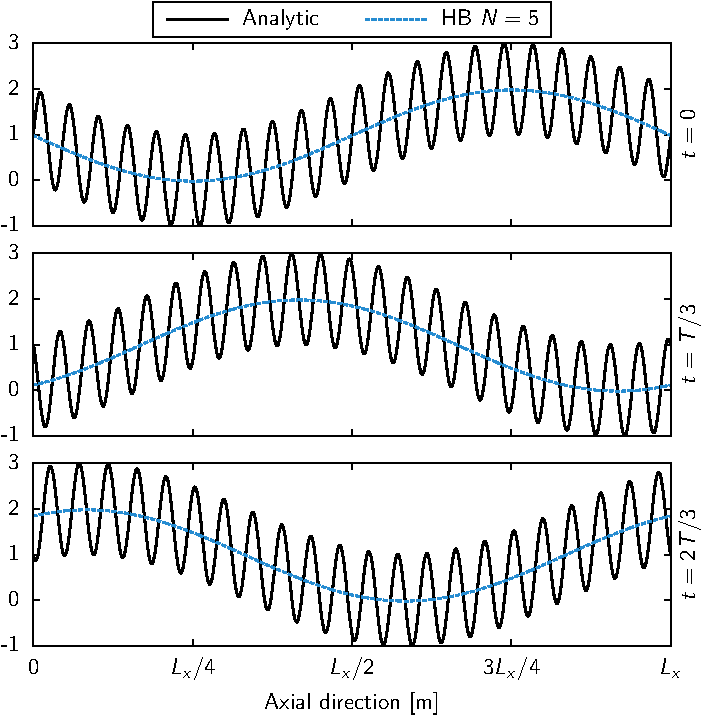
\includegraphics[width=.35\textwidth]{convection_multifreq_tsm_N5.pdf}}
  \subfigure[$N=11$]{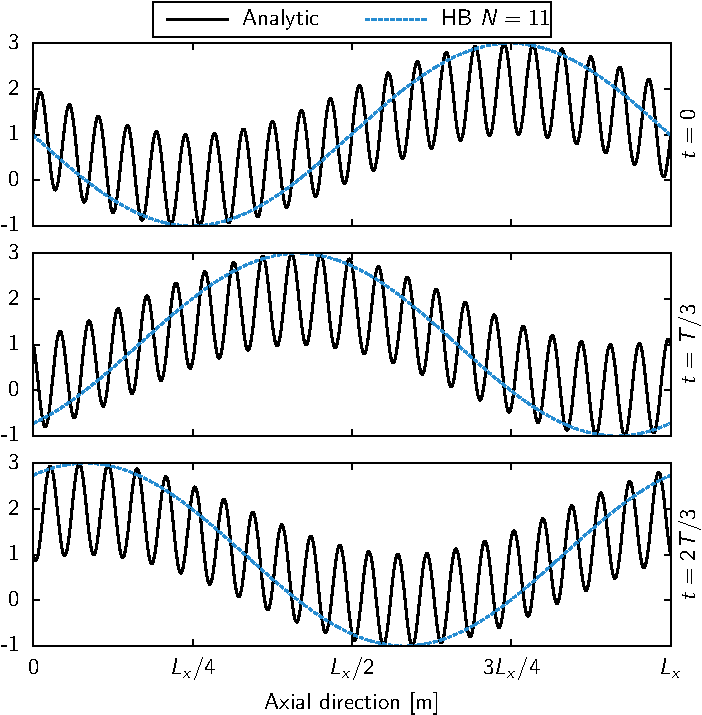
\includegraphics[width=.35\textwidth]{convection_multifreq_tsm_N11.pdf}}
  \subfigure[$N=16$]{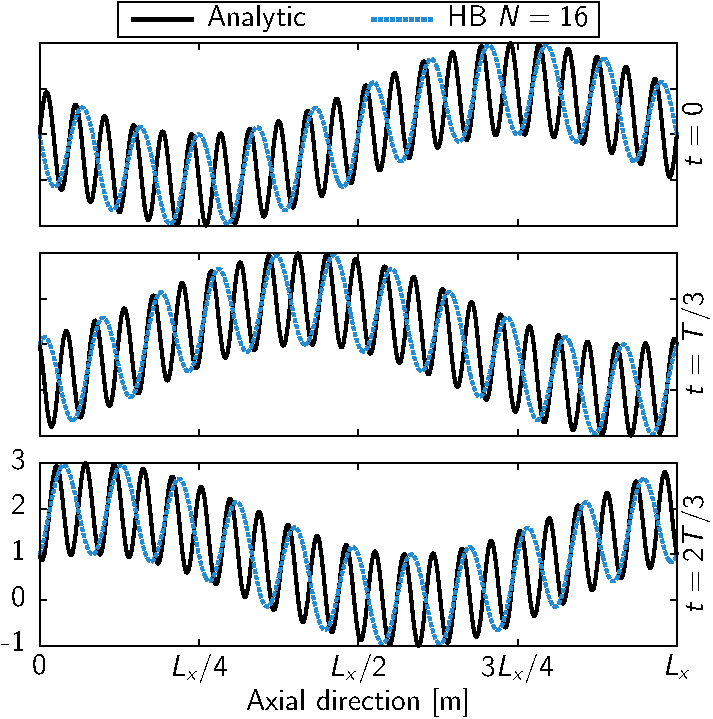
\includegraphics[width=.35\textwidth]{convection_multifreq_tsm_N16.pdf}}
  \subfigure[$N=22$]{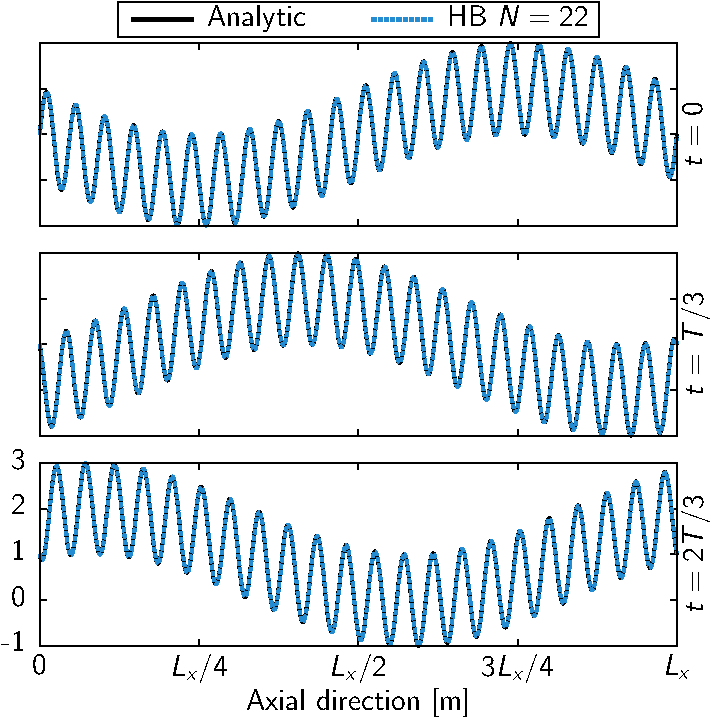
\includegraphics[width=.35\textwidth]{convection_multifreq_tsm_N22.pdf}}
  \subfigure[$N=23$]{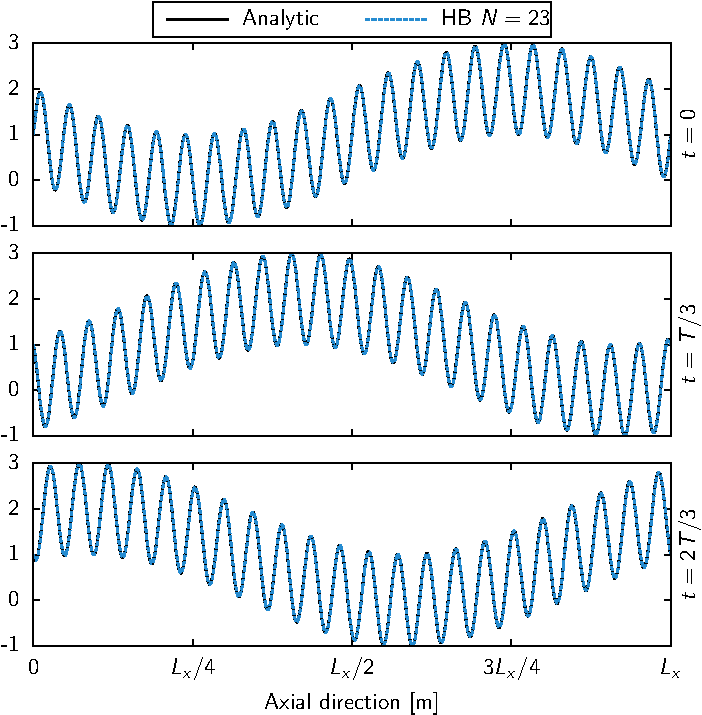
\includegraphics[width=.35\textwidth]{convection_multifreq_tsm_N23.pdf}}
  \caption{Linear advection of a sum of two segregated sine functions: 
  numerical solutions at different time instants for different numbers of harmonics.}
  \label{fig:inj_multifreq_tsm}
\end{figure}
Again, the accuracy in capturing the injected function
improves with the number of harmonics,
until it reaches the frequency content
of the injected signal, \emph{i.e.} 22~harmonics.
After that, the results of the HB computations are
superimposed with the analytical solution. 
The problem, with such a segregation of frequencies, is that 
the mono-frequential version suffers from the same
problems as a classical time-marching scheme in terms of 
computational cost.

To quantitatively analyze the results,
the discrete $\mathcal{L}_2$-norm of the error 
is shown in Figure~\ref{fig:conv_multifreq_tsm} for the
mono-frequential HB computations ranging from 1 to~25
harmonics.
\begin{figure}[htp]
  \centering
  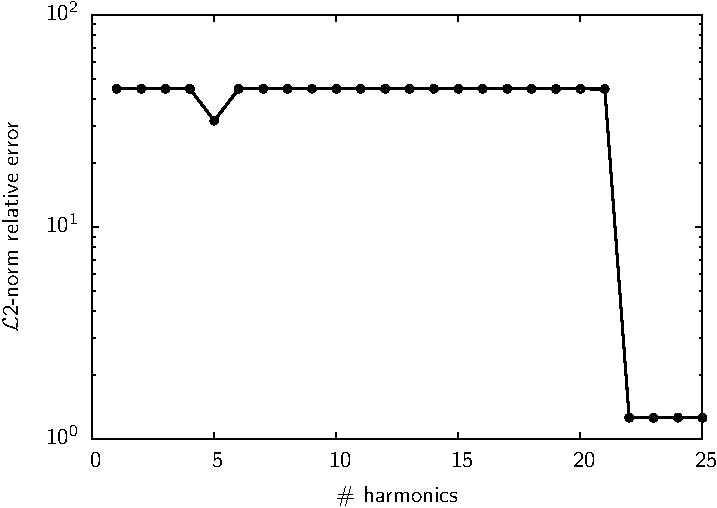
\includegraphics[width=.5\textwidth]{convection_multifreq_error.pdf}
  \caption{Linear advection of a sum of two segregated sine functions: convergence of the mono-frequential HB method error.}
  \label{fig:conv_multifreq_tsm}
\end{figure}
When the number of harmonics
used to compute the solution is higher than the content of the spectrum,
the error decreases drastically. The spectral accuracy is retrieved
but only starting at $N=22$.
In fact, similar as in Sec.~\ref{sec:sum_sine},
the injected function is indefinitely differential and periodic
yielding an infinite convergence slope. We can observe a slight local convergence
for the $N=5$ harmonics HB computation. This is due to the fortunate 
capture of the low-frequency pattern of the injected function
as shown in Figure~\ref{fig:convection_multifreq_tsm_N5}.

\subsubsection{Using a multi-frequential approach}

One of the advantage of the multi-frequential HB method, 
introduced in Sec.~\ref{sec:sm_hb_multi}
and used in this work, is that it can take arbitrary frequencies into account.
In the case of an injected signal with a large frequency segregation, the
benefit might be tremendous. Let us consider again the signal defined in 
Eq.~\eqref{eq:multifreq_inj_func} and compute one HB simulation using 
$f_1=1$~Hz and $f_2=22$~Hz as input frequencies. This gives a computation
of two coupled calculation
that is nine times faster than the $N=22$ converged mono-frequential
HB computation. \added{In fact, the cost of a $N=22$ computation scales with
$2 \times 22 + 1=45$ (see Sec.~\ref{sec:sm_hb_cost}), 
while a $N=2$ computation scales with $2 \times 2 + 1=5$
which explains the nine factor.}

Again
we show spatial distributions of the solution
at three time instants, namely $t=0$, $t=T/3$ and $t=2T/3$
in Figure~\ref{fig:inj_multifreq_hb}.
\begin{figure}[htp]
  \centering
  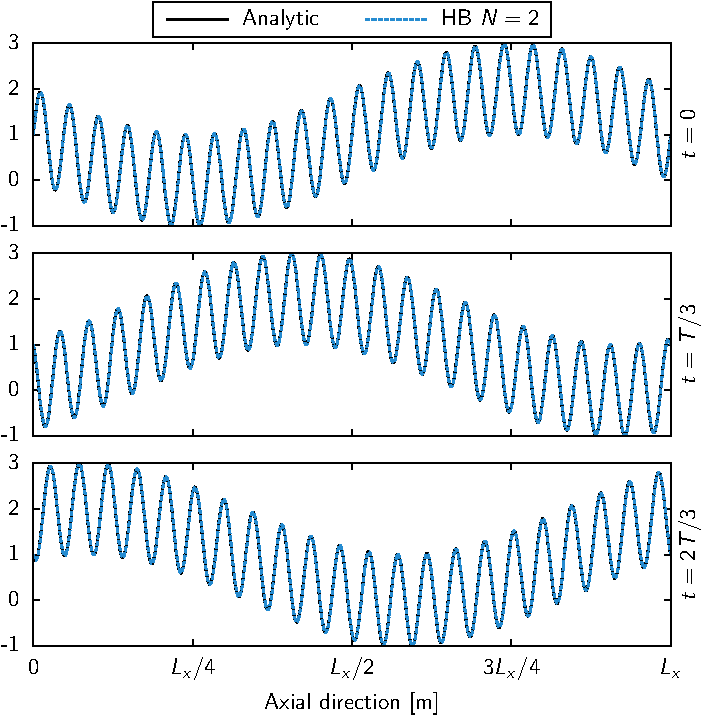
\includegraphics[width=.5\textwidth]{convection_multifreq_hbt_N2.pdf}
  \caption{Linear advection of a sum of two segregated sine functions: 
  numerical solutions at different time instants for different numbers of harmonics using the
  multi-frequential harmonic balance method.}
  \label{fig:inj_multifreq_hb}
\end{figure}
With only two input frequencies, the multi-frequential
HB solution is superimposed with the analytical solution.
Moreover, the $\mathcal{L}2$-norm of the error is 
exactly the same as the one of the $N=22$ mono-frequential
approach.

This validates the multi-frequential approach 
used along with segregated frequencies which is 
the case of contra-rotating open rotor aeroelasticity.


\section{Within a non-linear framework}
\label{sec:non_linear}
%!TEX root = ../../../adrien_gomar_phd.tex
\subsection{Presentation of the case}
\label{sec:channel_flow_problem}

The second toy problem considered represents a 2D channel 
with a constant left injection at 
a transonic Mach number ($M=0.7$)
supplemented with a time-varying unsteady back pressure.
As the pressure is oscillating at the outlet, the imposed unsteady pressure
fluctuations travel within the flow at the velocity 
$u + c$ and $u - c$, where $u$ denotes 
the local flow velocity and $c$ the speed of sound.
Since the pressure waves are generated at the outlet, only
the $u-c$ waves are seen, resulting in pressure waves propagating
upstream of the channel. The axial length of the channel is $L_x = 100$~m
and $L_y = 1$~m in the transverse direction.
Figure~\ref{fig:canal_principle} shows a sketch
of the considered channel flow problem.
\begin{figure}[htp]
  \centering
  \includegraphics*[width=0.65\textwidth]{channel_sketch.pdf}
  \caption{Sketch of the channel flow problem.}
  \label{fig:canal_principle}
\end{figure}

\citet{Merkle1987} give an analytical solution
for incompressible flows with small pressure fluctuations, assuming
thus a linear unsteady flow.
However, this toy problem is set up to highlight the properties
of the harmonic balance in a non-linear framework which is not
the hypothesis of \citet{Merkle1987}. Nevertheless, to give confidence
in our forthcoming results for this toy problem,
this last will be validated below against a classical time-marching scheme
in Sec.~\ref{sec:channel_multifreq}.

\subsection{Numerical setup}

% mesh presentation
The mesh consists of 997~points along the axial direction and 9~in the
transverse one, which corresponds to equal spacings in both
directions. 

% boundary conditions
The boundary conditions are: (i)~a constant injection condition for the inlet
where the total pressure $p_{i_0}$ and enthalpy $h_{i_0}$ are set,
(ii)~symmetric conditions for the upper and lower bounds as the flow
is assumed to be symmetric in the transverse direction, and (iii)~a
fluctuating static pressure imposed at the outlet:
\begin{equation}
  p_{s_1}(t) = \overline{p}_{s_1} \left[1 + a_1 \sin(2 \pi f_1 t) +
    a_2 \sin(2 \pi f_2 t) \right],
  \label{eq:outlet_canal}
\end{equation}
where $\overline{p}_{s_1}$ is the temporal average static pressure, $a_n$ the
amplitude of the $n$\textsuperscript{th} mode and $f_n$ its
frequency. Only two modes ($f_1$, $f_2$) are injected
but due to the non-linearity of the Navier--Stokes equations,
new frequency combinations rise.
The mean velocity of the flow is imposed through a
static pressure condition $\overline{p}_{s_1}$ at the outlet:
\begin{equation}
    \overline{p}_{s_1} = \frac{p_{i_0}}{\left(1 + 
    \frac{\gamma - 1}{2} M_{0}^2 \right) ^ {\frac{\gamma}{ \gamma - 1}}} ,
\end{equation}
the mean velocity is thus set by imposing the
inlet target mean Mach number value $M_{0}$.
We assume here that the flow is isentropic as no
geometrical object disturbes the flow field.

% solver
The \textit{elsA}~\cite{Cambier2013} CFD code developed by ONERA
is used to solve this toy problem. In fact, 
the aim of this toy problem is 
to use the same
solver as the one used in the application part of this
thesis so that the results shown here can be directly
transposed. 
This code solves the RANS equations using a cell-centered
approach on multi-blocks structured meshes.
Several time-integration schemes
are available, in particular the Dual Time-Stepping~\cite{Jameson1981} (DTS)
as well as the time-domain harmonic 
balance method implemented by \citet{JSicot2008} for the mono-frequential
formulation and extended by \citet{JGuedeney2013} to multi-frequential flows. 


% numerical schemes
The present configuration is turbulent as the Reynolds number based on the
inlet flow velocity and the axial length of the channel is about $R_e
\approx 2.0 \times 10^9$. To this aim, turbulence is modeled using the
one-equation model of \citet{Spalart1992}.
Roe's scheme~\cite{Roe1981} along with a third-order MUSCL extrapolation 
is used for the spatial discretization of
the convective fluxes. An implicit backward Euler scheme is used
to march the HB equations in pseudo-time.

\subsection{Validation of the multi-frequential approach}
\label{sec:channel_multifreq}

As no analytical solution is available for this case, we propose
now to validate the channel flow toy problem within a HB framework
in order to have confidence in the forthcoming results on this
toy problem.
To do so, two non-harmonically related
frequencies are chosen as input for the outlet boundary condition:
$f_1 = 3$~Hz and $f_2 = 17$~Hz.

The classical DTS time-marching scheme is taken for comparison.
Convergence in time discretization is obtained after 20~periods using
160~instants per almost-period. Since the frequencies are integers and
coprime, the period is $T=1$~s.  Iterative convergence for the
inner loop is considered achieved when the normalized residuals drop
by $10^{-2}$ within a maximum of 50~sub-iterations.

The results obtained with the DTS scheme are compared to the HB
results for pressure waves amplitudes of $a = a_1 = a_2 = 0.001$
(see Eq.~\eqref{eq:outlet_canal}).  The
transient of the DTS computation is shown in
Fig.~\ref{fig:canal2_transient}, illustrating the wave propagation
with a slight attenuation of the high-frequency waves.
\begin{figure}[htp]
  \centering
  \includegraphics*[width=.5\linewidth]{CANAL2_TRANSIENT_PPT.pdf}
  \caption{DTS computation: transient propagation of the pressure waves.}
  \label{fig:canal2_transient}
\end{figure}

Due to the non-linearity of the Navier--Stokes equation, the two frequencies
$f_1$ and $f_2$ give rise to linear combinations of them.
Therefore, the results are analyzed for frequencies $1<f< 40~\textrm{Hz}$ and the
dominant frequencies (the one that have the highest amplitudes) are
set for the HB computation.  To do so, pressure signals are probed
upstream, in the middle and downstream of the channel at
$x=[25~\textrm{m}, 50~\textrm{m}, 75~\textrm{m}]$ and $y=0.5$~m
respectively.  The spectrum of the aforementioned unsteady pressure
signals, obtained with a Fourier Transform is plotted in
Fig.~\ref{fig:canal2_dts_fft}.  The labeled frequencies are the
dominant ones, as for each probe, these have a high amplitude. Those
nine frequencies are thus selected as input frequencies for the HB computation.
\begin{figure}[htp]
  \centering
  \includegraphics*[width=.5\linewidth]{channel_dts_fft_plus_sketch.pdf}
  \caption{Spectrum of pressure signals.}
  \label{fig:canal2_dts_fft}
\end{figure}

The HB computation using the previously mentioned frequencies is
run and a discrete Fourier transform is computed at several axis positions
in the middle of the channel ($y=0.5$~m). 
This is the same post-processing as done previously to retrieve 
Fig.~\ref{fig:canal2_dts_fft}, but for all axial grid points.

Figure~\ref{fig:canal2_validation_hbt_gear_amp_vs_axis}
shows the results for the frequencies that have been set for the HB computation.
The overall agreement between the DTS and the HB is fair.  
Some local discrepancies can be
observed upstream for frequencies $f_2 + 3f_1$, $f_2 - f_1$ and $f_2 -
2f_1$. 
\begin{figure}[htp]
  \centering
  \includegraphics*[width=.5\linewidth]{CANAL2_VALIDATION_HBT_GEAR_PPT_AMP_VS_AXIS.pdf}
  \caption{Spatial evolution of the amplitude of the dominant
    frequencies in the channel flow configuration, for $f_1 = 3$~Hz and $f_2 = 17$~Hz.}
  \label{fig:canal2_validation_hbt_gear_amp_vs_axis}
\end{figure}
These are caused by aliasing
but they are minimal regarding the temporal evolution, as
shown in Fig.~\ref{fig:canal2_validation_hbt_gear_time_ev}, where the
time evolution of pressure signals is extracted at all probes.  The
difference between the HB and the DTS method is negligible proving
that the present toy problem can be used to analyze the properties of 
the HB method.
\begin{figure}[htp]
  \centering 
  \subfigure[probe
  1]{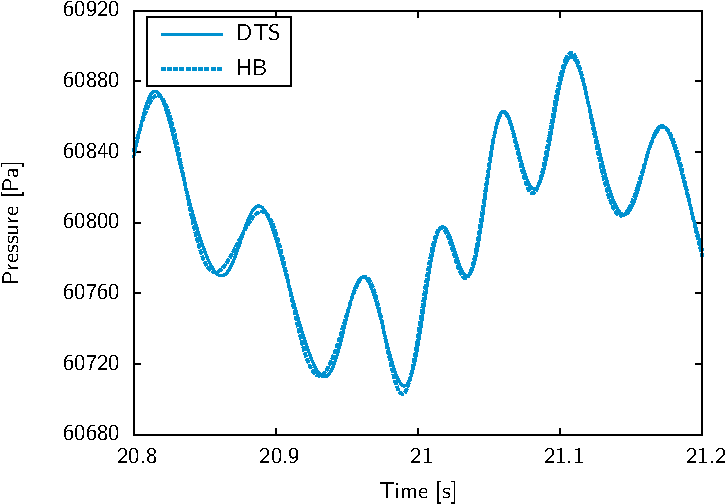
\includegraphics[width=.4\textwidth]{CANAL2_VALIDATION_HBT_GEAR_TIME_EV_PROBE_1_PPT.pdf}}
   \quad\subfigure[probe
   2]{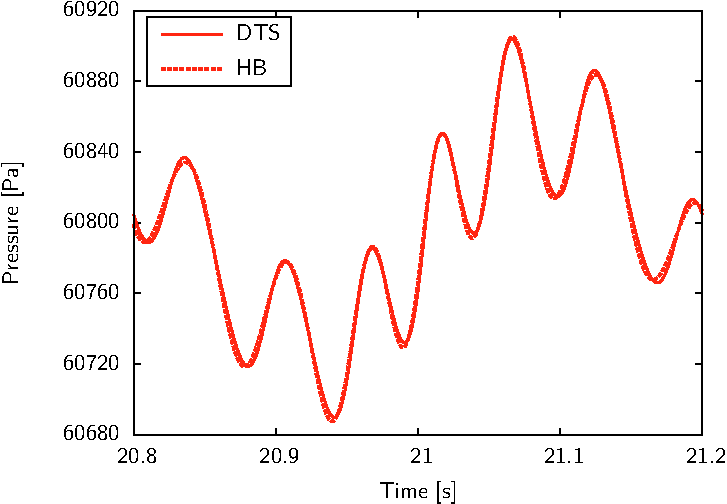
\includegraphics[width=.4\textwidth]{CANAL2_VALIDATION_HBT_GEAR_TIME_EV_PROBE_2_PPT.pdf}}
   \subfigure[probe
   3]{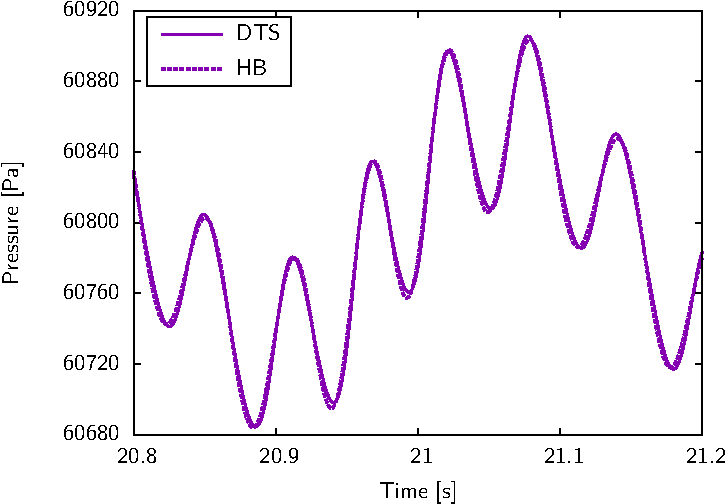
\includegraphics[width=.4\textwidth]{CANAL2_VALIDATION_HBT_GEAR_TIME_EV_PROBE_3_PPT.pdf}}
  \caption{Unsteady pressure signals at different axial positions.}
  \label{fig:canal2_validation_hbt_gear_time_ev}
\end{figure}


%!TEX root = ../../../adrien_gomar_phd.tex

\chapter{Conditioning of multi-frequential harmonic balance methods}
\label{cha:limitations_condition_number}

\defcitealias{JGuedeney2013}{{\small T. Gu\'edeney, \emph{A. Gomar}, F. Gallard, F. Sicot, G. Dufour, and G. Puigt. 
Non-Uniform Time Sampling for Multiple-Frequency Harmonic Balance Computations. 
\emph{Journal of Computational Physics}, 236:317--345, March 2013}}

\chabstract{
Problems characterized by multiple frequencies require 
multi-frequential harmonic balance discretization operators.
These can be ill-conditioned for some combinations 
of the discrete frequencies.
In this chapter, we investigate the sensitivity of 
harmonic balance solutions to the condition number of the 
discrete Fourier transform matrix for a linear advection problem
and a non-linear channel flow problem.
Highlighted is the fact that when the condition number is greater
than one, the unsteadiness can be badly reproduced preventing the use
of such an approach.
To improve the condition number, we consider a non-uniform
distribution of the times instances (\citet{ThesisGuedeney}),
along with an optimization algorithm minimizing the
condition number of the discrete Fourier transform matrix.
The optimization algorithm developed
in the present work gives very good results for any input frequencies,
enabling the use of the multi-frequential harmonic balance
for the simulation of contra-rotating open rotor aeroelasticity.
This work has been published
\begin{quote}
	\citetalias{JGuedeney2013}
\end{quote}}


\newpage

\section{Condition number and contra-rotating open rotor aeroelasticity}
\label{sec:condition_cror_ael}
%!TEX root = ../../../adrien_gomar_phd.tex

As shown previously in Sec.~\ref{sec:cror_unsteady}, the main unsteady
phenomena encountered in CROR can be correlated with the blade passing
frequency.
In addition to that, the aeroelastic phenomenon
studied here, namely blade flutter sensibility, has a vibration frequency that
is imposed (forced movement simulation) that depends on the proper modes
of the structure (see Sec.~\ref{sub:flutter}).
In general, these are not harmonically related nor
of the same order of magnitude. Hence the use of the
multi-frequential formulation of the HB approach. 

The condition number $\kappa$ of a matrix $A$ is defined as:
\begin{equation}
  \kappa (A) = \kappa (A^{-1}) = \| A \| \cdot \| A^{-1} \|, \quad
    \kappa(A) \geq 1,
\end{equation}
where $\| \cdot \|$ denotes a matrix norm. Considering the resolution
of the system of equation
$A x = b$, if $A$ is invertible and if $\delta A$, $\delta x$ and
$\delta b$ are the numerical errors associated with the computation of
$A$, $x$ and $b$, respectively, then:
\begin{equation}
   (A + \delta A)(x + \delta x) = b + \delta b.
   \label{eq:error_reso}
\end{equation}
By definition, the condition number sets an upper bound for 
the error made on~$x$:
\begin{equation}
   \frac{\| \delta x \|}{\| x \|} \leq 
   \kappa(A)\left[\frac{\| \delta A \|}{\| A \|} + 
   \frac{\| \delta b \|}{\| b \|} \right].
   \label{eq:conditonnig_amp}
\end{equation}
By transposing this to our problem, namely $A$ is the residual, 
$b$ the source terms and $x$ the conservative variables, one can say that
the error on the iterative resolution of the governing equations can
therefore be amplified by the harmonic balance source term.
Using the definition given in Eq.~\eqref{eq:conditonnig_amp}, this amplification is
led by the condition number of the DFT matrix $E$. 


In the mono-frequential formulation, the logical sampling is the uniform one
which has the good property of providing
a well conditioned DFT matrix $E$. In fact, in this framework, $E$ is orthogonal giving 
the smallest condition number $\kappa (E) = 1$
In the multi-frequential framework,
the condition number of the DFT matrix $E$ is not always unity and
varies under frequencies and time instances change~\cite{Kundert1988}. 
The frequencies
being imposed by the problem that is simulated,
the only degrees of freedom left to control the condition
number are the time instances. 
Moreover, the amplitude of the unsteadinesses, represented by $\delta x$
can not be \emph{a priori} controlled as this is ruled by the flow physics. 
Therefore, the condition
number must be minimized using the time instances.

All variations of the HB approach proposed in the literature rely on 
a uniform time sampling of the longest period of interest 
(though the number of samples can differ). 
This uniform time sampling can raise stability issues.
To emphasis this, let us consider two independent frequencies $f_1$
and $f_2$ that plays the role, respectively, of the blade passing frequency and
the vibration frequency. The two frequencies are arbitrarily chosen between~1
and $10,000$~Hz and the corresponding
condition number of the DFT matrix $E$ is compute. The results using a uniform time
sampling is shown in Fig.~\ref{fig:algo_equi_assessment}.
100~points are used to discretize each frequency interval giving a frequency step
of 100~Hz.
The problem being symmetric in $(f_1, f_2)$, so are the results.
Moreover, the structure of the results seems to indicate that only the
ratio of $f_2$ over $f_1$ is important as the shape of the
solution is constant under a translation of vector $(1,1)$.

Almost half of the set of frequencies have a DFT matrix $E$
whose condition number is superior to ten.
The minimum values are obtained with harmonically related couple
of frequencies. In fact, the white zones in Fig.~\ref{fig:algo_equi_assessment}
are the regions where $f_2 = n f_1$ with $n \in \mathbb{N}$ or $1/n \in \mathbb{N}$.
Elsewhere, the condition number is large and grows exponentially.
\begin{figure}[htp]
  \centering
  \includegraphics*[width=0.5\textwidth]{algo_equi_assessment.pdf}
  \caption{Condition number of the discrete Fourier transform matrix $E$
  using two independent frequencies and evenly space time instances.}
  \label{fig:algo_equi_assessment}
\end{figure}
To highlight this, the minimum, maximum, mean and 
standard deviation (noted $\sigma$) values of the
previous example are summarized in Tab.~\ref{tab:hb_algo_equi}.
\begin{table}[htp]
  \ra{1.3} 
  \centering
  \begin{tabular}{cccc}
    \toprule
    min & max & mean & $\sigma$ \\
    \midrule
    $1.0$ & $9.4\e{16}$ & $1.5\e{14}$ & $2.8\e{15}$ \\
    \bottomrule
  \end{tabular}
  \caption{Condition number of the discrete Fourier transform matrix $E$: 
  statistics for two independent frequencies using evenly spaced time instances.}
  \label{tab:hb_algo_equi}
\end{table}  
The values of the maximum, mean and standard deviation are tremendous
and the standard deviation is greater than the mean
($\sigma > $ mean) preventing the blindly use of such a sampling strategy for 
multi-frequential HB computations.
In numerical methods, it is common to deal with ill-conditioned
problems. However, we will show below that HB results are 
very sensitive to the condition number of the DFT matrix $E$.
To do so, the linear advection toy problem
presented in Chap.~\ref{cha:toy_problems},
is used with varying condition number and input unsteadinesses.


\section{Highlighting the problem}
\label{sec:condition_pbm}
%!TEX root = ../../../adrien_gomar_phd.tex
\paragraph{Using the advection equation model problem}

A pure harmonic signal is imposed at the left boundary condition
of the linear advection equation toy problem presented in Sec.~\ref{sec:toy_convection}:
\begin{equation}
   u_l (t) = 1 + \sin \left(2 \pi f t\right).
\end{equation}
The minimal condition number
$\kappa(E) = 1$ is obtained with evenly spaced time instances.
In fact, as the injected function is mono-frequential, 
the theoretical lower bound of the condition number is obtained by using evenly
spaced time instances.
The time instances of the harmonic balance
computations are chosen to reach varying condition numbers
such that $1 \leq \kappa (E) \leq 10$.  

As shown in the previous section, the condition number 
can, by definition, amplify the error made
on the iterative resolution of the linear advection equation.
This is illustrated in Fig.~\ref{fig:condition_number_local_amp} which 
shows the evolution of the results with a varying condition number.
The amplitude of the
sinusoidal function is either under or over-estimated when
$\kappa (E) \neq 1$. However, 
the higher the condition number, the worse the accuracy in capturing
the amplitude of the injected function. Moreover, when $\kappa(E) \geq 6$,
the shape of the solution is even inverted which would lead to
bad conclusions if analyzed as it.
\begin{figure}
  \centering
  \includegraphics*[width=0.50\textwidth]{condition_number_local_amp.pdf}
  \caption{Linear advection of a sinusoidal function: numerical steady-state 
  solutions at $t=0$ for varying condition number.}
  \label{fig:condition_number_local_amp}
\end{figure}

\paragraph{Using the channel flow toy problem}
The previous example was based on the advection equation which
has the good property of having a analytical solution to 
analyze the results. The results show that the harmonic
balance solutions are very sensitive to the condition number.
To further analyze the condition number issue,
the unsteady channel flow toy problem
(see Sec.~\ref{sec:toy_channel}) is computed with a single
frequency oscillating back-pressure 
at the outlet: $f_1 = 3$~Hz, the second
frequency having a zero amplitude: $a_2= 0$:
\begin{equation}
   P_{outlet} (t) = P_m \left[ 1 + a_1 \sin \left(2 \pi f_1 t\right) \right].
\end{equation}
This helps understanding the behavior of the HB source term
within the Navier--Stokes equations framework.

As the oscillating back-pressure is composed of only one frequency,
it is mono-frequential.
Thus, by using evenly-space time instances, the condition
number of the source term is unity $\kappa (E) = 1$. 
To highlight the issue related to the condition number,
the time instances are chosen to reach varying condition numbers
such that $1 \leq \kappa (E) \leq 3.43$.  
Two frequencies are
specified for the HB computation: $f_1$ and its first harmonic
$2f_1$. 


\begin{figure}
  \centering
  \subfigure[$a_1 = 0.01$]{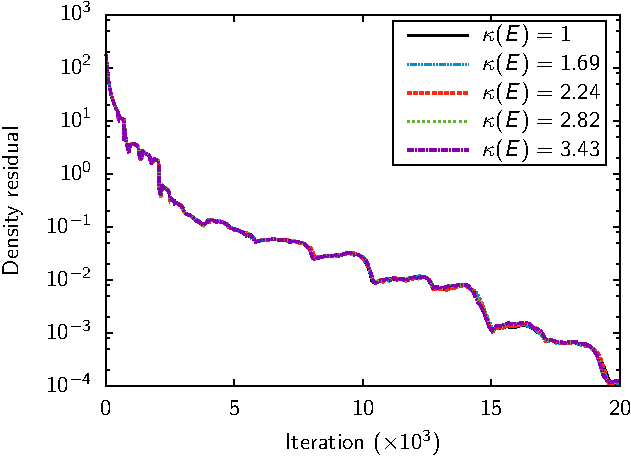
\includegraphics[width=.45\textwidth]{CANAL2_RESIDUAL_VS_CONDITIONNING_AMP001_PPT.pdf}}
  \subfigure[$a_1 = 0.05$]{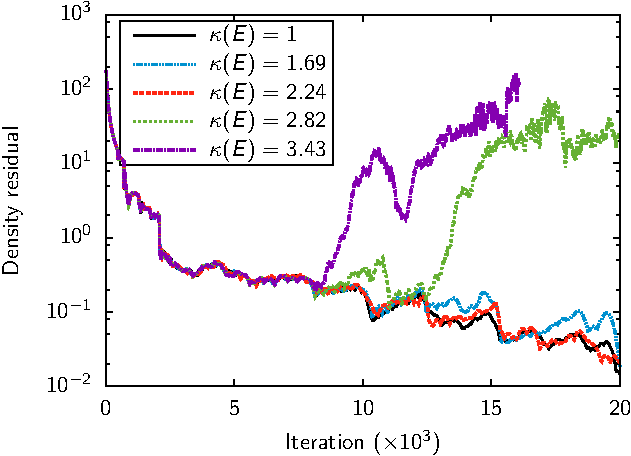
\includegraphics[width=.45\textwidth]{CANAL2_RESIDUAL_VS_CONDITIONNING_AMP005_PPT.pdf}}
  \caption{Relation between the condition number $\kappa (E)$ and the convergence of the solution.}
  \label{fig:canal_residual_vs_conditionning}
\end{figure}
The results in Fig.~\ref{fig:canal_residual_vs_conditionning} show that
for a condition number $\kappa (E) \geq 2.24$ and wave input amplitude
$a_1 = 0.05$, the computation diverges. However, the computations with
the same condition numbers but a smaller input amplitude $a_1 = 0.01$
converge. In fact, the condition number amplifies the errors made
during the iterative process. When the input waves have a smaller
amplitude, the iterative errors are slighter.

The problem is that for a given configuration, the amplitude of the computed unsteady phenomena can not
be \emph{a priori} known. This is emphasized in the section bellow
as in the literature, the condition number of the computations
has been almost $20$ and still the simulations converge.

\paragraph{Literature review}
\label{sec:condition_literature}

In the turbomachinery literature, \citet{Gopinath2007} and
\citet{Ekici2007} assessed their implementation of the
HB method on a 2D multi-stage compressor. 
It is composed of a rotor sandwiched by two stators having
32, 40 and 50~blades, respectively. Various combinations of the stators
blade passing frequencies are considered, 
but always with evenly-spaced time instances sampling the
largest period.  While \citet{Gopinath2007} use $2N+1$ samples (noted EVE $2N+1$),
\citet{Ekici2007} over-sample this period with $3N+1$ time instances
(noted EVE $3N+1$). This
leads to a rectangular $(2N+1)\times(3N+1)$ almost-periodic Fourier
matrix that gives thus HB computations that are more CPU and memory demanding
(see Sec.~\ref{sec:sm_hb_cost}). 
The chosen frequencies and the \emph{a posteriori}
associated condition numbers of the above references are given in
Tab.~\ref{tab:literature_multistage}.  
In bold text is highlighted the condition number used in the
original computations.
For $N=4$, the $3N+1$ instants
oversampling approach of \citet{Ekici2007} efficiently reduces the
condition number. But for this case, the use of evenly-spaced time
instances is sufficient as the condition number seems to be small enough
for the considered magnitude of unsteadiness.
\begin{table}
  \centering
  \begin{tabular}{rcc}
    \toprule
    \multicolumn{1}{c}{Reference} & \multicolumn{2}{c}{$\kappa(E)$} \\
    \multicolumn{1}{c}{and \# harmonics} & EVE $(2N+1)$ & EVE $(3N+1)$ \\
    \midrule
    \citet{Gopinath2007} ($N=2$) & $\mathbf{3.79}$ & $3.00$ \\
    \citet{Ekici2007} ($N=3$) & $5.40$ & $\mathbf{3.84}$ \\
    \citet{Gopinath2007} ($N=4$) & $\mathbf{11.25}$ & $2.07$ \\
    \citet{Gopinath2007} ($N=7$) & $\mathbf{16.66}$ & $14.61$ \\
    \bottomrule
  \end{tabular}
  \caption{Literature review of the condition number used in multi-frequential
  harmonic balance computations.}
  \label{tab:literature_multistage}
\end{table}

However, such an approach fails when dealing with configurations where:
\begin{itemize} \itemsep0pt \parskip0pt
  \item the amplitude of unsteadinesses is large as for instance
  large oscillations of a blade,
  \item the frequencies are widely segregated. In fact, as shown previously
  in Sec.~\ref{sec:condition_cror_ael}, the more segregated the frequencies, the
  higher the condition number using a uniform time sampling. This condition number
  can be tremendous ($\kappa (E) \ll 100$) preventing the use of such
  an approach for given configurations.
\end{itemize}

Moreover, as the amplitude of unsteadinesses plays a crucial role in
the amplification done by the condition number, the only
way to ensure that a simulation will converge is 
to minimize the condition number.
Therefore, the section below will be dedicated to
the development of algorithms to achieve this goal.


\section{Proposed cure: automatic optimization of time instances} % (fold)
\label{sec:condition_solution}
%!TEX root = ../../../adrien_gomar_phd.tex

Two algorithms that automatically choose the time instances in order to
minimize the condition number are presented: first, the Almost
Periodic Fourier Transform (APFT) algorithm, initially proposed in the
literature for electronics problems and implemented by
\citet{ThesisGuedeney} in his PhD thesis, is described, then a gradient-based
optimization algorithm over the condition number (OPT), developed in
the current work, is presented.

\subsection{Almost-Periodic Fourier Transform algorithm (APFT)}
\label{sec:apft_algorithm}
Based on the work of \citet{Kundert1988} in
electronics, the APFT
algorithm has been implemented by \citet{ThesisGuedeney} 
during his PhD thesis. The algorithm is designed
to maximize the orthogonality of the multi-frequential
IDFT matrix in order to minimize its condition number. To do so, a
Gram-Schmidt orthogonalization procedure is conducted.  First, the period 
associated with the smallest frequency ($2 \pi / \omega_{min}$) 
is oversampled with $M$ evenly spaced time
instances, $M\gg2N+1$ being specified by the user with $N$ the number of
frequencies. Considering these time instances, a rectangular
multi-frequential IDFT matrix is built. This rectangular matrix can be seen
as a set of $M$ vectors of length $2N+1$.
The first vector noted $V_0$ (corresponding
to $t=0$) is arbitrarily chosen as the first time instance and any
component in the direction of $V_0$ is removed from the following
vectors using the Gram-Schmidt formula
\begin{equation}
   V_s = V_s - \frac{V_0^\top V_s}{V_0^\top V_0} V_0, \quad s=1 \cdots M-1.
   \label{GramSchmidtAlgo}
\end{equation}
The remaining vectors are now orthogonal to $V_0$. 
Initially, the vectors had the same Euclidean norm.
Therefore, the vector that has now the largest norm is
the most orthogonal to $V_0$.
It is thus assigned to $V_1$. The previous
operations are then performed on the $M-2$ remaining vectors using $V_1$
as starting point. This process is repeated until the required $2N+1$ vectors
are defined. As a time instance corresponds to a vector, $2N+1$ time instances are obtained, 
which enables the construction of the multi-frequential
IDFT matrix. This algorithm is summarized in
Algo.~\ref{alg:algo_APFT}.

\begin{algorithm}
\caption{The Almost Periodic Fourier Transform Algorithm (APFT)}
\label{alg:algo_APFT}
\begin{algorithmic}
\STATE $\omega_{min} \leftarrow min \left( |\omega_k |,\quad 1 \leqslant k \leqslant N \right)$
\FOR{$m \leftarrow 0 \cdots M-1$}
    \STATE $t_m \leftarrow \displaystyle\frac{2\pi}{\omega_{min}}\frac{m}{M}$
\ENDFOR
\FOR{$n \leftarrow 1 \cdots 2N$}
   \FOR{$m \leftarrow n+1 \cdots M$}
  \STATE $ V_{m} \leftarrow V_{m} - \displaystyle\frac{V_{n}^\top \cdot V_{m}}{V_{n}^\top \cdot V_{n}} V_{n}$
   \ENDFOR
   \STATE \textbf{argmax()} returns the index of the largest member of a set
   \STATE $k=\textbf{argmax} \left( \| V_s^n \|,\quad n+1\leqslant s \leqslant M\right) $
   \STATE $\textbf{swap}(V_{n+1},V_{k})$
   \STATE $\textbf{swap}(t_{n+1},t_{k})$
\ENDFOR
\STATE $\mathbb{T}_{optimized} \leftarrow [t_0 \cdots t_{2N}]$
\end{algorithmic}
\end{algorithm}

\subsection{Gradient-based optimization algorithm (OPT)}
\label{sec:algo_opt}
A more direct approach is to seek directly a set of time instances
that minimize the condition number of the associated multi-frequential IDFT matrix. 
This minimization problem can be solved numerically by an optimization algorithm.

The limited memory optimization method of
\citet{Byrd1995} (noted L-BFGS-B) is
used to look for a minimum of the condition number of the
multi-frequential IDFT matrix $\kappa \left(E^{-1} \left[\mathbb{T} \right]
\right)$ as function of the time instances vector $\mathbb{T}$. This
quasi-Newton algorithm approximates the inverse Hessian matrix
$H(\kappa \left(E^{-1} \left[\mathbb{T} \right] \right))^{-1}$ with the
BFGS formula in order to decrease the objective $\kappa \left(E^{-1}
  \left[\mathbb{T} \right] \right)$ in the direction $-H(\kappa
\left(E^{-1} \left[\mathbb{T} \right] \right))^{-1}\nabla \kappa \left(E^{-1}
  \left[\mathbb{T} \right] \right)$. In the present case, the
derivative $\nabla \kappa \left(E^{-1} \left[\mathbb{T} \right] \right)$ of
the objective with respect to the time instances is approximated by
a first-order finite differences. The descent direction is
associated with the search for a zero of the gradient, which is a
necessary condition for an extrema, in a second-order Taylor series.
Finally, a line search on $\alpha$ is performed to minimize $\kappa
\left(E^{-1} \left[\mathbb{T} - \alpha H(\kappa \left(E^{-1} \left[\mathbb{T}
      \right] \right))^{-1} \nabla \kappa \left(E^{-1} \left[\mathbb{T}
      \right] \right) \right] \right)$.  An open-source implementation of this
broadly-used algorithm is
employed~\cite{Nocedal1980}.

Gradient descent methods being local, the L-BFGS-B method converges to a local
minimum of the condition number. This minimum is unsatisfying if the
starting time instances vector $\mathbb{T}$ is not well chosen, therefore a strategy
to find an appropriate initial point is required. To this aim, the smallest
angular frequency $\omega_{min}$ is used as a base angular frequency to create a set $\Omega$
\begin{equation}
    \Omega = [\frac{1}{M} \omega_{min} \cdots \frac{m+1}{M} \omega_{min} \cdots \omega_{min}],
    \label{eq:slitted_period}
\end{equation}
where $M$ denotes the desired number of initial guesses.
This gives a set of periods. Each of them are then evenly sampled to obtain a
set of time instances $\mathbb{T}_m$
\begin{equation}
    \mathbb{T}_m = \left[ 0, \frac{2 \pi M}{ (2N + 1) (m+1) \omega_{min}} \cdots 
                             \frac{2N \pi M}{ (2N + 1) (m+1) \omega_{min}} \right]
    \label{eq:set_of_tlv}
\end{equation}
These time instances sets are finally used as initial guesses for the
L-BFGS-B algorithm.

The multi-frequential IDFT matrix is then built for
each one of these time instances and the corresponding condition numbers are
computed. A large number $M$, typically thousands, of fractions of the
greatest period gives a large set of potential time instances vectors.
This is acceptable given the very low cost of the computation of the
condition number on such small matrices of size $(2N + 1) \times
(2N+1)$.  From this set, the time instances vector associated with the
multi-frequential IDFT matrix having the smallest condition number is
taken as a starting point.  The optimization algorithm actually achieves
a local adjustment of the time instances.

In this way, the exploitation capability of the gradient-based
optimizer is well combined with the exploration capacity of the
sampling. The OPT algorithm is summarized in Algo.~\ref{alg:algo_opt}.
\begin{algorithm}
\caption{The gradient-based optimization algorithm (OPT)}
\label{alg:algo_opt}
\begin{algorithmic}
\STATE $\omega_{min} \leftarrow min \left( |\omega_k |,\quad 1 \leqslant k \leqslant N \right)$
\FOR{$m \leftarrow 0 \cdots M - 1$}
    \STATE $\omega_m \leftarrow \frac{m + 1}{M} \cdot \omega_{min}$
    \FOR{$i \leftarrow 0 \cdots 2N$}
        \STATE $t_i \leftarrow \displaystyle\frac{i \cdot 2 \pi}{\omega_m \cdot (2N + 1)}$
    \ENDFOR
    \STATE $\mathbb{T}_m \leftarrow [t_0 \cdots  t_i \cdots t_{2N}]$
    \STATE $C_m \leftarrow \kappa \left(E^{-1} \left[\mathbb{T}_m \right] \right)$
\ENDFOR
\STATE \textbf{argmin()} returns the index of the smallest member of a set
\STATE $k \leftarrow \textbf{argmin}\left(C_m,\quad 0\leqslant m \leqslant M-1\right)$
\STATE $\textbf{min\_l-bfgs-b}\left(\kappa \left(E^{-1} \left[\mathbb{T}\right]\right), \mathbb{T}_{ini}\right)$ returns the optimal 
time instances vector $\mathbb{T}$ using the condition number $\kappa\left(E^{-1} \left[\mathbb{T}\right]\right)$ as objective function 
for the L-BFGS-B algorithm and  $\mathbb{T}_{ini}$ as starting point.
\STATE $\mathbb{T}_{optimized} \leftarrow 
  \textbf{min\_l-bfgs-b}\left(\kappa\left(E^{-1} \left[\mathbb{T}\right]\right), \mathbb{T}_{ini}=\mathbb{T}_k\right)$
\end{algorithmic}
\end{algorithm}

\subsection{Assessment of the algorithms}
Taking the same independent couple of frequencies $(f_1, f_2)$ as the one
used is Sec.~\ref{sec:condition_cror_ael}, the condition number of the
multi-frequential DFT matrix $\kappa (E)$ is computed, highlighting
the ability of the different algorithms to choose the time instances that
minimize the condition number, for any input frequencies. This
assessment is only made for two frequencies, but the results are similar
when increasing the number of frequencies. As two frequencies are
involved, five time instances are required. The results for the three
algorithms are depicted in Figure~\ref{fig:bench_algo}: (i)~APFT: the
Almost Periodic Fourier Transform algorithm, (ii)~OPT: the
gradient-based OPTimization algorithm and (iii)~EVE: EVEnly spaced
time instances oversampling the largest period as done in
\citet{Gopinath2007} using $2N+1$ time
instances and in \citet{Ekici2007} and \citet{Ekici2008} using $3N+1$
time instances.
Table~\ref{tab:algo_sum} gives some statistics about the results obtained
with each algorithm to give the reader a quantitative overview of the
efficiency of the different algorithms.
\begin{figure}[htp]
  \centering 
    \subfigure[EVE $(2N + 1)$]{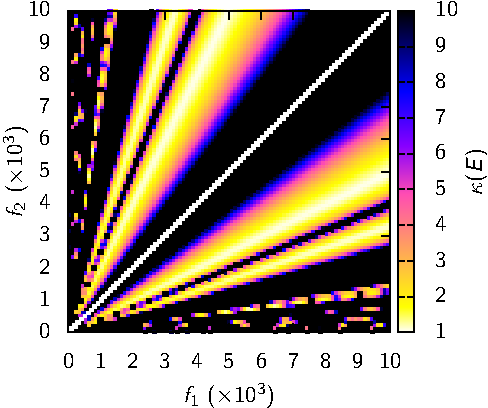
\includegraphics[width=.45\textwidth]{algo_equi_assessment.pdf}}
    \subfigure[EVE $(3N + 1)$]{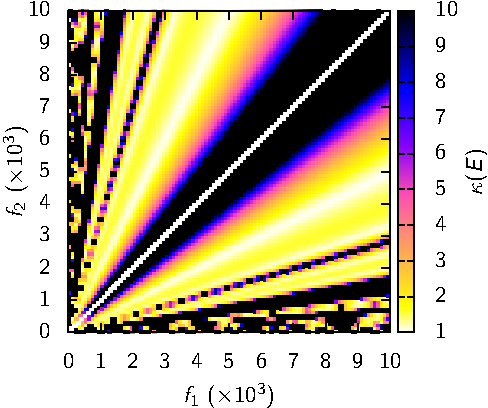
\includegraphics[width=.45\textwidth]{algo_equi_3n_assessment.pdf}}
    \subfigure[APFT]{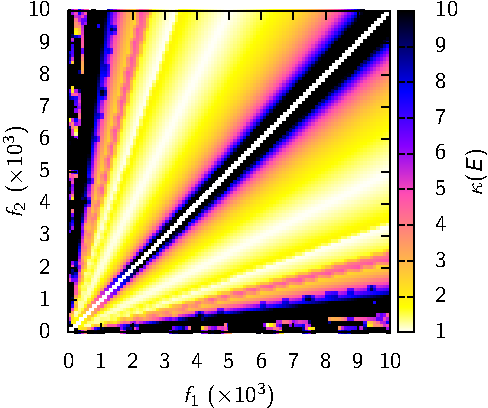
\includegraphics[width=.45\textwidth]{algo_apft_assessment.pdf}}
    \subfigure[OPT]{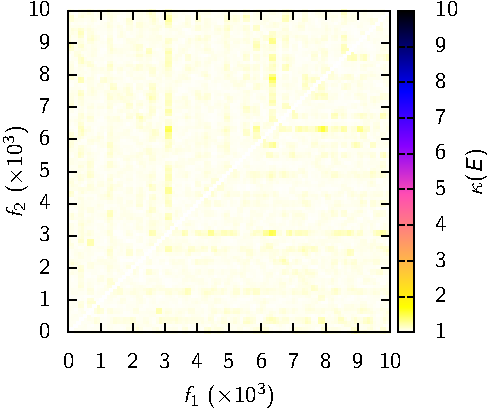
\includegraphics[width=.45\textwidth]{algo_opt_assessment.pdf}}
  \caption{Condition number of the discrete Fourier transform matrix $E$
  using two independent frequencies and four different algorithms
  to choose the time instances.}
  \label{fig:bench_algo}
\end{figure}

The EVE algorithms give fair results ($\kappa(E) \leq 2$) only at
discrete couples of frequencies, corresponding 
to the particular cases where $f_2$ is a
multiple of $f_1$, as shown in Sec.~\ref{sec:condition_cror_ael}. 
This is not promising as these
cases can be computed using the mono-frequential formulation and thus does not
need non-uniform time instances. Oversampling improves the results. 
In fact, the mean condition number obtained
with $3N + 1$ samples indicates that the higher the number of time instances
the better the condition number. However the multi-frequential DFT
matrix becomes rectangular. The memory and CPU cost being proportional to 
the number of time instances (see Sec.~\ref{sec:sm_hb_cost}), 
such a strategy can not be
used in an industrial context. The APFT
algorithm improves the results, as it gives $\kappa (E) \leq 2$ 
for a large interval but fails when the frequencies
are too close from one another ($f_1 \approx f_2$) or when they are significantly
different ($f_1 \ll f_2$ or $f_1 \gg f_2$).  
Finally, the OPT algorithm gives a condition number close to unity for
all couple of frequencies $(f_1, f_2)$. Moreover, the OPT algorithm is
the only one to give a standard deviation that is smaller than the mean,
proving its robustness.
\begin{table}[htp]
  \ra{1.3} 
  \centering
  \begin{tabular}{lcccc}
    \toprule
    \phantom{abdefghijk} & min & max & mean & $\sigma$ \\
    \midrule
    EVE ($2N + 1$) & $1.0$ & $9.4\e{16}$ & $1.5\e{14}$ & $2.8\e{15}$ \\
    EVE ($3N + 1$) & $1.0$ & $3.7\e{16}$ & $4.7\e{13}$ & $9.5\e{14}$ \\
    APFT & $1.0$ & $81.2$ & $5.9$ & $9.0$ \\
    OPT & $1.0$ & $2.6$ & $1.1$ & $7.7\e{-2}$ \\
    \bottomrule
  \end{tabular}
  \caption{Condition number of the discrete Fourier transform matrix $E$
  statistics for two independent frequencies using four different algorithms
  to choose the time instances.}
  \label{tab:algo_sum}
\end{table} 

The configurations encountered in the turbomachinery literature 
are taken again to demonstrate the capability of the presented
algorithms to minimize the condition number
regardless of the input frequencies. The results are shown in 
Tab.~\ref{tab:literature_multistage2}.
The APFT algorithm improves the condition number compared to the
EVE ($2N+1$) but can give relatively large condition numbers, here $12.95$. 
In opposite, the OPT algorithm developed in the
present contribution gives results close to one for the four configurations.
\begin{table}[htp]
  \ra{1.3} \centering
  \begin{tabular}{rcccc}
    \toprule
    \multicolumn{1}{c}{Reference} & \multicolumn{4}{c}{$\kappa(E)$} \\
    \multicolumn{1}{c}{and \# harmonics} & EVE $(2N+1)$ & EVE $(3N+1)$ & APFT & OPT \\
    \midrule
    \citet{Gopinath2007} ($N=2$) & $\mathbf{3.79}$ & $3.00$ & $1.72$ & $1.08$ \\
    \citet{Ekici2007} ($N=3$) & $5.40$ & $\mathbf{3.84}$ & $1.71$ & $1.00$ \\
    \citet{Gopinath2007} ($N=4$) & $\mathbf{11.25}$ & $2.07$ & $3.46$ & $1.13$ \\
    \citet{Gopinath2007} ($N=7$) & $\mathbf{16.66}$ & $14.61$ & $12.95$ & $1.00$ \\
    \bottomrule
  \end{tabular}
  \caption{Literature review of the condition number used in multi-frequential
  harmonic balance computations compared to the presented algorithms.}
  \label{tab:literature_multistage2}
\end{table}

% Thus the proposed non-uniform time sampling combined with the OPT
% algorithm allows to tackle problems with large frequency
% separation. In such cases, the gain of the HB approach compared
% to classical time-marching methods is expected to be significant: with
% a time-marching scheme, the time-step has to be small enough to
% discretize the shortest period, while the number of time steps of the
% simulation has to be long enough to reach the steady-state
% (\emph{i.e.}  the simulation time is equal to several
% times the longest period). Conversely, as detailed in Sec.~\ref{sec:sm_hb_cost},
% the cost of the HB method only
% depends on the number of frequencies to capture, regardless of their
% relative values.

Thus, the non-uniform time sampling proposed by \citet{ThesisGuedeney}
used together with the OPT algorithm developed in the present contribution
enables to tackle problems with large frequency separation and/or large unsteadinesses,
namely CROR aeroelasticity.

\subsection{Distribution of the time instances}
For harmonically-related frequencies, the set of time instances
that minimize the condition number is 
provided by a uniform sampling of the fundamental frequency period
as it gives the theoretical lower bound $\kappa (E) = 1$. Since the
frequencies are harmonically related, the distribution of the time
instances on the other frequencies is also uniform. 
In fact, considering the
frequency vector $F = \left[f_1 \cdots f_k= kf_1 \cdots Nf_1 \right]$
and the time instances vector
$\mathbb{T}$ uniformly sampling the smallest frequency
\begin{equation}
  \mathbb{T} = \left[0, \frac{1}{f_1 (2N+1)} \cdots  \frac{2N}{f_1 (2N+1)} \right],
  \label{eq:evenly_spaced_timelevels}
\end{equation}
then the product of the $i^{th}$ term of $\mathbb{T}$ to its
associated frequency is
\begin{equation}
  f_1 \frac{i}{f_1 (2N+1)} = k f_1 \frac{i}{k f_1 (2N+1)} = f_k \frac{i}{f_k (2N+1)}.
  \label{eq:evenly_spaced_timelevels_2}
\end{equation}
Equation~\eqref{eq:evenly_spaced_timelevels_2} means that evenly-spaced
time instances for the fundamental frequency are still seen as evenly
spaced by the $k^{th}$ harmonic. This is an explanation why the
condition number of the multi-frequential IDFT matrix $E^{-1}$ will be
unity as each frequency is sampled by evenly spaced time
instances~\cite{Brambilla1999}.

Now, considering non-harmonically related frequencies, there is
mathematically no reason for evenly-spaced time instances over the
smallest frequency to be seen as evenly spaced by the other frequencies
in general.

Figure~\ref{fig:distribution_tlv} shows the distribution of the time
instances, relative to each frequency period, obtained by the presented
algorithms for the frequencies $f_1 = 3$~Hz and $f_2 = 17$~Hz. 
To do so, the chosen time instances are redistributed
on the considered frequency period by applying a modulo to it
\begin{equation}
  \label{eq:1}
  \mathbb{T}^{[f_k]}_j =  \mathbb{T}_j \text{ modulo } 1/f_k
\end{equation}
Then, they are divided by the latter, so that the results are
dimensionless.  In light gray line is depicted the $y=x$ function
representing the evenly-spaced solution on the considered period.
Keeping in mind that if each frequency sees evenly-spaced time instances,
then the condition number is the smallest, the optimal solution would
be to have relative time instances on $y=x$ for each period.  Running the
EVE $(2N + 1)$, APFT and OPT algorithms leads to a condition number of $33.1$,
$3.8$ and $1.1$, respectively.  The EVE algorithm gives a perfect distribution
of the time instances with respect to
period $1/f_1$ as the time instances are sampled on the period
$1/f_1$. However, it gives results that are far from the evenly spaced time instances
within period $1/f_2$. The APFT algorithm is nowhere near the evenly spaced
solution for both the considered periods, but closer than EVE regarding
period $1/f_2$. Finally, the OPT algorithm is the only one to be close
to the evenly spaced solution for each period considered. This explains the
very good condition numbers obtained with the OPT algorithm.
\begin{figure}[htp]
  \centering 
  \subfigure[relative to period $1/f_1$]{
      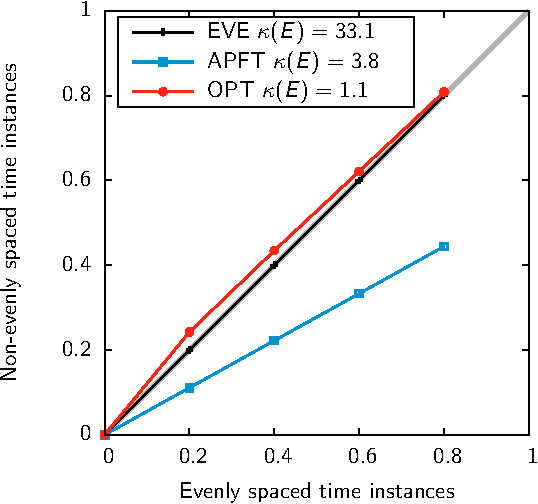
\includegraphics[width=.45\textwidth]{timelevels_distribution_f1.pdf}}
  \subfigure[relative to period $1/f_2$]{
      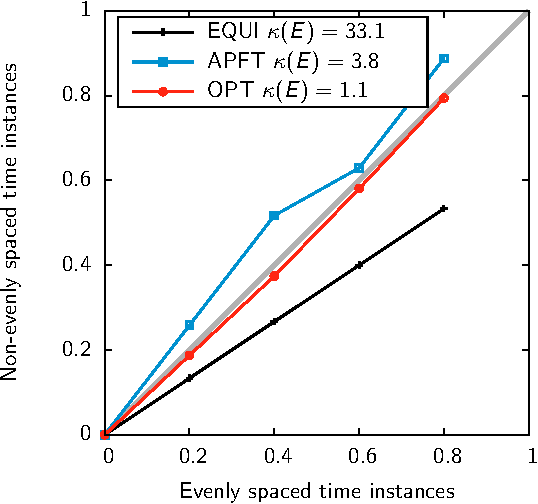
\includegraphics[width=.45\textwidth]{timelevels_distribution_f2.pdf}}
  \caption{Distribution of the time instances on each frequency periods.}
  \label{fig:distribution_tlv}
\end{figure}


% \section*{Summary}

% We have seen that the condition number of the
% discrete Fourier transform matrix $E$ can be large
% when using the multi-frequential framework. The present work,
% namely contra-rotating open rotor aeroelasticity, is
% by essence multi-frequential. It has been shown that in this context,
% the condition number has to be minimize for the harmonic balance
% computations to converge and the results to be reliable. 
% To ensure that, non-uniform time instances
% are used together with the OPT algorithm that provides an
% optimal condition number for any input frequencies.

%!TEX root = ../../../adrien_gomar_phd.tex

\chapter{Convergence of Fourier-based 
time methods for turbomachinery wake passing problems}
\label{cha:limitations_convergence}

\chabstract{Efficiency of the HB method results from a trade-off between accuracy and 
costs requirements.
On one hand, the accuracy of Fourier-based time methods depends on the number of harmonics
used to represent the frequency content of the time signal; on the other
hand, computational costs and memory consumption of the computations also scale
with the number of harmonics. Theoretical results about the convergence of spectral methods 
(see e.g. Canuto~\emph{et al.}~\cite{Canuto2006}
for a comprehensive review) predict convergence of the numerical 
solution starting from a given number of harmonics, provided 
that the approximated function satisfies some regularity 
requirements~\cite{Zygmund1959}. 
Nevertheless, this number of harmonics is configuration-dependent 
and hardly predictable. In this work, we focus on turbomachinery 
configurations, which involve flow across a series of fixed and 
rotating bladed wheels. Studies on the convergence of 
Fourier-based time methods for turbomachinery simulations 
have been previously reported in the literature, but with scattered results. 
For instance, using a frequency-domain approach, 
Vilmin~\emph{et al.}~\cite{Vilmin2006} obtain accurate solutions 
using 5~harmonics for a compressor stage and 3~harmonics for a 
centripetal turbine stage. For a transonic compressor stage with 
forced blade vibration, Ekici~\emph{et al.}~\cite{ekici2010} use 
up to 7~harmonics with a time-domain harmonic balance approach. Finally, for a 
subsonic compressor stage, Sicot~\emph{et al.}~\cite{JSicot2012} report 
that 4~harmonics is the minimal requirement to properly capture wake interactions
as illustrated in Fig.~\ref{fig:cme2}. 
\begin{figure}[htb]
  \centering
  \subfigure[reference unsteady si\-mu\-lation]{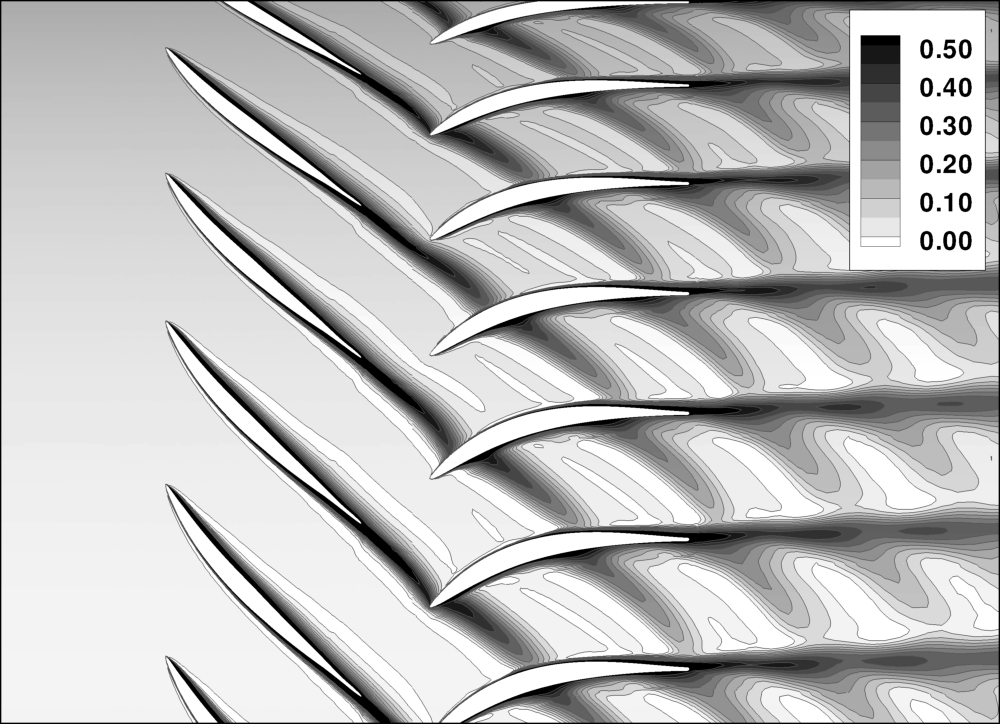
\includegraphics[width=.3\textwidth]{uransentropie_nb.jpg}}
  \subfigure[HB $N=2$]{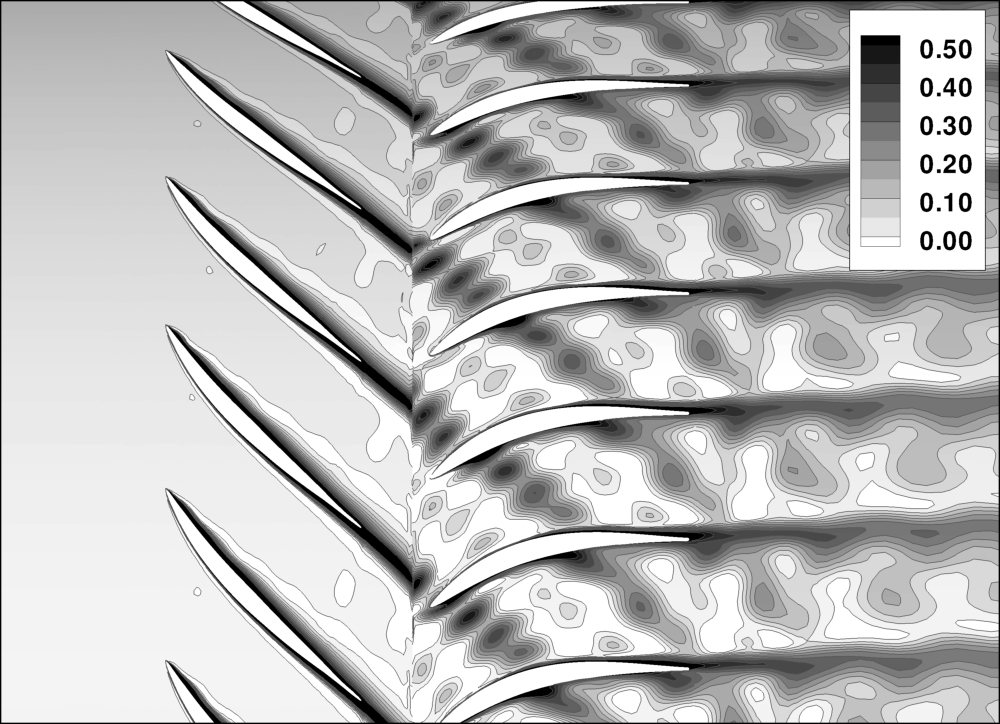
\includegraphics[width=.3\textwidth]{n2_entropie_nb.jpg}}
  \subfigure[HB $N=3$]{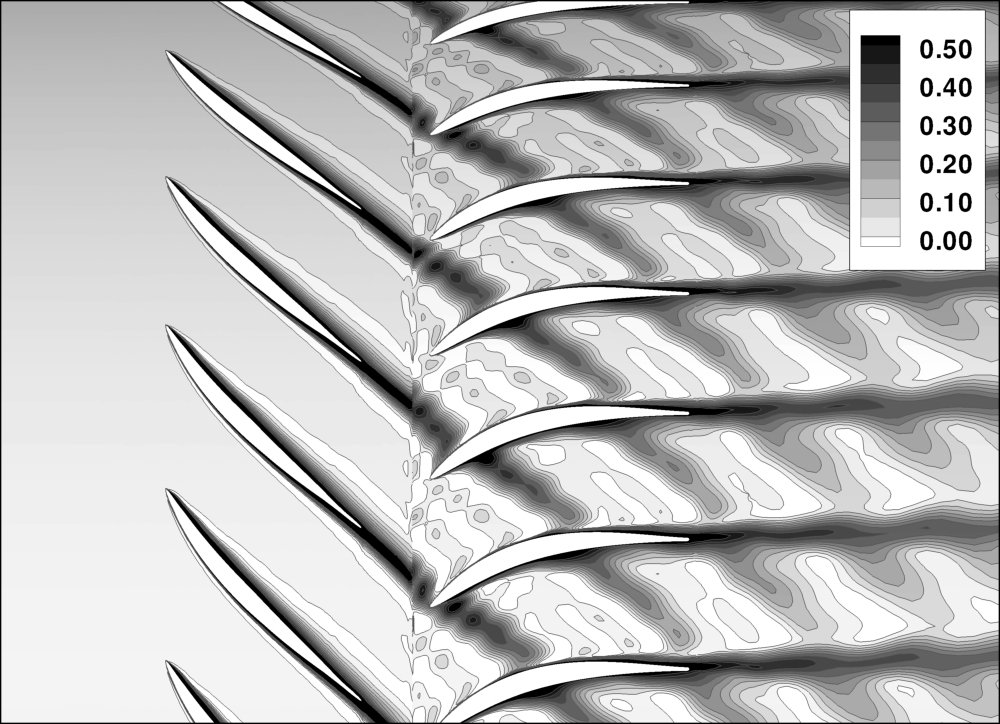
\includegraphics[width=.3\textwidth]{n3_entropie_nb.jpg}}
  \subfigure[HB $N=4$]{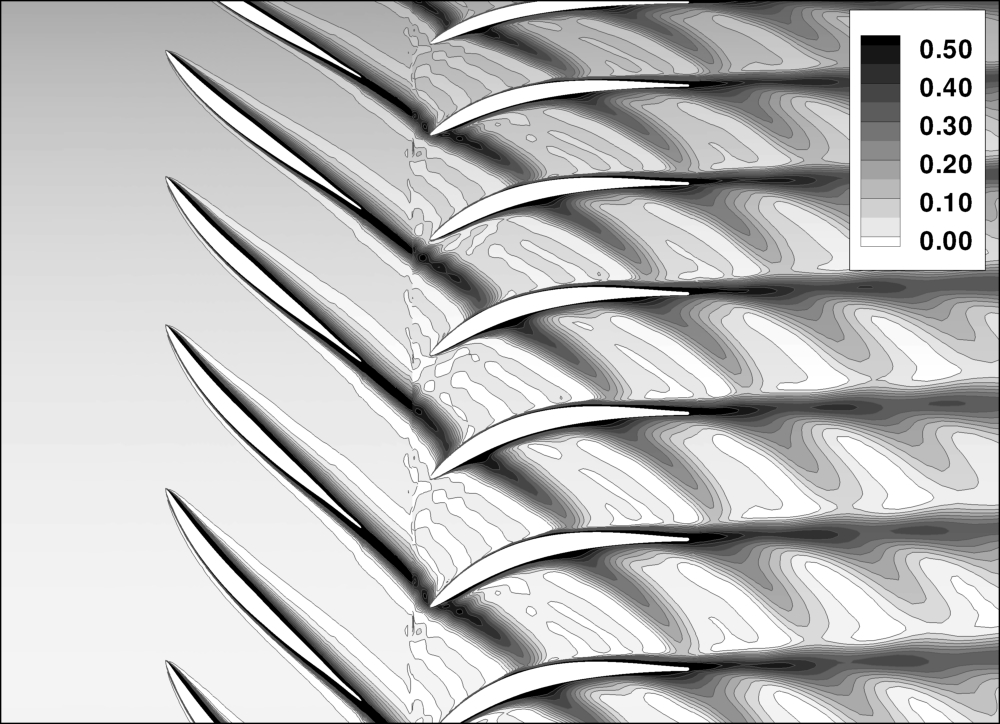
\includegraphics[width=.3\textwidth]{n4_entropie_nb.jpg}}
  \subfigure[HB $N=5$]{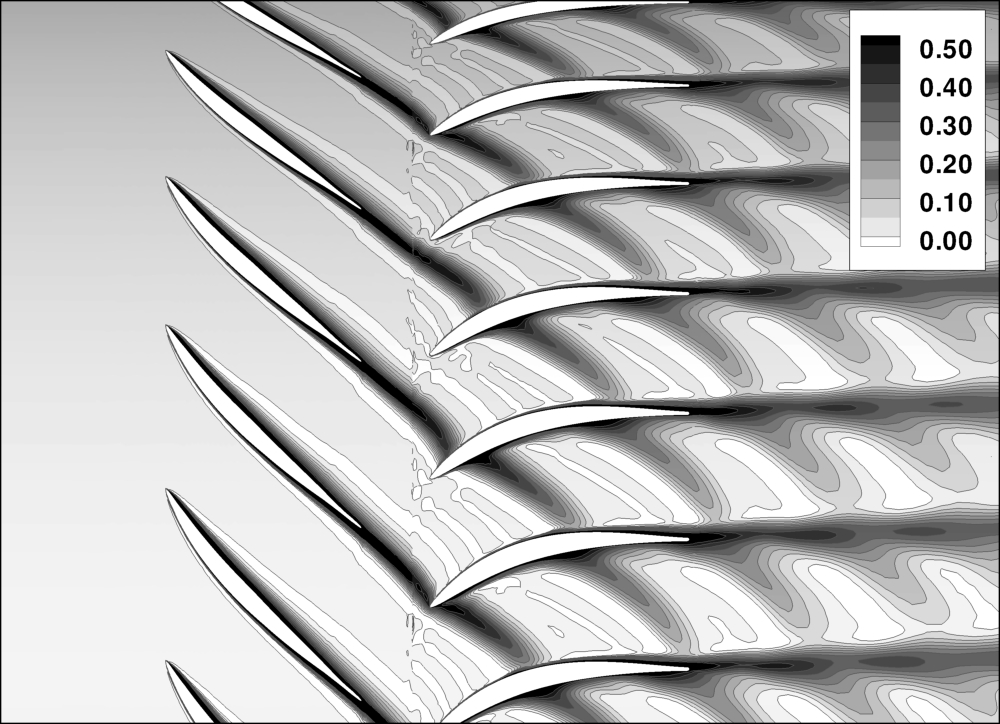
\includegraphics[width=.3\textwidth]{n5_entropie_nb.jpg}}
  \subfigure[HB $N=6$]{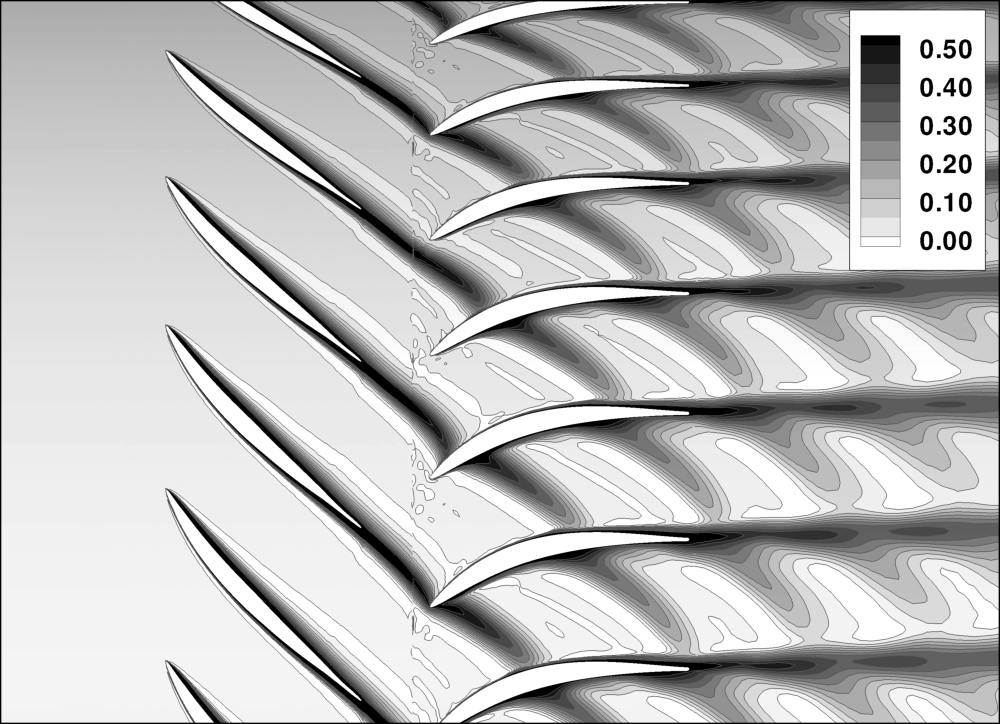
\includegraphics[width=.3\textwidth]{n6_entropie_nb.jpg}}
  \caption{Convergence of harmonic balance computations for a rotor/stator configuration from \citet{JSicot2012}.}
  \label{fig:cme2}
\end{figure}

The preceding examples show that no consensus exists in the literature 
concerning the number of harmonics needed to achieve convergence,
even for similar configurations.
The goal of the present paper is twofold: to analyze the
convergence of Fourier-based time method, with focus on turbomachinery applications, 
and to provide a criterion for the minimal number of harmonics 
required to achieve a specified accuracy level. The paper is organized as follows: first,
we recall the design principles of the time-domain harmonic balance 
approach and theoretical results about the convergence of Fourier-based methods.
Second, the HB method is applied to the linear advection equation 
supplemented with unsteady boundary conditions of different degrees of smoothness,
to highlight the impact of solution regularity on HB convergence. 
Third, a model problem representative of a turbomachinery wake-passing 
configuration is set up, and different
error measures are introduced to compare the numerical and analytical solutions. 
These error measures allows finally to define a prediction tool, 
which is applied to contra-rotating open rotor simulations.
}

\minitoc
\newpage

\section{Linear advection of a periodic perturbation}
\label{sec:convergence_advection}
%!TEX root = ../../../adrien_gomar_phd.tex

In this section, the linear advection toy problem is used
with two different input functions to highlight the convergence
properties of the HB approach retained in this PhD thesis.

\subsection{Rectangular function}

In fluid dynamics, the simplest model 
representative of a shock wave
is the step function.
The periodic step function over the period $T=1/c$ is defined as:
\begin{equation}
    u_l(t) = 
    \begin{cases}
        0, & \text{if } 0 \leq t < \frac{T}{2}, \\
        1, & \text{if } \frac{T}{2} \leq t < T.
    \end{cases}
    \label{eq:inject_step}
\end{equation}

\begin{figure}
  \centering
  \subfigure[$N=1$]{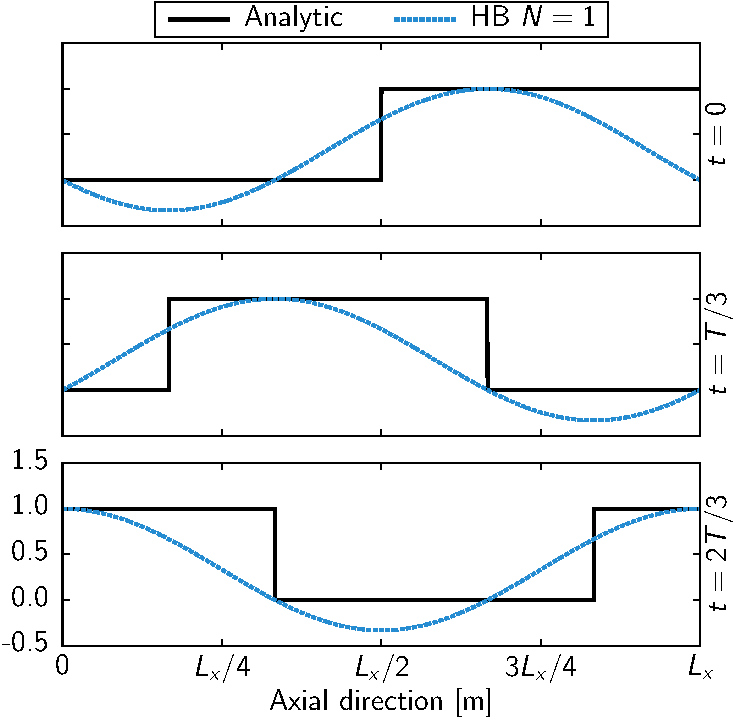
\includegraphics[width=.35\textwidth]{convection_step_N1.pdf}}
  \subfigure[$N=2$]{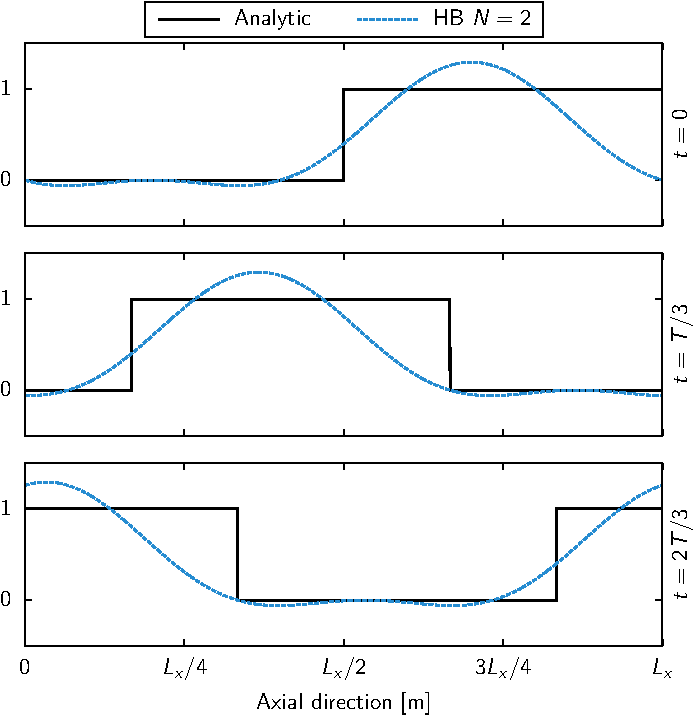
\includegraphics[width=.35\textwidth]{convection_step_N2.pdf}}
  \subfigure[$N=3$]{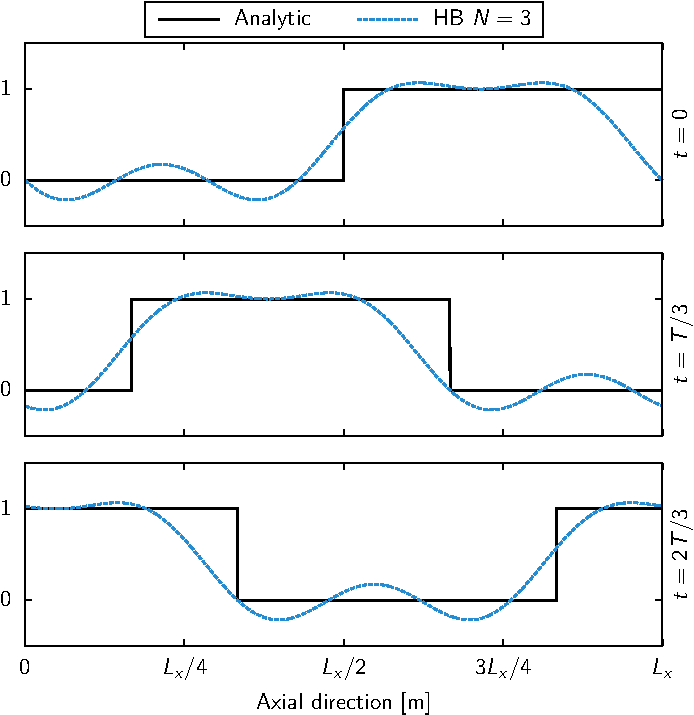
\includegraphics[width=.35\textwidth]{convection_step_N3.pdf}}
  \subfigure[$N=4$]{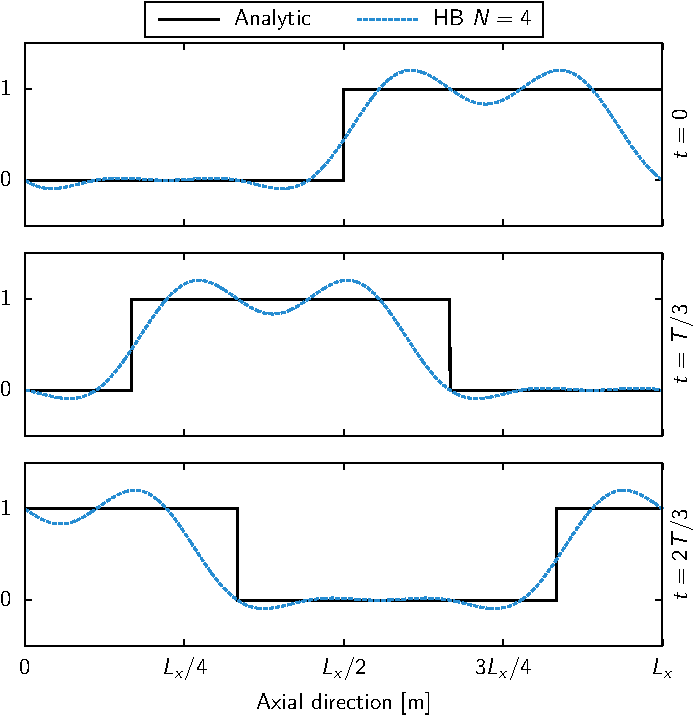
\includegraphics[width=.35\textwidth]{convection_step_N4.pdf}}
  \subfigure[$N=5$]{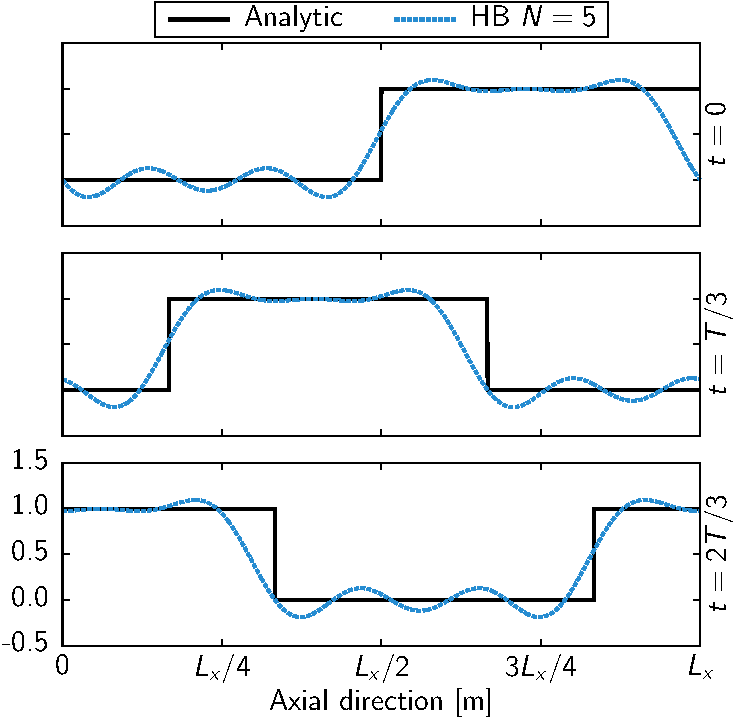
\includegraphics[width=.35\textwidth]{convection_step_N5.pdf}}
  \subfigure[$N=6$]{\includegraphics[width=.35\textwidth]{convection_step_N6.pdf}}
  \caption{Linear advection of a rectangular function: 
  numerical solutions at different time instances for different numbers of harmonics.}

  \label{fig:inj_step_results}
\end{figure}

Figure~\ref{fig:inj_step_results} depicts the results of HB computations
using one to six harmonics at different time instances. The convergence rate 
is slow, and for the six-harmonics HB computation the
shape of the rectangular function is still barely captured. 
The well-known \citet{Gibbs1899}
phenomenon is observed, which is a typical drawback 
of Fourier-based methods applied to discontinuous problems, 
see e.g. \citet{Canuto2006}.

\begin{figure}
  \centering
  \includegraphics[width=.5\textwidth]{convection_step_error.pdf}
  \caption{Linear advection of a rectangular function: convergence of the HB method error.}
  \label{fig:conv_step}
\end{figure}
As for the previous case, the $\mathcal{L}_2$-norm 
of the error is depicted in Fig.~\ref{fig:conv_step}. 
The convergence of the sum of sine functions, that has been studied in Sec.~\ref{sec:sum_sine},
is added for comparison.
The convergence rate is dramatically different from the previous one: 
the error decreases slowly when more harmonics are introduced, 
but the exact solution is never reached, 
unless an infinite number of harmonics is considered.

The discrete Fourier transform of the results
is computed and compared to the analytical result in Fig.~\ref{fig:dft_step}.
For this case, the spectrum in not finite and cannot be captured accurately
with a finite number of samples.

\begin{figure}
  \centering
  \includegraphics[width=.5\textwidth]{convection_step_dft.pdf}
  \caption{Linear advection of a rectangular function: 
  discrete Fourier transform.}
  \label{fig:dft_step}
\end{figure}

\FloatBarrier

\subsection{Toward turbomachinery wakes}
\label{sec:turbomachine_wake}

Consider for simplicity a turbomachinery stage composed of two rotors,
as for instance a CROR configuration.
A wake is shed behind
the upstream and the downstream rotor. 
It is stationary in the frame of reference attached to the upstream wheel.
\begin{figure}
    \centering\includegraphics[width=.35\textwidth]{cror_wakes.pdf}
  \caption{Characteristic wakes in a CROR configuration.}
  \label{fig:rotor-stator}
\end{figure}
However, when it crosses the rotor-rotor interface,
the wake becomes unsteady in the frame of reference of the second wheel. 
Thus, an upstream steady spatial distortion becomes unsteady in
the downstream row.

Thus, in the downstream reference frame, wakes coming 
from the upstream wheel can be represented, 
to a first approximation, as the periodic 
advection of a Gaussian function from the inter-wheel interface.

We consider again the linear advection toy problem (see Sec.~\ref{sec:toy_convection}), 
with $u_l$ now taken equal to a Gaussian function following the
\citet{Lakshminarayana1980} similarity law:
\begin{equation}
    u_l (t) = u_m \left[1 - 
        \Delta u \cdot e^{
          -0.693 \left(\frac{2 c t}{L_x L} \right) ^ 2}\right],
\end{equation}
The full width at half maximum $L$ of the wake is set to 10\% of the domain size, 
$u_m$ is set to $c$ and $\Delta u$ to 10\% of $u_m$.

\begin{figure}
  \centering
  \subfigure[$N=1$]{\includegraphics[width=.35\textwidth]{convection_wake_N1.pdf}}
  \subfigure[$N=2$]{\includegraphics[width=.35\textwidth]{convection_wake_N2.pdf}}
  \subfigure[$N=3$]{\includegraphics[width=.35\textwidth]{convection_wake_N3.pdf}}
  \subfigure[$N=4$]{\includegraphics[width=.35\textwidth]{convection_wake_N4.pdf}}
  \subfigure[$N=5$]{\includegraphics[width=.35\textwidth]{convection_wake_N5.pdf}}
  \subfigure[$N=6$]{\includegraphics[width=.35\textwidth]{convection_wake_N6.pdf}}
  \caption{Linear advection of a Gaussian function representing a turbomachinery wake: 
  numerical solutions at different time instances for different numbers of harmonics.}
  \label{fig:inj_wake_results}
\end{figure}
Figure~\ref{fig:inj_wake_results} depicts the HB
computations for one to six harmonics. The numerical solution convergences
to the exact Gaussian function starting from $N=6$ harmonics.
When the number of harmonics is
too small, the width and the depth of the wake are badly approximated
by the method, and the solution exhibits some spurious oscillations. 

\begin{figure}
  \centering
  \includegraphics[width=.5\textwidth]{convection_wake_error.pdf}
  \caption{Linear advection of a Gaussian function representing a 
  turbomachinery wake: convergence of the HB method error.}
  \label{fig:conv_wake}
\end{figure}
Figure~\ref{fig:conv_wake} shows the quantitative convergence of 
the $\mathcal{L}2$ error. The
convergence curves for the two functions studied in the previous sections
are also reported for comparison.
The error follows now a nearly exponential convergence.
\begin{figure}
  \centering
  \includegraphics[width=.5\textwidth]{convection_wake_dft.pdf}
  \caption{Linear advection of a Gaussian function representing a turbomachinery wake: 
  discrete Fourier transform.}
  \label{fig:dft_wake}
\end{figure}
The discrete Fourier transform of the results is
depicted against the analytical result in Fig.~\ref{fig:dft_wake}.
The $N=2$ and $N=4$ computations badly capture the amplitudes of the
resolved harmonics.
Starting from $N=6$, some of the lower 
frequencies are correctly captured, whereas high frequencies are
always under-estimated.
This improves when further harmonics are added to the computation.

For a better understanding of the HB convergence behavior, 
we consider the spectral content of the Gaussian wake model. 
Precisely, the Fourier transform $\widehat{g}$ of a Gaussian function $g$
defined as:
\begin{equation}
    g(x) = A e^{-\alpha x^2},
    \label{eq:simple_gaussian_function}
\end{equation}
where $A$ and $\alpha$ are constants, is:
\begin{equation}
    \widehat{g}(f) = A^\prime e^{-\alpha^\prime f^2},
    \label{eq:fourier_transform_gaussian}
\end{equation}
where:
\begin{equation}
  \begin{cases}
    A^\prime=A \sqrt{\frac{\pi}{\alpha}},\\
    \alpha^\prime = \frac{\pi^2}{\alpha}.
  \end{cases}
\end{equation}

For the similarity law of Lakshminarayana and Davino, 
$\alpha$ and $\alpha^\prime$ can be identified as:
\begin{equation}
    \alpha =  0.693 \left( \frac{2}{L} \right)^2, \quad
    \alpha^\prime =  \frac{1}{0.693} \left( \frac{\pi L}{2} \right)^2.
    \label{eq:gaussian_params_laksh}
\end{equation}
The exponential factor of the wake law~$\alpha$ is inversely
proportional to its Fourier counter-part~$\alpha'$, meaning that their
width will vary in opposite way: the thinner the wake, the wider its
spectrum and vice-versa.

The convergence rate is inherently linked to
the spectrum of the considered unsteady signal.
As for the present case we know the analytical wake spectrum,
we define the theoretical truncation error as the ratio of
the energy contained in the unresolved part 
of the spectrum to the overall energy content of the full spectrum:
\begin{equation}
    \varepsilon_{th}(f) = \sqrt{\frac{
        \int_f^\infty | \widehat{g}(\zeta)|^2 \diff \zeta
      }{
        \int_0^\infty | \widehat{g}(\zeta)|^2 \diff \zeta
      }}.
    \label{eq:def_truncation_error}
\end{equation}
Introducing the error function defined as:
\begin{equation}
    \erf(x) = \frac{2}{\sqrt{\pi}} \int_0^x e^{-t^2} \diff t,
\end{equation}
and the complementary error function defined as:
\begin{equation}
    \erfc(x) = 1 - \erf(x),
\end{equation}
then:
\begin{align}
    \int_0^\infty | \widehat{g}(\zeta)|^2 \diff \zeta 
    &= \frac{1}{2} \int_{- \infty}^\infty | \widehat{g}(\zeta)|^2 \diff \zeta \\
    &= \frac{A^{\prime 2}}{2} \sqrt{\frac{\pi}{2 \alpha^\prime}},
\end{align}
and:
\begin{equation}
    \int_f^\infty | \widehat{g}(\zeta)|^2 \diff \zeta = 
      \frac{A^{\prime 2}}{2} \sqrt{\frac{\pi}{2 \alpha^\prime}} \erfc (\sqrt{2 \alpha^\prime} f).
\end{equation}
The theoretical truncation error can then be written as:
\begin{equation}
    \varepsilon_{th}(f, L) = \sqrt{\erfc (\sqrt{2 \alpha^\prime(L) } f)}.
    \label{eq:analytical_conv}
\end{equation}
One can notice from Eq.~\eqref{eq:analytical_conv} that the 
truncation error does not depend on the wake deficit $\Delta u$ 
but only on the wake width $L$.

\begin{figure}
    \centering\includegraphics[width=.6\textwidth]{ANALYTICAL_ERROR_PPT.pdf}
  \caption{Theoretical truncation error of the Lakshminarayana and Davino wake law.}
  \label{fig:analytic_error_paper}
\end{figure}
Eq.~\eqref{eq:analytical_conv} is depicted in
Fig.~\ref{fig:analytic_error_paper}. 
It can be seen that the wider the spectrum,
the higher the number of harmonics needed to
reach a certain level of error. 
Moreover, for a thin wake width (e.g. 2\% of the pitch)
the number of harmonics required to capture it with a truncation 
error of 10\% is up to 25~harmonics.
In the limit of $L \to 0$, the wake becomes a Dirac function
which represents the worst possible case.
In the preceding example, the Gaussian function had a width
of 10\% which, according to Eq.~\eqref{eq:analytical_conv},
is captured by using $N=7$ harmonics for a target 10\% error.

\section{Application to a model turbomachinery configuration}
\label{sec:rotating_blocks}
%!TEX root = ../../../adrien_gomar_phd.tex


\subsection{Extension of the harmonic balance approach to
  turbomachinery computations}
\label{sec:turbomachinery_adaptation}

To efficiently apply the HB approach to turbomachinery
configurations, phase-lag boundary conditions~\cite{Erdos1977} are
used to cut down the mesh size by using a grid that spans only one
blade passage per row. The phase-lag boundary conditions are two-fold:
i) the azimuthal boundaries of a passage and ii) the blade row
interface which must handle different row pitches on either
sides. Furthermore, in the HB framework, each row captures the blade
passing frequency of the opposite row leading to different time
samplings solved in each row.

The phase-lag condition is based on the space-time periodicity of the
flow variables. It states that the flow in one passage~$\theta$ is the
same as the next passage~$\theta+\Delta\theta$ but at another
time~$t+\delta t$:
\begin{equation}
  W\left(\theta+\Delta\theta,t \right) = W\left(\theta,t+\delta t \right),
  \label{eq:choro}
\end{equation}
where $\Delta \theta$ is the pitch of the considered row.  The time
lag $\delta t$ can be expressed as the phase of a rotating wave
traveling at the same speed as the relative rotation speed of the
opposite row: $\delta t=\beta/\omega_\beta$.  The Inter-Blade Phase
Angle $\beta$ (IBPA) depends on each row blade count and relative
rotation speed. It is analytically given \citet{Gerolymos1991}.  The Fourier
transform of Eq.~\eqref{eq:choro} implies that the spectrum of the
flow in a passage is equal to the spectrum of the neighbor passage
modulated by a complex exponential depending on the IBPA:
\begin{equation*}
%  \label{eq:serfourphasetemps}
  \widehat{W}_k(x, r,  \theta+\theta_G)  = {\widehat{W}_k(x, r,
    \theta)e^{i k\beta}}.
\end{equation*}
At the azimuthal boundaries, this modulation can be computed on the fly
in the HB framework as a sampling of the time period is always known
and it is straightforward to derive an analytic derivation in the time
domain (see Ref.~\cite{JSicot2012}). The blade row interface is more complex
as the different pitches and relative motion of the rows require to
duplicate the flow in the azimuthal direction using the phase-lag
periodicity. A time interpolation also occurs to take the
different time samplings into account and a non-abutting mesh
technique is applied as the mesh will unlikely have matching
cells. To remove spurious waves, an over-sampling and a filtering are
performed. 

The time-domain harmonic balance method has been implemented 
by CERFACS in the
\emph{elsA} solver~\cite{Cambier2013} developed by ONERA. 
This code solves the RANS equations using a cell-centered
approach on multi-blocks structured meshes.  Using the HB method,
significant savings in CPU cost have been observed in various
applications such as rotor/stator interactions~\cite{JSicot2012}
and dynamic derivatives computation~\cite{CIHassan2011}. 


\subsection{Spectral convergence study}
The primary interest in this section is the wake capturing capabilities of the 
Fourier-based time method in the rotating part. 
To analyze this, two error measures are defined and
evaluated. 

\subsubsection{Spatial-spectrum based error measure}
\label{sec:crit_1}
Initially, we propose an error measure ($\varepsilon_1$) based 
on the loss of signal energy
induced by the harmonic method at the interface. 
In fact, in the stator part, the wake is steady and is thus not
filtered by the HB operator. 
Conversely, in the rotor part, the steady wake becomes
unsteady due to the relative speed difference between the
stator and the rotor. However, only a finite number of harmonics~$N$
is used to describe the unsteady field, hence the filtering.

The first error quantification is set up to quantify this filtering 
by using only spatial information and is defined as the $\mathcal{L}_2$-norm 
applied on the 
difference between the rotor and the stator spectra.
It is equivalent to the analytical truncation error 
defined in Eq.~\eqref{eq:def_truncation_error}. 
Indeed, the error is described as the ratio of the unresolved energy 
in the rotor block
to the energy of the full spectrum, 
\emph{e.g.} that of the stator block:
\begin{equation}
    \varepsilon_1(N) = \sqrt{
    \frac{\sum_{f=1}^{f_{max}} | \widehat{s}^{~\theta}_N (f) - 
      \widehat{r}^{~\theta}_N (f)|^2}{ 
    \sum_{f=1}^{f_{max}} | \widehat{s}^{~\theta}_N (f)|^2}},
    \label{eq:def_crit_1}
\end{equation} 
where $\widehat{s}^{~\theta}_N$ denotes the spatial Fourier transform (indicated by
the $\widehat{\vphantom{s}.}$ operator) of the azimuthal extraction (shown
by superscript $\theta$) of the result of a HB simulation using $N$~harmonics,
in the stator; $\widehat{r}$ denotes the spectrum of 
the signal transferred to the rotor.
The higher frequency present in the spectrum is dictated 
by the spatial discretization. Thus, $f_{max} = 1 / 2\Delta \theta_{cells}$, 
using the notations of Eq.~\eqref{eq:az_spatial_discretization_1}.
As the azimuthal cell size is similar in both blocks, 
the same sampling is used leading to the same 
frequencies in both stator and rotor spectra.
Details of the algorithm used to compute $\varepsilon_1$ 
are given in \ref{app:epsilon_1_steps}.

The filtering introduced by the HB approach 
acts primarily on the time resolution. 
For under-resolved HB computations, a dissipation error is observed.
This dissipation is not spatially uniform and gives rise to
dispersion errors on the spatial spectrum and to spurious
high-frequencies as shown in 
Fig.~\ref{fig:spatial_crit} for HB computations $N=2$ to $N=10$.
These effects vanish when the HB computations converge
\emph{i.e.} for $N \geq 10$.
Therefore, the spectrum of the unresolved spurious frequencies 
is imposed to have a zero amplitude value to compute
$\varepsilon_1$.
\begin{figure}[htb]
  \centering
  \subfigure[$N=2$]{
  \includegraphics[width=.5\textwidth]{cut_wake_W0490_TSM_N002_adim}
  \includegraphics[width=.5\textwidth]{fft_fwake_1D_e490_N02}}
  \subfigure[$N=5$]{
  \includegraphics[width=.5\textwidth]{cut_wake_W0490_TSM_N005_adim}
  \includegraphics[width=.5\textwidth]{fft_fwake_1D_e490_N05}}
  \subfigure[$N=10$]{
  \includegraphics[width=.5\textwidth]{cut_wake_W0490_TSM_N010_adim}
  \includegraphics[width=.5\textwidth]{fft_fwake_1D_e490_N10}}
  \subfigure[$N=20$]{
  \includegraphics[width=.5\textwidth]{cut_wake_W0490_TSM_N020_adim}
  \includegraphics[width=.5\textwidth]{fft_fwake_1D_e490_N20}}
  \caption{Wake of $L=5\%$ width extracted in stator and rotor 
  blocks. Signal and spatial Fourier analysis for different computations.}
  \label{fig:spatial_crit}
\end{figure}

The azimuthal velocity distributions (left hand-side) and the corresponding spatial
spectra (right hand-side)
are presented in Fig.~\ref{fig:spatial_crit} 
for a relative wake thickness of~5\% with respect to the pitch 
and for HB computations using $N=2$, 5, 10 and 18, respectively.
For the stator, the azimuthal distribution follows a 
Gaussian function as expected. On the contrary, 
the rotor distribution is aliased by the HB discretization 
and exhibits spurious oscillations that tend to disappear
when the number of harmonics used in the computation 
increases.
For $N=10$, some oscillations are still present, 
but the wake captured in the moving block begins to 
converge to that leaving the upstream block.

Inspection of the spectra suggests the same conclusions.
The amplitude of $\widehat{\rho U}$ 
improves when increasing the number of harmonics.
As previously mentioned, for under-resolved HB computations,
a dispersion error is introduced and spurious high-frequencies appear 
in the spatial spectra as shown in Fig.~\ref{fig:spatial_crit}
for $N=2$ to $N=10$.
For $N=20$, the spectrum of the rotor 
block matches that of the stator block.
This is consistent with the theoretical analysis, in which more than 
$N=10$ harmonics are needed to capture the wake with less than $20\%$ 
of error for this particular
wake width (see Fig.~\ref{fig:analytic_error_paper}).

In summary, for this wake thickness, the effective temporal filtering 
on a simulation involving less than ten harmonics is too harsh and leads 
to a significant amount of unresolved energy, 
which deteriorates the numerical representation
of the wake.

For a more quantitative analysis, we compute the error measure
$\varepsilon_1$ for each computation ranging over different 
wake thicknesses and numbers of harmonics. 
Results are summarized in Fig.~\ref{fig:crit_1_3d}.
\begin{figure}[htb]
    \centering\includegraphics[width=.6\textwidth]{epsilon_1}
  \caption{Evaluation of the error due to the wake 
  capturing using the first error quantification $\varepsilon_1$.}
  \label{fig:crit_1_3d}
\end{figure}
As it quantifies the unresolved energy in 
comparison to the resolved energy, $\varepsilon_1$ 
exhibits a behavior similar to that of 
the theoretical error $\varepsilon_{th}$ for a Gaussian function 
(Fig.~\ref{fig:analytic_error_paper}).
The iso-error contours have a similar shape 
as the analytical ones. 
The conclusions are equivalent: the truncation error decreases with 
the wake thickness and with the number of harmonics used to capture the wake.
Nevertheless, for thicker wakes and higher numbers of harmonics, 
the error measure $\varepsilon_1$ is over-estimated. 
For instance, around $N=15$ and for $L=25\%$,
$\varepsilon_1 \approx 10^{-2}$ whereas the theoretical error $\varepsilon_{th}$
is less than $10^{-4}$. The error 
measure $\varepsilon_1$ does not represent a 
realistic measure, because of the spatial 
Fourier transform performed to compute 
the error, as discussed in the following.

As can be seen in Fig.~\ref{fig:ST_discrepancies}, 
the Fourier transform of the spatial signal in the stator block tends to a plateau. 
The thicker the wake, 
the lower the frequency for which the plateau appears: 
approximately 15~harmonics for $L=10\%$
(see Fig.~\ref{fig:ST_discrepancies_a}) and 
6~harmonics for $L=25\%$ (see Fig.~\ref{fig:ST_discrepancies_b}).
Actually, for a $N$-harmonic HB computation, the spectrum is 
explicitly filtered in the moving block leading to an amplitude 
equal to zero above the $N^{th}$ harmonic. 
Therefore, when the HB computations are converged, the difference between the spatial 
spectra in the stator and in the rotor block is driven by the plateau present 
in the spatial spectrum of the stator block.

Although the consequences are observed 
on the lower errors associated with the thickest wakes, 
the constant behavior of the spatial spectrum is 
present on the whole range of wake thickness. 
\begin{figure}[htb]
  \begin{center}
  \subfigure[$L=10\%$, $N=3$]{
    \includegraphics[width=.45\textwidth]{SS_discrep_0965_3_log}\label{fig:ST_discrepancies_a}}
  \subfigure[$L=25\%$, $N=15$]{
    \includegraphics[width=.45\textwidth]{SS_discrep_2400_log}\label{fig:ST_discrepancies_b}}
  \end{center}
  \caption{Discrepancies between spatial and temporal spectra.}
  \label{fig:ST_discrepancies}
\end{figure}

In fact, this behavior is linked to the windowing of the signal on 
a bounded interval, the pitch. To highlight that, the influence of 
a modification on the inlet boundary condition is analyzed.
The inlet wake distortion used in the model turbomachinery configuration is 
originally based on the analytical Lakshminarayana and Davino 
Gaussian law (see Eq.~\eqref{eq:similarity}). However, 
this law is discretized and imposed on a bounded interval 
that spans the angular pitch. As the relative thickness 
increases, the inlet condition diverges from the analytical 
Gaussian law for which the angular pitch is theoretically 
infinite. This is shown in Fig.~\ref{fig:inlet_law_fft} 
through the spectra of three Gaussian laws. The relative 
thickness of the laws are modified through the size 
of the pitch $\Delta \theta$. The multiplication by a factor $100$ 
of the pitch leads to a disappearance of the plateau 
in the spectrum, which accurately matches with the 
Fourier transform of a Gaussian function. 
\begin{figure}[htb]
  \centering
  \subfigure[$\Delta \theta = L$]{\includegraphics[width=.7\textwidth]{inject_pitch_1}}
  \subfigure[$\Delta \theta = 10L$]{\includegraphics[width=.7\textwidth]{inject_pitch_10}}
  \subfigure[$\Delta \theta = 100L$]{\includegraphics[width=.7\textwidth]{inject_pitch_100}}
  \caption{Evolution of the spectrum of the inlet boundary condition for different angular pitch.}
  \label{fig:inlet_law_fft}
\end{figure}

To sum up, a plateau appears in the spatial spectrum of the
stator block. This plateau is explicitly filtered in the
rotor block above the $N^{th}$ harmonic, leading to an over-estimation of the 
first error measure. This over-estimation drives the error value
for higher number of harmonics and thicker wakes.

\subsubsection{Spatial/Time duality error measure}
To get a more realistic error measure, we take 
again into account the energy loss
through the interface, but based on a spatial/time duality. 
As this loss of energy is 
precisely related to the filtering 
introduced on the temporal signal by the HB approach, the second 
error quantification $\varepsilon_2$ addresses the result on 
the temporal information. 

Near the interface of the blocks, consider a fixed observer in
the rotor frame of reference. This observer sees an unsteady 
wake passing as the blocks have a relative speed difference.
The first error quantification has shown the 
influence of the number of harmonics on the spatial signal 
in the rotor block. The error quantification will now
point that this spatial influence is due to a temporal filtering done by
the HB approach.

Following the same notation as in Eq.~\eqref{eq:def_crit_1}, 
the second error measure is written as:
\begin{equation}
    \varepsilon_2(N) = \sqrt{
    \frac{\sum_{f=1}^{f_{max}} | \widehat{s}^{~\theta}_N (f) - 
      \widehat{r}^{~t}_N (f)|^2}{ 
    \sum_{f=1}^{f_{max}} | \widehat{s}^{~\theta}_N (f)|^2}},
    \label{eq:def_crit_2}
\end{equation}
where superscript $t$ denotes the temporal version of
the Fourier transform.
By definition, $\varepsilon_2$
quantifies the matching between a spatial signal
and a temporal information.
Again, the error is described as the unresolved energy 
in the rotor block, 
divided by the energy of the full spectrum, 
e.g. that of the stator block. 
For $\varepsilon_1$, the amplitude 
of the harmonics above the $N^{th}$ one was imposed to zero. 
In contrary, for $\varepsilon_2$, the temporal spectrum 
in the rotor block is, 
by essence null above the $N^{th}$ harmonic, as the filtering 
acts on temporal values. 
Details of the algorithm used to compute $\varepsilon_2$ are given in \ref{app:epsilon_2_steps}.

\begin{figure}[htb]
\centering
  \subfigure[$N=5$]{
  \includegraphics[width=.48\textwidth]{interp_wake_W0490_TSM_N005.eps}
  \label{fig:temp_signal_a}}
  \subfigure[$N=10$]{
  \includegraphics[width=.48\textwidth]{interp_wake_W0490_TSM_N010.eps}}
  \subfigure[$N=15$]{
  \includegraphics[width=.48\textwidth]{interp_wake_W0490_TSM_N015.eps}
  \label{fig:temp_signal_c}}
  \caption{Temporal signal seen at loc~1 and loc~2 for a $L=5\%$ wake width.}
  \label{fig:temp_signal}
\end{figure}
Figure~\ref{fig:temp_signal} shows time signals
extracted at two different azimuthal positions at 
the interface of the rotor block, named loc~1 and loc~2. 
The small phase shift between the two 
signals is due to the space lag between the two points, 
and is the same for any choice of the number of 
harmonics used in the computation. On the contrary, 
differences in terms of amplitude are only due 
to the use of an insufficient number of harmonics: 
as the number of modes used for the time 
approximation is increased from $N=5$ to $N=15$, 
the amplitude of the space-shifted signals 
tends to converge to the same value, and 
spurious oscillations tend to disappear. Therefore, in the following,
only loc~1 will be considered.

Fig.~\ref{fig:dualite_crit} describes the space and 
time spectra of the axial momentum $\rho U$ at loc~1, 
for computations using $N=2$, 5, $10$ and $20$ 
harmonics and for a wake width of $L=5\%$.
The spatial spectrum contains the whole wavelength 
content associated to the incoming wake; 
on the contrary, due to the filtering introduced 
by the HB approach, the time spectrum is composed of only $N$ harmonics.
\begin{figure}[htb]
\centering
\subfigure[$N=2$]{\includegraphics[width=.45\textwidth]{SpcTme_Dualite_0490_02}}
\subfigure[$N=5$]{\includegraphics[width=.45\textwidth]{SpcTme_Dualite_0490_05}}
\subfigure[$N=10$]{\includegraphics[width=.45\textwidth]{SpcTme_Dualite_0490_10}}
\subfigure[$N=20$]{\includegraphics[width=.45\textwidth]{SpcTme_Dualite_0490_20}}
\caption{Spatial/time duality for a $L=5\%$ wake width.}
\label{fig:dualite_crit}
\end{figure}

For computations using less than 10 time harmonics, 
time spectra are truncated, and the amplitude of 
$\rho U$ differs from that of the corresponding mode in the spatial spectrum.

As the number of time harmonics is increased, 
the amplitude of lower harmonics becomes closer 
and closer to that of the corresponding harmonic 
in the reference signal, and errors move toward 
the higher resolved harmonics. For $N=20$, 
the amplitudes of the 20~resolved harmonics are 
similar for both the time and space spectra.

In summary, the preceding analysis shows that, 
for under-resolved HB computations, the time 
signal is affected by both amplitude and phase errors, 
since the energy content is redistributed incorrectly 
among the resolved harmonics.

To quantify this error, we apply the error measure~\eqref{eq:def_crit_2}
to HB computations of the model turbomachinery 
problem corresponding to different choices 
of the wake thickness and different numbers of 
harmonics. Results are presented in Fig.~\ref{fig:crit_2_3d}.
The $\varepsilon_2$ error map is qualitatively 
and quantitatively similar to the $\varepsilon_1$ 
discussed in the previous Section. 
Again, the truncation error measured using $\varepsilon_2$ 
for thick wakes and high numbers of harmonics 
does not follow the trend observed for the 
theoretical error $\varepsilon_{th}$, 
due to the spatial filtering introduced at the 
interface by the phase-lag condition.

The preceding analysis shows that, for HB computations 
that are well converged in terms in harmonics, 
the spatial spectrum in the stator and the 
time spectrum in the rotor block tend to match, 
except for additional spatial errors introduced
by the use of an azimuthal Fourier transform on a 
bounded interval, which confirms the 
validity of the error measure defined in Eq.~\eqref{eq:def_crit_2}.
\begin{figure}[htb]
   \centering \includegraphics[width=.6\textwidth]{epsilon_2_loc_1}
  \caption{Evaluation of the error due to the wake 
  capturing using the second error quantification ($\varepsilon_2$).}
  \label{fig:crit_2_3d}
\end{figure}

\subsection{Comparison with the theoretical error measure}
\label{sub:comp_w_analytic}


The preceding results show that approximated truncation error 
measures computed for the model turbomachinery problem 
using a nonlinear flow model (Euler equations) 
exhibit trends, with respect to the wake thickness 
and number of HB harmonics, in close agreement with the 
theoretical error measure derived in Section~\ref{sec:turbomachine_wake} 
for a Gaussian function. 
Figure~\ref{fig:error_comp_curves} compares the 
different error measures for HB simulations of 
advected wakes of varying thickness versus 
the number of harmonics used for the time discretization. 
This corresponds to horizontal cuts of Figs~\ref{fig:analytic_error_paper}, 
\ref{fig:crit_1_3d} and~\ref{fig:crit_2_3d}. 
For number of harmonics higher than the cutoff 
harmonic used in the phase-lag condition 
the three error measures are seen to give 
results in very close agreement. After that value, 
both the $\varepsilon_1$ and $\varepsilon_2$ error 
measures applied to the model turbomachinery problem 
exhibit a plateau.
The preceding remarks suggest the idea that, 
since all error measure provide similar results, 
at least up to numbers of harmonics of interest for 
practical applicative problems, an a priori 
estimate of the number of harmonics required 
to achieve a given error level could be 
obtained by using the theoretical error measure 
Eq.~\eqref{eq:analytical_conv}, if a quick 
estimate of the wake thickness characteristic 
of a given turbomachinery problem is available. 
In the next Section, we show that a reasonable 
estimate can be obtained from a preliminary steady 
computation based on the mixing plane interface condition.
\begin{figure}[htb]
  \centering
  \subfigure[$L = 2 \%$]{\includegraphics[width=.46\textwidth]{RB_MP_0200_error_logY}}\quad
  \subfigure[$L = 5 \%$]{\includegraphics[width=.46\textwidth]{RB_MP_0490_error_logY}}\quad
  \subfigure[$L = 10 \%$]{\includegraphics[width=.46\textwidth]{RB_MP_0965_error_logY}}\quad
  \subfigure[$L = 15 \%$]{\includegraphics[width=.46\textwidth]{RB_MP_1520_error_logY}}\quad
  \caption{Truncation, computed and analytical errors for four wake width.}
  \label{fig:error_comp_curves}
\end{figure}

\subsection{Toward an priori error estimate}
In order to define an \emph{a priori} error measure 
that can be used to estimate the number of 
harmonics required to achieve a reasonable 
convergence of the HB method, we suggest to 
evaluate the wake thickness by using a preliminary 
mixing plane steady computation. Indeed, if 
potential effects due to the downstream row can 
be neglected, the spatial information at the interface 
in the stator block, essentially due to the incoming 
wakes, can be captured without taking into account 
the relative motion between the wheels, \emph{i.e.} 
by means of a mixing plane computation. 
Given the approximated azimuthal distribution at 
the stator interface, we consider the cumulative
energy content of the signal up to a given frequency $f$ 
(or, equivalently, to a given harmonic $N=f/f_1$ where $f_1$ is the
frequency value of the considered unsteadiness). 
The cumulative energy is defined as:
\begin{equation}
    E(f) = \frac{
      \int_0^f | \widehat{g}(\zeta)|^2 \diff \zeta
    }{
      \int_0^\infty | \widehat{g}(\zeta)|^2 \diff \zeta
    },
\end{equation}
where $\widehat{g}$ is the spectrum of the quantity of interest.
By comparison with Eq.~\eqref{eq:def_truncation_error},
the relation between the relative accumulated energy $E$
and the truncation error $\varepsilon_{mxp}$:
\begin{equation}
    E(f) = 1 - \varepsilon_{mxp}^2 (f).
    \label{eq:correspond_E_error}
\end{equation}


Note that this last error measure is based only on 
the amount of unresolved energy that is left 
in a computation if the spatial signal is 
truncated at a given cutoff frequency $f$, 
and does not require any information from the rotor
block, but it depends only on the characteristics 
of the incoming wake.

To check if the new error measure represents an 
accurate estimate of the truncation error of 
an HB simulation, we carry out again a 
parametric study of the error versus different 
wake thicknesses and numbers of harmonics 
(equivalently, cutoff frequencies), and compare 
the results to those of the \emph{a posteriori} error measures 
obtained for the model turbomachinery problem and for the 
theoretical error $\varepsilon_{th}$. 
Results corresponding to $\varepsilon_{mxp}$ are 
superposed to the corresponding curves in Fig.~\ref{fig:error_comp_curves}. 
The \emph{a priori} error measure ($\varepsilon_{mxp}$) matches 
the theoretical estimate ($\varepsilon_{th}$)
and the \emph{a posteriori} measures ($\varepsilon_1$, $\varepsilon_2$)
over a wide range of harmonics. Similarly to the \emph{a posteriori}
errors $\varepsilon_1$ and $\varepsilon_2$, the \emph{a priori} error
exhibits a plateau for high $N$ and high wake thicknesses, 
due to the application of the Fourier transform on a bounded interval. 
We also stress the close agreement between 
$\varepsilon_{mxp}$ and $\varepsilon_{th}$: specifically, 
estimates of the number of harmonics needed to capture 99\% 
of the cumulative energy (equivalently, to get a 
truncation error equal to 10\%) are identical for 
all error measures.

\section{Application to a contra-rotating open rotor configuration}
\label{sec:CROR}
%!TEX root = ../../../adrien_gomar_phd.tex

In contrast to turbomachinery applications, convergence
on CROR configurations
in terms of harmonics has been observed to be
slow on some configurations.

\subsection{Presentation of the cases}

To investigate this issue, two CROR configurations are studied at
different operating conditions:
\begin{enumerate}
\item a Mock-up CROR (noted \mockup) designed by Safran to be
  investigated in a wind tunnel (\emph{i.e.} ground condition:
  $P_i=101,300$~Pa and $T_i=293$~K). Two regimes are considered
  representative of low and high-speed conditions (different rotation
  speeds and blade angles). This configuration is the one
  studied in this thesis and detailed results will be given 
  in Chapters~\ref{cha:dream_ls_isolated} and~\ref{cha:dream_hs_isolated},
\item the Airbus-designed AI-PX7 CROR (noted \aipx) at cruise
  condition: high-speed 
  and flight level (\emph{i.e.}  $P_i=23,842$~Pa and
  $T_i=219.6$~K). This configuration has been studied by
  \citet{ThesisFrancois} in his PhD thesis and is used
  here for comparison.
\end{enumerate}

\subsection{Results of HB computations}

Figures~\ref{fig:mulscv},
\ref{fig:muhscv} and \ref{fig:aipx7cv} show the non-dimensional
entropy at 75\% span computed by the HB method for the three
configurations. The \mockup-LS configuration has the fastest
convergence. There are indeed some spurious entropy waves downstream the blade
row interface for $N=1$ and 2 but none are observed
starting $N=4$.
\begin{figure}[htb]
  \centering
  \subfigure[$N=1$]{\includegraphics[width=.3\textwidth]{dream_LS_N01_entropy_75.jpg}}
  \subfigure[$N=2$]{\includegraphics[width=.3\textwidth]{dream_LS_N02_entropy_75.jpg}}
  \subfigure[$N=3$]{\includegraphics[width=.3\textwidth]{dream_LS_N03_entropy_75.jpg}}
  \subfigure[$N=4$]{\includegraphics[width=.3\textwidth]{dream_LS_N04_entropy_75.jpg}}
  \subfigure[$N=5$]{\includegraphics[width=.3\textwidth]{dream_LS_N05_entropy_75.jpg}}
  \subfigure[$N=6$]{\includegraphics[width=.3\textwidth]{dream_LS_N06_entropy_75.jpg}}
  \caption{\mockup-LS convergence -- Non-dimensional entropy at 75\% span.}
  \label{fig:mulscv}
\end{figure}

For the \mockup-HS configuration, one can
observe in Fig.~\ref{fig:muhscv}(g) that the $N=7$~HB~computation still
presents some spurious waves downstream the interface. It becomes
negligible for a finer sampling. The main difference with the \mockup-LS
configuration is the blade angle. By comparing Fig.~\ref{fig:mulscv}
and Fig.~\ref{fig:muhscv}, one can observe that the blade angle is
higher in the high-speed case. Therefore, even if the wake is of similar
thickness downstream the front rotor, it impacts the axial blade row
interface with a higher angle and therefore looks thinner: Assuming
the flow angle downstream the trailing edge is the same as the
blade incidence angle~$\xi$, the wake thickness observed by the blade row
interface $L_{itf}$ is 
\begin{equation}
  L_{itf}=\frac{L}{\cos(\xi)}.
\end{equation}
When $\xi$ rises from low-speed to high-speed configuration, $L$ will
remain almost constant but $L_{itf}$ will decrease and the spectrum
becomes richer.
\begin{figure}[htb]
  \centering
  \subfigure[$N=1$]{\includegraphics[width=.3\textwidth]{dream_HS_N01_entropy_75.jpg}}
  \subfigure[$N=2$]{\includegraphics[width=.3\textwidth]{dream_HS_N02_entropy_75.jpg}}
  \subfigure[$N=3$]{\includegraphics[width=.3\textwidth]{dream_HS_N03_entropy_75.jpg}}
  \subfigure[$N=4$]{\includegraphics[width=.3\textwidth]{dream_HS_N04_entropy_75.jpg}}
  \subfigure[$N=5$]{\includegraphics[width=.3\textwidth]{dream_HS_N05_entropy_75.jpg}}
  \subfigure[$N=6$]{\includegraphics[width=.3\textwidth]{dream_HS_N06_entropy_75.jpg}}
  \subfigure[$N=7$]{\includegraphics[width=.3\textwidth]{dream_HS_N07_entropy_75.jpg}}
  \subfigure[$N=8$]{\includegraphics[width=.3\textwidth]{dream_HS_N08_entropy_75.jpg}}
  \subfigure[$N=9$]{\includegraphics[width=.3\textwidth]{dream_HS_N09_entropy_75.jpg}}
  \caption{\mockup-HS convergence -- Non-dimensional entropy at 75\% span.}
  \label{fig:muhscv}
\end{figure}

For the \aipx configuration, Fig.~\ref{fig:aipx7cv} shows that the convergence is
not achieved as the finest HB computation ($N=10$) still not capture correctly
the wake through the interface. It is thickened by the low time
resolution. Although the solver is
able to account for an arbitrary number of time samples, the required
memory becomes too demanding and only $N=1$ to 10 were attempted. 
\begin{figure}[htb]
  \centering
  \subfigure[$N=1$]{\includegraphics[width=.3\textwidth]{aipx7_N01_entropy_75.jpg}}
  \subfigure[$N=2$]{\includegraphics[width=.3\textwidth]{aipx7_N02_entropy_75.jpg}}
  \subfigure[$N=3$]{\includegraphics[width=.3\textwidth]{aipx7_N03_entropy_75.jpg}}
  \subfigure[$N=4$]{\includegraphics[width=.3\textwidth]{aipx7_N04_entropy_75.jpg}}
  \subfigure[$N=5$]{\includegraphics[width=.3\textwidth]{aipx7_N05_entropy_75.jpg}}
  \subfigure[$N=6$]{\includegraphics[width=.3\textwidth]{aipx7_N06_entropy_75.jpg}}
  \subfigure[$N=7$]{\includegraphics[width=.3\textwidth]{aipx7_N07_entropy_75.jpg}}
  \subfigure[$N=8$]{\includegraphics[width=.3\textwidth]{aipx7_N08_entropy_75.jpg}}
  \subfigure[$N=9$]{\includegraphics[width=.3\textwidth]{aipx7_N09_entropy_75.jpg}}
  \subfigure[$N=10$]{\includegraphics[width=.3\textwidth]{aipx7_N10_entropy_75.jpg}}
  \caption{\aipx-HS convergence -- Non-dimensional entropy at 75\% span.}
  \label{fig:aipx7cv}
\end{figure}

The are two main differences with the \mockup-HS configuration:
\begin{enumerate}
\item the \aipx configuration is at scale meaning the radial extent is
  several times larger than the \mockup configuration. As the
  pitchwise relative wake width is defined as
  \begin{equation}
    L_{pitch}=L\frac{B}{2\pi R},
  \end{equation}
  the relative wake width will decrease for higher radius~$R$. It also
  explains the difference with classical turbomachinery: as the number
  of blades $B$ can be one order of magnitude higher in the latter
  case than in a CROR configuration and the diameter lower, the
  relative wake thicknesses are higher and the spectrum narrower.
\item the viscosity is also different: applying the Sutherland law for
  air at ground and flight level leads to dynamic viscosities of,
  respectively, $1.807\cdot 10^{-5}$~Pa.s and $1.434\cdot
  10^{-5}$~Pa.s. With lower viscosity, the blade boundary layer is
  thinner and the generated wakes are thinner as well. Furthermore,
  the mixing with the main flow is weaker and the thickening of the
  wakes is also slower leading to a thinner wake reaching the blade
  row interface.
\end{enumerate}

\FloatBarrier

\subsection{Prediction tool based on the wake thickness}
To estimate the wake thickness, a curve fitting algorithm is used to
fit the CFD wakes to the Lakshminarayana and Davino Gaussian wake
law.
Only the relative span between 10\% and 70\% is
considered as elsewhere, the wake interacts with the hub boundary layer and
tip vortex.  This
estimation is plotted in Fig.~\ref{fig:crorwakethick} for the three
configurations.
\begin{figure}[htb]
  \centering
  \includegraphics[width=.45\textwidth]{CROR_THICKNESS.pdf}
  \caption{Estimation of the relative wake thickness for the three contra-rotating
  open rotor configurations.}
  \label{fig:crorwakethick}
\end{figure}
The wake thickness is almost constant along the span for the two HS configurations.
In opposite, the \mockup-LS shows an increase at 50\% of the
relative span. This is due to a large tangential distortion that is
attributed to  flow separation. Thus, the wake width estimation
is not reliable in this region for the \mockup-LS configuration as the
tangential distortion is no longer Gaussian-shaped.
Nevertheless, using Fig.~\ref{fig:crorwakethick}, the wake widths
of the \aipx-HS, the \mockup-HS and the \mockup-LS are approximately
4\%, 9.5\% and 20\%, respectively. 

The level of accumulated energy required 
for a computation to be rigorously converged
is difficult to estimate. 
It seems reasonable, from an engineering standpoint, to consider
that a 99\% accumulation of energy should be a good criterion.
To emphasize that,
the reconstruction of a wake as a function of four levels of cumulative
energy $E$ is depicted in Fig.~\ref{fig:level_of_energy}. 
\begin{figure}[htb]
  \centering
  \includegraphics[width=.5\textwidth]{LEVEL_OF_ENERGY_PAPER.pdf}
  \caption{Reconstructions of a wake depending on
  the energy content kept in the signal.}
  \label{fig:level_of_energy}
\end{figure}
One can see
that a reconstruction using only 50\% of the energy
leads to a signal that has neither
the right wake deficit nor the correct width. Using
90\% and 95\% of the energy improve the resulting shape
but  large secondary
oscillations remain, with a bad capture
of the wake deficit.
In opposite, by using 99\% of the energy to reconstruct
the signal, only minor
oscillations are seen but 
the wake width and deficit are recovered with more than 
95\% accuracy.
Thus, the 99\% energy threshold ensures that the wake
will be correctly transmitted to the opposite row, which is
the prior concern of this paper.
Therefore, based on this value
and the estimation of the wake width
for all the three CROR configurations shown in Fig.~\ref{fig:crorwakethick},
one can evaluate the number of harmonics needed to compute such
applications.
In fact, based on the
analytic formula derived in Sec.~\ref{sec:turbomachine_wake}
and the equivalence of truncation error and accumulated energy given by
Eq.~\eqref{eq:correspond_E_error},
if the wake width is known, one can deduce the
number of harmonics~$N$ needed to capture a target level of accumulated energy
$E$:
\begin{equation}
    N(E) = \frac{\erfc^{-1} \left[1 - E \right]}{
    \sqrt{2 \alpha^\prime}},
    \label{eq:estimation_nb_harms}
\end{equation}
where $\alpha^\prime$ is
the wake parameter as defined in 
Sec.~\ref{sec:turbomachine_wake}:
\begin{equation}
    \alpha^\prime(L) =  \frac{1}{0.693} \left( \frac{\pi L}{2} \right)^2.
\end{equation}
Here, the theoretical estimation of the number of harmonics needed 
to recover 99\% of the energy is then
17, 7 and 3 for, respectively, the \aipx-HS, the \mockup-HS
and the \mockup-LS. These numbers explain why the 
\aipx-HS configuration is still not converged after $N=10$
harmonics. In fact, such a computation leads to recover only
87\% of the signal energy. Figure~\ref{fig:level_of_energy}
supports the argument that with this level of energy, the wake
is not properly captured as a 90\% energy signal
does not accurately estimate the wake deficit and thickness.

With this approach, one can deduce approximately
the number of harmonics needed to compute such CROR
configurations using Fourier-based time methods for a target level
of accumulated energy. The issue is that it is limited to
Gaussian wakes. If the wake shape is very different from a Gaussian
curve or if another tangential
distortion reaches the interface, the present
prediction tool cannot be used. 
However, as demonstrated in Sec.~\ref{sub:comp_w_analytic},
the analytic error and the error based on an
azimuthal Fourier transform of the distortion
seen just upstream the interface for a mixing-plane
configuration are equivalent. 


\subsection{Prediction tool based on an azimuthal Fourier transform}
\label{sub:prediction_tool_azimuthal_fft}
Thus, a more general way to analyze the spectrum in a wake is
to perform an azimuthal Fourier transform at the rows interface
in a mixing-plane computation. It encompasses both the wake analysis done above and also
any tangential disturbances, as for instance
the viscosity effects near the hub or the tip vortex.
Details of the algorithm used to compute the tangential accumulated
energy from a mixing plane computation are given in \ref{app:epsilon_cror_steps}.

To have a global insight of the energy contained in the
tangential distortion across the whole span,
the energy accumulation is plotted using a color map
in Fig.~\ref{fig:crorroxvmapenergy}.
Three contour lines are added to ease the
interpretation: 90\%, 95\%
and 99\% of accumulated energy, corresponding to a truncation
error of respectively 30\%, 20\% and 10\%.
\begin{figure}[htb]
  \centering
  \subfigure[\mockup-LS]{\includegraphics[width=.46\textwidth]{DREAM_LS_RANS_ROE2_SPECTRUM_PPT.pdf}}
  \subfigure[\mockup-HS]{\includegraphics[width=.46\textwidth]{DREAM_HS_RANS_ROE2_SPECTRUM_PPT.pdf}}
  \subfigure[\aipx-HS]{\includegraphics[width=.46\textwidth]{AIPX7_RANS_SPECTRUM_PPT.pdf}}
  \caption{Energy accumulation by harmonics for all spans.}
  \label{fig:crorroxvmapenergy}
\end{figure}
The richer spectrum is observed 
in the wake region between
10\% and 70\% of relative span. This is the region where the wake is
influenced neither by the hub boundary layer nor by the tip
vortex. Therefore the wake drives 
the convergence of HB computations.
Results are in good agreement with the prediction tool
based on the wake thickness. To emphasize that, the number of harmonics
needed to have 99\% of the energy is given in 
Tab.~\ref{tab:predicted_N_CROR} for a relative
span between 10\% and 70\%.
\begin{table}[htb]
  \ra{1.3} 
  \centering
  \begin{tabular}{l|ccc}
    \toprule
    configuration & \aipx-HS & \mockup-HS & \mockup-LS \\
    \midrule
    wake thickness & 17 & 7 & 3 \\
    azimuthal Fourier transform & 16 & 7 & 4 \\
    \bottomrule
  \end{tabular}
\caption{Predicted number of harmonics associated to $E = 99\%$ of 
accumulated energy, using two prediction tools,
the first based on the wake thickness and the second based on
an azimuthal Fourier transform.}
\label{tab:predicted_N_CROR}
\end{table}


This prediction tool is more accurate as it handles
wake tangential distortion as well as any other
type of azimuthal distortions. 
Thus, it can be used to predict
the number of harmonics needed to capture a certain
level of energy for any relative span.
The computational time needed to
get the accumulated energy pictures as in
Fig.~\ref{fig:crorroxvmapenergy} is negligible. In fact, it takes less
than a minute.

We verify \emph{a posteriori} that the number of harmonics
provided in Tab.~\ref{tab:predicted_N_CROR} are sufficient
to yield converged HB computations. For the \mockup-LS, the prediction tool
estimate that four harmonics are sufficient. In fact, Fig.~\ref{fig:mulscv}
supports the argument that four harmonics gives a converged simulation as
the difference between $N=4$, $N=5$ and $N=6$ HB computations are barely
visible. For the \mockup-HS, seven harmonics are estimated to be sufficient
while visually, it seems that $N=8$ is converged. 
In fact, one must keep in mind that these criteria just give a lower
bound of the required number of harmonics needed to get the
convergence of the HB method. Indeed, when running a $N$-harmonic HB
computation, the time period is sampled with $2N+1$ time instants
which is, according to the \citet{Nyquist1928}
criteria,
the minimum sampling to get the $N$\textsuperscript{th} of the
fundamental frequency. It does not necessarily mean that the level of
the $N$\textsuperscript{th} harmonic is accurately
predicted. Experience shows that in order to reach this level, one has
to run a $N+1$ or $N+2$ HB computation. 

Figure~\ref{fig:crorroxvmap} shows the non-dimensional
axial momentum extracted at the rotor/rotor interface
from a single-passage mixing-plane computation
for the three considered configurations.
One can observe different wake shapes: the \aipx High-Speed (HS) wake looks much
thinner than the \mockup-HS, which looks
thinner than the Low-Speed (LS) one. Indeed, the latter does not show a
well delimited wake structure all along the span explaining the estimation of the
number of harmonics needed to capture such configurations.
\begin{figure}[htb]
  \centering
  \subfigure[\mockup-LS]{\includegraphics[width=.2\textwidth]{dream_ls.png}}
  \subfigure[\mockup-HS]{\includegraphics[width=.2\textwidth]{dream_hs_roe2.png}}
  \subfigure[\aipx-HS]{\includegraphics[width=.2\textwidth]{aipx7_hs.png}}
  \caption{Non-dimensional axial momentum $(\rho U)/(\rho U)_\infty$ 
  at the rotor/rotor interface (mixing-plane computations).}
  \label{fig:crorroxvmap}
\end{figure}

\chconclu{The accuracy and efficiency of Fourier-based time methods 
used to solve periodic unsteady problems depends on the number of harmonics
chosen to represent the frequency content of the time signal.
In this work we investigate the accuracy and convergence properties 
of Fourier-based time integration methods. The convergence rate 
of these methods, in terms of harmonics required to describe the solution 
with a given level of accuracy, depends on the spectral content of the 
solution itself: Fourier-based time methods are particularly efficient 
for flow problems characterized by a narrow Fourier 
spectrum. Starting from this remark, we try to define a relevant 
indicator of solution regularity in the specific case of turbomachinery 
flows, which represent one of the main applications of Fourier-based 
time methods in Fluid Mechanics.
To this aim, we show that main source of unsteadiness in 
turbomachinery flows is due to the relative motion of wakes 
generated by a given blade row with respect to the downstream row. 
Statistically speaking, the passing wakes are seen by the downstream 
row as an azimuthally advected periodic Gaussian pulse, 
characterized by its relative thickness compared to the pitch 
in between two subsequent blades and by the velocity deficit 
associated to it. We show that the narrower the wake, the larger 
its Fourier spectrum, and the slower the convergence of Fourier-based time methods.
In order to achieve a priori estimates of the number of 
harmonics required to accurately solve a given turbomachinery 
problem, we introduce two error measures based on the relative 
thickness of the passing wakes. It is shown that, for practical 
purposes, these can be preliminarily estimated by running a 
companion steady simulation of the turbomachinery stage. The 
steady simulation is post-processed to extract information about 
the spanwise distribution of wake thickness, and an error criterion 
is used to estimate the number of harmonics required to resolve 99\% 
of the energy content associated to the velocity signal. The 
preliminary step has a negligible cost compared to the overall 
simulation, since the steady computation is used to initialize 
the unsteady run, and extraction of wake characteristics takes 
less than a minute on a single processor. 

The proposed methodology represents an efficient and reliable 
operational tool to guide the choice of the number of harmonics 
for a given turbomachinery problem, and to evaluate beforehand the 
interest of applying or not a Fourier-based time integration scheme 
instead of a classical time-marching scheme.}


\part{Applications}
\label{part3}
%!TEX root = ../../../adrien_gomar_phd.tex
\chapter{11\texorpdfstring{\textsuperscript{th}}{th} standard aeroelastic configuration}
\label{cha:stcf11}

\chabstract{The approach retained in this thesis, namely 
the harmonic balance method along with a weak aeroelastic 
coupling approach, is validated
against experimental results and other numerical
approaches in this chapter. To do so,
the well-known 11\textsuperscript{th} standard aeroelastic configuration of
\citet{Fransson1999} is used. It is shown that by using only
one harmonic ($N=1$), the damping curve of both the subsonic
and the transonic operating points are superimposed on
the reference unsteady computation. The agreement
with both the experimental and the numerical data available
is very good, justifying the proposed approach. Moreover, a
speed-up of seven is found compared to a classical 
time-marching scheme. This work has been published in
\citet{Sicot2014}.}


\newpage

\section{Presentation of the case}
\label{sec:stcf11_presentation}
%!TEX root = ../../../adrien_gomar_phd.tex

For external-flow aeroelasticity, the HB approach has 
been thoroughly validated by \citet{Gopinath2005, Woodgate2009} and \citet{JDufour2009}, 
mostly for the AGARD test cases of \citet{Davis1982}.
Experimental data for turbomachinery aeroelasticity are more scarce: 
the STandard aeroelastic ConFigurations (STCF) experiments 
of \citet{Fransson1999} are the 
reference in this respect, and have been widely used 
to validate different numerical approaches by \citet{Sbardella2001,
Duta2002,Campobasso2003,Cinnella2004} and \citet{Huang2013a} whose
uses a similar harmonic balance approach as the one proposed in
this work.
The experiments
are composed of 11~turbomachinery configurations that have been
thoroughly investigated experimentally in an 
annular test rig at \'Ecole 
Polytechnique F\'ed\'erale de Lausanne.

In particular, the 11\textsuperscript{th} standard configuration is a
turbine stator composed of 20~blades, and tested
in the late 1990's by \citet{Fransson1999}.
The experimental results have been found to be highly reproducible and
therefore suitable for code validation.  Moreover,
two flow regimes are considered, one subsonic and one transonic.
In this respect, the transonic case allows to distinguish
solvers able to capture non-linear unsteady effects. This is why this particular
case is used here, since HB methods are meant to capture non-linear unsteady
features. However, it must be pointed out that LUR approaches have
been validated using the transonic case and show fair agreement with experimental
data~\cite{Sbardella2001, Duta2002,Campobasso2003}.

% geometry presentation
The geometry profile and the results are available over the
internet~\cite{stcf11web}. 
To characterize the two flow regimes, measurements of static and total pressures 
as well as flow angles are done in two planes $e_0$ located $0.3$ axial chord upstream 
of the turbine
blade and $e_1$ located $0.6$ axial chord downstream
as shown in Figure~\ref{fig:stcf11_measurements}.
\begin{figure}[htp]
  \centering
  \includegraphics*[width=0.40\textwidth]{stcf11_measurements.pdf}
  \caption{Position of the measurement planes in the STCF~11 configuration.}
  \label{fig:stcf11_measurements}
\end{figure}
The results are given in terms of
inlet Mach number $M_0$, inlet total pressure $p_{i_0}$, 
inlet flow angle $\beta_0$, outlet isentropic
Mach number $M_{1_{is}}$ and outlet static pressure $p_{s_1}$. 
The isentropic Mach number is the Mach number 
computed if the stagnation pressure was taken constant (without loss)
\begin{equation}
    M_{is} = \sqrt{\frac{2}{\gamma -1}
        \left[\left( \frac{p_{i_0}}{p_s} \right)^{\frac{\gamma - 1}{\gamma}}  
        - 1 \right]},
\end{equation}
where $p_{i_0}$ is the constant total pressure and $p_s$
the local static pressure.
It is actually
one way to interpret the static pressure as a velocity.
The experimental results measured at plane $e_0$
and $e_1$ are given in Tab.~\ref{tab:stcf11_steady_results}. 
These will be used later on to set the boundary conditions 
of the CFD computations. To allow local validation of the steady
flow, the experimental results of 
isentropic Mach number are given at blade wall.
\begin{table}[htp]
  \ra{1.3} \centering
  \begin{tabular}{lccccc}
    \toprule
    \phantom{abdefghijk}& $M_0~[-]$ & $p_{i_0}~[\text{Pa}]$ & $\beta_0~[\circ]$ & $M_{1_{is}}~[-]$ & $p_{s_1}~[\text{Pa}]$ \\
    \midrule
    Subsonic & $0.31$ & $124,600$ & $15.2$ & $0.69$  & $90,700$ \\
    Transonic & $0.4$ & $229,800$ & $34$    & $0.99$ & $122,400$ \\
    \bottomrule
  \end{tabular}
  \caption{Steady experimental results for the STCF~11 configuration.}
  \label{tab:stcf11_steady_results}
\end{table} 

For aeroelastic investigations, the blades oscillate harmonically in the first bending mode
at a reduced frequency of $f_{c} =\pi c f/U_{outlet, exp} = 0.2134$ 
for the subsonic case and $0.1549$ for the
transonic case. Aeroelastic
results are available such as the first harmonic of the unsteady pressure
coefficient at blade walls (amplitude and phase), for several nodal
diameters. These are measured using piezo-resistive pressure transducers.

The damping is evaluated at blade walls through through the
expression given by~\citet{Fransson1999}
\begin{equation}
    \delta [-] = - \sum^{\#~pts}_{k=0} \frac{c}{h} 
      \frac{|\widehat{p}_k|}{(p_{i_0} - p_{s_0})} S_k \arg (\widehat{p}_k),
\end{equation}
where $c$ is the chord length,
$h$ the bending amplitude, $| \widehat{p} |$ 
and $\arg (\widehat{p})$ are the modulus and the phase of the
complex first harmonic of static pressure, respectively, $S$ the surface
and $k$ denotes the k\textsuperscript{th}
grid point at blade walls.
The damping strongly varies under small changes in the
local distribution. It is therefore recommended to look at the local
distributions. No experimental damping curves are given. In fact,
there is too few measurement points to integrate the results with
confidence. However, \citet{Fransson1999}
provide numerical results of the damping curve obtained with a potential code.



\section{Numerical setup}
\label{sec:stcf11_numerical}
%!TEX root = ../../../adrien_gomar_phd.tex

% mesh presentation
The blade passage is meshed using an O4H 
topology as shown in Fig.~\ref{fig:stcf11_mesh}.
The number of grid points along the blade
chord axis is~160 and the computed $y^+$ at the walls is $\mathcal{O}(1)$.
The blade has the same profile along the spanwise direction and no
twist. Therefore, a 2.5D mesh is used with five points 
in the radial direction, with a spanwise
extent representing $1\%$ of the chord. 
81 points are used to discretize the azimuthal direction.
The total size of the mesh is 70330.
\begin{figure}[htb]
  \centering
  \includegraphics[width=.46\linewidth]{STCF11_MESH.pdf}
  \caption{STCF 11 mesh}
  \label{fig:stcf11_mesh}
\end{figure}

% boundary conditions
The boundary conditions used for this case are: (i)~an
injection condition  for the inlet (with a relative flow angle
set to the  experimental value using Tab.~\ref{tab:stcf11_steady_results}), 
(ii)~a constant static pressure
condition for the outlet using also Tab.~\ref{tab:stcf11_steady_results},  
(iii)~an adiabatic no-slip condition on
blade walls, and (iv)~periodic or phase-lagged conditions 
for azimuthal boundaries depending on the  
prescribed IBPA.

% numerical parameters
Turbulence is modeled using the one-equation model of
\citet{Spalart1992}.  The third-order upwind \citet{Roe1981}
scheme is used to compute the convective fluxes.
The maximum
CFL number is set to~20 for the steady computations,  the inner loop
of the DTS scheme and the HB simulations.  For the DTS scheme,  
convergence in time discretization is obtained
after 20~periods using 128~instants per period.  Iterative convergence 
for the inner loop is considered achieved when the normalized
residuals drop by $5\cdot 10^{-2}$ (within a maximum of
50~sub-iterations).

\subsection{Influence of the mesh discretization}
\label{sub:stcf11_mesh_convergence}
The mesh quality is assessed through both the $y^+$
at the walls that is $\mathcal{O}(1)$ and a mesh convergence.
To ensure this last, three meshes are tested, the referenced one
described above, and two meshes, coarsen~2 and coarsen~4,
coarsened by a factor two and four in each directions respectively.
The steady results for the two operating points are shown 
in Fig.~\ref{fig:stcf11_mesh_convergence}.
\begin{figure}[htb]
  \centering
  \subfigure[Subsonic]{
    \includegraphics[width=.4\textwidth]{STCF11_RANS_SUBSONIC_CONVERGENCE_MESH_PPT.pdf}}
  \subfigure[Transonic]{
    \includegraphics[width=.4\textwidth]{STCF11_RANS_TRANSONIC_CONVERGENCE_MESH_PPT.pdf}}
  \caption{Influence of mesh discretization for the STCF~11 configuration.}
  \label{fig:stcf11_mesh_convergence}
\end{figure}
The three meshes give the same results for the subsonic case. On the
pressure side (bottom curve), the three results are superimposed. On the suction side
(top curve),
some minor differences are observed in particular near
$x_c \leq 0.2$. Nevertheless, the agreement
between the three meshes is very good for the subsonic operating point.
The results are more scattered for the transonic operating point. In fact,
the coarsen~4 mesh does not accurately predict the region where $x_c \leq 0.3$
and where $0.5 \leq x_c \leq 0.8$. This last zone seems smeared out. 
However, the results
obtained with the coarsen~2 mesh are in good agreement with the referenced mesh.
Therefore, the reference mesh is retained for the following study.

\subsection{Influence of the spatial discretization}
To assess the influence of spatial discretization, four space schemes are
used to compute both the subsonic and transonic steady field. These
four schemes are the \citet{Jameson1981} scheme (noted JST) with $\kappa_4 = 0.016$
and $\kappa_2$ equal to $0.5$ and $1.0$ for respectively the subsonic and the transonic
inflow conditions. In addition to this scheme, three \citet{Roe1981} schemes are used,
a theoretical third order with no limiter (noted Roe~3), a second order limiter~\cite{Roe1981} (noted Roe~2)
and a first order limiter (noted Roe~1).
The steady results for the two operating points are shown 
in Fig.~\ref{fig:stcf11_space_scheme_convergence}.
\begin{figure}[htb]
  \centering
  \subfigure[Subsonic]{
    \includegraphics[width=.4\textwidth]{STCF11_RANS_SUBSONIC_SPACE_SCHEME_PPT.pdf}}
  \subfigure[Transonic]{
    \includegraphics[width=.4\textwidth]{STCF11_RANS_TRANSONIC_SPACE_SCHEME_PPT.pdf}}
  \caption{Influence of mesh discretization for the STCF~11 configuration.}
  \label{fig:stcf11_space_scheme_convergence}
\end{figure}
For the subsonic case, the results are all superimposed except for the first 
order limiter Roe scheme. This was expected as first order schemes
are not precise enough to accurately capture turbomachinery flow fields.
For the transonic operating point, which is a numerical stiffer case,
the \citet{Jameson1981} and the third order Roe scheme are superimposed.
As for coarsen meshes, the second order and first order Roe schemes
lack in predicting the suction side evolution. From this study,
the third order Roe scheme is chosen to be the reference spatial scheme.


\section{Subsonic condition}
\label{sec:stcf11_subsonic}
%!TEX root = ../../../adrien_gomar_phd.tex

For the subsonic case, 
the experimental inlet Mach number is $0.31$ 
and the isentropic outlet Mach number is $0.69$.
% steady results
Steady results for the isentropic Mach number at 
blade walls are compared to the experimental data in 
Fig.~\ref{fig:stcf11_rans_subsonic}.  For this flow regime, the flow
remains subsonic.
On the pressure side, the flow accelerates all the way
to the trailing edge of the blade. On the suction side, the flow
accelerates until a maximum speed at $\approx 40~\%$ of the chord and
then decelerates.
The agreement with the experimental data is fair. However, an
over-prediction of the isentropic Mach number is observed on the suction
side.  This discrepancy is also reported in the literature (see
Ref.~\cite{Fransson1999} for instance).

\begin{figure}[htb]
  \centering
  \subfigure[At blade walls]{
  \includegraphics[height=.3\textwidth]{STCF11_RANS_SUBSONIC_PPT.pdf}}
  \subfigure[Contours]{
  \includegraphics[height=.3\textwidth]{stcf11_subsonic.png}}
  \caption{Steady results of the isentropic Mach number, subsonic case.}
  \label{fig:stcf11_rans_subsonic}
\end{figure}

% unsteady results
The aeroelastic experimental data are compared to the present results
obtained with both the DTS and the HB approach. To explore the range
of nodal diameters with the HB method, an incremental approach is used
where each nodal diameter simulation is used to initialize the next
one.  Considering the opposite phase vibration case (the 10\textsuperscript{th} nodal diameter), 
the amplitude and the phase of the pressure coefficient are
presented in Fig.~\ref{fig:stcf11_ael_subsonic_ibpa_180_paper}.
With only one harmonic (\emph{i.e.},~three instants), the HB results
are superimposed with the DTS ones. Moreover, the numerical results are
in fair agreement with the experimental data for the
amplitude. However, for the phase, the sign change on the
suction side is predicted at about $60~\%$ of the chord, whereas the
experimental location is about 25~\%.
\begin{figure}[htb]
  \centering
  \subfigure[Amplitude]{
  \includegraphics[width=.4\textwidth]{STCF11_AEL_SUBSONIC_IBPA_180_Cp_PPT.pdf}}
  \subfigure[Phase]{
  \includegraphics[width=.4\textwidth]{STCF11_AEL_SUBSONIC_IBPA_180_Phi_PPT.pdf}}
  \caption{Wall pressure harmonic analysis for an opposite phase vibration, subsonic case.}
  \label{fig:stcf11_ael_subsonic_ibpa_180_paper}
\end{figure}


The results for the  nodal  diameter $-2$ are shown
in Fig.~\ref{fig:stcf11_ael_subsonic_ibpa_324_paper}. The HB and DTS data
are superimposed, and are in fair agreement with the experiments. The
amplitude levels are well captured and the phase prediction is
slightly improved over the opposite phase case.
\begin{figure}[htb]
  \centering
  \subfigure[Amplitude]{
  \includegraphics[width=.4\textwidth]{STCF11_AEL_SUBSONIC_IBPA_324_Cp_PPT.pdf}}
  \subfigure[Phase]{
  \includegraphics[width=.4\textwidth]{STCF11_AEL_SUBSONIC_IBPA_324_Phi_PPT.pdf}}
  \caption{Wall pressure harmonic analysis for afor \mbox{$n_d=-2$}, subsonic case.}
  \label{fig:stcf11_ael_subsonic_ibpa_324_paper}
\end{figure}

The damping obtained from the previous calculations is depicted 
in Fig.~\ref{fig:stcf11_subsonic_damping}.  Also plotted are the results
% from \citet{Fransson1999}, obtained with both
% potential, linear Euler, non-linear Euler and non-linear viscous codes.
from \citet{Fransson1999}, obtained with a
potential code.
% The results for all IBPAs are given for the potential code but only $\beta=180^\circ$ is provided for the other codes~\cite{Fransson1999}.
These are the only damping results for the
subsonic case known by the authors.  Since the local variations are
superimposed for the DTS and the HB approaches, so are the damping.
The present
results show similar trends and levels to those of \citet{Fransson1999}.
\begin{figure}[htb]
  \centering
  \includegraphics[width=.46\linewidth]{STCF11_SUBSONIC_DAMPING_PPT.pdf}
  \caption{Aerodynamic damping coefficient versus IBPA, subsonic case}
  \label{fig:stcf11_subsonic_damping}
\end{figure}

\section{Transonic condition}
\label{sec:stcf11_transonic}
%!TEX root = ../../../adrien_gomar_phd.tex

The outlet isentropic Mach number is $0.99$ for an inlet Mach number of $0.4$. 
This case, for which experimental uncertainties are available, 
has been largely addressed in the literature by
\citet{Sbardella2001,Duta2002,Campobasso2003,Cinnella2004} and \citet{Huang2013a}. 
This test case is challenging in terms of non-linearities as a separation bubble and a shock are present.

\paragraph{Steady results}

Steady results of the isentropic Mach number are shown in
Figure~\ref{fig:stcf11_rans_transonic}.  For this flow regime,
a small separation
bubble develops on the suction side at the leading edge.  
The flow then accelerates, followed by a shock.  
The experimental data suggests that the shock appears
sooner on the suction side than in the computations; all the results 
reported in the literature exhibit similar discrepancies (see
Refs.~\cite{Fransson1999,Sbardella2001,Duta2002,Campobasso2003,Cinnella2004,Huang2013a}). 
Otherwise, the present results are in fair agreement with experimental data.
\begin{figure}[htp]
  \centering
  \subfigure[isentropic Mach number at blade walls]{
  \includegraphics[height=.3\textwidth]{STCF11_RANS_TRANSONIC_PPT.pdf}}
  \subfigure[contours of the normalized static pressure with streamlines]{
  \includegraphics[height=.3\textwidth]{stcf11_transonic_local.png}}
  \caption{Steady results for the STCF~11 configuration, transonic case.}
  \label{fig:stcf11_rans_transonic}
\end{figure}

\paragraph{Aeroelastic results}

% unsteady results
The aeroelastic experimental data are compared to the present results
obtained with both the DTS and the HB approach.  
Considering the opposite phase vibration case (the 10\textsuperscript{th} nodal diameter), 
the amplitude and the
phase of the pressure coefficient are presented in
Figure~\ref{fig:stcf11_ael_transonic_ibpa_180_paper}. Also plotted are the results of
\citet{Cinnella2004}, computed with a non-linear viscous
approach using also the Spalart-Allmaras turbulence model. The present HB and the DTS
results are superimposed, which indicates that the one harmonic HB solution is able
to reproduce the unsteady non-linear effects without increasing the
number of harmonics. The results are in good agreement with
the experimental data and display the same trends as that of
\citet{Cinnella2004}. A slight discrepancy can be observed within the shock
region, where the amplitude and the phase phenomena are predicted
further than the experiments indicate.  This can be attributed to the poor
prediction of the shock position (indicated in 
Figure~\ref{fig:stcf11_rans_transonic}) and thus the poor prediction
of its interaction with the motion of the blade.
\begin{figure}[htp]
  \centering
  \subfigure[amplitude]{
  \includegraphics[width=0.45\textwidth]{STCF11_AEL_TRANSONIC_IBPA_180_Cp_ppt.pdf}}
  \subfigure[phase]{
  \includegraphics[width=0.45\textwidth]{STCF11_AEL_TRANSONIC_IBPA_180_Phi_ppt.pdf}}
  \caption{Wall pressure harmonic analysis for an opposite phase vibration, transonic case.}
  \label{fig:stcf11_ael_transonic_ibpa_180_paper}
\end{figure}

The results for the $-2$ nodal diameter are also shown in
Figure~\ref{fig:stcf11_ael_transonic_ibpa_324_paper}. Again,
the HB results are superimposed with the DTS ones. Moreover, these are in
good agreement with the experiments, considering the uncertainties of
the experimental data.
\begin{figure}[htp]
  \centering
  \subfigure[amplitude]{
  \includegraphics[width=0.45\textwidth]{STCF11_AEL_TRANSONIC_IBPA_324_Cp_ppt.pdf}}
  \subfigure[phase]{
  \includegraphics[width=0.45\textwidth]{STCF11_AEL_TRANSONIC_IBPA_324_Phi_ppt.pdf}}
  \caption{Wall pressure harmonic analysis for \mbox{$n_d=-2$}, transonic case.}
  \label{fig:stcf11_ael_transonic_ibpa_324_paper}
\end{figure}

Let us clarify one important thing here: 
the convergence of the harmonic balance approach depends
on the smoothness of the temporal phenomenon.
This effect can be emphasized by two 
aeroelastic computations that have been performed 
using a harmonic balance approach. 
The first one is the case of 
an airfoil with an oscillating 
flap~\cite{JDufour2009}. In this simulation, the flap is oscillating
under transonic inflow conditions, resulting in a shock swinging temporally
back and forth from the pressure side to the
suction side. As the discontinuity is
both spatial (a shock is seen on the field) and temporal
(this shock is moving with respect to time), the number
of harmonics needed to capture this phenomenon was high ($N=3$). This is
consistent with the capturing of a rectangular function
as shown in Sec.~\ref{cha:limitations_convergence}
\added{and with the results of \citet{Maple2004}, as
more than 35~harmonics are required to capture an
unsteady shock}.

Contrarily, a recent publication~\cite{Huang2013a} and the
current results on the validation
of the use of harmonic balance approach to predict
aeroelasticity damping within turbomachinery, have highlighted
different conclusions. Under the first bending mode
of the blade, the shock remains \added{almost} 
steady in the relative bending frame
of reference. As the shock
is only spatial, both authors show a convergence of the
harmonic balance approach with only $N=1$ harmonic
\added{in this region}. Thus, if the shock
structure is not evolving in time, Fourier-based time methods will not need
extra harmonics to converge, while for a temporally moving discontinuity
(which is not our case here), the number
of harmonics to converge will be higher. \added{However, a
finer mesh might draw other conclusions. In fact,
the steady results already gave a poor estimation of the
shock position (see Sec.~\ref{sec:stcf11_transonic}). Therefore,
a finer local resolution and a larger blade oscillation might
lead to different conclusions even though the idea remains.}

The damping is shown in Figure~\ref{fig:stcf11_transonic_damping} for
the transonic case. Also plotted are the results from
\citet{Fransson1999} (potential code), and 
from \citet{Cinnella2004} (RANS code). The scattering is much more severe
than for the subsonic case. The trends obtained with the RANS 
approaches are similar, but the discrepancies in terms of
levels are significant.
Recently, \citet{Vogt2011} reported similar discrepancies 
for damping predictions of subsonic and transonic cascades, 
showing that the damping can be significantly affected by 
small local changes in the amplitude or the phase.
\begin{figure}[htp]
  \centering
  \includegraphics[width=.4\linewidth]{STCF11_TRANSONIC_DAMPING_PPT.pdf}
  \caption{Aerodynamic damping coefficient versus IBPA, transonic case.}
  \label{fig:stcf11_transonic_damping}
\end{figure}

In terms of computational efficiency, the HB method is 7 times faster
than the DTS for all the IBPAs which is very good considering 
that the DTS computations
were done using chorochronic boundary conditions which already
provides computational savings compared to a
full $360^\circ$ simulation. Actually the $N=1$ harmonic
balance computation is 3 times more expensive than a
steady RANS simulation, which is consistent with the
theoretical cost estimation (see Sec.~\ref{sec:sm_hb_cost}).


% \chconclu{The use of harmonic balance approach
% to compute turbomachinery aeroelasticity has been validated
% against a well-known experimental case. The results
% are in good agreement with the experimental data.
% The HB approach
% has shown that with only one harmonic, the damping curve
% is retrieved compared to a classical time-marching scheme.
% The speed-up obtained is seven. This give us faith to
% apply the current approach to more demanding aeroelastic
% computations, namely contra-rotating open rotor
% aeroelasticity.}

%!TEX root = ../../../adrien_gomar_phd.tex
\chapter{Isolated low-speed CROR configuration}
\label{cha:dream_ls_isolated}

\chabstract{The studies performed in the previous chapters 
are finally used together to simulate the aeroelasticity
of a low-speed CROR configuration. First,
the steady results are analyzed to provide insight into the flow
physics and give confidence in the results. The prediction tool
defined in Chap.~\ref{cha:limitations_convergence}
is then used to estimate the number of harmonics required to
simulate the unsteady rigid response 
of the CROR using the harmonic balance approach.
Aeroelastic simulations are then launched using the weak-coupling
approach that has been validated the previous chapter.
Local excitation contours and the integrated damping are finally
analyzed.}


\newpage

\section{Presentation of the case}
\label{sec:dream_presentation}
%!TEX root = ../../../adrien_gomar_phd.tex


\begin{figure}[htp]
  \centering
  \includegraphics[width=.3\textwidth]{DREAM_LS_wall.png}
  \caption{Low-speed isolated contra-rotating open rotor geometry.}
  \label{fig:dream_ls_wall}
\end{figure}

The studied configuration is a pusher contra-rotating open rotor
that comes from the know-how of SAFRAN-Snecma. 
It is shown in Figure~\ref{fig:dream_ls_wall} for the
Low-speed (LS) flight condition, representative of the take-off
and landing.
The simulated configuration does not include the spinner as the
experimental setup does not take into account this part of the geometry.
The experimental results were not available for comparison
at the time this study was written.

\begin{table}[htp]
  \ra{1.3} \centering
  \begin{tabular}{ccc}
    \toprule
    $M_0$ & $J$ & $M_{tip}$ \\
    \midrule
    $0.2$ & 1.06 & 0.63 \\
    \bottomrule
  \end{tabular}
  \caption{Low-speed isolated contra-rotating open rotor flight condition parameters.}
  \label{tab:dream_ls_flight_condition}
\end{table} 
Table~\ref{tab:dream_ls_flight_condition} recalls the main
parameters of the case: the inflow Mach number $M_0$,
the advance ratio $J$ (see Chap.~\ref{cha:cror})
and the Mach number at the tip of
the front rotor blades based on the inflow 
velocity and the advance ratio
\begin{equation}
  \begin{split}
    M_{tip} &= 
        \sqrt{\frac{V_0^2 + (\Omega R)^2}{\gamma R t_0}} =
        \frac{V_0}{\sqrt{\gamma R t_0}} 
          \sqrt{1 + \left(\frac{\Omega R}{V_0}\right)^2} =
        \frac{V_0}{\sqrt{\gamma R t_0}} 
          \sqrt{1 + \left(\frac{\pi n D}{
          V_0}\right)^2} \\
    &= M_0 \sqrt{1 + \left(\frac{\pi}{J} \right)^2}
  \end{split}
  \label{eq:m_tip}
\end{equation}

At this flight condition, the inflow Mach 
number $M_0$ is within the incompressible range
($M_0 < 0.3$). As the CFD flow solver used here is 
\textit{elsA}~\cite{Cambier2013} CFD code which is a compressible code, 
a preconditionner might be needed for the computations to converge. 
Hopefully, the fluid is accelerated by the two rotors
and the tip Mach number is high enough not to use any preconditionning.
However, let us bare in mind that this range of Mach number might
be tedious for a compressible flow solver.
The advance ratio $J$ is around~1 which is a classical value for
low-speed propellers~\cite{Bousquet2012}. 

Two structural modes are considered for the aeroelastic study of this 
configuration: the second bending/flection mode and the first torsion mode
of the front rotor. These were inputs of the current work.
The shape of the modes is shown in Figure~\ref{fig:dream_ls_ael_modes}
with an arbitrary amplitude, large enough to ease the visualization.
Two inflection lines are seen for the 2F mode, while only
one is seen for the 1T, hence their designation.
\begin{figure}[htp]
  \centering
  \subfigure[2F]{\includegraphics[height=.35\textwidth]{mode_2F.png}}
  \subfigure[1T]{\includegraphics[height=.35\textwidth]{mode_1T.png}}
  \caption{Low-speed isolated configuration: structural modes considered.}
  \label{fig:dream_ls_ael_modes}
\end{figure}
The frequency, mass and stiffness of the modes 
are given with the corresponding modes.
The ratio of the frequency of the blade passing 
frequency of the opposite row, namely the rear rotor,
and the aeroelastic frequency of
each mode vary between 
$3.19 \leq f_{BPF} / f_{AEL} \leq 3.87$. However,
this last frequency governs the unsteady rigid flow physics 
and will have to be computed along with the aeroleastic frequency.
Therefore, the multi-frequential formulation of the
harmonic balance approach will be used to simulate the
aeroelastic response of the blades (see Sec.~\ref{sec:dream_ls_ael_results}).


\section{Numerical setup}
\label{sec:dream_ls_numerical}
%!TEX root = ../../../adrien_gomar_phd.tex

The mesh considered to compute this
CROR configuration is a single-blade passage meshed
with an O4H topology show in Fig.~\ref{fig:dream_mesh}. This is a classical
topology for turbomachinery computations that is here applied to 
a CROR.
\begin{figure}[htb]
  \centering
  \subfigure[Mesh topology]{
    \label{fig:dream_mesh}
    \includegraphics[width=.4\textwidth]{dream_mesh.png}}
  \subfigure[Far-field domain]{
    \label{fig:dream_farfield}
    \includegraphics[width=.4\textwidth]{dream_farfield.pdf}}
  \caption{Computational domain considered.}
\end{figure}

As this last is not shrouded, a sufficiently large
far-field domain is taken to ensure a minimum influence
of the boundary conditions.
The computational domain is shown in Fig.~\ref{fig:dream_farfield}.
The radial extent is $3D$ while the axial one is $3.5D$.
\citet{Peters2012} consider an axial extent of $7.5D$
with a radial extent of $4D$ while \citet{Zachariadis2011}
consider $2.5D$ and $3.6D$, respectively. We are thus in 
the mid-range of the values taken in the literature.

As highlighted by underlined text in Fig.~\ref{fig:dream_farfield},
the boundary conditions used are: (i)~adiabatic walls
for the blades and the shroud (or spinner) and (ii)~constant
stagnation values used at the far-field.

Turbulence is modeled using the one-equation model of
\citet{Spalart1992}.  Roe's scheme~\cite{Roe1981} along with a 
second-order MUSL extrapolation 
is used to compute the convective fluxes.
The maximum CFL number is set to~10 for the steady 
computations and the HB simulations.


\section{Steady results}
\label{sec:dream_ls_steady_results}
%!TEX root = ../../../adrien_gomar_phd.tex

\subsection{Convergence analysis}
\label{sub:dream_ls_conv_coeff}

Convergence of the steady computation using the Roe~2 space scheme
is reported in Figure~\ref{fig:dream_ls_convergence_roe2}. The residuals
show a four orders of magnitude decrease and the similarity
coefficients are stable starting at 500~iterations.
Therefore, according to \citet{Casey2000}, the
solution is considered to be converged.
\begin{figure}[htp]
  \centering
  \subfigure[residuals]{\includegraphics[width=.35\textwidth]{DREAM_LS_RESIDUALS_PPT.pdf}}
  \subfigure[thrust coefficient]{\includegraphics[width=.35\textwidth]{DREAM_LS_FORCES_CT_PPT.pdf}}
  \subfigure[power coefficient]{\includegraphics[width=.35\textwidth]{DREAM_LS_FORCES_CP_PPT.pdf}}
  \subfigure[efficiency]{\includegraphics[width=.35\textwidth]{DREAM_LS_FORCES_ETA_PPT.pdf}}
  \caption{Low-speed isolated configuration: convergence of the Roe~2 steady
  computation.}
  \label{fig:dream_ls_convergence_roe2}
\end{figure}

\subsection{Similarity coefficients}
\label{sub:dream_ls_sim_coeff}

The similarity coefficients (defined in 
Sec.~\ref{sub:cror_similarity_coeff}) are post-processed 
and reported in Tab.~\ref{tab:dream_ls_sim_coeff}.
\begin{table}[htp]
  \ra{1.3} \centering
  \begin{tabular}{ccc||ccc|ccc}
    \toprule
     \multicolumn{3}{c||}{global} & \multicolumn{3}{c|}{front} & \multicolumn{3}{c}{rear} \\
    $C_T$ & $C_P$ & $\eta$ & $C_{T_f}$ & $C_{P_f}$ & $\eta_f$ & $C_{T_r}$ & $C_{P_r}$ & $\eta_r$ \\
    \midrule
    1.132 & 2.093 & 0.573 & 0.564 & 0.994 &  0.600 & 0.568 & 1.099 &  0.548 \\
    \bottomrule
  \end{tabular}
  \caption{Low-speed isolated configuration: similarity coefficients.}
  \label{tab:dream_ls_sim_coeff}
\end{table}
The results are consistent with the efficiency estimation given in 
Eq.~\eqref{eq:estimation_sim_coeff} for a propeller at take-off flight conditions.
In fact, each rotor of the CROR has an efficiency that is between $0.5$
and $0.6$. The advantage of the CROR is demonstrated here as the rear
rotor is able to retrieve an additional thrust coefficient of $0.568$ yielding
a total of $1.132$, while
the front rotor alone would only give $0.564$.
The presence of a second rotor allows to more than double 
the total thrust of the engine. 
Nevertheless, the efficiency is affected compared to a single row 
propeller, as
it goes from $0.600$ for the front rotor alone to $0.573$ for the CROR.
However, achieving such a level of thrust coefficient ($C_T = 1.132$)
with an isolated
propeller would require a higher loading of the blades which is not
consistent with an increase of the efficiency, necessary to meet the ACARE goals.
Actually, this is the main advantage 
of the CROR engine: two rotors are used to create the thrust which allows to
reduce the loading of each rotor compare to an isolated propeller,
allowing thus higher inflow Mach numbers. In fact, the rotation of the rotors is reduced 
to maintain a subsonic Mach number optimizing thus the efficiency
for a given level of thrust. Moreover, by maintaining a subsonic
Mach number, the noise emissions are retained.

\subsection{One-dimensional results: radial profiles}
\label{sub:dream_ls_radial_profiles}

Radial profiles positioned at six locations upstream and downstream the rotors
are extracted and shown in Figure~\ref{fig:dream_ls_position_radial}.
The absolute
Mach number, absolute flow angle, static pressure, 
stagnation temperature and stagnation pressure
are shown in Figure~\ref{fig:dream_ls_radial_profiles}
against the radial position expressed
relative to the radius of the front rotor blade $R_f$.

The absolute Mach number, shown in 
Figure~\ref{fig:dream_ls_radial_profiles_ma}, is increased by
the two rotors as it goes from the inflow condition value $M=0.2$
up to $M=0.4$. Note that above $R/R_f=1$, namely at the tip
of the front rotor blade, the Mach number
almost recovers the inflow condition. Moreover, it can be inferred from the
absolute Mach number radial evolution, that the stream tube is contracting which is consistent
with the observed acceleration of the fluid.

The pitch angle of the absolute velocity vector is shown in 
Figure~\ref{fig:dream_ls_radial_profiles_alpha}. The front rotor
deviates the flow of almost $20^\circ$, justifying the need
for a second rotor. Between the fourth and the fifth extraction planes, namely
passing through the rear rotor, the flow is straighten up. Remember that 
the very first motivation for adding a second rotor to a propeller
was to recover the energy lost by the swirling flow
(recall Sec.~\ref{sub:cror_velocity_triangle}). This is observed in our simulations as
the deflection angle is now close to $0^\circ$ for $0.3 \leq R/R_f \leq 0.7$
in plane $P6$.
Below that, the deflection angle remains negative. In the tip vortex region
of the rear rotor, one can see the effect of the two tip vortices: between 
$0.8 \leq R/R_f \leq 0.9$, the front rotor tip vortex is seen as the 
deflection angle is positive while between $0.7 \leq R/R_f \leq 0.8$
the rear rotor is observed, 
which is consistent with the positive
peak observe near the blade tip region in planes $P3$ and $P4$.

The goal of a CROR is to create thrust through an acceleration of 
the flow rather than to produce static pressure as in a compressor stage.
This is highlighted in Figure~\ref{fig:dream_ls_radial_profiles_ps}
where the static pressure increases by at-most 2\% which has to 
be compared with an almost 100\% increase of the absolute
Mach number. This is consistent with the low inflow Mach number
that is with the incompressible range.
A small increase is observed at each
rotor crossing. Upstream the rotors, the potential effects can
be seen. Actually, the flow is accelerated by the rotors, this acceleration
yields a decrease of the static pressure 
(roughly through the Bernouilli theorem) and this pressure deficit is observed in
planes $P1$, $P2$ and $P4$.

Figure~\ref{fig:dream_ls_radial_profiles_ti}
shows the stagnation temperature.
An increase is observed at each 
rotor crossing. This is consistent as
a propeller row gives work to the fluid. As such,
the first principle of thermodynamics states that the 
enthalpy will raise resulting in an increasing stagnation
temperature observed in our results. One can observe that
the enthalpy increase is greater on the rear rotor compared
to the front rotor.

The stagnation pressure evolution is shown in 
Figure~\ref{fig:dream_ls_radial_profiles_pi}. As the static pressure
and the absolute Mach number increases along with the crossing of the rotors,
it is logical to have an increase of the stagnation pressure.
\begin{figure}[htp]
  \centering
  \subfigure[position of the extraction planes]{
    \label{fig:dream_ls_position_radial}
    \includegraphics[width=.55\textwidth]{dream_position_azi_mean.pdf}}
  \subfigure[absolute Mach number]{
    \label{fig:dream_ls_radial_profiles_ma}
    \includegraphics[width=.72\textwidth]{DREAM_LS_RANS_AZI_MEAN_PPT_macha.pdf}}
  \subfigure[absolute flow angle]{
    \label{fig:dream_ls_radial_profiles_alpha}
    \includegraphics[width=.72\textwidth]{DREAM_LS_RANS_AZI_MEAN_PPT_alpha.pdf}}
  \caption{Low-speed isolated configuration: radial profiles.}
\end{figure}
\setcounter{figure}{\value{figure}-1}
\begin{figure}[htp]
  \centering
  \setcounter{subfigure}{3}
  \subfigure[static pressure]{
    \label{fig:dream_ls_radial_profiles_ps}
    \includegraphics[width=.72\textwidth]{DREAM_LS_RANS_AZI_MEAN_PPT_ps.pdf}}
  \subfigure[stagnation temperature]{
    \label{fig:dream_ls_radial_profiles_ti}
    \includegraphics[width=.72\textwidth]{DREAM_LS_RANS_AZI_MEAN_PPT_ti.pdf}}
  \subfigure[stagnation pressure]{
    \label{fig:dream_ls_radial_profiles_pi}
    \includegraphics[width=.72\textwidth]{DREAM_LS_RANS_AZI_MEAN_PPT_pi.pdf}}
  \caption{Low-speed isolated configuration: radial profiles (contd.).}
  \label{fig:dream_ls_radial_profiles}
\end{figure}

These 1D results provide us confidence in our simulation. 
In fact, the flow physic that
was expected is observed in the results. To further analyze the simulation,
2D results are presented in the following section.

\subsection{Two dimensional results: radial and axial cuts}
\label{sub:dream_ls_flow_field}

Contours of the relative Mach number are shown in 
Figure~\ref{fig:dream_ls_mach_kp} along with the pressure coefficient $k_p$,
for both the front and the rear rotor, defined as
\begin{equation}
   k_p = \frac{p_s - p_{s_0}}{\rho n^2 D^2},
\end{equation}
where the $n$ and $D$ parameters are the one of the front rotor
to ease the comparison.

The negative $k_p$ range is attributed
to the suction side and the positive to the pressure side.
The $k_p$ should be interpreted as follow, a decreasing $k_p$
means that the pressure gradient is negative, namely the flow
is accelerating.
Classically, the $k_p$ axis is reversed so that the suction side
is on top of the figure and the suction side on bottom.
The stagnation point is highlighted
by the maximum of the pressure coefficient. On the pressure side 
($k_p > 0$) the flow accelerates
toward the trailing edge with a favorable pressure gradient. 
On the suction side, a rapid acceleration of the fluid
is observed near the leading edge 
($\partial k_p / \partial x \ll 0$) followed by
a deceleration of the fluid along with an
adverse pressure gradient.
On the front rotor, the integrated pressure coefficient is
increasing along with the relative span, at least 
when comparing the 50~\% and the 75~\% relative spans.
After that, the pressure coefficient is almost constant on 
the front rotor. The loading is thus almost constant for
relative spans greater than 50~\%. 
% In the propeller community and
% by extension the CROR community, the loading of a blade is known
% to be maximal for a relative span of 75~\%~\cite{Bousquet2012},
% which is consistent with our results.

The pressure coefficients on the rear rotor have a similar shape
compared to the one of the front rotor. However, the loading is
larger on the rear rotor and near the tip of the blade
$R/R_f > 75~\%$, the integrated value of the pressure coefficient
increases drastically. This is highlighted by the thrust coefficient 
of the rear rotor $C_{T_r}$ which is reported in 
Tab.~\ref{tab:dream_ls_sim_coeff} and that is higher than
the front rotor one. This is observed even though the diameter of the front
rotor is chosen to normalize the pressure coefficient which
lessened the thrust coefficient of the rear rotor.

Relative Mach number contours are also shown in 
Figure~\ref{fig:dream_ls_mach_kp}.
As inferred by the tip Mach number value $M_{tip}$ of the blade
given in Tab.~\ref{tab:dream_ls_flight_condition},
the relative Mach number does not 
cross the sonic boundary $M_{rel} = 1$.
The flow remains subsonic which is, aerodynamically speaking,
a good feature for the performances since shocks create losses.
Near the tip region of the rear rotor blades, the leaving of
the tip vortex can be seen. In fact, for relative span $R/R_f \geq 90\%$,
a low velocity region is seen on the rear rotor blades
oriented from the pressure side to the suction side direction,
hence the consistence with a tip vortex.
\begin{figure}[htp]
 \centering
 \begin{tabular}{rccc}
   & $k_p$ front rotor
   & $k_p$ rear rotor
   & relative Mach number\\
   \rotatebox{90}{\qquad\qquad 25~\%} 
   & \includegraphics[width=0.28\textwidth]{DREAM_LS_KP_25_FRONT_PPT.pdf}
   & \includegraphics[width=0.28\textwidth]{DREAM_LS_KP_25_REAR_PPT.pdf}
   & \includegraphics[width=0.28\textwidth]{DREAM_LS_RANS_roe2_sa_slice_r_25_mach_rel.png}\\
   \rotatebox{90}{\qquad\qquad 50~\%} 
   & \includegraphics[width=0.28\textwidth]{DREAM_LS_KP_50_FRONT_PPT.pdf}
   & \includegraphics[width=0.28\textwidth]{DREAM_LS_KP_50_REAR_PPT.pdf}
   & \includegraphics[width=0.28\textwidth]{DREAM_LS_RANS_roe2_sa_slice_r_50_mach_rel.png}\\
   \rotatebox{90}{\qquad\qquad 75~\%} 
   & \includegraphics[width=0.28\textwidth]{DREAM_LS_KP_75_FRONT_PPT.pdf}
   & \includegraphics[width=0.28\textwidth]{DREAM_LS_KP_75_REAR_PPT.pdf}
   & \includegraphics[width=0.28\textwidth]{DREAM_LS_RANS_roe2_sa_slice_r_75_mach_rel.png}\\
   \rotatebox{90}{\qquad\qquad 90~\%} 
   & \includegraphics[width=0.28\textwidth]{DREAM_LS_KP_90_FRONT_PPT.pdf}
   & \includegraphics[width=0.28\textwidth]{DREAM_LS_KP_90_REAR_PPT.pdf}
   & \includegraphics[width=0.28\textwidth]{DREAM_LS_RANS_roe2_sa_slice_r_90_mach_rel.png}\\
   \rotatebox{90}{\qquad\qquad 95~\%} 
   & \includegraphics[width=0.28\textwidth]{DREAM_LS_KP_95_FRONT_PPT.pdf}
   & \includegraphics[width=0.28\textwidth]{DREAM_LS_KP_95_REAR_PPT.pdf}
   & \includegraphics[width=0.28\textwidth]{DREAM_LS_RANS_roe2_sa_slice_r_95_mach_rel.png}  
 \end{tabular}
 \caption{Low-speed isolated configuration: pressure coefficient and relative Mach
 number contours at different radial position.}
 \label{fig:dream_ls_mach_kp}
\end{figure}

Axial cuts of the entropy are shown in Figure~\ref{fig:dream_ls_steady_entropy}.
The axial positions are the four planes $P3$, $P4$, $P5$
and $P6$ as defined in Figure~\ref{fig:dream_ls_position_radial}.
The tip vortices generated by the front rotor are seen in the $P3$
axial plane. The mixing plane approach is used for the steady computations
presented here. This is emphasized by the $P4$ axial cut of entropy. A
smooth, spatially-averaged field of entropy is seen with a 
ring of losses attributed to the front rotor tip vortices. This is of course the main
weakness of the steady approach used here to compute the CROR configuration.
In fact, as recalled in Chap.~\ref{cha:cror}, the tip vortices and the wakes shed by the
front rotor blades can impact the rear rotor blades and thus generate
exceeding level of unsteadinesses, responsible for noise and vibration. As the influence
of the front rotor tip vortices is azimuthally-averaged, it is
lessened. Therefore unsteady computations will be needed to
predict the unsteady interactions of the front rotor with the rear one.
This is the aim of the forthcoming Section~\ref{sec:dream_ls_rigid_results}.
The remaining axial planes extracted at $P5$ and $P6$ depict the strong loading
of the rear rotor blades. In fact, baring in mind that the
axial planes are equidistant from the blades, the larger the loss traces,
the stronger the loading of the blades. 
According to the Euler theorem applied on the two
rotors, the enthalpy variation is equal to the variation of 
the dot product of the rotational 
velocity $U=\Omega R$ to the tangential absolute velocity
$V_\theta$. If the inflow is similar on both rotors,
the work exchange should be the same. However,
the flow has been accelerated by the front rotor
resulting in a higher work exchange to obtain
the same deviation on the rear rotor.
This higher work exchange implies 
a greater loading of the rear rotor blades and thus
higher pressure gradients. Therefore,
the flow field will be more prone to boundary layer
separation, which is observed in practice in 
Fig.~\ref{fig:dream_ls_steady_entropy} by larger entropy
downstream the rear rotor blades.
Moreover, even though the
tip vortices shed by the front rotor 
blades are azimuthally-averaged,
their trace is still seen and seems to indicate that they will
interact with the rear rotor tip vortices.
\begin{figure}[htp]
  \centering
  \subfigure[$P3$]{\includegraphics[width=.35\textwidth]{DREAM_LS_RANS_roe2_sa_slice_x_front_1_entropy.png}}
  \subfigure[$P4$]{\includegraphics[width=.35\textwidth]{DREAM_LS_RANS_roe2_sa_slice_x_rear_-1_entropy.png}}
  \subfigure[$P5$]{\includegraphics[width=.35\textwidth]{DREAM_LS_RANS_roe2_sa_slice_x_rear_1_entropy.png}}
  \subfigure[$P6$]{\includegraphics[width=.35\textwidth]{DREAM_LS_RANS_roe2_sa_slice_x_rear_2_entropy.png}}
  \caption{Low-speed isolated configuration: axial cuts of entropy.}
   \label{fig:dream_ls_steady_entropy}
\end{figure}

\section{Spectral convergence of the harmonic balance computations}
\label{sec:dream_ls_spectral_convergence}
%!TEX root = ../../../adrien_gomar_phd.tex

\subsection{Using the prediction tool}
\label{sub:dream_ls_conv_hb_prediction_tool}

The prediction tool based on a mixing plane computation 
described in 
Sec.~\ref{sub:prediction_tool_azimuthal_fft} is applied
to the studied configuration to evaluate the
required number of harmonics needed for the
harmonic balance approach to be converged.

To have a global insight of the energy contained in the
tangential distortion across the whole span,
the energy accumulation is plotted using a color map
in Figure~\ref{fig:DREAM_LS_RANS_ROE2_SPECTRUM_PPT}.
Three contour lines are added to ease the
interpretation: 90\%, 95\%
and 99\% of accumulated energy, corresponding to a truncation
error of respectively 30\%, 20\% and 10\%.
\begin{figure}[htp]
  \centering
  \includegraphics*[width=0.5\textwidth]{DREAM_LS_RANS_ROE2_SPECTRUM_PPT.pdf}
  \caption{Low-speed isolated configuration: prediction of the number
  of harmonics needed to simulate the configuration.}
  \label{fig:DREAM_LS_RANS_ROE2_SPECTRUM_PPT}
\end{figure}

The level of accumulated energy required 
for a computation to be rigorously converged
is difficult to estimate. 
It seems reasonable, from an engineering standpoint, to consider
that a 99\% accumulation of energy should be a good criterion.
To emphasize that,
the reconstruction of a wake as a function of four levels of cumulative
energy $E$ is depicted in Figure~\ref{fig:level_of_energy}. 
\begin{figure}[htp]
  \centering
  \includegraphics[width=.5\textwidth]{LEVEL_OF_ENERGY_PAPER.pdf}
  \caption{Reconstructions of a wake depending on
  the energy content kept in the signal.}
  \label{fig:level_of_energy}
\end{figure}
One can see
that a reconstruction using only 50\% of the energy
leads to a signal that has neither
the right wake deficit nor the correct width. Using
90\% and 95\% of the energy improve the resulting shape
but  large secondary
oscillations remain, with a bad capture
of the wake deficit.
In opposite, by using 99\% of the energy to reconstruct
the signal, only minor
oscillations are seen but 
the wake width and deficit are recovered with more than 
95\% accuracy.
Thus, the 99\% energy threshold ensures that the wake
will be correctly transmitted to the opposite row, which is
the prior concern of this Section.

Four harmonics are needed to capture 99\% of the energy, even though
at a relative span superior to 60\%, only three harmonics would be needed.
However, as the implementation of the harmonic balance used
in this work does not allow a varying number of harmonics through the
configuration, four harmonics is supposed to be sufficient to efficiently 
represent the unsteady flow field.

\subsection{Analyzing the similarity coefficients}
\label{sub:dream_ls_conv_hb_sim_coeff}
To confirm the number of harmonics needed to ensure the convergence
of harmonic balance computations, simulations are run with up to four
harmonics. The strategy used to launch the computation is as follow:
the steady computation is used as an initial guess for the $N=1$ HB computation.
Then each new HB computation is launched with the previous one as initial
solution.

Two harmonics are actually necessary to converge the temporal mean 
of the similarity coefficients as shown 
in Tab.~\ref{tab:dream_ls_hb_conv_sim}. After that, a slight evolution of the
coefficients is still seen but represents a change lower than 0.01\%
of the $N=4$ results, hence the convergence. 
\begin{table}[htp]
  \ra{1.3} \centering
  \begin{tabular}{rc|cccc}
    \toprule
    & steady & HB $N=1$ & HB $N=2$ & HB $N=3$ & HB $N=4$ \\
    & & \multicolumn{4}{c}{\small (time average)} \\
    \midrule
    $C_T$  & $1.1319$ & $1.1334$ & $1.1330$ & $1.1330$ & $1.1329$ \\
    $C_P$  & $2.0927$ & $2.0951$ & $2.0944$ & $2.0945$ & $2.0946$ \\
    $\eta$ & $0.5726$ & $0.5727$ & $0.5726$ & $0.5726$ & $0.5725$ \\
    \bottomrule
  \end{tabular}
  \caption{Low-speed isolated configuration: analysis of the number of harmonics
  required to capture the time average similarity coefficients.}
  \label{tab:dream_ls_hb_conv_sim}
\end{table}
Note that a steady computation is sufficient to retrieve
the temporal mean value of the similarity coefficients.
In fact, on this variables, a maximum of 0.1\% difference is observed by
comparing the mixing plane and harmonic balance results.

\subsection{Analyzing the blade response}
\label{sub:dream_ls_conv_hb_blade_response}
Of course, analyzing integrated results to assess the convergence  of
a computation is a primarily step that should be complemented with
a local analysis. In this way, a discrete Fourier transform is
performed to analyze the first harmonic of the static pressure on the 
rear rotor blades. Due to the passing
of the front rotor wakes, these blades will experience a
high level of unsteadinesses. It is therefore considered as a
bottleneck in the convergence of the HB computations, hence its analysis.
The results are shown in 
Figure~\ref{fig:dream_ls_hb_blade_response_conv}. 
\begin{figure}[htp]
 \ra{1.3} \centering
 \begin{tabular}{r|cccc}
   \toprule
   & \multicolumn{2}{c}{mean} & \multicolumn{2}{c}{1\textsuperscript{st} harmonic} \\
   & \multicolumn{2}{c}{
        \includegraphics[width=0.22\textwidth]{dream_ls_blade_resp_scale_mean.pdf}} 
   & \multicolumn{2}{c}{
        \includegraphics[width=0.22\textwidth]{dream_ls_blade_resp_scale_H01_rear.pdf}} \\
   \midrule
   \rotatebox{90}{\quad\quad\quad steady} 
   & \includegraphics[width=0.10\textwidth]{DREAM_LS_RANS_roe2_sa_blade_response_rear_PS.png}
   & \includegraphics[width=0.10\textwidth]{DREAM_LS_RANS_roe2_sa_blade_response_rear_SS.png}
   &   &\\
   \rotatebox{90}{\quad\quad HB $N=1$} 
   & \includegraphics[width=0.10\textwidth]{DREAM_LS_TSM_N1_roe2_sa_blade_response_rear_mean_PS.png}
   & \includegraphics[width=0.10\textwidth]{DREAM_LS_TSM_N1_roe2_sa_blade_response_rear_mean_SS.png}
   & \includegraphics[width=0.10\textwidth]{DREAM_LS_TSM_N1_roe2_sa_blade_response_rear_H01_PS.png}
   & \includegraphics[width=0.10\textwidth]{DREAM_LS_TSM_N1_roe2_sa_blade_response_rear_H01_SS.png} \\
   \rotatebox{90}{\quad\quad HB $N=2$} 
   & \includegraphics[width=0.10\textwidth]{DREAM_LS_TSM_N2_roe2_sa_blade_response_rear_mean_PS.png}
   & \includegraphics[width=0.10\textwidth]{DREAM_LS_TSM_N2_roe2_sa_blade_response_rear_mean_SS.png}
   & \includegraphics[width=0.10\textwidth]{DREAM_LS_TSM_N2_roe2_sa_blade_response_rear_H01_PS.png}
   & \includegraphics[width=0.10\textwidth]{DREAM_LS_TSM_N2_roe2_sa_blade_response_rear_H01_SS.png} \\
   \rotatebox{90}{\quad\quad HB $N=3$} 
   & \includegraphics[width=0.10\textwidth]{DREAM_LS_TSM_N3_roe2_sa_blade_response_rear_mean_PS.png}
   & \includegraphics[width=0.10\textwidth]{DREAM_LS_TSM_N3_roe2_sa_blade_response_rear_mean_SS.png}
   & \includegraphics[width=0.10\textwidth]{DREAM_LS_TSM_N3_roe2_sa_blade_response_rear_H01_PS.png}
   & \includegraphics[width=0.10\textwidth]{DREAM_LS_TSM_N3_roe2_sa_blade_response_rear_H01_SS.png} \\
   \rotatebox{90}{\quad\quad HB $N=4$} 
   & \includegraphics[width=0.10\textwidth]{DREAM_LS_TSM_N4_roe2_sa_blade_response_rear_mean_PS.png}
   & \includegraphics[width=0.10\textwidth]{DREAM_LS_TSM_N4_roe2_sa_blade_response_rear_mean_SS.png}
   & \includegraphics[width=0.10\textwidth]{DREAM_LS_TSM_N4_roe2_sa_blade_response_rear_H01_PS.png}
   & \includegraphics[width=0.10\textwidth]{DREAM_LS_TSM_N4_roe2_sa_blade_response_rear_H01_SS.png} \\
   \bottomrule
 \end{tabular}
 \caption{Low-speed isolated configuration: analysis of the number of harmonics
  required to capture the harmonic response of the rear rotor blades.}
 \label{fig:dream_ls_hb_blade_response_conv}
\end{figure}

Only one harmonic is needed to converge the time-average value on the
rear rotor blades. Actually, the steady computation already gave a good prediction
of this time averaged value. This is due to the range on which this
low-speed CROR configuration operates. The Mach number is almost within the
incompressible range. As such, the non-linearities of the Navier--Stokes equations
remains small and steady approaches give good results.

Two to three harmonics are needed to converge the first harmonic 
pressure response on the rear rotor blade. This is a rough estimation
as a small convergence of the
harmonic pressure rise on the suction side of the blade between HB $N=2$, 
$N=3$ and $N=4$ computations can be seen. 

\subsection{Analyzing the radial cuts}
\label{sub:dream_ls_conv_hb_slice_r}
The final assessment of the convergence is done on radial cuts
of entropy made at 75\% of the height of the rear rotor blade.
This is the region where the blades is most likely to be
highly loaded, hence the choice of this span.
The entropy spurious waves vanishes when computing the HB $N=4$ even though
the HB $N=3$ computation give a relatively smooth entropy field.
\begin{figure}[htp]
  \centering
  \subfigure[HB $N=1$]{
  \includegraphics[width=.35\textwidth]{DREAM_LS_TSM_N1_roe2_sa_slice_r_75_entropy.png}}
  \subfigure[HB $N=2$]{
  \includegraphics[width=.35\textwidth]{DREAM_LS_TSM_N2_roe2_sa_slice_r_75_entropy.png}}
  \subfigure[HB $N=3$]{
  \includegraphics[width=.35\textwidth]{DREAM_LS_TSM_N3_roe2_sa_slice_r_75_entropy.png}}
  \subfigure[HB $N=4$]{
  \includegraphics[width=.35\textwidth]{DREAM_LS_TSM_N4_roe2_sa_slice_r_75_entropy.png}}
  \caption{Low-speed isolated configuration: analysis of the number of harmonics
  required to capture the wake at a 75\% height radial cut.}
  \label{fig:dream_ls_hb_slice_r_conv}
\end{figure}
Nevertheless, the prediction tool, the
similarity coefficients, the harmonic blade response and the radial cuts give us confidence in
the HB $N=4$ computation. It is therefore chosen to further analyze the unsteady 
results on the HB $N=4$ computation.


\section{Unsteady rigid results}
\label{sec:dream_ls_rigid_results}
%!TEX root = ../../../adrien_gomar_phd.tex

\subsection{Similarity coefficients}
\label{sub:dream_ls_hb_sim_coeff}

Figure~\ref{fig:dream_ls_hb_unst_coeff} depicts the
unsteady variation of the thrust coefficient $C_T$ on 
both the front and the rear rotor.
The time is 
normalized by the reference period of the current rotor 
(the rotation frequency~$n$) and the thrust coefficient is normalized
by its temporal mean value. This allows to assess the unsteady variations
over one reference period. 

The level of unsteadiness is rather
the same on both rotors. It represents an envelope of approximately
$\pm 3\permil$ of the temporal mean value. This level is not negligible and
justifies the use of unsteady methods on CROR configurations. 
Moreover, even though wakes are shed behind the front rotor
that impinge the rear rotor blades, the level of unsteadiness
perceived by the rear rotor is close to the front rotor ones.
Actually, the rear rotor sees more unsteady flow
phenomena but on a smaller area. This can be one of the reasons
explaining the equal level of
unsteadiness observed on the front and rear rotor blades.
\begin{figure}[htp]
  \centering
  \subfigure[front rotor]{\includegraphics[width=.45\textwidth]{DREAM_LS_TSM_FORCES_INST_FRONT_PPT.pdf}}
  \subfigure[rear rotor]{\includegraphics[width=.45\textwidth]{DREAM_LS_TSM_FORCES_INST_REAR_PPT.pdf}}
  \caption{Low-speed isolated configuration: unsteadiness seen by the rotors.}
  \label{fig:dream_ls_hb_unst_coeff}
\end{figure}

To assess in more detail the unsteady flow
field seen by the blade, a harmonic analysis on the
blades is performed in the following section.

\subsection{Two-dimensional results: harmonic blade response}
\label{sub:dream_ls_hb_blade_response}

A discrete Fourier transform is computed on the blades
for the unsteady static pressure variable. This gives an
idea of the level of unsteadiness seen locally by the blades.
The amplitude of the first harmonic of the blade
passing frequency of the opposite rotor is shown in 
Figure~\ref{fig:dream_ls_hb_blade_response} for both blades.
The legend is in logarithmic scale and it is different
for the front and rear rotor blades. In fact, even though the
integrated level of unsteadiness is relatively the same, this
fails when looking at local results. Roughly, the harmonic
amplitude of the static pressure on the rear rotor blade is
ten times larger.
\begin{figure}[htp]
 \ra{1.3} \centering
 \begin{tabular}{cccc}
    \multicolumn{2}{c}{\includegraphics[width=0.3\textwidth]{dream_ls_blade_resp_scale_H01_front.pdf}} &
    \multicolumn{2}{c}{\includegraphics[width=0.3\textwidth]{dream_ls_blade_resp_scale_H01_rear.pdf}} \\
    \includegraphics[width=0.15\textwidth]{DREAM_LS_TSM_N4_roe2_sa_blade_response_front_H01_SS.png}
    & \includegraphics[width=0.15\textwidth]{DREAM_LS_TSM_N4_roe2_sa_blade_response_front_H01_PS.png}
    & \includegraphics[width=0.15\textwidth]{DREAM_LS_TSM_N4_roe2_sa_blade_response_rear_H01_PS.png}
    & \includegraphics[width=0.15\textwidth]{DREAM_LS_TSM_N4_roe2_sa_blade_response_rear_H01_SS.png} \\
    \multicolumn{2}{c}{\emph{Front rotor blade}}
    & \multicolumn{2}{c}{\emph{Rear rotor blade}} \\
    suction side & pressure side & pressure side & suction side
 \end{tabular}
 \caption{Low-speed isolated configuration: harmonic response of the front
 rotor blades.}
 \label{fig:dream_ls_hb_blade_response}
\end{figure}

On the front rotor blade, the level is large as it is
close to $0.1\%$ of the inflow static pressure.
Moreover, the pressure side
exhibits a larger level of unsteadiness compared to the
suction side. This is due to the relative position of the
blades which makes the pressure side more vulnerable to
potential effects. In fact, as can be seen on radial cuts
(as for instance in Figure~\ref{fig:dream_ls_hb_slice_r_conv})
the suction side is shield from the flow
field coming from downstream. The intensity is not
uniform along span with a relatively higher amplitude of
unsteadiness at the tip of the blade and near the hub
on the pressure side. On the suction side, the largest level
of unsteadiness is observed near the hub.

On the rear rotor blade, the level
of unsteadiness is much larger than the one observed on
the front rotor blade. 
Here, the level of unsteadiness
goes up to 1\% of the inflow static pressure.
This is mostly due to the wake passing
shed by the front rotor blades. In fact, on the leading
edge of the suction side of the rear rotor blade, 
a strong harmonic response is observed, while it is 
much smaller on the pressure side. Baring in mind that 
the suction side sees the wake passing, one can deduce
that this strong harmonic response is attributed to wake passing.
In addition to that, in the tip region of the rear rotor blade, 
a stronger level of unsteadiness is observed. As mentioned
previously, tip vortices are shed by the front rotor blades.
Even though the rear rotor blades are clipped, as 
the stream tube contracts, there is a chance that
the front rotor blades tip vortices interact with the 
rear rotor blades. This is investigated by analyzing
axial cuts of entropy.

\subsection{Two-dimensional results: axial cuts}
\label{sub:dream_ls_hb_axial_cuts}

Axial cuts of entropy at four planes ($P3$, $P4$, $P5$ and $P6$)
are shown in Figure~\ref{fig:dream_ls_hb_axial_cut_entropy}.
The steady results are also reported for comparison.
Compared to a steady computation, the harmonic balance
approach allows to capture the impact of the front rotor
tip vortices on the rear rotor. Between plane $P3$
and $P4$, they have been diffused thanks to the viscosity effects.
The interaction of the front and the rear rotor tip vortices
is highlighted in the $P5$ plane. At the end, in plane $P6$
the vortices have almost merged and a large entropy
trace remains. This confirms the impact
of the front rotor tip vortices on the
rear rotor blades, which explains the large static pressure
fluctuations observed in the tip of the rear 
rotor blades. Nevertheless, for this
configuration, the steady mixing plane approach 
provides good results when comparing the axial
cuts downstream the rear rotor ($P6$).

\begin{figure}[htp]
 \ra{1.3} \centering
 \begin{tabular}{rcc}
   & steady
   & HB $N=4$ \\
   \rotatebox{90}{\qquad\qquad\qquad $P3$} & \includegraphics[width=.35\textwidth]{DREAM_LS_RANS_roe2_sa_slice_x_front_1_entropy.png}
   & \includegraphics[width=.35\textwidth]{DREAM_LS_TSM_N4_roe2_sa_slice_x_front_1_entropy.png} \\
   \rotatebox{90}{\qquad\qquad\qquad $P4$} & \includegraphics[width=.35\textwidth]{DREAM_LS_RANS_roe2_sa_slice_x_rear_-1_entropy.png}
   & \includegraphics[width=.35\textwidth]{DREAM_LS_TSM_N4_roe2_sa_slice_x_rear_0_entropy.png} \\
   \rotatebox{90}{\qquad\qquad\qquad $P5$} & \includegraphics[width=.35\textwidth]{DREAM_LS_RANS_roe2_sa_slice_x_rear_1_entropy.png}
   & \includegraphics[width=.35\textwidth]{DREAM_LS_TSM_N4_roe2_sa_slice_x_rear_1_entropy.png} \\
   \rotatebox{90}{\qquad\qquad\qquad $P6$} & \includegraphics[width=.35\textwidth]{DREAM_LS_RANS_roe2_sa_slice_x_rear_2_entropy.png}
   & \includegraphics[width=.35\textwidth]{DREAM_LS_TSM_N4_roe2_sa_slice_x_rear_2_entropy.png} \\
 \end{tabular}
 \caption{Low-speed isolated configuration: axial cuts of entropy.}
 \label{fig:dream_ls_hb_axial_cut_entropy}
\end{figure}

\subsection{Two-dimensional results: radial cut of harmonic pressure}
\label{sub:dream_ls_hb_radial_cuts}

To further analyze the unsteadinesses that are seen
in a CROR configuration, a radial cut at 75\% of the
rear rotor height of the first harmonic
of the static pressure is show in 
Figure~\ref{fig:dream_ls_hb_radial_cuts}.
The two rotors rotating in opposite direction, a steady
field for the former is seen as unsteady by the latter and \emph{vice-versa}.
Therefore the flow field is, by nature, discontinuous at the rows interface.
\begin{figure}[htp]
  \centering
  \includegraphics*[width=0.40\textwidth]{DREAM_LS_TSM_N4_roe2_sa_slice_r_70_ps.png}
  \caption{Low-speed isolated configuration: radial cut of the first harmonic of the
  static pressure normalized by the inflow static pressure.}
  \label{fig:dream_ls_hb_radial_cuts}
\end{figure}

On the front rotor side of the interface, a high amplitude azimuthal 
pattern of static pressure is seen. It is representative
of the potential effects: the blades deviates the stream lines and
as the two rotors rotate in opposite directions, theses deviations
are finally seen as unsteady flow features by the front rotor.

On the rear rotor side of the interface, no azimuthal pattern 
of static pressure is observed near the interface.
Conversely, the pressure unsteadinesses are mostly observed near the rear rotor blades.
These pressure unsteadinesses come actually from the unsteady wake passing.
In fact, the absolute velocity deficit in the wakes shed by the front rotor
is seen as unsteady by the rear rotor. However, at the blade walls,
the velocity is necessary null. These 
velocity fluctuations are actually seen as pressure fluctuations since the presence
of the blades transforms velocity into pressure at blade walls.
Figure~\ref{fig:dream_ls_hb_radial_cuts_machrel}
supports this argument as the amplitude of the Mach number fluctuations
vanishes in regions where the pressure fluctuations grows near the
rear rotor blades.
\begin{figure}[htp]
  \centering
  \includegraphics*[width=0.40\textwidth]{DREAM_LS_TSM_N4_roe2_sa_slice_r_70_machrel.png}
  \caption{Low-speed isolated configuration: radial cut of the first harmonic of the
  relative Mach number.}
  \label{fig:dream_ls_hb_radial_cuts_machrel}
\end{figure}



\section{Aeroelastic results}
\label{sec:dream_ls_ael_results}
%!TEX root = ../../../adrien_gomar_phd.tex

\subsection{Stability curve}
\label{sub:dream_ls_ael_curve}

The damping as a function the inter-blade phase angle, namely the stability
curve is reported for the two modes considered in Fig.~\ref{fig:dream_ls_ael_damping}.
All the modes have a positive damping which clear this low-speed CROR configuration
from flutter. The minimum damping is at IBPA=$30^\circ$ for the second flexion
mode and at IBPA=$-30^\circ$ for the first torsion mode.
The variation of the damping against the inter-blade phase angle is
limited for the 2F mode while a much interval of variation is
observed for the 1T mode. To further analyze the aeroelastic behavior
of the front rotor blades, the local damping is computed.
\begin{figure}[htp]
  \centering
  \subfigure[mode 2F]{\includegraphics[width=.35\textwidth]{DREAM_LS_DAMPING_MODE_2F.pdf}}
  \subfigure[mode 1T]{\includegraphics[width=.35\textwidth]{DREAM_LS_DAMPING_MODE_1T.pdf}}
  \caption{Low-speed isolated configuration: integrated damping for modes 2F and 1T.}
  \label{fig:dream_ls_ael_damping}
\end{figure}

\subsection{Local excitation}
\label{sub:dream_ls_ael_local_damping}

The local excitation is shown on the pressure side and
the suction side of the front rotor blades in 
Fig.~\ref{fig:dream_ls_ael_local_damping}. It is the
local damping given in each cell divided by the 
surface of the cell. It is therefore expressed in
m\textsuperscript{-2}.

Firstly, the amplitude of variation of the excitation
is confirmed by the local results. In fact, higher excitation peaks
are observed on the 1T mode results. This can be explained
by the physical behavior of the 1T mode. The shape of this last
has the tendency to change the angle of attack of the blade.
However is parameters is the leading one for the
performance of the blade. Therefore, changing the angle of attack
of the blades can have a strong impact on the flow field
that develops around the blades. This can explain why the
first torsion mode damping has a larger variation interval
compared to the second flexion mode.

Secondly, the variation of the excitation against IBPA
is barely seen for the 2F mode. The shape of the
results does not change. This is not true for the
1T mode. At the leading edge of the pressure side,
a positive excitation structure is seen for all inter-blade phase
angles except
\mbox{IBPA$=-30^\circ$}. Moreover, for this last, 
the two biggest excitation structures on the pressure 
and suction sides seem to propagate toward the hub.

Thirdly, inflexion lines
for the modes are also inflexion lines for the local excitation
value. Moreover, inflexion lines for the flow physics as the
strong adverse pressure gradient near the leading edge of the blade
on the pressure side that lessened at approximately $25\%$ of the chord
is a region were the local excitation changes in terms of sign.
This effect is not seen on the pressure side where the flow physics
is smoother than on the suction side of the blades. Even though the
local excitations values on the 1T mode are higher in terms of
intensity, this is not observed in the damping value that
has the same order of magnitude than the one of the 2F mode.
Only the variation of damping between different inter-blade phase angles
is affected. 

\begin{figure}[htp]
 \ra{1.3} \centering
 \begin{tabular}{r|cccc}
   \toprule
   & \multicolumn{4}{c}{
        \includegraphics[width=0.22\textwidth]{dream_ls_damping_scale.pdf}} \\
   & \multicolumn{2}{c}{mode 2F} & \multicolumn{2}{c}{mode 1T} \\
   \midrule
   \rotatebox{90}{\quad\quad\quad IBPA $= -60^\circ$} 
   & \includegraphics[width=0.12\textwidth]{DREAM_LS_HBT_N5_AEL_H1M2FD-3_roe3_sa_local_damping_SS.png}
   & \includegraphics[width=0.12\textwidth]{DREAM_LS_HBT_N5_AEL_H1M2FD-3_roe3_sa_local_damping_PS.png}
   & \includegraphics[width=0.12\textwidth]{DREAM_LS_HBT_N5_AEL_H1M1TD-3_roe3_sa_local_damping_SS.png}
   & \includegraphics[width=0.12\textwidth]{DREAM_LS_HBT_N5_AEL_H1M1TD-3_roe3_sa_local_damping_PS.png} \\
   \rotatebox{90}{\quad\quad\quad IBPA $= -30^\circ$} 
   & \includegraphics[width=0.12\textwidth]{DREAM_LS_HBT_N5_AEL_H1M2FD-1_roe3_sa_local_damping_SS.png}
   & \includegraphics[width=0.12\textwidth]{DREAM_LS_HBT_N5_AEL_H1M2FD-1_roe3_sa_local_damping_PS.png}
   & \includegraphics[width=0.12\textwidth]{DREAM_LS_HBT_N5_AEL_H1M1TD-1_roe3_sa_local_damping_SS.png}
   & \includegraphics[width=0.12\textwidth]{DREAM_LS_HBT_N5_AEL_H1M1TD-1_roe3_sa_local_damping_PS.png} \\
   \rotatebox{90}{\quad\quad\quad IBPA $= 30^\circ$} 
   & \includegraphics[width=0.12\textwidth]{DREAM_LS_HBT_N5_AEL_H1M2FD1_roe3_sa_local_damping_SS.png}
   & \includegraphics[width=0.12\textwidth]{DREAM_LS_HBT_N5_AEL_H1M2FD1_roe3_sa_local_damping_PS.png}
   & \includegraphics[width=0.12\textwidth]{DREAM_LS_HBT_N5_AEL_H1M1TD1_roe3_sa_local_damping_SS.png}
   & \includegraphics[width=0.12\textwidth]{DREAM_LS_HBT_N5_AEL_H1M1TD1_roe3_sa_local_damping_PS.png} \\
   \rotatebox{90}{\quad\quad\quad IBPA $= 60^\circ$} 
   & \includegraphics[width=0.12\textwidth]{DREAM_LS_HBT_N5_AEL_H1M2FD3_roe3_sa_local_damping_SS.png}
   & \includegraphics[width=0.12\textwidth]{DREAM_LS_HBT_N5_AEL_H1M2FD3_roe3_sa_local_damping_PS.png}
   & \includegraphics[width=0.12\textwidth]{DREAM_LS_HBT_N5_AEL_H1M1TD3_roe3_sa_local_damping_SS.png}
   & \includegraphics[width=0.12\textwidth]{DREAM_LS_HBT_N5_AEL_H1M1TD3_roe3_sa_local_damping_PS.png} \\
   & suction side & pressure side & suction side & pressure side \\
   \bottomrule
 \end{tabular}
 \caption{Low-speed isolated configuration: local damping for modes 2F and 1T.}
 \label{fig:dream_ls_ael_local_damping}
\end{figure}

\chconclu{The multi-frequential harmonic balance
approach along with the weak-coupling approach has
been used in this chapter to simulate the flutter
behavior of a low-speed CROR computation. It is shown
that the local excitation varies in correlation
with the inflection lines of the modes and with 
a change in aerodynamic behavior. This configuration is
shown to be cleared from flutter as the damping
is positive for all modes and inter-blade phase angles.
To further assess the approach, a more demanding 
configuration is studied, namely a high-speed
CROR.}

%!TEX root = ../../../adrien_gomar_phd.tex
\chapter{Isolated high-speed CROR configuration}
\label{cha:dream_hs_isolated}

\chabstract{To further assess the proposed
multi-frequential harmonic balance method along
with a \replaced{decoupled}{weak-coupling} approach, a more demanding
case is studied, namely a high-speed CROR configuration.
The number of harmonics required to compute such a
configuration is shown to be higher than the 
low-speed configuration. The unsteady rigid-motion
computations are analyzed and aeroelastic
simulations are then carried out, showing that 
the proposed approach is robust enough to 
assess such configurations.}

\newpage

\section{Presentation of the case}
\label{sec:dream_hs_presentation}
%!TEX root = ../../../adrien_gomar_phd.tex




\section{Numerical setup}
\label{sec:dream_hs_numerical}
%!TEX root = ../../../adrien_gomar_phd.tex

The same topology and number of grid points is used to
mesh this high-speed configuration. The reader is referred to 
Sec.~\ref{sec:dream_ls_numerical} for detailed information.

\paragraph{Influence of the spatial discretization}
\label{sub:dream_hs_spatial_discretization}

To assess the different spatial scheme for this high-speed
CROR configuration, the same exercise as done in 
Sec.~\ref{sub:dream_ls_spatial_discretization} is made below.
The same four schemes are evaluated based 
on the convergence of the computation
and the convergence of the integrated 
results (similarity coefficients).
For the \citet{Jameson1981} scheme, the artificial viscosities
are chosen as follow: $\kappa_2 = 1.0$ as the configuration is likely to 
see shocks and $\kappa_4 = 0.016$. We will see that the computation converges
with this low $\kappa_4$ coefficient. Therefore, only this coefficient
will be tested.

The convergence of the computations using the four spatial schemes
is shown in Fig.~\ref{fig:DREAM_HS_RESIDUALS_PPT}. The convergence is good
for all the spatial schemes. In fact, more than five order of magnitude
is lost on the residuals.
\begin{figure}[htb]
  \centering
  \includegraphics*[width=0.50\textwidth]{SPACE_SCHEME_DIFF_HS_RESIDUALS.pdf}
  \caption{High-speed isolated configuration: convergence 
  of steady computations using different spatial schemes.}
  \label{fig:DREAM_HS_RESIDUALS_PPT}
\end{figure}

The values of the similarity coefficients obtained with
all the spatial schemes is reported in 
Fig.~\ref{fig:dream_hs_space_scheme_coeff}. The values are
given as a ratio over the Roe~2 values. The first order
upwind scheme (Roe~1) give similarity coefficients that are
several percent lower than the Roe~2 value. The other schemes
give results that are less than 1\% close, therefore and for
consistence with the approach retained for the LS configuration
the Roe~2 scheme is chosen for the following results.
\begin{figure}[htb]
  \centering
  \includegraphics[width=.5\textwidth]{SPACE_SCHEME_DIFF_HS_COEFF.pdf}
  \caption{High-speed isolated configuration: convergence of 
  similarity coefficients using different spatial schemes.}
  \label{fig:dream_hs_space_scheme_coeff}
\end{figure}



\section{Steady results}
\label{sec:dream_hs_steady_results}
%!TEX root = ../../../adrien_gomar_phd.tex

\subsection{Analysis of the convergence}
\label{sub:dream_hs_steady_conv}

The convergence of the simulation is obtained 
after one thousand iterations for both
the residuals and the similarity coefficients 
(Figure~\ref{fig:dream_HS_convergence_roe2}). More than
five order of magnitude is obtained for the residuals and
the similarity coefficients are stabilized starting below
$1,000$ iterations. According to \citet{Casey2000},
this means that the steady simulation is converged.
\begin{figure}[htp]
  \centering
  \subfigure[residuals]{\includegraphics[width=.35\textwidth]{DREAM_HS_RESIDUALS_PPT.pdf}}
  \subfigure[$C_T$]{\includegraphics[width=.35\textwidth]{DREAM_HS_FORCES_CT_PPT.pdf}}
  \subfigure[$C_P$]{\includegraphics[width=.35\textwidth]{DREAM_HS_FORCES_CP_PPT.pdf}}
  \subfigure[$\eta$]{\includegraphics[width=.35\textwidth]{DREAM_HS_FORCES_ETA_PPT.pdf}}
  \caption{High-speed isolated configuration: convergence of the steady
  computation.}
  \label{fig:dream_HS_convergence_roe2}
\end{figure}

\subsection{Similarity coefficients}
\label{sub:dream_hs_sim_coeff}

The similarity coefficients are representative of a cruise
propeller (see Eq.~\eqref{eq:estimation_sim_coeff}). 
Firstly, the thrust is higher
on the rear rotor than on the front rotor, even though it is
relatively well distributed. Bare in mind that the rear rotor
similarity coefficient is normalized by the front rotor diameter. Therefore, 
the thrust produced by the rear rotor is larger than the one of the front rotor, 
relatively to its diameter. 
Secondly, the power coefficient is similar for both the front and the
rear rotor. As the power coefficient represents the mechanical input
given to flow, this means that the mechanical distribution is 
well distributed, which is a design wish.
\begin{table}[htp]
  \ra{1.3} \centering
  \begin{tabular}{ccc|cccccc}
    \toprule
    $C_T$ & $C_P$ & $\eta$ & $C_{T_f}$ & $C_{P_f}$ & $\eta_f$ & $C_{T_r}$ & $C_{P_r}$ & $\eta_r$ \\
    \midrule
    0.9017 & 3.8485 & 0.8577 & 0.4105 & 1.9262 & 0.7801 & 0.4912 & 1.9223 & 0.9354 \\
    \bottomrule
  \end{tabular}
  \caption{High-speed isolated configuration: similarity coefficients.}
  \label{tab:dream_HS_sim_coeff}
\end{table}

\subsection{Radial profiles}
\label{sub:dream_hs_radial_profiles}

Radial profiles are computed on the steady results and 
reported in Fig.~\ref{fig:dream_HS_radial_profiles}.

The absolute Mach number increases from its inflow
value ($M_a = 0.73$) up to around $M_a=0.81$. This represents
a 10\% 

\begin{figure}[htp]
  \centering
  \subfigure[absolute Mach number]{
    \label{fig:dream_HS_radial_profiles_ma}
    \includegraphics[width=.72\textwidth]{DREAM_HS_RANS_AZI_MEAN_PPT_macha.pdf}}
  \subfigure[absolution flow angle]{
    \label{fig:dream_HS_radial_profiles_alpha}
    \includegraphics[width=.72\textwidth]{DREAM_HS_RANS_AZI_MEAN_PPT_alpha.pdf}}
  \caption{High-speed isolated configuration: radial profiles.}
\end{figure}
\setcounter{figure}{\value{figure}-1}
\begin{figure}[htp]
  \centering
  \setcounter{subfigure}{3}
  \subfigure[static pressure]{
    \label{fig:dream_HS_radial_profiles_ps}
    \includegraphics[width=.72\textwidth]{DREAM_HS_RANS_AZI_MEAN_PPT_ps.pdf}}
  \subfigure[stagnation pressure]{
    \label{fig:dream_HS_radial_profiles_pi}
    \includegraphics[width=.72\textwidth]{DREAM_HS_RANS_AZI_MEAN_PPT_pi.pdf}}
  \subfigure[stagnation temperature]{
    \label{fig:dream_HS_radial_profiles_ti}
    \includegraphics[width=.72\textwidth]{DREAM_HS_RANS_AZI_MEAN_PPT_ti.pdf}}
  \caption{High-speed isolated configuration: radial profiles (contd.).}
  \label{fig:dream_HS_radial_profiles}
\end{figure}

\subsection{Flow field around the blades}
\label{sub:dream_hs_blades}


\begin{figure}[htp]
 \centering
 \begin{tabular}{rccc}
   & $-k_p$ front rotor
   & $-k_p$ rear rotor
   & relative Mach number\\
   \rotatebox{90}{\qquad\qquad 25~\%} 
   & \includegraphics[width=0.28\textwidth]{DREAM_HS_KP_25_FRONT_PPT.pdf}
   & \includegraphics[width=0.28\textwidth]{DREAM_HS_KP_25_REAR_PPT.pdf}
   & \includegraphics[width=0.28\textwidth]{DREAM_HS_RANS_roe2_sa_slice_r_25_mach_rel.png}\\
   \rotatebox{90}{\qquad\qquad 50~\%} 
   & \includegraphics[width=0.28\textwidth]{DREAM_HS_KP_50_FRONT_PPT.pdf}
   & \includegraphics[width=0.28\textwidth]{DREAM_HS_KP_50_REAR_PPT.pdf}
   & \includegraphics[width=0.28\textwidth]{DREAM_HS_RANS_roe2_sa_slice_r_50_mach_rel.png}\\
   \rotatebox{90}{\qquad\qquad 75~\%} 
   & \includegraphics[width=0.28\textwidth]{DREAM_HS_KP_75_FRONT_PPT.pdf}
   & \includegraphics[width=0.28\textwidth]{DREAM_HS_KP_75_REAR_PPT.pdf}
   & \includegraphics[width=0.28\textwidth]{DREAM_HS_RANS_roe2_sa_slice_r_75_mach_rel.png}\\
   \rotatebox{90}{\qquad\qquad 90~\%} 
   & \includegraphics[width=0.28\textwidth]{DREAM_HS_KP_90_FRONT_PPT.pdf}
   & \includegraphics[width=0.28\textwidth]{DREAM_HS_KP_90_REAR_PPT.pdf}
   & \includegraphics[width=0.28\textwidth]{DREAM_HS_RANS_roe2_sa_slice_r_90_mach_rel.png}\\
   \rotatebox{90}{\qquad\qquad 95~\%} 
   & \includegraphics[width=0.28\textwidth]{DREAM_HS_KP_95_FRONT_PPT.pdf}
   & \includegraphics[width=0.28\textwidth]{DREAM_HS_KP_95_REAR_PPT.pdf}
   & \includegraphics[width=0.28\textwidth]{DREAM_HS_RANS_roe2_sa_slice_r_95_mach_rel.png}  
 \end{tabular}
 \caption{High-speed isolated configuration: pressure coefficient and relative Mach
 number contours at different radial position.}
 \label{fig:dream_HS_mach_kp}
\end{figure}

\begin{figure}[htp]
  \centering
  \subfigure[$P3$]{\includegraphics[width=.35\textwidth]{DREAM_HS_RANS_roe2_sa_slice_x_front_1_entropy.png}}
  \subfigure[$P4$]{\includegraphics[width=.35\textwidth]{DREAM_HS_RANS_roe2_sa_slice_x_rear_0_entropy.png}}
  \subfigure[$P5$]{\includegraphics[width=.35\textwidth]{DREAM_HS_RANS_roe2_sa_slice_x_rear_1_entropy.png}}
  \subfigure[$P6$]{\includegraphics[width=.35\textwidth]{DREAM_HS_RANS_roe2_sa_slice_x_rear_2_entropy.png}}
  \caption{High-speed isolated configuration: axial cut of entropy.}
   \label{fig:dream_HS_steady_entropy}
\end{figure}

\section{\emph{A priori} estimate of the required number of harmonics}
\label{sec:dream_hs_spectral_convergence}
%!TEX root = ../../../adrien_gomar_phd.tex


\begin{figure}[htp]
  \centering
  \includegraphics*[width=0.5\textwidth]{DREAM_HS_RANS_ROE2_SPECTRUM_PPT.pdf}
  \caption{High-speed isolated configuration: prediction of the number
  of harmonics needed to simulate the configuration.}
  \label{fig:DREAM_HS_RANS_ROE2_SPECTRUM_PPT}
\end{figure}




\section{Unsteady rigid-motion results}
\label{sec:dream_hs_rigid_results}
%!TEX root = ../../../adrien_gomar_phd.tex

\subsection{Similarity coefficients}
\label{sub:dream_hs_hb_sim_coeff}


The level of unsteadiness perceived by both rotors is reported
in Fig.~\ref{fig:dream_hs_hb_unst_coeff} for the thrust coefficient.
\begin{figure}[htp]
  \centering
  \subfigure[front rotor]{\includegraphics[width=.35\textwidth]{DREAM_HS_TSM_FORCES_INST_FRONT_PPT.pdf}}
  \subfigure[rear rotor]{\includegraphics[width=.35\textwidth]{DREAM_HS_TSM_FORCES_INST_REAR_PPT.pdf}}
  \caption{High-speed isolated configuration: unsteadiness seen by the rotors.}
  \label{fig:dream_hs_hb_unst_coeff}
\end{figure}
The envelop of the unsteadiness is $\pm 1\%$ on the front rotor
and $\pm 2\%$ on the rear rotor. This has to be compared to 
the $\pm 3 \permil$ observed for the low-speed configuration.
The amplitude of unsteadiness is double on the rear rotor
meaning that the wake effects are much stronger than the
potential ones when considering the high-speed inflow condition.
The analysis of the shape of the unsteady thrust coefficient
reveals that it is close to a sine shape function for the front
rotor. It tends toward a Gaussian shape function for the rear rotor.

\subsection{Two-dimensional results: harmonic blade response}
\label{sub:dream_hs_hb_blade_response}

To further analyze the unsteadinesses perceived by both rotors,
a discrete Fourier transform of the first harmonic of the static pressure
of the opposite blade passing frequency is shown in 
Fig.~\ref{fig:dream_hs_hb_blade_response}. Note that the
scale is different for the front and the rear rotors.
\begin{figure}[htp]
 \ra{1.3} \centering
 \begin{tabular}{cccc}
    \multicolumn{2}{c}{\includegraphics[width=0.3\textwidth]{dream_HS_blade_resp_scale_H01_front.pdf}} &
    \multicolumn{2}{c}{\includegraphics[width=0.3\textwidth]{dream_HS_blade_resp_scale_H01_rear.pdf}} \\
    \includegraphics[width=0.15\textwidth]{DREAM_HS_TSM_N7_roe2_sa_blade_response_front_H01_SS.png}
    & \includegraphics[width=0.15\textwidth]{DREAM_HS_TSM_N7_roe2_sa_blade_response_front_H01_PS.png}
    & \includegraphics[width=0.15\textwidth]{DREAM_HS_TSM_N7_roe2_sa_blade_response_rear_H01_PS.png}
    & \includegraphics[width=0.15\textwidth]{DREAM_HS_TSM_N7_roe2_sa_blade_response_rear_H01_SS.png} \\
    \multicolumn{2}{c}{\emph{Front rotor blade}}
    & \multicolumn{2}{c}{\emph{Rear rotor blade}} \\
    suction side & pressure side & pressure side & suction side
 \end{tabular}
 \caption{High-speed isolated configuration: harmonic response of the front
 rotor blades.}
 \label{fig:dream_hs_hb_blade_response}
\end{figure}

On the front rotor, the maximum amplitude
is observed at the tip of the pressure side. This is consistent
with the observation made on the low-speed configuration, where
the pressure side was more exposed to pressure variations.
In fact, the suction side is shielded by the blade angle of attack
from downstream disturbances.
The suction side is not only shielded by the blade angle
of attack but also by the shock that forms around 
$x/c \approx 0.7$ for relative span greater than $40\%$,
as mentioned in Sec.~\ref{sub:dream_hs_blades}. For
relative span smaller than $40\%$, the shock is closer the
leading edge, hence the pressure unsteadiness that goes
upstream. On the tip of the front rotor blade,
a vortex is formed that leaves the blades from the pressure
side to the suction side. It helps increasing
the pressure on the suction side, alleviating the formation
of a shock. Therefore, at the tip of the blade, the pressure variations
are observed all the way to the leading edge.

On the rear rotor, the suction side of the blade 
shows a large structure of high unsteadiness near 
the leading edge. This is attributed to the wake passing.
In opposite, a large low amplitude region is observed in the
middle of the suction side of the blade. This is attributed
to the shielding effect of the shock. In fact, the shock is 
a discontinuity that prevents unsteady effects to affect the
blade. On the pressure side, the level of unsteadiness is much larger
than the one observed on the low-speed configuration, relatively
to the suction side level. Actually, the smaller
angle of attack of the blades might explain this high level.
Similar as the suction side of the front rotor
blade that are shielded from potential effects coming
from the rear rotor blades, the pressure side is relatively
less affected by the wake passing than the suction side is.
However, for the high-speed configuration, the angle of
attack is smaller as said in Sec.~\ref{sec:dream_hs_presentation}.
Therefore, the unsteady effects hitting the suction side of the
rear rotor blades are more prone to affect the pressure side
too. Moreover, as no shock is present on the pressure side,
these unsteadinesses affects the whole chord. This is
the author's interpretation.

\subsection{Two-dimensional results: axial cuts}
\label{sub:dream_hs_hb_axial_cuts}

Axial cuts of entropy are shown in 
Fig.~\ref{fig:dream_hs_hb_axial_cut_entropy} for several
axis positions and compared to steady computation results.
\begin{figure}[htp]
 \ra{1.3} \centering
 \begin{tabular}{rcc}
   & steady
   & HB $N=4$ \\
   \rotatebox{90}{\qquad\qquad\qquad $P3$} & \includegraphics[width=.35\textwidth]{DREAM_HS_RANS_roe2_sa_slice_x_front_1_entropy.png}
   & \includegraphics[width=.35\textwidth]{DREAM_HS_TSM_N7_roe2_sa_slice_x_front_1_entropy.png} \\
   \rotatebox{90}{\qquad\qquad\qquad $P4$} & \includegraphics[width=.35\textwidth]{DREAM_HS_RANS_roe2_sa_slice_x_rear_0_entropy.png}
   & \includegraphics[width=.35\textwidth]{DREAM_HS_TSM_N7_roe2_sa_slice_x_rear_0_entropy.png} \\
   \rotatebox{90}{\qquad\qquad\qquad $P5$} & \includegraphics[width=.35\textwidth]{DREAM_HS_RANS_roe2_sa_slice_x_rear_1_entropy.png}
   & \includegraphics[width=.35\textwidth]{DREAM_HS_TSM_N7_roe2_sa_slice_x_rear_1_entropy.png} \\
   \rotatebox{90}{\qquad\qquad\qquad $P6$} & \includegraphics[width=.35\textwidth]{DREAM_HS_RANS_roe2_sa_slice_x_rear_2_entropy.png}
   & \includegraphics[width=.35\textwidth]{DREAM_HS_TSM_N7_roe2_sa_slice_x_rear_2_entropy.png} \\
 \end{tabular}
 \caption{High-speed isolated configuration: axial cuts of entropy.}
 \label{fig:dream_hs_hb_axial_cut_entropy}
\end{figure}
Clearly, the harmonic balance approach is able to transfer
the tangential distortions between the rows, allowing thus
to capture the interaction of the front tip vortices with
the rear rotor blades. In this high-speed configuration,
the front tip vortex does not hit the rear rotor blades.
The difference with the mixing plane approach is 
tremendous and justifies the use of an unsteady approach
over a steady one. 

One can see that the prediction tool has provided
the number of harmonics needed to ensure the continuity
of the tangential information at the rows interface.
In fact, at the $P4$ plane, no spurious entropy waves
are seen, giving us confidence in the unsteady results.

\subsection{Two-dimensional results: radial cut of harmonic pressure}
\label{sub:dream_hs_hb_radial_cuts}

\begin{figure}[htp]
  \centering
  \includegraphics*[width=0.40\textwidth]{DREAM_HS_TSM_N7_roe2_sa_slice_r_70_ps.png}
  \caption{High-speed isolated configuration: radial cut of the first harmonic of the
  static pressure normalized by the inflow static pressure.}
  \label{fig:dream_hs_hb_radial_cuts}
\end{figure}

\begin{figure}[htp]
  \centering
  \includegraphics*[width=0.40\textwidth]{DREAM_HS_TSM_N7_roe2_sa_slice_r_70_machrel.png}
  \caption{High-speed isolated configuration: radial cut of the first harmonic of the
  relative Mach number.}
  \label{fig:dream_hs_hb_radial_cuts_machrel}
\end{figure}

\section{Aeroelastic results}
\label{sec:dream_hs_ael_results}
%!TEX root = ../../../adrien_gomar_phd.tex

\subsection{Stability curve}
\label{sub:dream_hs_ael_curve}

The damping curves for the two modes of this high-speed
configuration are shown in Fig.~\ref{fig:dream_hs_ael_damping}.
The damping is positive for all the inter-blade phase angles
and modes, which clears this configuration for flutter.
In fact, the damping is around $2.1$ and $0.35$
for the torsional mode and the flection mode, respectively.
The torsional is much more damped than the flection one.
In opposite to the low-speed configuration, the 
variation range is similar for both modes. 
The minimum damping is obtained for IBPA=$30^\circ$
for the 2F mode and IBPA=$-30^\circ$ for the 1T mode.
To further analyze the aeroelastic behavior of the front rotor 
blades, the local damping is computed.
\begin{figure}[htp]
  \centering
  \subfigure[mode 2F]{\includegraphics[width=.35\textwidth]{DREAM_HS_DAMPING_MODE_2F.pdf}}
  \subfigure[mode 1T]{\includegraphics[width=.35\textwidth]{DREAM_HS_DAMPING_MODE_1T.pdf}}
  \caption{High-speed isolated configuration: integrated damping for modes 2F and 1T.}
  \label{fig:dream_hs_ael_damping}
\end{figure}

\subsection{Local excitation}
\label{sub:dream_hs_ael_local_damping}

The local excitation is shown on the pressure side and
the suction side of the front rotor blades in 
Figure~\ref{fig:dream_hs_ael_local_damping}. It is the
local damping given in each cell divided by the 
surface of the cell. It is therefore expressed in
m\textsuperscript{-2}.
\begin{figure}[htp]
 \ra{1.3} \centering
 \begin{tabular}{r|cccc}
   \toprule
   & \multicolumn{4}{c}{
        \includegraphics[width=0.22\textwidth]{dream_hs_damping_scale.pdf}} \\
   & \multicolumn{2}{c}{mode 2F} & \multicolumn{2}{c}{mode 1T} \\
   \midrule
   \rotatebox{90}{\quad\quad\quad IBPA $= -60^\circ$} 
   & \includegraphics[width=0.12\textwidth]{DREAM_HS_HBT_N5_AEL_H1M2FD-3_roe3_sa_local_damping_SS.png}
   & \includegraphics[width=0.12\textwidth]{DREAM_HS_HBT_N5_AEL_H1M2FD-3_roe3_sa_local_damping_PS.png}
   & \includegraphics[width=0.12\textwidth]{DREAM_HS_HBT_N5_AEL_H1M1TD-3_roe3_sa_local_damping_SS.png}
   & \includegraphics[width=0.12\textwidth]{DREAM_HS_HBT_N5_AEL_H1M1TD-3_roe3_sa_local_damping_PS.png} \\
   \rotatebox{90}{\quad\quad\quad IBPA $= -30^\circ$} 
   & \includegraphics[width=0.12\textwidth]{DREAM_HS_HBT_N5_AEL_H1M2FD-1_roe3_sa_local_damping_SS.png}
   & \includegraphics[width=0.12\textwidth]{DREAM_HS_HBT_N5_AEL_H1M2FD-1_roe3_sa_local_damping_PS.png}
   & \includegraphics[width=0.12\textwidth]{DREAM_HS_HBT_N5_AEL_H1M1TD-1_roe3_sa_local_damping_SS.png}
   & \includegraphics[width=0.12\textwidth]{DREAM_HS_HBT_N5_AEL_H1M1TD-1_roe3_sa_local_damping_PS.png} \\
   \rotatebox{90}{\quad\quad\quad IBPA $= 30^\circ$} 
   & \includegraphics[width=0.12\textwidth]{DREAM_HS_HBT_N5_AEL_H1M2FD1_roe3_sa_local_damping_SS.png}
   & \includegraphics[width=0.12\textwidth]{DREAM_HS_HBT_N5_AEL_H1M2FD1_roe3_sa_local_damping_PS.png}
   & \includegraphics[width=0.12\textwidth]{DREAM_HS_HBT_N5_AEL_H1M1TD1_roe3_sa_local_damping_SS.png}
   & \includegraphics[width=0.12\textwidth]{DREAM_HS_HBT_N5_AEL_H1M1TD1_roe3_sa_local_damping_PS.png} \\
   \rotatebox{90}{\quad\quad\quad IBPA $= 60^\circ$} 
   & \includegraphics[width=0.12\textwidth]{DREAM_HS_HBT_N5_AEL_H1M2FD3_roe3_sa_local_damping_SS.png}
   & \includegraphics[width=0.12\textwidth]{DREAM_HS_HBT_N5_AEL_H1M2FD3_roe3_sa_local_damping_PS.png}
   & \includegraphics[width=0.12\textwidth]{DREAM_HS_HBT_N5_AEL_H1M1TD3_roe3_sa_local_damping_SS.png}
   & \includegraphics[width=0.12\textwidth]{DREAM_HS_HBT_N5_AEL_H1M1TD3_roe3_sa_local_damping_PS.png} \\
   & suction side & pressure side & suction side & pressure side \\
   \bottomrule
 \end{tabular}
 \caption{High-speed isolated configuration: local excitation for modes 2F and 1T.}
 \label{fig:dream_hs_ael_local_damping}
\end{figure}

Firstly, the level of local excitation is larger for the
1T mode than it is for the 2F mode. This is one explication
for the difference in damping amplitude observed above.
This can be attributed again to the displacement related to the
1T mode. In fact, this mode has the tendency to change the
local angle of attack of the blade, yielding an unadapted
inflow velocity. This angle of attack drives, for the most part,
the aerodynamic behavior around the blade. Therefore, a small
change in angle of attack can have a strong impact on the loading and
the local excitation might be emphasized.
Compared to the low-speed configuration, the local excitation
is always positive on the leading edge of the blade, meaning
that the change in angle of attack and in dihedral angle
produces for the torsional and the flection mode, respectively,
is a positive feature for the damping.

Secondly, the influence of the IBPA remains limited for the
two modes. The global phenomenology is
kept unchanged even though the amplitude varies.
For the torsional mode, the local excitation of
the tip of the blade seems to be sensitive 
to the IBPA. This is the tip vortex region, and
advanced post-processing procedures might be required
to fully understand the behavior of local excitation
near the tip of the blades.

Globally the shape of the local excitation contours
is much more complicated on the high-speed configuration
compared to the low-speed one. In fact, 
not only the modes inflection lines become inflection lines
for the local excitation, but also the shock and 
the flow that develops in the tip region are important.

\subsection{Influence of the number of harmonics on the aeroelastic results}
\label{sub:dream_hs_convergence_ael}

To assess the convergence of the capture of the damping by the multi-frequential
HB approach, four computations are run on the second flection mode
of the high-speed CROR configuration. For each computation, the 
vibration frequency is considered with one to several harmonics
of the blade passing frequency of the rear rotor. As indicated in
Sec.~\ref{par:choice_of_frequencies}, several approaches exist to
truncate the frequency sets. Here, only the "cross grid" truncation 
pattern is used with only one aeroelastic frequency.
\begin{figure}[htp]
 \ra{1.3} \centering
 \begin{tabular}{r|cccc}
   \toprule
   & \multicolumn{4}{c}{
        \includegraphics[width=0.22\textwidth]{dream_hs_damping_scale.pdf}} \\
   & $N=2$ & $N=3$ & $N=4$ & $N=5$ \\
   \midrule
   \rotatebox{90}{\quad\quad\quad suction side} 
   & \includegraphics[width=0.12\textwidth]{DREAM_HS_HBT_N2_AEL_H1M2FD-1_roe3_sa_local_damping_SS.png}
   & \includegraphics[width=0.12\textwidth]{DREAM_HS_HBT_N3_AEL_H1M2FD-1_roe3_sa_local_damping_SS.png}
   & \includegraphics[width=0.12\textwidth]{DREAM_HS_HBT_N4_AEL_H1M2FD-1_roe3_sa_local_damping_SS.png}
   & \includegraphics[width=0.12\textwidth]{DREAM_HS_HBT_N5_AEL_H1M2FD-1_roe3_sa_local_damping_SS.png} \\
   \rotatebox{90}{\quad\quad\quad pressure side} 
   & \includegraphics[width=0.12\textwidth]{DREAM_HS_HBT_N2_AEL_H1M2FD-1_roe3_sa_local_damping_PS.png}
   & \includegraphics[width=0.12\textwidth]{DREAM_HS_HBT_N3_AEL_H1M2FD-1_roe3_sa_local_damping_PS.png}
   & \includegraphics[width=0.12\textwidth]{DREAM_HS_HBT_N4_AEL_H1M2FD-1_roe3_sa_local_damping_PS.png}
   & \includegraphics[width=0.12\textwidth]{DREAM_HS_HBT_N5_AEL_H1M2FD-1_roe3_sa_local_damping_PS.png} \\
   \bottomrule
   \multicolumn{1}{c}{}& \\
   \multicolumn{1}{c}{} & \multicolumn{4}{c}{
        \includegraphics[width=0.45\textwidth]{DREAM_HS_COMVERGENCE_DAMPING.pdf}} \\
 \end{tabular}
 \caption{High-speed isolated configuration: convergence of local excitation and damping.}
 \label{fig:dream_hs_ael_convergence_damping}
\end{figure}
The local excitation and damping results are 
shown in Fig.~\ref{fig:dream_hs_ael_convergence_damping}.
Raising the number of harmonics of the rear rotor blade passing frequency
changes the damping by at-most 10\% but the contours
of the local excitation are kept nearly unchanged. Only small differences
are observed, that integrated produces the 10\%
observed on the damping value. Further investigation of the
convergence for the choice of frequencies are needed, but
this has not been done on this work.


\chconclu{The multi-frequential harmonic balance
method along with a \replaced{decoupled}{weak-coupling} approach has been
assessed on a high-speed CROR configuration.
The steady computations reveal highly non-linear 
features, namely shocks. The prediction tool
defined in Chap.~\ref{cha:limitations_convergence}
is then used to estimate the number 
of harmonics required to simulate the configuration.
Seven harmonics are needed for the high-speed configuration
whereas only four were required for the low-speed one
for the same accuracy.
With no need for trial and error simulations 
to select the number of harmonics, results
are shown to be consistent, namely tip vortices and wake interactions
are well captured. 
Aeroelastic simulations are then undertaken.
The results are scrutinized with focus on the integrated damping
and the local excitation of the blades.
This configuration is shown to be flutter free, 
similarly to the low-speed one.
The proposed methodology is thus demonstrated to be able to
tackle demanding industrial configurations.}


%!TEX root = ../../adrien_gomar_phd.tex

\chapter*{Conclusion}

The present PhD thesis aims at applying the Harmonic Balance (HB) approach to the 
aeroelasticity of a new type of aircraft engine: 
the Contra-Rotating Open Rotor (CROR). The method is 
first validated on analytical, linear and non-linear 
numerical test problems in \hyperref[cha:validation_hb]{\emph{Chapter~4}}. 
Two issues are raised, which prevent the use of such an approach 
on arbitrary aeroelastic configurations: the conditioning of
the multi-frequential HB source term and the
convergence of the method. Original methodologies are developed 
to improve the condition number of the simulations 
(\hyperref[cha:limitations_condition_number]{\emph{Chapter~5}})
and to provide a priori estimates of the number of harmonics 
required to achieve a given convergence level
(\hyperref[cha:limitations_convergence]{\emph{Chapter~6}}). 
The HB method along with a weak-coupling approach
is then validated for a standard configuration 
for turbomachinery aeroelasticity in \hyperref[cha:stcf11]{\emph{Chapter~7}}. 
The results are shown to be in good agreement 
with the experimental data. The applicability of the method 
is finally demonstrated for aeroelastic 
simulations of CROR
in \hyperref[cha:dream_ls_isolated]{\emph{Chapter~8}}
and \hyperref[cha:dream_hs_isolated]{\emph{Chapter~9}}.

\section*{Summary of the results}

\subsection*{On the conditioning of multi-frequential harmonic balance methods}

When the considered unsteadiness is related to a single frequency and its
harmonics (\emph{i.e.} the signal is periodic), 
Fourier analysis leads to a natural choice for the time instances
needed to compute the source term:
they are evenly spaced over the period. In this case, the mathematical
problem is numerically well-defined, meaning that the conditioning of
the operators ensures the convergence of the approach.
In opposite, when several arbitrary frequencies are 
considered (\emph{i.e.} the signal is almost periodic), as for instance CROR
aeroelasticity, the multi-frequential HB approach
is required and its source term can be ill-conditioned.

In \hyperref[cha:limitations_condition_number]{\emph{Chapter~5}},
we demonstrated that the time sampling has a major effect on the
stability of the multi-frequential HB 
method, due to the condition number of the discrete Fourier
transform matrix. One way to tackle this issue, 
is to consider a non-uniform time sampling
along with an algorithm to properly choose the time instances
as proposed by \citet{ThesisGuedeney}.
The Almost-Periodic Fourier Transform algorithm (APFT) 
algorithm, originally developed by \citet{Kundert1988} and implemented by 
\citet{ThesisGuedeney}, is shown to improve the discrete
Fourier transform matrix condition number.
However, for segregated frequencies, this condition number
is shown to remain too large to be used within an industrial context.

As the aeroelasticity of CROR is by essence
composed of segregated frequencies, new algorithms are needed.
This is why, a gradient-based OPTimization algorithm (OPT) 
has been developed in the current work.
It directly minimizes the condition number thanks to a
gradient-based optimization method. This last has proved to
give a condition number that is almost unity (\emph{i.e.} the
theoretical lower bound) for any input frequencies,
thus alleviating the stability issues encountered for arbitrary
multi-frequential HB computations.
This is a pre-processing procedure
that takes less than a minute.
Therefore, the non-uniform time sampling proposed by \citet{ThesisGuedeney}
used together with the OPT algorithm 
developed in the present contribution
enables to tackle problems with large frequency 
separation or large unsteadinesses, namely CROR aeroelasticity
can be considered.
This work has been published in
\begin{quote}
	\citetalias{JGuedeney2013}
\end{quote}


\subsection*{On the convergence of Fourier-based time methods}

Efficiency of Fourier-based time methods results 
from a trade-off between accuracy and 
costs requirements.
On one hand, the accuracy depends on the number of harmonics
used to represent the frequency content of the time 
signal; on the other hand, computational costs and 
memory consumption of the computations also scale
with the number of harmonics. 
The problem is that this number is 
configuration-dependent and hardly predictable. 
Moreover, a high number of harmonics
($\geq 10$) can prevent the use of such an approach,
as it might be more expensive than a classical time-marching approach.
This is particularly true on CROR configurations where the number
of harmonics needed to reach convergence
has been shown to be greater than ten
on some configurations, as shown by \citet{ThesisFrancois}.

In \hyperref[cha:limitations_convergence]{\emph{Chapter~6}}
we investigated the accuracy and convergence properties 
of Fourier-based time methods. It is highlighted that the convergence rate 
of these methods, in terms of harmonics required to describe the solution 
with a given level of accuracy, depends on the spectral content of the 
solution itself: Fourier-based time methods are particularly efficient 
for flow problems characterized by a narrow Fourier 
spectrum. 

We showed that the main source of unsteadiness in 
turbomachinery flows is due to the relative motion of wakes 
generated by a given blade row with respect to the downstream row.
\citet{Lakshminarayana1980} showed that the wake shed
behind turbomachinery blades follows a similarity law for the velocity. 
It can be empirically approximated by a Gaussian function.
The Fourier transform of a Gaussian function being analytical,
a truncation error has been defined, which showed that the narrower the wake, 
the larger the Fourier spectrum resulting in a slower convergence 
of Fourier-based time methods.

Based on these observations,
we showed on a model turbomachinery computation, that
the analytical truncation error can be \emph{a priori} 
estimated using a mixing-plane steady computation
using the azimuthal accumulated energy.
Applying the \emph{a priori} error estimate to 
the steady computation of any turbomachinery configuration
provides the number of harmonics required 
to achieve a given level of convergence.
It encompasses both the wake distortions and also
any tangential disturbances, as for instance
the viscosity effects near the hub or the tip vortices.
We finally stress that a 10\% error (or equivalently 
a 99\% accumulation of energy) is a good threshold
that ensures the continuity of the tangential distortions at the rows
interfaces. Finally, this allows to \emph{a priori}
estimate the number of harmonics required to simulate
a given turbomachinery configuration.
This work has been submitted in
\begin{quote}
	\citetalias{JGomar2013}
\end{quote}

This preliminary step has a negligible cost compared to the overall HB
simulation, since the steady computation is classically used to initialize 
the unsteady run, and extraction of energy accumulation across span takes 
less than a minute on a single processor. The capability of the
tool to estimate the number of harmonics needed
to converge an HB computation is verified on the industrial low-speed CROR configuration
studied in \hyperref[cha:dream_ls_isolated]{\emph{Chapter~8}}
and used as a predictor in \hyperref[cha:dream_hs_isolated]{\emph{Chapter~9}}.

\subsection*{On the validation of the harmonic balance approach for aeroelasticitic simulations}

In \hyperref[cha:stcf11]{\emph{Chapter~7}}, 
the proposed weak-coupling approach along with
an HB approach has been
validated on the $11^{th}$ standard aeroelastic turbomachinery
configuration.
The results show that the HB approach provides local
and global results close to the reference time-marching scheme 
with only $N=1$ harmonic in the time period. 
Moreover, the results are
in good agreement with the experimental data and with the results
found in the literature, validating the current approach.
At the cost of a memory
increase (roughly equal to the number of instances used in the HB
simulations), the computational saving is seven for this
particular case compared to a phase-lag approach combined
with a time-marching scheme. 
This work has been published in
\begin{quote}
	\citetalias{Sicot2014}
\end{quote}

\subsection*{Merging conclusions: the aeroelasticity of contra-rotating open rotors}

The three elementary studies summarized above 
are finally used together 
to simulate the aeroelasticity
of CROR. A low-speed 
(\hyperref[cha:dream_ls_isolated]{\emph{Chapter~8}})
and a high-speed (\hyperref[cha:dream_hs_isolated]{\emph{Chapter~9}})
CROR configurations are assessed. First,
the steady results are analyzed to provide insight into the flow
physics and give confidence in the results. The prediction tool
defined in \hyperref[cha:limitations_convergence]{\emph{Chapter~6}}
is then used to estimate the number of harmonics required to
simulate the unsteady rigid response of the CROR using the HB approach.
The results are analyzed
to give the reader a global overview of the unsteady phenomena
that will participate to the aeroelastic response of the CROR.
Aeroelastic simulations are then launched using the weak-coupling
approach that has been validated in \hyperref[cha:stcf11]{\emph{Chapter~7}}.
As the aeroelastic frequencies of the modes and the blade passing frequencies
are not harmonically related, the OPT algorithm developed in 
\hyperref[cha:limitations_condition_number]{\emph{Chapter~5}}
is finally used to ensure a good conditioning of the multi-frequential
HB source term. 
The results are finally assessed by post-processing the integrated damping
and the local excitation of the blades.

\section*{Future work}

\subsection*{On the applicability of Fourier-based time methods to contra-rotating open rotors}

The multi-frequential HB approach enlarge the range
of applications that can be simulated. In particular, 
the configuration of pusher CROR with a pylon becomes possible.
In fact, a mono-frequential HB approach can not be
used on such a configuration as the sandwiched row will see upstream
and downstream
blade passing frequencies that are not correlated, hence
the need for the multi-frequential HB approach.
This might be a very efficient approach as full annulus
strategies, which are very expensive, 
are used in the literature to simulate such
configurations, see for instance~\citet{Stuermer2008}.

A pylon/rotor/rotor configuration shown in Fig.~\ref{fig:hera3_geometry}
has been studied during this work, but is nor reported.
A preliminary steady mixing-plane simulation has been
launched and the prediction tool developed in
\hyperref[cha:limitations_convergence]{\emph{Chapter~6}}
has been used to estimate the number
of harmonics needed to capture the distortions shed by the pylon.
The result is indisputable: on this particular configuration,
up to 300 harmonics are required to capture $99\%$ of the energy
on the whole span (Figure~\ref{fig:hera3_perspectives}). 
This is due to the thin relative thickness of the
wake shed by the pylon.
The span being given relative to the front
rotor height, one can argue that "only" 150 harmonics are
needed to capture the pylon wake in the front rotor region.
\begin{figure}[htp]
  \centering
  \subfigure[geometry]{
  	\label{fig:hera3_geometry}
  	\includegraphics[width=.4\textwidth]{HERA3_INSTALLED_wall.png}}
  \subfigure[prediction tool]{
  	\label{fig:hera3_perspectives}
  	\includegraphics[width=0.40\textwidth]{HERA3_INSTALLED_RANS_SPECTRUM_PPT.pdf}}
  \caption{Number of harmonics required to compute an 
  installed contra-rotating open rotor configuration.}
\end{figure}

For such unsteady signals, the Fourier basis
is not optimal as shown in 
\hyperref[cha:limitations_convergence]{\emph{Chapter~6}}.
\citet{Li2002} propose a wavelet-balance approach to
solve this type of large spectrum signals. This
solution sounds promising and should be tested on
wake signals to see if these can be captured
using a low number of harmonics.

\citet{Ferrante2013} used a multi-frequential Fourier-based time
method to investigate incidence effects on the noise
emission of a CROR. This sort of application is a good candidate
for the multi-frequential HB approach as the full annulus
distortion is more likely to be close to a sine function which
requires few harmonics to be captured. The advantage of the
prediction tool developed in the current work is that
it can be used on any steady computation to \emph{a priori}
estimate the number of harmonics required to simulate the
configuration. As such, it helps choosing whether or not
a Fourier-based time method might be more efficient than
a classical time-marching approach.


\subsection*{On the aeroelasticity of contra-rotating open rotors}

In this work, a numerical approach has been developed to
simulate the aeroelasticity of CROR. Only the flutter of the
front rotor blades has been investigated. The rear rotor
flutter remains to be studied. In particular, the wakes that are
shed from the front rotor might lead to exceeding level of
local excitation on the rear rotor, hence its importance.

In addition to that, forced
response simulations are needed to evaluate the vibration
level of the rear rotor blades as it might lead
to structural fatigue.
The problem is that the
proposed approach relies on a weak-coupling meaning
that the forced response can not be computed as the
change in amplitude due to the fluid response is of
prior importance. Therefore, a strong-coupling approach
is required. However, using a classical time-marching approach
can be tedious as time scales of the physical 
and the mechanical problems are scattered. One elegant approach might
be to consider the multi-frequential HB approach for both the
fluid and the structure. As the method is based on Fourier coefficients,
exchanging them for different time scales is compatible.
This work is currently conducted by \citet{ThesisCadel}.

\addcontentsline{toc}{chapter}{Conclusion}

\addtocontents{toc}{\vspace{2em}} % Add a gap in the Contents, for aesthetics

\appendix

\addcontentsline{toc}{part}{Appendices}
\part*{Appendices}
\chapter{Detailed algorithm to compute the convergence criteria}
%!TEX root = ../adrien_gomar_phd.tex

\section{Detailed algorithm to compute \texorpdfstring{$\varepsilon_1$}{e1}}
\label{app:epsilon_1_steps}

A sketch of the steps used to 
evaluate $\varepsilon_1$ from a computation is 
shown in Fig.~\ref{fig:CRITERION_1}.
Two azimuthal lines are extracted in the
stator and in the rotor respectively (step~\textcircled{\small{1}}). 
These are duplicated using the phase-lag
condition to retrieve the full $2 \pi$ signal in both 
blocks. The
axial momentum $\rho U$ variable is analyzed. The main advantages of
this variable are that it is a representative variable
for the wake, it is a conservative variable of the considered governing 
equations and finally, it is invariant under a change of reference frame, 
unlike the relative velocities for instance.
Then, an azimuthal Fourier transform,
denoted $\mathcal{F}_\theta$, is carried out on each azimuthal $2 \pi$ signals 
and gives the frequency content
of the wake in both the stator and the rotor (step~\textcircled{\small{2}}).
\begin{figure}[htb!]
  \centering
  \includegraphics*[width=0.6\textwidth]{CRITERION_1.pdf}
  \caption{Sketch of the steps needed to 
  compute the first error quantification $\varepsilon_1$.}
  \label{fig:CRITERION_1}
\end{figure}
However, due to the time interpolation 
between the two rows achieved 
at the interface, spurious effects can 
appear upstream the interface as shown in Fig.~\ref{fig:rb_spurious_interf}. 
The effects of the rotor block are significant on the 
closest cells to the interface for the $N=5$ computation 
and still appear on the very lasts cells before the 
interface for the $N=10$ computation. 
They have disappeared when using $N=15$ harmonics.
To lessen the influence of this interpolation, and thus
the spurious effects,
the extraction of the axial momentum 
is not performed at the closest 
cell to the interface. If $d_{ref}$ is 
the axial length of a block, the extraction is achieved 
at $d_{ref} / 5$ of the interface upstream and downstream
the stator and rotor block, respectively. 
It represents six time the length of a cell 
in the axial direction.
As the governing equations are the Euler ones, 
there is no significant variation of the wake thickness 
within six cells, supporting this approach.
Moreover, preliminary studies have shown that $d_{ref} / 5$ is 
sufficient
to lower the spurious effects while keeping the
results consistent.
\begin{figure}[htb]
\centering
  \subfigure[$N=5$]{\includegraphics[width=.2\textwidth]{cut_plane_N05_adim.eps}}\quad
  \subfigure[$N=10$]{\includegraphics[width=.2\textwidth]{cut_plane_N10_adim.eps}}\quad
  \subfigure[$N=15$]{\includegraphics[width=.2\textwidth]{cut_plane_N15_adim.eps}}
  \caption{Occurrence of spurious effects upstream 
  the interface between stator and rotor blocks for a $L=5\%$ wake width.}
  \label{fig:rb_spurious_interf}
\end{figure}

\section{Detailed algorithm to compute \texorpdfstring{$\varepsilon_2$}{e2}}
\label{app:epsilon_2_steps}

The steps to compute
the second error quantification for each 
of the 375~computations, 
are schematically shown
in Fig.~\ref{fig:CRITERION_2}. An azimuthal line is extracted
in the stator domain,
nearby the interface (step~\textcircled{\small{1}}), like
for the first error quantification. 
Contrary to this last, in the rotor
block, a time probing is done at one point 
giving an unsteady time
signal of $\rho U(t)$ (step~\textcircled{\small{1}}\textsuperscript{$\prime$}). 
The azimuthal signal is
duplicated using the phase-lag condition 
to retrieve the full $2 \pi$ signal. 
The temporal and spatial signals are then
Fourier transformed so that their spectrum can be compared (step~\textcircled{\small{2}}).
\begin{figure}[htb!]
  \centering
  \includegraphics*[width=0.6\textwidth]{CRITERION_2.pdf}
  \caption{Sketch of the steps needed to compute 
  the second error quantification.}
  \label{fig:CRITERION_2}
\end{figure}
The wake extraction is performed at the same axial 
distance of the interface as 
for the first error quantification.
In this case, the location 
of the point in the rotor block has a direct impact on 
the results especially when the wake is under-resolved.
To highlight this impact, the temporal Fourier transform is 
evaluated at two different locations called loc~1 and 
loc~2. The two points are separated 
by a distance $\Delta \theta_{loc_1-loc_2} = d_{ref} / 10$ in the azimuthal direction, 
as shown in Fig.~\ref{fig:CRITERION_2}.

\section{Detailed algorithm to the tangential accumulated energy from a mixing plane computation}
\label{app:epsilon_cror_steps}
Figure~\ref{fig:criterion_cror} shows the different steps: firstly, the row
interface is extracted from a mixing-plane computation.
Secondly, using this interface,
the axial momentum is extracted for several spanwise positions in the region of interest
(step~\textcircled{\small{1}}).
In a CROR configuration this is the region with a 
relative span ranging between 0\% and 120\%.
In fact, beyond the 120\% threshold, the influence of the blades on fluid
unsteadiness decreases rapidly such that the fluid 
has a narrow spectrum as the whole spectrum energy lies in, at
most, the first three harmonics.
Then, for each radii, an azimuthal Fourier transform
is performed to obtain the tangential spectrum of the
axial momentum (step~\textcircled{\small{2}}).
\begin{figure}[htb!]
  \centering
  \includegraphics[width=.6\textwidth]{CRITERION_CROR.pdf}
  \caption{Steps for the prediction tool based on an azimuthal
  Fourier transform of the axial momentum at the rotor-rotor interface.}
  \label{fig:criterion_cror}
\end{figure}
The relative cumulative energy for a given number of harmonic $N$ is then defined as:
\begin{equation}
    E (N) = \frac{\sum_{k=1}^N \left[ \widehat{\rho U}^{\theta} (k) \right]^2}{ 
    \sum_{k=1}^\infty \left[ \widehat{\rho U}^{\theta} (k) \right]^2},
    \label{eq:def_crit_cror}
\end{equation} 
where $\widehat{\rho U}^{\theta}$ denotes the axial momentum spectrum
extracted from the rows interface plane. In Eq.~\eqref{eq:def_crit_cror},
the cumulative energy up to harmonic $N$ is 
compared to the total energy.


\chapter{Antares post-processing software}
%!TEX root = ../../../adrien_gomar_phd.tex

\label{app:antares}

A large effort is put today on CFD flow solver
to deliver results as fast as possible while
maintaining their fidelity. The future o
However, a CFD result is meaningless
if it is not post-processed. The aim of post-processing is
to transform raw simulation results into a human-understandable
results. 
\begin{figure}[htp]
  \centering
  \includegraphics*[width=0.6\textwidth]{antares.pdf}
  \caption{Antares capabilities.}
  \label{fig:antares}
\end{figure}

\addtocontents{toc}{\vspace{2em}} % Add a gap in the Contents, for aesthetics

\backmatter

%----------------------------------------------------------------------------------------
%	BIBLIOGRAPHY
%----------------------------------------------------------------------------------------

\label{Bibliography}

\lhead{\emph{Bibliography}} % Change the page header to say "Bibliography"

\bibliographystyle{plainnat} % Use the "unsrtnat" BibTeX style for formatting the Bibliography

\bibliography{/Volumes/DATA/Users/gomar/Documents/Bibliographie/BibHBT/biblio_hbt,/Volumes/DATA/Users/gomar/Documents/Bibliographie/BibHBT/journal,extra_bib,/Volumes/DATA/Users/gomar/Documents/Bibliographie/BibHBT/other,/Volumes/DATA/Users/gomar/Documents/Bibliographie/BibHBT/confs,/Volumes/DATA/Users/gomar/Documents/Bibliographie/BibHBT/thesis}

\newevenside
\includepdf{PARTS/OTHER/quatriemedeCouvertureTheseAMP.pdf} 
\end{document}  